\documentclass[10pt]{book}
% alternative fonts: 
% times, mathptmx, mathpazo, newcent, bookman
% xref http://www.ce.cmu.edu/~kijoo/latex2pdf.pdf
\usepackage{times}




%\usepackage{fullpage}
\usepackage{relsize}   % the \smaller command, used in \ccode for example
\usepackage{fancyvrb}
\usepackage[numbers,sort&compress]{natbib}
\usepackage[pdftex]{graphicx}
\usepackage[backref,colorlinks]{hyperref}

% Typography.
\newcommand{\ccode}[1]{{\small\texttt{#1}}}
\newcommand{\emcode}[1]{{\small\bfseries\texttt{#1}}}
\newcommand{\prog}[1]{\small\texttt{#1}}
\newcommand{\eslmod}[1]{{\smaller\bfseries\texttt{#1}}}
\newcommand{\eslfunc}[1]{\hyperlink{man:#1}{{\small\texttt{#1}}}}

% Eliminate the ones below someday. 
\newcommand{\cmacro}[1]{\texttt{#1}}
\newcommand{\cvar}[1]{\texttt{#1}}
\newcommand{\cvartype}[1]{\texttt{#1}}
\newcommand{\cstruct}[1]{\texttt{#1}}
\newcommand{\cfunc}[1]{\texttt{#1}}
\newcommand{\cfile}[1]{\texttt{#1}}

\def\argmax{\mathop{\mathrm{argmax}}\limits}
\def\argmin{\mathop{\mathrm{argmin}}\limits}

\DefineVerbatimEnvironment{cchunk}{Verbatim}{fontsize=\scriptsize,xleftmargin=2.0\parindent}%

% Description-like environment for documenting functions/APIs.
% puts the description label in a minipage with a large hanging
% indent.
% Good christ this took a long time to develop.
% hanging indent trick stolen from Peter Wilson's hanging.sty @CTAN
% minipage allows multi-line label, and puts item on next line.
% customized list inspired by Kopka/Daly _Guide to LaTeX_ p.213
% SRE, Wed Dec 27 11:37:18 2000
%
\newenvironment{sreapi}{%
     \begin{list}{}{%
       \renewcommand{\makelabel}[1]{%
         \begin{minipage}{\textwidth}%
           \hangindent10em\hangafter1\noindent%
           {\bfseries\texttt{##1}\vspace{0.8em}}%
         \end{minipage}%
     }}}%
     {\end{list}}


% Description-like environment for producing lists like:
%
%     label  stuff, stuff, stuff
%
%    label2  more stuff, more stuff,
%            more stuff.
% \begin{sreitems}{Longest label} \item[label] stuff, ... \end{sreitems}
% SRE, Wed Dec 27 11:59:43 2000
%
\newenvironment{sreitems}[1]{%
     \begin{list}{}{%
       \settowidth{\labelwidth}{#1}%
       \setlength{\leftmargin}{\labelwidth}%
       \addtolength{\leftmargin}{\labelsep}%
       }}
     {\end{list}}


\setcounter{secnumdepth}{1}

\begin{document}

\begin{titlepage}
{\Large

\vspace*{\fill}

\noindent
{\Huge{Easel}} \\ 
\rule[2pt]{\textwidth}{1pt} \\
\hspace*{\fill} {\large {A library of C functions for
    biosequence analysis} \\ }

\vspace*{\fill}

\begin{center}
\url{http://selab.janelia.org/easel/}\\
Version 0.1; May 2007 \\ 

\vspace*{\fill}

Sean Eddy\\
HHMI Janelia Farm Research Campus\\
19700 Helix Drive\\
Ashburn VA 20147\\
\url{http://selab.janelia.org/}\\
\end{center}

\vspace*{\fill}
}
\end{titlepage}

\vspace*{\fill}

\noindent 
Copyright (C) 2004-2005 HHMI/Washington University School of
Medicine.\\

\vspace{1.5em}
\noindent 
The Easel library, including both the software and its documentation,
is licensed and freely distributed under the Creative Commons
Attribution License.  To view a copy of this license, visit
\url{http://creativecommons.org/licenses/by/2.0/} or send a letter to
Creative Commons, 559 Nathan Abbott Way, Stanford, California 94305,
USA.



\newpage
\tableofcontents

% A \sloppy command helps a lot with line justification; 
% we have a lot of \texttt's in this thing, and they screw up justification.
\sloppy

\newpage
\chapter{Introduction}
\begin{quote}
 \emph{...using another person's software is sometimes treated like 
 using their toothbrush.}\\
\hspace*{1em}\hfill - Webb Miller \citep{Miller01}
\end{quote}
\section{Overview of modules}
\begin{tabular}{llll}\hline
\textbf{Module} & \textbf{Description}       & \textbf{Requires} & \textbf{Augmentation(s)}\\\hline
  \multicolumn{4}{c}{\textbf{Core module}}\\
easel           & Framework for using Easel         &  -     & \\
  \multicolumn{4}{c}{\textbf{Foundation modules}}\\
alphabet        & Digitized biosequence alphabets   & easel  & \\
dmatrix         & Matrix algebra                    & easel  & \\ 
getopts         & Command line parsing              & easel  & \\
keyhash         & Keyword hashing                   & easel  & \\
msa             & Multiple sequence alignment i/o   & easel  & keyhash \\
parse           & Token-based file parsing          & easel  & \\
random          & Random number generator           & easel  & \\
regexp          & Regular expression matching       & easel  & \\
sqio            & Sequence file i/o                 & easel  & alphabet, msa\\
stack           & Pushdown stacks                   & easel  & \\
vectorops       & Vector operations                 & easel  & \\\hline
  \multicolumn{4}{c}{\textbf{Derived modules}}\\
bioparse\_paml  & PAML rate matrix datafiles        & easel dmatrix parse & \\
dirichlet       & Dirichlet densities               & easel gamma random & \\ 
gamma           & Gamma densities                   & easel random & \\
ratematrix      & Evolutionary rate matrices        & easel dmatrix vectorops & \\
wuss            & RNA structure annotation          & easel stack    & \\\hline
  \multicolumn{4}{c}{\textbf{Optional library interfaces}}\\
interface\_gsl    & GNU Scientific Library          & easel dmatrix & \\
interface\_lapack & LAPACK linear algebra library   & easel dmatrix & \\\hline
\end{tabular}



\section{Overview of data structures}

\begin{tabular}{lll}\hline
\textbf{Object}          & \textbf{Implemented in} & \textbf{Description}\\\hline
\ccode{ESL\_ALPHABET}    & \cfile{alphabet}        & Digitized sequence alphabet\\
\ccode{ESL\_DMATRIX}     & \cfile{dmatrix}         & 2D double-precision matrix for linear algebra \\
\ccode{ESL\_FILEPARSER}  & \cfile{parse}           & Simple token-based input file parser\\
\ccode{ESL\_GETOPTS}     & \cfile{getopts}         & Application configuration state\\
\ccode{ESL\_KEYHASH}     & \cfile{keyhash}         & Keyword hash table\\
\ccode{ESL\_MSA}         & \cfile{msa}             & Multiple sequence alignment\\
\ccode{ESL\_MSAFILE}     & \cfile{msa}             & Multiple sequence alignment file parser\\
\ccode{ESL\_PERMUTATION} & \cfile{dmatrix}         & Permutation matrix used in linear algebra\\
\ccode{ESL\_RANDOMNESS}  & \cfile{random}          & Random number generator\\
\ccode{ESL\_REGEXP}      & \cfile{regexp}          & Regular expression pattern-matching machine\\
\ccode{ESL\_SEQFILE}     & \cfile{sqio}            & Biosequence file parser (unaligned)\\
\ccode{ESL\_SQ}          & \cfile{sqio}            & DNA/RNA/protein sequence data\\
\ccode{ESL\_STACK}       & \cfile{stack}           & Pushdown stack\\\hline
\end{tabular}

\section{Module design}

Easel is designed to be used in two different ways: as a C library
(\ccode{libeasel.a}) in the usual C way, or by grabbing individual
source files without the rest of the library.

The ability to borrow individual files from Easel makes it different
from many other C libraries. For example, to get Easel's sequence file
i/o API, for example, you just take the sqio module (the C source
\ccode{esl\_sqio.c} and the header \ccode{esl\_sqio.h}), plus the
obligatory Easel core (\ccode{easel.c} and \ccode{easel.h}). Most of
Easel's modules can stand alone in this way (the \emph{base}
modules). Only a few are dependent on other modules (the
\emph{derived} modules), though even these can be used just by
bringing along the modules they depend on.

There are a couple of reasons to provide standalone capability. One
reason came from teaching a computational molecular biology
course. For homework programming assignments, I wanted to provide
students with simple .c files with well-documented APIs for routine
things like sequence i/o. This was to give them a head start, save
them from implementing boring things, and let them concentrate on
learning algorithms. But at the same time, I wanted them to be able to
see where the functionality was coming from, and to study the .c files
if they wanted, rather than treating the library as a black box -- so
I wanted to give them a few .c files at a time, not a library.

A second reason comes from my frustration with C libraries and code
reuse in bioinformatics in general. If I want to take a single routine
from someone's library (say, gods help us, the NCBI Toolkit), it's
common that that routine has dependencies, and the dependencies have
dependencies, and pretty soon I'm dragging the whole damned library in
just to have access to the routine I wanted. I don't mind that in
standard, widely installed system libraries, but if I'm making a
robustly distributable bioinformatics application, I need to include
in my package all my nonstandard dependencies -- and I really don't
want to have to distribute the entire GNU Scientific Library just to
pick up two GSL functions, all of LAPACK to get one numerical routine,
and the whole NCBI Toolkit to pick up one Toolkit routine.

Thus, Easel is very strictly modular in design. You never need the
entire Easel library to use any one aspect of Easel's
functionality. Most often, you need only the module you're interested
in, plus the core easel module.

To facilitate code reuse, Easel is licensed under a permissive open
source license (the Creative Commons Attribution License) that allows
you to freely modify and redistribute the code.

In the end, some of my original intent of providing simple
implementations as teaching examples has been lost. Rather than
providing two implementations (my intended simple teaching example and
a full-strength production example), Easel code is all production
code. But the modularity remains, and it seems to be useful in other
respects.  Modular design is just a Good Thing in general.  Easel
modules can be unit-tested in absence of the rest of the library.
And, though this remains to be seen, it should be easy for other
people to contribute modules and extend Easel, and it should be easy
for people to borrow and reuse Easel code.

\section{The ``augmentation'' concept}

The trouble with enforcing strict modular design is that while
\emph{you} (the application writer) can take advantage of any or all
of Easel's functionality as you wish, \emph{Easel} can't. An Easel
module, by design, is as isolated as possible from all other Easel
modules. It shouldn't use any functionality other than the essentials
in the core \eslmod{easel} module. But what if module X would benefit
from the cool features of module Y -- for instance, what if we want
the \eslmod{sqio} sequence i/o module to have access to the fast file
indexing capabilities of the \eslmod{ssi} module?  Start down this
road, and pretty soon the library is full of dependencies, the modular
design collapses, and we're back to a standard all-or-none C library.

Easel introduces a concept called \emph{augmentation}. The base
functionality of many Easel modules can be optionally \emph{augmented}
by one or more other Easel modules. An augmentation confers optional
powers on a module beyond its default standalone behavior.

Sometimes, an augmentation adds new functions to a module's API.  For
example, \eslmod{alphabet} augmentation of the sequence i/o module
\eslmod{sqio} adds a function to the \eslmod{sqio} API for digitizing
a sequence.

Sometimes, an augmentation extends or generalizes the scope of one or
more functions in the API. For instance, augmenting the \eslmod{sqio}
module with \eslmod{msa} gives the ability to read alignment files as
if they were sequential, unaligned sequence databases through
\eslmod{sqio}'s existing API.

And sometimes, an augmentation invisibly makes existing functions
faster or more memory-efficient, without adding any new functionality
per se.  For example, \eslmod{msa} can be augmented by
\eslmod{keyhash}, which makes the \eslmod{msa} module capable of
handling much larger alignments more efficiently than it does by
default, because \eslmod{keyhash} gives it the ability to use fast
hashing methods in its parsers.

When Easel is installed as a library, all modules are fully
augmented. This is done when the library is compiled. The
\ccode{configure} script automatically enables all augmentations when
it sets up the \ccode{easel.h} header, before compiling and installing
the library.

When you borrow an individual module from Easel, you choose whether to
borrow any modules that augment it. To activate an augmentation, you
not only have to compile and link the C code for the extra module
(obviously), you also edit a line in the \ccode{easel.h} header file
before compilation. There is a section at the top of \ccode{easel.h}
that declares which augmentations are to be enabled. You
\ccode{\#define} the appropriate flag for your augmentation to
activate it; for instance, to augment with \eslmod{ssi}, you make sure
\ccode{easel.h} has a line \ccode{\#define eslAUGMENT\_SSI} in place
of \ccode{\#undef eslAUGMENT\_SSI}.

Documentation for modules and their functions always distinguishes
between default functionality and augmented functionality.

\section{Function naming conventions in Easel}

\subsection{Object creation, initialization, destruction}

Most of Easel's objects are allocated on the heap; that is, accessed
exclusively via pointers. Less often, routines may allow an object to
be allocated on the stack.

\begin{sreitems}{\ccode{Create,Destroy}}
\item [\ccode{Create,Destroy}] 
  \ccode{esl\_foo\_Create()} allocates and initializes a new \ccode{ESL\_FOO}
  object, returning a pointer to the new
  object. The \ccode{Create()} function is passed any necessary
  initialization or size information in its arguments.
  \ccode{esl\_foo\_Destroy(obj)} frees all the memory associated
  with a \ccode{ESL\_FOO} object,  given a pointer to the object,
  and returns \ccode{ESL\_OK}. Example:

\begin{cchunk}
ESL_SQ *sq;

sq = esl_sq_Create();
esl_sq_Destroy(sq);
\end{cchunk}
  
\item [\ccode{Open,Close}] 
  Same as \ccode{Create()} and \ccode{Destroy()}, but specifically for
  objects associated with input/output streams. Example:

\begin{cchunk}
char        *seqfile = ``foo.seq'';
ESL_SIO     *sqfp;

sqfp = esl_sio_Open(seqfile);
esl_sio_Close(sqfp);
\end{cchunk}


\item [\ccode{Inflate,Deflate}]
  \ccode{esl\_foo\_Inflate(\&obj)} takes a pointer to the ``shell'' of an
  \ccode{ESL\_FOO} object that has been allocated on the stack, and
  allocates and initializes all the internals of it. The
  \ccode{Inflate()} function is passed any necessary initialization or
  size information in its arguments.  \ccode{esl\_foo\_Deflate(\&obj)}
  frees all the internal memory associated with a \ccode{ESL\_FOO} object,
  given a pointer to the object, but the object shell is left alone.
  The only difference between \ccode{Create,Destroy} and
  \ccode{Inflate,Deflate} is whether the object shell itself is to be
  allocated, or not. Example:

\begin{cchunk}
ESL_SQ  sq;

esl_sq_Inflate(&sq);
esl_sq_Deflate(&sq);
\end{cchunk}



\item [\ccode{Expand,Squeeze}]
   These deal with objects whose contents are not necessarily of a
   fixed size, but can grow and require reallocation of internal data
   fields. A function \ccode{esl\_foo\_Expand()} reallocates an
   \ccode{ESL\_FOO} object to a larger size. Usually, reallocation
   works by doubling the previous allocation. The redoubling strategy
   can result in a fair amount of unused memory overhead (up to
   50\%). A function \ccode{esl\_foo\_Squeeze()} takes a fully-grown
   object and optimizes its memory usage, recovering this wastage
   overhead, on the assumption that no more reallocation will be
   done.



\item [\ccode{Reuse}] 
   \ccode{esl\_foo\_Reuse(obj)} reinitializes an object exactly as a
   \ccode{Create} or \ccode{Inflate} function would initialize it, \emph{without}
   allocating new memory; it reuses memory that has
   already been allocated when the object was originally created or
   inflated. For some objects that are used sequentially (like,
   sequences), reusing one object saves malloc()'s compared to
   lots of Create/Destroy calls. A \ccode{Reuse} function does not
   care whether the object was originally created by a \ccode{Create}
   or a \ccode{Inflate} call. Example:

\begin{cchunk}
ESL_SQ *sq;

sq = esl_sq_Create();
  /* read a sequence into the sq object, have fun with it */

esl_sq_Reuse(sq);
  /* read a second sequence into it */

esl_sq_Destroy(sq);
\end{cchunk}

\end{sreitems}

\subsection{Other common object manipulation functions}

\begin{sreitems}{\ccode{\_Copy(src, dest)}}

\item[\ccode{\_Copy(src, dest)}]
Copies \ccode{src} object into \ccode{dest}, where the caller has
already created the empty \ccode{dest} object. Returns \ccode{ESL\_OK}
on success; throws \ccode{ESL\_EINCOMPAT} if the objects are not
compatible (for example, two matrices that are not the same size).

The order of the arguments is always \ccode{src} $\rightarrow$
\ccode{dest} (unlike the C library's \ccode{strcpy()} convention, which
is the opposite order).

\item[\ccode{\_Duplicate(obj)}] 

Creates and returns a pointer to a duplicate of \ccode{obj}.
Equivalent to (and is a shortcut for) \ccode{dest = \_Create();
\_Copy(src, dest)}. Caller is responsible for free'ing the duplicate
object, just as if it had been \ccode{\_Create}'d. Throws NULL if
allocation fails.

\item[\ccode{\_Set*(obj, value...)}]

Initializes value(s) in \ccode{obj} to \ccode{value}. Special cases of
\ccode{\_Set*} functions may exist, like \ccode{\_SetZero} (set to
zero(s)), or \ccode{esl\_dmatrix\_SetIdentity} (set a dmatrix to an
identity matrix).

\end{sreitems}


\section{Discipline of writing Easel modules}


\subsection{API}

\begin{enumerate}
\item Exposed function names obey Easel conventions.

\item All \ccode{ret\_*} pointers for retrieving info from 
      a function are implemented as optional.

\item On any error (returned or thrown), a function releases any
      memory it has allocated, and all \ccode{ret\_*} pointers are
      \ccode{NULL} or 0, depending on their type.

\item Any function that calls another Easel function must 
      catch any thrown errors. Within Easel, we
      can't assume that the error handler is set to be a fatal
      one.
\end{enumerate}


\subsection{Documentation}

\begin{enumerate}
\item Documentation in .tex files is written to application developers
      (and me); documentation in .c comments is written to Easel
      developers (and me).

\item Every module has a .tex file documenting the module and its API,
      and (if it makes sense) also the particular implementation.

\item Every function exposed to the API can be autodocumented (comment
      header can be converted to \LaTeX) with
      \ccode{autodoc\_functions}, in order to produce appendices
      summarizing the complete Easel function set.
\end{enumerate}


\subsection{Testing}

\begin{enumerate}

\item Every module has a test driver which exercises the API in some
      simple way (and, in the process, provides a ``hello world''
      level example of using the module).

\end{enumerate}













\newpage
\chapter{\eslmod{easel}: the foundation}
\begin{quote}
\emph{Lack of skill dictates economy of style.} 
\hspace*{1em}\hfill -- Joey Ramone
\end{quote}     
The easel (esl) module implements a small set of functionality shared
by all the modules: notably, the error-handling system.

\subsection{Error handling}

Easel is intended for use in applications ranging from quick \& dirty
one-off command line applications to complex graphical user interfaces
and parallel systems. Simple and complex applications have different
views of how errors and exceptions should be handled by a library.  On
the one hand, a robust application wants a guarantee that execution
never terminates within a library routine; control should be returned
to the application even in the most dire and unexpected
circumstances. We don't want Easel to crash a whole graphical user
environment, for example. And because an application is not
necessarily associated with a terminal, Easel cannot print error
messages directly to \emph{stderr}; \emph{stderr} may not go anywhere
useful. On the other hand, a quick \& dirty command line application
doesn't want to use lots of code checking for various dire and
unexpected errors. It would prefer to have Easel crash out with an
appropriate message to \ccode{stderr} -- that's all a simple
application would do anyway.

Easel processes all \textbf{exceptions} with one function,
\eslfunc{esl\_error()}, which takes an error code, error message,
source file name, and source line number as arguments.
\eslfunc{esl\_error()}, hands this information to a customizable error
handling function. The default error handler is a fatal one, which
performs the simple behavior: it prints the error message to
\ccode{stderr} and aborts execution. Therefore, by default,
applications can rely on Easel to handle its own exceptions.  In an
application that wants to handle all exceptions itself, and wants a
guarantee that execution will never terminate from within Easel, a
custom nonfatal error handler can be assigned to \eslfunc{esl\_error()},
one which merely catches the information from Easel (and reacts
appropriately) but returns control to Easel at the point of
failure. Easel percolates the error code up through its call stack
until control returns to your application with an appropriate nonzero
error code. \footnote{The idioms used in Easel to handle serious
exceptions non-fatally look a lot like exception handling in more
modern languages like C++/Java.}

Easel distinguishes exceptions from \textbf{normal errors}. ``Normal''
errors are conditions that any application should handle gracefully,
even a simple application. One example is an end-of-file indicator
from an input routine. Most importantly, any problem that is the fault
of the user (typo in a command line argument, bad file format, and
suchlike) is called a normal error. (Bad user input is ``normal''. It
should not crash a program with an exception.) Easel functions handle
normal errors by directly returning an appropriate nonzero status code
to the caller, without sending a message through the handler in
\eslfunc{esl\_error()}. A limitation of this approach is that your
application only gets a status code, not a message, when a normal
error occurs. Often the status code is sufficient for your application
to know what happened. For instance, \ccode{eslEOF} means end-of-file,
so your application might report \ccode{"premature end of file"} if it
receives such a status code unexpectedly. But when the error involves
a file format syntax problem (for instance) a terse \ccode{eslESYNTAX}
return code is not as useful as knowing \ccode{\"Parse failed at line
42 of file foo.data: expected integer, got 'boo!'\"}. File parsers in
Easel are generally encapsulated in objects; these objects include a
\ccode{errbuf[]} string that contains a useful error message when a
parser function returns a normal error. (For instance, see the
\eslmod{sqio} module and its \ccode{ESL\_SQFILE} object for sequence
file parsing.)

Easel also distinguishes a third class of error, termed
\textbf{violations}. Violations are bugs: problems that should never
arise in production code, and that should be caught during development
and testing. Violations result in an \ccode{abort()} and immediate
program termination; therefore, they never occur in production
code. They are generated by two mechanisms: from assertions that can
be optionally enabled in development code, or from test harnesses that
call the always-fatal \eslfunc{esl\_fatal()} function when they detect a
problem they're testing for. For example, Easel uses conditionally
compiled assertions to test for violations of Easel's API design
contracts. \footnote{``Design-by-contract'' is a useful software
engineering concept introduced by the Eiffel language
[\url{www.eiffel.com}]. C does not inherently support DBC, but Easel
partially emulates it using assertions.}

\subsubsection{Error handling: application perspective}

Almost all Easel functions return an integer status code, where
\ccode{eslOK} (0) indicates success and a nonzero code indicates a
failure. The list of status codes is shown in
Table~\ref{tbl:statuscodes}.

\begin{table}
\begin{center}
\input{cexcerpts/statuscodes}
\end{center}
\caption{List of all status codes that might be returned by Easel functions.}
\label{tbl:statuscodes}
\end{table}

There are some exceptions. Some \ccode{*_Create()} functions that
allocate and create new objects follow a convention of returning a
valid pointer on success, and \ccode{NULL} on failure; these are
functions that only fail by memory allocation failure. Destructor
functions (\ccode{*_Destroy()}) always return \ccode{void}, and must
have no points of failure of their own, because destructors can be
called when we're already handling an exception. Finally, there are
some functions that simply return an answer, rather than a status
code; these must be functions that have no failure points. Easel is
not completely dogmatic.

Documentation of individual Easel functions refers to exceptions that
are handled by \eslfunc{esl\_error()} as \textbf{thrown}, and normal
error conditions that directly return an error status code as
\textbf{returned}.  From the perspective of an application developer
using Easel, any \emph{returned} error codes \textbf{must} always be
checked. Moreover, a function's documentation always lists all
possible return codes that you need to deal with.  In contrast, a
simple application does not need to pay attention to thrown exceptions
at all. The default error handler deals with them (fatally). However,
an application that registers a custom nonfatal error handler does
need to check for both returned errors and thrown exceptions. Although
each function's documentation \emph{in principle} lists all thrown
exceptions, \emph{in practice}, an application developer should not
trust this list. Because exceptions may percolate up from other Easel
calls, it is easy to forget to document all possible
exceptions.\footnote{If we combined a static code analyzer with a
script that understands Easel's exception conventions, we could
automate the enumeration of all possible codes. This would be a Good
Thing to do in the future.} An application that's catching exceptions
should always have a failsafe catch for any nonzero return status. For
example, a minimal try/catch idiom for an application calling a Easel
function is something like:

\begin{cchunk}
     int status;
     if ((status = esl_foo_function()) != eslOK)  my_failure_function();
\end{cchunk}

A little more complex one that catches some specific errors, but has a
failsafe for everything else, is:

\begin{cchunk}
     int status;
     status = esl_foo_function();
     if      (status == eslEMEM) my_failure("Memory allocation failure");
     else if (status != eslOK)   my_failure("Unexpected exception %d\n\", status);
\end{cchunk}

Finally, the exception-catching idiom used in Easel's own source is
one way of consistently cleaning up and guaranteeing a certain state
upon failure, before percolating an exception code upwards:

\begin{cchunk}
     int status;
     if ((status = esl_foo_function()) != eslOK)  goto FAILURE;
     ... do other stuff...
     return eslOK;

  FAILURE:
     free(whatever);
     set(any return variables);
     return status;
\end{cchunk}


\subsubsection{Replacing the default error handler}

\eslfunc{esl\_error()} gets as arguments a status code, file and
linenumber for where the error occurred, and a \cfunc{printf()}-style
message. By default, it prints the message and exits:

\begin{cchunk}
Easel fatal error:
Memory allocation failed.

Aborted at file sqio.c, line 42. 
\end{cchunk}

An application can define its own handler for the same information,
and override this default behavior. To do this, you define the error
handler with the following prototype:

\begin{cchunk}
extern void my_error_handler(int code, char *file, int line, char *format, va_list arg);
\end{cchunk}

An example implementation of an error handler:

\begin{cchunk}
#include <stdarg.h>

void
my_error_handler(int code, char *file, int line, char *format, va_list arg)
{
  fprintf(stderr, ``Easel threw an error (code %d):\n'', code);
  vfprintf(stderr, format, arg);
  fprintf(stderr, ``at line %d, file %s\b'', line, file);
  return;
}
\end{cchunk}

To configure Easel to use your error handler, call
\eslfunc{esl\_error\_SetHandler(\&my\_error\_handler)}. Normally you
would do this before calling any other Easel functions.

However, in principle, you can change error handlers at any time --
including restoring the default handler with
\eslfunc{esl\_error\_RestoreDefaultHandler()}.  The implementation of
the handler relies on a static function pointer that is not
threadsafe, so if you are writing a threaded program, you want to make
sure that multiple threads do not try to change the handler at the
same time.

Because Easel functions may call other Easel functions, the function
that first detects an error may not be the function that your
application called.  If you implement a nonfatal handler, an abnormal
error in Easel may generate a partial stack trace of
\eslfunc{esl\_error()} messages, as the exception percolates up from
the function that detected the error, until control finally returns to
your application. Your error handler should deal with the possibility
of this stack trace. The first \eslfunc{esl\_error()} message is most
relevant, and subsequent messages arise from that error percolating up
through the stack trace.  For example, a sophisticated replacement
\eslfunc{esl\_error()} handler might push each \eslfunc{esl\_error()}
message into a FIFO queue, where they will be waiting for a main
application-specific error handler to access when your application
gets its thrown exception code back from Easel.

\subsubsection{Internal API for exception handling}

You only need to understand this section if you want to understand
Easel's source code (or other code that uses Easel conventions, like
HMMER), or if you want to use Easel's error conventions in your own
source code.

Throwing an exception involves two or three steps. The first is a call
to \eslfunc{esl\_error()} with a status code, \ccode{\_\_FILE\_\_} and
\ccode{\_\_LINE\_\_} information, and an error message. The second (if
necessary) is to clean up and set the failure state (which may include
free'ing allocated memory, restoring an object to its original state,
and setting any returned variables to the values they should have on
failure). The third is to return the error code.

Two wrapper macros implement this convention for almost all
exceptions: \eslfunc{ESL\_ERROR()} and \eslfunc{ESL\_FAIL()}. They are
defined in \ccode{easel.h} as:

\begin{cchunk}
\input{cexcerpts/error_macros}
\end{cchunk}

\eslfunc{ESL\_ERROR()} is the simpler version for when cleanup isn't
necessary. It just calls \eslfunc{esl\_error()} and returns the status
code. \eslfunc{ESL\_FAIL()} implements the three-step version when a
cleanup is needed before the return. It is an offensive little
abomination, because it's not self-contained. It requires an
\ccode{int status} variable in scope, a \ccode{FAILURE:} target for
the \ccode{goto} - and it uses a \ccode{goto}. But if you can stomach
that, it provides for a fairly clean idiom for catching exceptions and
cleaning up, and cleanly setting different return variable states on
success versus failure, as illustrated by this pseudoexample:

\begin{cchunk}
int 
foo(char **ret_buf, char **ret_fp)
{
    int status;
    char *buf = NULL;
    FILE *fp  = NULL;

    if ((buf = malloc(100))  == NULL) ESL_FAIL(eslEMEM,      "malloc failed");
    if ((fp  = fopen("foo")) == NULL) ESL_FAIL(eslENOTFOUND, "file open failed");

    *ret_buf = buf;
    *ret_fp  = fp;
    return eslOK;

  FAILURE:
    if (buf != NULL) free(buf);  *ret_buf = NULL;
    if (fp  != NULL) fclose(fp); *ret_fp  = NULL;
    return status;
}
\end{cchunk}

After a lot of putzing about with different conventions, I think that
might be about as clean as you can make exception handling in C. An
alternative is to actually implement \ccode{try} and \ccode{catch},
using \ccode{setjmp()}/\ccode{longjmp()}, but I don't find such code
to be very pretty.

For memory allocation and reallocation, Easel also uses two macros
\eslfunc{ESL\_ALLOC()} and \eslfunc{ESL\_RALLOC()}, which encapsulate
standard \eslfunc{malloc()} and \eslfunc{realloc()} calls in Easel's
error-throwing convention.



\section{Functions in the easel module}
\input{autotext/easel_functions}
\vspace*{\fill}


%%%%%%%%%%%%%%%%%%%%%%%%%%%%%%%%%%%%%%%%%%%%%%%%%%%%%%%%%%%%%%%%
\chapter{Biosequence data modules}
%%%%%%%%%%%%%%%%%%%%%%%%%%%%%%%%%%%%%%%%%%%%%%%%%%%%%%%%%%%%%%%%

\newpage
\section{\eslmod{sq}: single biological sequences}
The \eslmod{sq} module provides \Easel's object for single biological
sequences: an \ccode{ESL\_SQ}.

Sequence objects invariably become complicated even when their
designer intends them to be simple. There's many things we want to do
with a sequence, and useful features naturally accrete over time. If a
library isn't careful to balance creeping featuritis against having an
easy way to start using the object in simple applications, then the
sequence object - possibly the most fundamental object of a
biosequence library - can become a barrier to anyone else actually
using the library! All those useful features won't matter much if you
can't figure out how to turn your sequence data into an object, or get
it back out. \Easel\ expects you to have your own preferred way of
dealing with sequence data that's not necessarily \Easel's way, so it
provides simple ways to create sequence objects from elemental (C
string) data, and simple ways to get elemental C strings back out.
This lets you minimize your exposure to \Easel's more advanced (and
complicated) capabilities if you like.

The most basic use of an \ccode{ESL\_SQ} object is to hold one
complete sequence, simply as a plain C string. A sequence may also
have a name, an accession, and a description line.  This is called a
\esldef{text mode} sequence. In text mode, \Easel\ doesn't know
whether the sequence is DNA, RNA, protein, or something else; it's
just an ASCII character string. This limits some of \Easel's more
powerful abilities, such as the ability to check the sequence for
errors, or to automatically deal with degenerate residue codes; but
it's a simple mode that's easy to start using.

Alternatively, a sequence may be in \esldef{digital mode}. In digital
mode, sequences are predigested and encoded into \Easel's internal
format, which makes many sequence routines more robust, efficient, and
powerful. Digital mode requires \eslmod{alphabet} augmentation.

In addition to storing a complete sequence, an \ccode{ESL\_SQ} is
designed to be used in three other situations:

\begin{itemize}
\item to hold a \esldef{subsequence} of a larger source sequence. The
  object maintains source and coordinate information necessary for
  crossreferencing the subsequence's coordinate system to the original
  source coordinate system.

\item to hold a \esldef{window} of a larger source sequence. This is
  like a subsequence, but is more specifically intended for reading a
  sequence from a file in overlapping windows. This avoids having to
  suck an entire chromosome (for example) into memory at any one
  time. The stored subsequence is composed of two segments, a
  \esldef{previous context} that gets saved from the previous window,
  and a \esldef{new window} of fresh residues. The size of both the
  context and the window are configurable at the time each new window
  is read.

\item to hold only \esldef{information} about a sequence, such as its
  name, its length, and its position in a file, excluding the sequence
  (and optional secondary structure annotation) itself. This is handy
  for example when indexing a sequence file, when we'd rather not read
  any (possibly prohibitively large) sequence into memory until after
  we've mapped out how big it is.
\end{itemize}

To keep all this straight, the object contains a bunch of internal
bookkeeping data.

Sequence objects are growable and reusable, for efficiency in memory
allocation. If you're going to go through many different sequences
sequentially, you would typically just allocate a single
\ccode{ESL\_SQ} object and \ccode{esl\_sq\_Reuse()} it for each new
sequence, rather than creating and destroying a lot of objects.

A sequence object can also store a secondary structure annotation line
for the sequence, one character per residue.

When augmented with \eslmod{msa}, an interface to the \ccode{ESL\_MSA}
multiple alignment object provides the ability to extract single
unaligned sequences from a multiple alignment.

You would often use the \eslmod{sq} module in conjunction with
\eslmod{sqio}, which provides the ability to read and write
\ccode{ESL\_SQ} objects from and to files.

Table~\ref{tbl:sq_api} lists the functions in the \eslmod{sq} API.

% Table generated by autodoc -t esl_sq.c (so don't edit here, edit esl_sq.c:)
\begin{table}[hbp]
\begin{center}
{\small
\begin{tabular}{|ll|}\hline
\apisubhead{Text version of the \ccode{ESL\_SQ} object.}\\
\hyperlink{func:esl_sq_Create()}{\ccode{esl\_sq\_Create()}} & Create a new, empty \ccode{ESL\_SQ}.\\
\hyperlink{func:esl_sq_CreateFrom()}{\ccode{esl\_sq\_CreateFrom()}} & Create a new \ccode{ESL\_SQ} from text information.\\
\hyperlink{func:esl_sq_Grow()}{\ccode{esl\_sq\_Grow()}} & Assure that a \ccode{ESL\_SQ} has space to add more residues.\\
\hyperlink{func:esl_sq_GrowTo()}{\ccode{esl\_sq\_GrowTo()}} & Grows an \ccode{ESL\_SQ} to hold a seq of at least \ccode{n} residues.\\
\hyperlink{func:esl_sq_Copy()}{\ccode{esl\_sq\_Copy()}} & Make a copy of an \ccode{ESL\_SQ}.\\
\hyperlink{func:esl_sq_Reuse()}{\ccode{esl\_sq\_Reuse()}} & Reinitialize an \ccode{ESL\_SQ} for re-use.\\
\hyperlink{func:esl_sq_Destroy()}{\ccode{esl\_sq\_Destroy()}} & Frees an \ccode{ESL\_SQ}.\\
\apisubhead{Digitized version of the \ccode{ESL\_SQ} object. (Requires \ccode{alphabet})}\\
\hyperlink{func:esl_sq_CreateDigital()}{\ccode{esl\_sq\_CreateDigital()}} & Create a new, empty \ccode{ESL\_SQ} in digital mode.\\
\hyperlink{func:esl_sq_CreateDigitalFrom()}{\ccode{esl\_sq\_CreateDigitalFrom()}} & Create a new digital \ccode{ESL\_SQ} from text info.\\
\hyperlink{func:esl_sq_Digitize()}{\ccode{esl\_sq\_Digitize()}} & Convert an \ccode{ESL\_SQ} to digital mode.\\
\hyperlink{func:esl_sq_Textize()}{\ccode{esl\_sq\_Textize()}} & Convert an \ccode{ESL\_SQ} to text mode.\\
\hyperlink{func:esl_sq_GuessAlphabet()}{\ccode{esl\_sq\_GuessAlphabet()}} & Guess alphabet type of a single sequence.\\
\apisubhead{Other functions that operate on sequences.}\\
\hyperlink{func:esl_sq_SetName()}{\ccode{esl\_sq\_SetName()}} & Format and set a name of a sequence.\\
\hyperlink{func:esl_sq_SetAccession()}{\ccode{esl\_sq\_SetAccession()}} & Format and set the accession field in a sequence.\\
\hyperlink{func:esl_sq_SetDesc()}{\ccode{esl\_sq\_SetDesc()}} & Format and set the description field in a sequence.\\
\hyperlink{func:esl_sq_SetSource()}{\ccode{esl\_sq\_SetSource()}} & Format and set the source name field in a sequence.\\
\hyperlink{func:esl_sq_CAddResidue()}{\ccode{esl\_sq\_CAddResidue()}} & Add one residue (or terminal NUL) to a text seq.\\
\hyperlink{func:esl_sq_XAddResidue()}{\ccode{esl\_sq\_XAddResidue()}} & Add one residue (or terminal sentinel) to digital seq.\\
\hyperlink{func:esl_sq_GetFromMSA()}{\ccode{esl\_sq\_GetFromMSA()}} & Get a single sequence from an MSA.\\
\hyperlink{func:esl_sq_FetchFromMSA()}{\ccode{esl\_sq\_FetchFromMSA()}} & Fetch a single sequence from an MSA.\\
\hline
\end{tabular}
}
\end{center}
\caption{The \eslmod{sq} API.}
\label{tbl:sq_api}
\end{table}


\subsection{Example of getting data in and out of an \ccode{ESL\_SQ}}

The easiest way to create a new \ccode{ESL\_SQ} object is with the
\ccode{esl\_sq\_CreateFrom()} function, which just takes character
strings for a sequence and its name (and also, optionally, an
accession, description, and/or secondary structure annotation string).

You can also build up (and/or change and manipulate) the contents of
an \ccode{ESL\_SQ} object by accessing the name, accession,
description, sequence, and structure annotation line more directly.

This code shows examples of both approaches:

\input{cexcerpts/sq_example}

A few things to notice about that code:

\begin{itemize}
\item Every sequence has a name and a sequence. If we didn't want to
  add the optional accession, description, or structure annotation
  line, we'd pass \ccode{NULL} for those arguments to
  \ccode{esl\_sq\_CreateFrom()}.

\item An RNA secondary structure annotation line is shown here as part
  of the example, but it's really sort of a more advanced
  feature. It's good to know it's there (see the \eslmod{wuss} module
  for more information about how \Easel\ annotates RNA structure) but
  you can ignore it if you're getting started.

\item The \ccode{esl\_sq\_Set*} functions use the same syntax as C's
  \ccode{*printf()} family, which gives you a flexible way to create 
  new sequence names, accessions, and descriptions automatically.

\item The sequence in \ccode{sq->seq} is just a C string. (Here it's a
  copy of the \ccode{testseq} string.) That has a couple of
  implications. One is that it's a verbatim copy of what you provided;
  \Easel\ doesn't know (or care) whether it's DNA or protein sequence,
  upper case or lower case, or if it contains illegal non-sequence
  characters. With a text mode sequence, that's \emph{your} problem!
  For more robustness and defined biosequence alphabets, read on below
  about digital mode sequences. The second implication is that, as a C
  string, the \ccode{n} residues are indexed \ccode{0..sq->n-1}, not
  \ccode{1..sq->n}.

\item If you're going to directly copy a sequence of length \ccode{n}
  into a \ccode{sq->seq} field, note the \ccode{esl\_sq\_GrowTo()}
  call, which makes sure the sequence object is allocated with enough
  space for \ccode{n} residues; and don't forget to set \ccode{sq->n}.

\item The structure annotation \ccode{sq->ss} is also a C string,
  indexed identically to \ccode{sq->seq}, but it's optional, and isn't
  allocated by default; \ccode{esl\_sq\_GrowTo()} calls will only
  reallocate for the structure annotation string after it's been
  allocated at least once.  Hence the \ccode{esl\_strdup} call in the
  example, which duplicates (allocates and copies) the annotation into
  \ccode{sq->ss}.
\end{itemize}



To get simple character strings back out of an \ccode{ESL\_SQ} object,
you're encouraged to peek inside the object. (Yeah, I know, object
oriented design says that there should be methods for this,
independent of the object's implementation; but I balance that against
simplicity, and here, simplicity wins.) The object is defined and
documented in \ccode{esl\_sq.h}. It contains various information; the
stuff you need to know is:

\input{cexcerpts/sq_sq}

Ignore the \ccode{dsq} field for now; we're about to get to it, when
we talk about digital mode sequences.

The \ccode{ESL\_SQ} object itself doesn't particularly care about the
contents of these text fields, so long as they're C strings, and so
long as \ccode{n} is the length of the \ccode{seq} (and optional
\ccode{ss}, if it's non-\ccode{NULL}) strings. However, sequence file
formats do impose some expectations on the annotation strings, and it
would be a Good Idea to adhere to them:

\begin{sreitems} {\emcode{desc}}
\item [\emcode{name}] A sequence name is almost always expected to be
  a single ``word'' (no whitespace), like \ccode{SNRPA\_HUMAN}. 

\item [\emcode{acc}] An accession is also usually expected to be a
  single ``word'' with no whitespace, like \ccode{P09012}. Database
  accessions only make sense if you know what database they're for, so
  when sequences might be from different databases, you'll sometimes
  see accessions prefixed with a code indicating the source database,
  as in something like \ccode{UniProt:P09012}. Again, \Easel\ itself
  isn't enforcing the format of this string, so your application is
  free to create its own accession/version/database format as needed.

\item [\emcode{desc}] A description line is something like \ccode{U1
small nuclear ribonucleoprotein A (U1 snRNP protein A) (U1A protein)
(U1-A).}; a one-line summary of what the sequence is. You can expect
the description line to show up in the tabular output of sequence
analysis applications, so ideally you want it to be short and sweet
(so it fits on one line with a name, accession, score, coords, and
other information from an analysis app). You also don't want the
description line to end in a newline (\verb+\n+) character, or the
description line will introduce unexpected line breaks in these
tabular output files.
\end{sreitems}

You can reach into a \ccode{ESL\_SQ} and copy or modify any of these
strings, but don't try to overwrite them with a larger string unless
You Know What You're Doing. Their memory allocations are managed by
the \ccode{ESL\_SQ} object. Instead, use the appropriate
\ccode{esl\_sq\_Set*} function to overwrite an annotation field.


The \eslmod{sq} module isn't much use by itself; it's a building block
for several other modules. For example, one of the main things you'll
want to do with sequences is to read them from a file. For examples
and documentation of sequence input, see the \eslmod{sqio} module.


\subsection{Example of using a digital \ccode{ESL\_SQ}}

What follows might make more sense if you've read about the
\eslmod{alphabet} module first. \eslmod{alphabet}'s documentation
explains how \Easel uses an internal digital biosequence ``alphabet'',
where residues are encoded as small integers, suitable for direct use
as array indices. But here's an example anyway, of creating and
accessing a digital mode sequence:

\input{cexcerpts/sq_example2}

Things to notice about this code:

\begin{itemize}
\item An \ccode{ESL\_SQ} object has a \ccode{sq->seq} if it's in text
mode, and \ccode{sq->dsq} if its in digital mode. These two fields are
mutually exclusive; one of them is \ccode{NULL}.

\item If you looked at the contents of \ccode{sq->dsq} in either of
  the objects, you'd see that each residue is encoded as a value
  \ccode{0..3}, representing (for an RNA alphabet) the residues
  \ccode{ACGU}. 

\item That representation is defined by the digital RNA alphabet
  \ccode{abc}, which was the first thing we created. 

\item In digital mode, both the sequence residues and the optional
  secondary structure characters are indexed \ccode{1..n}.

\item To make the digital sequence in the first sequence object, we
      created a digital sequence \ccode{dsq} by encoding the
      \ccode{testseq} using \ccode{esl\_abc\_CreateDsq()}; this
      function allocated new memory for \ccode{dsq}, so we have to
      free it. An \ccode{ESL\_DSQ *} is just a special character array;
      it's not a full-fledged \Easel\ object, and so there's no
      conventional \ccode{Create()},\ccode{Destroy()} function pair.

\item In the second sequence object, we used
  \ccode{esl\_abc\_Digitize()} to encode the \ccode{testseq} directly
  into space that the \ccode{sq2} object already had allocated, saving
  us the temporary allocation of another \ccode{dsq}, because we
  created it in digital mode (\ccode{esl\_sq\_CreateDigital()}) and
  made it big enough to hold \ccode{n} digital residues with
  \ccode{esl\_sq\_GrowTo()}. Notice that \ccode{esl\_sq\_GrowTo()} is
  smart enough to know whether to grow the digital or the text mode
  sequence field.

\item By convention, when using digital sequences, we usually keep
  track of (and pass as arguments) both a digital sequence \ccode{dsq}
  and its length \ccode{n}, and we also need to have the digital
  alphabet itself \ccode{abc} available to know what the \ccode{dsq}
  means; with text mode sequences, we usually just pass the string
  pointer. Thus the \ccode{esl\_sq\_CreateDigitalFrom()} function
  takes \ccode{abc}, \ccode{dsq}, and \ccode{n} as arguments, whereas
  the counterpart text mode \ccode{esl\_sq\_CreateDigitalFrom()} only
  took a C string \ccode{seq}. This is solely a convention - digital
  sequences begin and end with a special sentinel character, so we
  could always count the length of a \ccode{dsq} if we had to (using
  \ccode{esl\_abc\_dsqlen()}, for example), much as we can use ANSI
  C's \ccode{strlen()} to count the number of chars in a C string up
  to the sentinel \verb+\0+ \ccode{NUL} character at the end.

\item To get the structure annotation to be indexed \ccode{1..n} for
  consistency with the \ccode{dsq}, even though the annotation string
  is still just an ASCII string, it's offset by one, and the leading
  character is set by convention to a \verb+\0+. Therefore to access
  the whole structure string (for printing, for instance), you want to
  access \ccode{sq->ss+1}. This is a hack, but it's a simple one, so
  long as you don't forget about the convention.

\item Because the original sequence has been encoded, you may not get
  the original sequence back out when you decode the digital values as
  alphabet symbols. \ccode{abc->sym[sq2->dsq[3]]}, for example, takes
  the third digital residue and looks it up in the alphabet's symbol
  table, returning the canonical character it's
  representing. Upper/lower case distinctions are lost, for example;
  digital alphabet symbol tables are uniformly upper case. And this
  example shows another example, where the input \ccode{testseq}
  contains T's, but since the digital alphabet was declared as RNA,
  the symbol table represents those residues as U's when you access
  them.

\item In that respect, a more careful example should have checked the
  return status of the \ccode{esl\_abc\_CreateDsq()} and
  \ccode{esl\_abc\_Digitize()} calls. These have a normal failure
  mode, when the input text sequence contains one or more ASCII
  characters that are unrecognized and therefore invalid in the
  digital alphabet. If this had happened, these functions would have
  returned \ccode{eslEINVAL} instead of \ccode{eslOK}. We can get away
  without checking, however, because the functions just replace any
  invalid character with an ``any'' character (representing \ccode{N}
  for DNA or RNA, \ccode{X} for protein).
\end{itemize}

For more information about how digital sequence alphabets work, see
the \eslmod{alphabet} module.

\subsection{Functions in the sq module}
\input{autotext/esl_sq_functions}

\newpage
\section{\eslmod{msa}: Multiple sequence alignments and i/o}
The \eslmod{msa} module implements input parsers and output routines
for multiple sequence alignment files. 

The module implements two objects. A \ccode{ESL\_MSA} holds a multiple
sequence alignment. A \ccode{ESL\_MSAFILE} is an alignment file,
opened for input. (No special object is needed for output of an
alignment file. A normal C \ccode{FILE} stream is used for output.)
The API for the \eslmod{msa} module is summarized in
Table~\ref{tbl:msa_api}.

MSAs are normally stored in an \ccode{ESL\_MSA} as text data.
Augmentation with the \eslmod{alphabet} module allows MSAs to be input
as digital data, or converted to and from digital data. 

Augmentation with the \eslmod{ssi} module allows rapid random access
of SSI-indexed large MSA database files like Pfam or Rfam. When
augmented, the \ccode{esl\_msafile\_Open()} and
\ccode{esl\_msafile\_OpenDigital()} functions automatically open an
accompanying SSI index, if it is present.

Augmentation with the \eslmod{keyhash} module allows much better
performance on parsing large Stockholm alignment files, by
accelerating indexing of some internal data structures.

\begin{table}[hbp]
\begin{center}
{\small
\begin{tabular}{|ll|}\hline
%
\apisubhead{the \ccode{ESL\_MSA} object}\\
\hyperlink{func:esl_msa_Create()}{\ccode{esl\_msa\_Create()}} & 
   Creates a \ccode{ESL\_MSA}.\\
\hyperlink{func:esl_msa_Destroy()}{\ccode{esl\_msa\_Destroy()}} & 
   Frees a \ccode{ESL\_MSA}.\\
\hyperlink{func:esl_msa_Expand()}{\ccode{esl\_msa\_Expand()}} & 
   Reallocates a \ccode{ESL\_MSA} for more sequences.\\
%
\apisubhead{the \ccode{ESL\_MSAFILE} object}\\
\hyperlink{func:esl_msafile_Open()}{\ccode{esl\_msafile\_Open()}} & 
   Opens an MSA file for input.\\
\hyperlink{func:esl_msafile_Close()}{\ccode{esl\_msafile\_Close()}} & 
   Closes an open MSA file.\\
%
\apisubhead{i/o of multiple alignment data}\\
\hyperlink{func:esl_msa_Read()}{\ccode{esl\_msa\_Read()}} &
   Read next MSA from file.\\
\hyperlink{func:esl_msa_Write()}{\ccode{esl\_msa\_Write()}} & 
   Write an MSA to file.\\
\hyperlink{func:esl_msa_GuessFileFormat()}{\ccode{esl\_msa\_GuessFileFormat()}}&
   Try to determine file format of MSA file.\\
\apisubhead{manipulating MSAs}\\
\hyperlink{func:esl_msa_SequenceSubset()}{\ccode{esl\_msa\_SequenceSubset()}}& 
   Select subset of sequences into a smaller MSA.\\
\hyperlink{func:esl_msa_MinimGaps()}{\ccode{esl\_msa\_MinimGaps()}} &
   Remove columns containing all gap symbols.\\
\hyperlink{func:esl_msa_NoGaps()}{\ccode{esl\_msa\_NoGaps()}} &
   Remove columns containing any gap symbol.\\
\hyperlink{func:esl_msa_SymConvert()}{\ccode{esl\_msa\_SymConvert()}}& 
   Global search/replace of symbols in an MSA.\\
%
\apisubhead{digital mode (with \eslmod{alphabet} augmentation)}\\
\hyperlink{func:esl_msa_CreateDigital()}{\ccode{esl\_msa\_CreateDigital()}}&
   Create MSA object for digitized storage.\\
\hyperlink{func:esl_msafile_OpenDigital()}{\ccode{esl\_msafile\_OpenDigital()}}&
   Open MSA file for digital input.\\
\hyperlink{func:esl_msa_Digitize()}{\ccode{esl\_msa\_Digitize()}} & 
   Convert existing MSA to digital.\\
\hyperlink{func:esl_msa_Textize()}{\ccode{esl\_msa\_Textize()}} & 
   Convert digital MSA to normal text MSA.\\
\hline
\end{tabular}
}
\end{center}
\caption{The \eslmod{msa} API. Requires: \eslmod{easel}.
Optional augmentation: \eslmod{alphabet},
\eslmod{keyhash}, \eslmod{ssi}.}
\label{tbl:msa_api}
\end{table}

\subsection{Example of using the msa API}

To read an alignment (or alignments) from a file, you open the file
with \ccode{esl\_msafile\_Open()} and read the alignment(s) with
\ccode{esl\_msa\_Read()}. When you're done with an alignment, you free
it with \ccode{esl\_msa\_Destroy()}. When you're done with the file,
you close it with \ccode{esl\_msafile\_Close()}.

To output an alignment, open a normal C \ccode{FILE} stream, write the
alignment(s) with \ccode{esl\_msa\_Write()}, and close the stream with
C's \ccode{fclose()}.

You may not need the other functions in the object and i/o API, unless
you are writing your own routine for creating
MSAs. \ccode{esl\_msa\_Read()} calls the \ccode{esl\_msa\_Create()}
and \ccode{esl\_msa\_Expand()} functions as part of its
work. \ccode{esl\_msafile\_Open()} calls
\ccode{esl\_msa\_GuessFileFormat()} in order to do format
autodetection.

Anyway, on to an example. The code bloats up a bit here because of
error handling. Lots of things can go wrong with input from a user's
file format, so the API tries to be careful about detecting different
kinds of errors. Here's code that reads one or more alignment in from
a file, and outputs them in Stockholm format:

\input{cexcerpts/msa_example}

Some things that are special about the API are worth noting.

\begin{enumerate}
\item The format of the alignment file can either be automatically
      detected, or set by the caller when the file is opened.
      Autodetection is invoked when the caller passes a \ccode{fmt}
      code of \ccode{eslMSAFILE\_UNKNOWN}. Autodetection is a ``best
      effort'' guess, but it is not 100\% reliable - especially if the
      input file isn't an alignment file at all. Autodetection is a
      convenient default but the caller will usually want to provide a
      way for the user to specify the input file format and override
      autodetection, just in case.

\item If reading of an alignment fails because something is wrong with
      the file format, it's useful to give the user more information
      about what went wrong than just ``parse failed''. If
      \ccode{esl\_msa\_Read()} returns an \ccode{eslEFORMAT} error
      when trying to read an alignment from an open file \ccode{afp},
      the caller can use \ccode{afp->linenumber}, \ccode{afp->buf},
      and \ccode{afp->errbuf} to get the line number in the file that
      the error occurred, the text that was on that line, and a short
      error message about what was wrong with it, respectively.

\item Note the example of \eslmod{keyhash} augmentation, just by
      including \ccode{esl\_keyhash.h} header. The effects of
      \eslmod{keyhash} augmentation are all internal the \eslmod{msa}
      module, rather than providing any new functions.
\end{enumerate}

\subsection{Accessing alignment data}

The information in the \ccode{ESL\_MSA} object is meant to be accessed
directly, so you need to know what it contains. This object is defined
and documented in \ccode{esl\_msa.h}. It contains various information,
as follows:

\subsubsection{Important/mandatory information}

The following information is always available in an MSA (except
digital-mode alignments, which replace \ccode{aseq[][]} with
\ccode{ax[][]}, as described later):

\input{cexcerpts/msa_mandatory}

The alignment contains \ccode{nseq} sequences, each of which contains
\ccode{alen} characters.

\ccode{aseq[i]} is the i'th aligned sequence, numbered
\ccode{0..nseq-1}. \ccode{aseq[i][j]} is the j'th character in aligned
sequence i, numbered \ccode{0..alen-1}.

\ccode{sqname[i]} is the name of the i'th sequence.

\ccode{wgt[i]} is a non-negative real-valued weight for sequence
i. This defaults to 1.0 if the alignment file did not provide weight
data. You can determine whether weight data was parsed by checking
\ccode{flags \& MSA\_HASWGTS}.

\subsubsection{Optional information}

The following information is optional; it is usually only provided by
annotated Stockholm alignments (for instance, Pfam and Rfam database
alignments). 

Any pointer can be NULL if the information is unavailable. This is
true at any level; for instance, \ccode{ss} will be NULL if no
secondary structures are available for any sequence, and \ccode{ss[i]}
will be NULL if some secondary structures are available, but not for
sequence i. 

\input{cexcerpts/msa_optional}

These should be self-explanatory; but for more information, see the
Stockholm format documentation. Each of these fields corresponds to
Stockholm markup.

The \ccode{cutoff} array contains Pfam/Rfam curated score
cutoffs. They are indexed as follows:

\input{cexcerpts/msa_cutoffs}

\subsubsection{Unparsed information}

The MSA object may also contain additional ``unparsed'' information
from Stockholm files; that is, tags that are present but not
recognized by the MSA module. This information is stored so that it
may be regurgitated if the application needs to faithfully output the
entire alignment file, even the bits that it didn't understand. If you
need to access unparsed Stockholm tags, see the comments in
\ccode{esl\_msa.h}.

\subsection{Accepted formats}

Currently, the MSA module only parses Stockholm format. 

Stockholm format and other alignment formats are documented in a later
chapter.

\subsection{Digital versus text representation}

The multiple alignment is normally stored as ASCII text symbols in a
2D array \ccode{char ** aseq[0..nseq-1][0..alen-1]}. Optionally, when
augmented with the \eslmod{alphabet} module, the multiple alignment
may alternatively be stored as digital data in an Easel internal
alphabet.

An \ccode{ESL\_MSA} may therefore be in either \esldef{text mode} or
\esldef{digital mode}. Text mode is the default behavior. An
\ccode{ESL\_MSA} is in digital mode if its \ccode{eslMSA\_DIGITAL} flag
is up (\ccode{msa->flags \& eslMSA\_DIGITAL} is \ccode{TRUE}). When the
alignment data are in digital mode, they are stored internally as a 2D
digital sequence array \ccode{ESL\_DSQ ** ax[0..nseq-1][1..alen]}, and
the \ccode{aseq} field is \ccode{NULL}.

To use a digital internal representation, it is most efficient to read
directly as digital data, using a \ccode{esl\_msafile\_OpenDigital()}
call in place of \ccode{esl\_msafile\_Open()}. You can also change the
mode of an MSA from text to digital using
\ccode{esl\_msa\_Digitize()}, and digital to text using
\ccode{esl\_msa\_Textize()}.

\subsection{Reading from stdin or gzip-compressed files}

The module can read compressed alignment files.  If the
\ccode{filename} passed to \ccode{esl\_msafile\_Open()} ends in
\ccode{.gz}, the file is assumed to be compressed with gzip. Instead
of opening it normally, \ccode{esl\_msafile\_Open()} opens it as a pipe
through \ccode{gunzip -dc}. Obviously this only works on a POSIX
system -- pipes have to work, specifically the \ccode{popen()} system
call -- and \ccode{gunzip} must be installed and in the PATH.

The module can also read from a standard input pipe. If the
\ccode{filename} passed to \ccode{esl\_msafile\_Open()} is \ccode{-},
the alignment is read from \ccode{STDIN} rather than from a file.

Because of the way format autodetection works, you cannot use it when
reading from a pipe or compressed file. The application must know the
appropriate format and pass that code it calls
\ccode{esl\_msafile\_Open()}.

\subsection{Functions in the msa module}
\input{autotext/esl_msa_functions}

\newpage
\section{\eslmod{alphabet}: digitized biosequences}
The \eslmod{alphabet} module contains routines for digitizing
alphabetic biosequences.



It is convenient to represent nucleotides and amino acids as array
indices 0..3 or 0..19, respectively, for efficiency as well as other
reasons. It is also convenient to index biosequences in 1..L
coordinates instead of the C language's 0..L-1 array representation,
in part for human readability, and also because some codes (dynamic
programming alignment algorithms, for example) have boundary
conditions where initializing a boundary at coordinate 0 is
convenient.

Real biosequences do not consist of just four or twenty different
canonical symbols, though. The \eslmod{alphabet} module also provides
mechanisms for dealing with several other biosequence coding issues:

\begin{itemize}
  \item Degenerate residue symbols representing uncertainties,
        including both IUPAC/IUBMB standard one-letter nomenclature
        and nonstandard extensions such as the use of \ccode{J} to
        mean isoleucine or leucine (\ccode{I|L}) in protein sequences
        determined by mass spec;

  \item Standard and nonstandard symbols for unusual residues, such as
        selenocysteine (\ccode{U}) and pyrrolysine (\ccode{O}) in
        proteins ;

  \item \emph{Ad hoc} symbols representing modified residues, such as
        the slew of one-letter codes used to annotate
        posttranscriptionally modified nucleotides in the Sprinzl tRNA
        database \citep{Sprinzl98};

  \item Case-insensitivity of input sequences, for instance allowing
        both \ccode{a} and \ccode{A} to mean alanine in amino acid
        sequences;

  \item Tolerating common malpractices, like the use of \ccode{X}
       instead of \ccode{N} as a degeneracy code in nucleic acid
       sequence;

  \item The semantic difference between a gap symbol and a missing
        data symbol in sequence alignments.
\end{itemize}        

The \eslmod{alphabet} module provides standard defaults for protein,
RNA, and DNA alphabets which follow both community standards and
IUPAC/IUBMB nomenclature for representing sequence residues in
one-letter ASCII characters. Additionally, the design of the
\eslmod{alphabet} module is flexible enough to allow an application to
customize its own alphabet, to deal with these issues almost any way
it chooses.

Table~\ref{tbl:alphabet_api} lists the functions in the
\eslmod{alphabet} API.  Easel maintains alphabet information in an
\ccode{ESL\_ALPHABET} structure. An application usually creates its
alphabet once, possibly even as a global variable.  A digitized
sequence \ccode{dsq} is an \ccode{unsigned char *} array of length
\ccode{L+2}, where \ccode{dsq[1..L]} are digitized residues, and
\ccode{dsq[0]} and \ccode{dsq[L+1]} are sentinel bytes (of value
\ccode{eslSENTINEL}, 127).

\begin{table}[hbp]
\begin{center}
\begin{tabular}{ll}\hline
   \multicolumn{2}{c}{\textbf{The \ccode{ESL\_ALPHABET} object}}\\
\ccode{esl\_alphabet\_Create()}       & Create alphabet of standard type. \\
\ccode{esl\_alphabet\_CreateCustom()} & Create a custom alphabet. \\
\ccode{esl\_alphabet\_SetEquiv()}     & Define an equivalent symbol. \\
\ccode{esl\_alphabet\_SetCaseInsensitive()} & Make a custom alphabet case insensitive. \\
\ccode{esl\_alphabet\_SetDegeneracy()} & Define degenerate symbol in custom alphabet. \\
\ccode{esl\_alphabet\_Destroy()}      & Frees an alphabet object. \\
   \multicolumn{2}{c}{\textbf{Digitized sequences}}\\
\ccode{esl\_dsq\_Create()}       & Allocate and create a new \ccode{dsq}. \\
\ccode{esl\_dsq\_Set()}          & Digitize a sequence into existing \ccode{dsq} space. \\
   \multicolumn{2}{c}{\textbf{Other functions}}\\
\ccode{esl\_abc\_\{I,F,D\}AvgScore()}  & Calculate avg score of degenerate residue.\\
\ccode{esl\_abc\_\{I,F,D\}ExpectScore()} & Calculate expected score of degenerate residue.\\
\ccode{esl\_abc\_Type()}               & Convert internal alphabet type code to output string.\\
\ccode{esl\_abc\_\{F,D\}Count()}       & Count a digital symbol towards a countvector.\\
\ccode{esl\_abc\_DigitizeSymbol()}     & Returns digital code for one ASCII character.\\
\ccode{esl\_abc\_XIsDegenerate()}      & Returns TRUE given code for a degeneracy.\\
\ccode{esl\_abc\_XIsBasic()}           & Returns TRUE given code for a fundamental residue.\\
\ccode{esl\_abc\_XIsGap()}             & Returns TRUE given code for a gap.\\
\ccode{esl\_abc\_CIsDegenerate()}      & Returns TRUE given a degenerate character.\\
\ccode{esl\_abc\_CIsBasic()}           & Returns TRUE given a fundamental residue.\\
\ccode{esl\_abc\_CIsGap()}             & Returns TRUE given a gap character.\\

\hline
\end{tabular}
\end{center}
\caption{The \eslmod{alphabet} API.}
\label{tbl:alphabet_api}
\end{table}

\subsection{An example of using the alphabet API}

Figure~\ref{fig:alphabet_example} shows an example of creating a DNA
alphabet and digitizing a short DNA sequence.

\begin{figure}
\input{cexcerpts/alphabet_example}
\caption{An example of using the \eslmod{alphabet} module.}
\label{fig:alphabet_example}
\end{figure}

\begin{itemize}
\item A standard biosequence alphabet is created using
\ccode{esl\_alphabet\_Create(type)}, where \ccode{type} can be
\ccode{eslDNA}, \ccode{eslRNA}, or \ccode{eslAMINO}.

\item An input sequence \ccode{seq} of length \ccode{L} is digitized
according to alphabet \ccode{a}, creating a newly allocated digital
sequence \ccode{dsq}, by calling \ccode{esl\_dsq\_Create(a, seq, L,
\&dsq)}. The caller must free \ccode{dsq} using \ccode{free(dsq)}.
Alternatively, if the caller has already allocated \ccode{L+2} (or
more) bytes in \ccode{dsq}, it can call \ccode{esl\_dsq\_Set(a, seq,
L, dsq)}, which is the non-allocating version of
\ccode{esl\_dsq\_Create()}.

\item For an input sequence of length \ccode{L}, the digitized
sequence \ccode{dsq} is a \ccode{char *} array of \ccode{L+2}
bytes. \ccode{dsq[0]} and \ccode{dsq[L+1]} contain a sentinel byte of
value \ccode{eslSENTINEL} (127).  Positions \ccode{1..L} hold the
residues, where values \ccode{0..3} encode \ccode{ACGT} in DNA
sequences, \ccode{0..3} encode \ccode{ACGU} in RNA sequences, and
\ccode{0..19} encode \ccode{AC..WY} in amino acid sequences.

\item Both sequence-digitizing functions return \ccode{eslEINVAL} if
the input sequence contains characters that are not in the
alphabet. Because input sequences are often provided by a user (not
the program), this is a common error that the application must check
for.
\end{itemize}

\subsection{Concepts and terminology}

A \esldef{symbol} is a 7-bit ASCII input character, representing a
residue, gap, or degeneracy. A \esldef{code} is the digital internal
representation of the symbol as an \ccode{unsigned char} in the range
$0..127$, suitable for use as an array index. The \eslmod{alphabet}
module translates input symbols into internal digital codes.

We distinguish between an input alphabet, an internal alphabet, and a
canonical alphabet.  The \esldef{input alphabet} consists of all the
symbols that Easel allows in an input biosequence character
string. The \esldef{internal alphabet} is the standardized one-letter
alphabet that Easel deals with. The \esldef{canonical alphabet} is the
fundamental set of 4 nucleotides or 20 amino acids.

Easel deals with all of the complications of sequence encoding using
two concepts, equivalency and degeneracy.  \esldef{Equivalency}
defines how the input alphabet maps to the internal
alphabet. \esldef{Degeneracy} defines how the internal alphabet maps
to the canonical alphabet.

Equivalent residues are symbols that are accepted in an input sequence
character string and silently translated into an appropriate internal
code. Characters in the input alphabet are mapped many-to-one to the
internal alphabet using an \esldef{input map}. One use of equivalency
is to map both lower and upper case input to the same internal
symbol. Another use is to allow several different input characters to
mean a gap. Another use is to silently accept and ``fix'' nonstandard
but common input ``errors'', such as tolerating the use of X to mean N
in nucleic acid sequences.

Degenerate residues are codes in the internal alphabet that are mapped
one-to-many onto canonical residue codes, using a \esldef{degeneracy
map}. In addition to mapping the degeneracy codes onto the canonical
alphabet, the degeneracy mechanism is also used to deal with unusual
and modified residues. Selenocysteine, for instance, is represented by
default as a \ccode{U}, but treated as a degenerate code for \ccode{C}
(cysteine). The rationale for this will be described in more detail
below.

\subsubsection{The internal alphabet}

Easel's internal alphabet is a string (\ccode{a->sym}) of length
\ccode{Kp}, which contains:

\begin{itemize}
 \item the \ccode{K} symbols of the canonical alphabet;
 \item a standard gap symbol;
 \item (optionally) any other degenerate, unusual, or modified residue codes;
 \item a mandatory ``any'' symbol (a completely degenerate residue);
 \item a standard ``missing data'' symbol.
\end{itemize}

Residues \ccode{0..K-1} must be the canonical alphabet.  Residue
\ccode{K} must be the gap symbol.  Residues \ccode{K+1..Kp-3} must be
the degenerate and modified residue symbols (there can be zero of
these). Residue \ccode{Kp-2} must be the completely degenerate symbol
(such as \ccode{X} for protein sequence or \ccode{N} for nucleic acid
sequence); all alphabets must have such a symbol. Residue \ccode{Kp-1}
must be the missing data symbol.  Because the completely-degenerate
symbol and the two kinds of gap symbols are mandatory in any alphabet,
\ccode{Kp} $\geq$ \ccode {K+3}. Aside from these constraints, symbols
may occur in any order.

The digital code used for each residue is then the index of a residue
in this string, \ccode{0..Kp-1}. The only other value that can appear
in a digitized sequence is \ccode{eslSENTINEL} (127), the sentinel
byte in positions \ccode{0} and \ccode{L+1} of a digitized sequence of
length \ccode{L}. 

The rationale for the ordering is the following. Most applications
will define residue scores in vectors and matrices that are smaller
than the full range of the internal alphabet; for instance, it's
common to only have \ccode{K} scores for the canonical residues.  As
much as possible, we want array indices to be the same whether we're
accessing the full internal alphabet or a smaller score vector or
matrix. So: we expect many applications to have score vectors or
matrices that only contain the \ccode{K} canonical residues, so the
canonical residues go first.  We expect some applications to treat
gaps as an extra symbol, and provide \ccode{K+1} position-specific
scores or a \ccode{K+1} $\times$ \ccode{K+1} score matrix, so the gap
character is next. We expect a few applications to optimize degeneracy
scoring by precalculating them in \ccode{Kp-1} vectors or $Kp-1 \times Kp-1$
matrices, so the degeneracies go next (the gap character at $K$ might
then go unused in the score vectors and matrices, but that's a minor
inefficiency).  The missing data symbol is expected to always require
special handling when it occurs, rather than appearing in a score
vector or matrix, so it's put last.

\subsection{The standard alphabets: DNA, RNA, protein}

The three standard internal alphabets are:

\begin{table}[h]
\begin{tabular}{llccrr}
\textbf{Type} & \ccode{sym}  & \textbf{equivs} & \textbf{gaps}   & \ccode{K} & \ccode{Kp} \\
\ccode{eslRNA}        & \ccode{ACGU-RYMKSWHBVDN\~}            & T=U; X=N & \ccode{-\_.} & 4         &  17         \\
\ccode{eslDNA}        & \ccode{ACGT-RYMKSWHBVDN\~}            & U=T; X=N & \ccode{-\_.} & 4         &  17         \\
\ccode{eslAMINO}      & \ccode{ACDEFGHIKLMNPQRSTVWY-BJZOUX\~} &          & \ccode{-\_.} & 20        &  28         \\
\end{tabular}
\end{table}

The \ccode{sym} string contains all the symbols that can be handled
internally, and all the residues that can be represented when a
digitized sequence is converted back to text. An application might
still convert some characters for its own purposes before displaying
an alphabetic string; for instance, to use different gap symbols for
insertions versus deletions, or to use upper/lower case conventions to
represent match/insert positions in a profile HMM alignment.

The standard DNA and RNA alphabets follow published IUBMB
recommendations (``Nomenclature for incompletely specified bases in
nucleic acid'' \citep{IUBMB85}), with an addition of X as an
equivalence for N (acquiescing to the \emph{de facto} BLAST filter
standard of using X's to mask residues), and equivalencing T to U in
RNA sequences (and vice versa in DNA).

The one-letter code for amino acids follows section 3AA-21 of the
IUPAC recommendations \citep{IUPAC84}. The code is augmented by U for
selenocysteine, as recommended in 1999 by the JCBN/NC-IUBMB Newsletter
(\url{http://www.chem.qmul.ac.uk/iubmb/newsletter/1999/item3.html}).
It is also augmented by O for pyrrolysine and J for a
leucine/isoleucine ambiguity (from a mass spectrometry experiment),
following usage in the RESID database
(\url{http://www.ebi.ac.uk/RESID/}).


\subsection{Degenerate residues}

The symbols from \ccode{K+1..Kp-3} in the internal alphabet are all
treated as degenerate residues.

When creating a custom alphabet, each degenerate symbol is initialized
by calling \ccode{esl\_alphabet\_SetDegeneracy(alphabet, c, syms)} to
assign degenerate alphabetic symbol \ccode{c} to the alphabetic
symbols in the string \ccode{syms}. For example,
\ccode{esl\_alphabet\_SetDegeneracy(a, 'R', \"AG\")} assigns R
(purine) to mean A or G.  For the standard biosequence alphabets, this
is done automatically to define the proper degeneracy codes.

For amino acid alphabets, the default code is:

\begin{cchunk}  
  esl_alphabet_SetDegeneracy(a, 'B', "ND");
  esl_alphabet_SetDegeneracy(a, 'J', "IL");
  esl_alphabet_SetDegeneracy(a, 'Z', "QE");
\end{cchunk}

For RNA alphabets, the default code is:

\begin{cchunk}
  esl_alphabet_SetDegeneracy(a, 'R', "AG");
  esl_alphabet_SetDegeneracy(a, 'Y', "CU");
  esl_alphabet_SetDegeneracy(a, 'M', "AC");
  esl_alphabet_SetDegeneracy(a, 'K', "GU");
  esl_alphabet_SetDegeneracy(a, 'S', "CG");
  esl_alphabet_SetDegeneracy(a, 'W', "AU");
  esl_alphabet_SetDegeneracy(a, 'H', "ACU");
  esl_alphabet_SetDegeneracy(a, 'B', "CGU");
  esl_alphabet_SetDegeneracy(a, 'V', "ACG");
  esl_alphabet_SetDegeneracy(a, 'D', "AGU");  
\end{cchunk}

For DNA alphabets, the calls are is the same as for RNA code, but with
\ccode{T} in place of \ccode{U}.


\subsubsection{Implementation: the degeneracy map}

The alphabet's degeneracy map is implemented in an array
\ccode{a->degen[0..Kp-1][0..K-1]} of 1/0 (TRUE/FALSE) flags.
\ccode{a->degen[x][y] == TRUE} indicates that the residue set $D(x)$
for degeneracy code \ccode{x} contains base residue \ccode{y}.
\ccode{a->ndegen[x]} contains the cardinality $|D(x)|$, how many base
residues are represented by degeneracy code \ccode{x}.

For the two kinds of gap symbols, the degeneracy map is empty; all
flags are FALSE and the cardinality is 0.

Because character \ccode{Kp-3} in the internal alphabet is
automatically assumed to be an ``any'' character (such as 'N' for DNA
or RNA, 'X' for protein), \ccode{a->degen[Kp-3][i] = 1} for all
$i=0..K-1$, and \ccode{a->ndegen[Kp-3] = K}.

The storage of the degeneracy map is a little wasteful. We really only
need rows \ccode{a->degen[K+1..Kp-3]}, but optimizing this would
create some index translation hassles, and it doesn't seem worth it.


\subsection{Equivalent residues}

The concept of equivalent residues allows an input symbol to be mapped
to a different internal symbol.  One use of equivalence is to map both
lower and upper case input to the same internal representation.
Another use is to allow several different input characters to mean a
gap. Another use is to silently accept and ``fix'' nonstandard but
common input ``errors'', such as the use of T instead of U in RNA
sequences (or vice versa in DNA), or the use of X instead of N as an
ambiguity code in nucleic acid sequences.

The call \ccode{esl\_alphabet\_SetEquiv(a, 'U', 'T')}, for example,
makes an alphabet interpret \ccode{U} as a \ccode{T} (encoding both as
\ccode{3}, in the case of the standard DNA and RNA alphabets).
 
All three standard alphabets accept \ccode{\_} or \ccode{.}  symbols
as equivalences for the standard gap symbol \ccode{-}. An application
can define additional gap characters, such as \ccode{,}, by calling
\ccode{esl\_alphabet\_SetSynonym(a, ',', '-')} on one of the standard
alphabets to define additional equivalences (that is, you don't have
to create a custom alphabet to add new equivalences).

\ccode{esl\_alphabet\_SetCaseInsensitive()} maps both upper case and
lower case input alphabetic characters map to their equivalent in the
internal alphabet in a case-insensitive manner.  This function works
only on residues that have already been declared to be part of the
alphabet, so when defining a custom alphabet, it must be called after
all individual equivalences have been defined. The standard alphabets
are always set to be case insensitive.

\subsubsection{Implementation of equivalent residues: the input map}

Internally, an \textbf{input map}, \ccode{a->inmap[0..127]}, specifies
how an input ASCII 7-bit text symbol is converted to digital
code. \ccode{a->inmap['T'] = 3} in the standard DNA alphabet, for
example, and the call \ccode{esl\_alphabet\_SetSynonym(a, 'U', 'T')}
sets \ccode{a->inmap['U'] = a->inmap['T']}. 

The elements in input maps are of type \ccode{unsigned char}. Legal
values are 0..127 (values that can be cast to the \ccode{unsigned
char} codes in a digitized sequence) and two additional flags with
negative values, \ccode{eslILLEGAL\_CHAR} (255) and
\ccode{eslIGNORED\_CHAR} (254).

\subsection{Unusual or modified residues}

In addition to the canonical 4 or 20 residues and their ambiguity
codes, there are many unusual and/or modified residues. For instance,
there are many posttranscriptional or posttranslational modifications
on residues in RNAs and proteins. Some databases try to capture this
information in a single-letter alphabetic code, such as the Sprinzl
transfer RNA database \cite{Sprinzl98}. 

Additionally, and perhaps more importantly, proteins are known to
contain at least two additional genetically encoded amino acids,
selenocysteine and pyrrolysine. Selenocysteine is represented by a
\ccode{U} according to the IUPAC standard, and pyrrolysine is
represented by a \ccode{O} in the RESID database at EBI.

Unusual one-letter residue codes pose a tradeoff issue for sequence
analysis applications. On the one hand, an application should
recognize symbols for unusual or modified residues, and be able to
represent them both internally and in any sequence output. For
example, no application should read an input selenocysteine residue
(\ccode{U}) and output it as a cysteine (\ccode{C}) -- this changes
the original sequence and causes data corruption.\footnote{However, at
least one the main public protein databases (Uniprot) has already
chosen to replace all selenocysteines with \ccode{C} and all
pyrrolysines with \ccode{K}, for fear of breaking legacy sequence
analysis software.  So, this data corruption is already a fact of
life.}  On the other hand, most sequence analysis applications would
not want to take the trouble to define a canonical alphabet larger
than the usual 4 or 20 residues, and then have to parameterize that
alphabet, just to be able to handle a few rare residues. (Pyrrolysine,
for example, has only been found in a handful of proteins in a few
Archaea.) It is useful to be able to deal with probability parameters
and scores only for the canonical alphabet. However (on yet another
hand!) in some cases one \emph{would} want to write a specialized
application that parameterizes unusual residues as part of its
canonical alphabet -- for instance, an application for analyzing
posttranscriptional tRNA modifications, for example.

Therefore, Easel must not force an input selenocysteine or pyrrolysine
(or any other unusual residue) to be recoded as an arbitrary symbol
(such as cysteine or lysine). That is, unusual symbols cannot be
treated as equivalences, but must be allowed to be part of the
internal alphabet.  However, Easel \emph{can} allow unusual symbols to
be treated as noncanonical, and \emph{score} them as some other
arbitrary residue, as a reasonable approximation. Thus for most
purposes, unusual symbols are best handled as a special kind of
degeneracy, with a one-to-one degeneracy map from the unusual symbol
to the ``closest'' canonical residue.

Therefore, the default amino acid alphabet accepts selenocysteine
(\ccode{U}) and pyrrolysine symbols (\ccode{O}) and represents them in
the internal alphabet, and maps them as ``degeneracies'' onto cysteine
(\ccode{C}) and lysine (\ccode{K}), respectively.

When that behavior is not suitable, an application can also define any
custom alphabet it chooses, as described below.


\subsection{Creating a custom alphabet}

Figure~\ref{fig:alphabet_example2} shows an example of creating a
customized 22-letter amino acid alphabet that includes the \ccode{U}
selenocysteine code and the \ccode{O} pyrrolysine code.

\begin{figure}
\input{cexcerpts/alphabet_example2}
\caption{An example of creating a custom alphabet.}
\label{fig:alphabet_example2}
\end{figure}



\subsection{Scoring degenerate residues}

To score a degenerate residue code $x$, Easel provides two strategies.
One set of functions assigns an average score:

\[
  S(x) =  \frac{\sum_{y \in D(x)}  S(y) } { |D(x)| },
\]

where $D(x)$ is the set of residues $y$ represented by degeneracy code
$x$ (for example, $D(\mbox{R}) = \{ \mbox{A,G} \}$), $| D(x) |$ is the
number of residues that the degeneracy code includes, and $S(y)$ is
the score of a base residue $y$. Because scores $S(y)$ are commonly
kept as integers, floats, or doubles, depending on the application,
three functions are provided that differ only in the storage type of
the scores: \ccode{esl\_abc\_IAvgScore(a,x,sc)},
\ccode{esl\_abc\_FAvgScore(a,x,sc)}, and
\ccode{esl\_abc\_DAvgScore(a,x,sc)} calculate and return the average
score of residue \ccode{x} in alphabet \ccode{a} given a base score
vector \ccode{sc[0]..sc[K-1]} for integers, floats, and doubles,
respectively.

A second set of functions assigns an expected score, weighted by an
expected occurrence probability $p_y$ of the residues $y$ (often the
random background frequencies):

\[
  S(x) =  \frac{\sum_{y \in D(x)}  p_y S(y) } { \sum_{y \in D(x)} p_y },
\]

These three functions are \ccode{esl\_abc\_IExpectScore(a,x,sc,p)},
\ccode{esl\_abc\_FExpectScore(a,x,sc,p)}, and
\ccode{esl\_abc\_DExpectScore(a,x,sc,p)}.  For the integer and float
versions, the probability vector is in floats; for the double version,
the probability vector is in doubles.

For efficiency reasons, an application might choose to preculate
scores for all possible degenerate codes it might see. HMMER, for
example, turns probability vectors of length \ccode{K} into score
residues of length \ccode{Kp}.

An application might also choose to score residues on-the-fly, using
score vectors of length \ccode{K}. Each input residue \ccode{x} would
then have to be tested to see if it is degenerate, before scoring it
appropriately.  \ccode{esl\_abc\_IsBasic(a, x)} returns \ccode{TRUE}
if \ccode{x} is in the basic set of \ccode{K} residues in alphabet
\ccode{a}, and \ccode{FALSE} otherwise. Similarly,
\ccode{esl\_abc\_IsGap(a,x)} tests whether $x$ is a gap, and
\ccode{esl\_abc\_IsDegenerate(a,x)} tests whether $x$ is a degenerate
residue.


\subsection{Functions in the alphabet module}
\input{autotext/esl_alphabet_functions}

\newpage
\section{\eslmod{randomseq}: sampling random sequences}
The \eslmod{randomseq} module contains routines for generating,
shuffling, and randomizing sequences.

``Generating'' means sampling a sequence from a given statistical
distribution. ``Shuffling'' means taking a given sequence and
randomizing it in some way that preserves at least the exact residue
composition of that sequence, and possibly other higher-order
statistics. ``Randomizing'' means sampling a sequence from a
statistical distribution estimated from a given sequence.

Routines like this are useful in testing sequence analysis algorithms;
for example, calculating expected score statistics under simple null
models. 

% ``essentially'' qualifier below, because our RNG is limited to 2^31 states,
% and that limits the number of distinct permutations we can sample.
Sequence shuffling is done correctly (i.e., permutations are
essentially uniformly distributed) using the so-called Fisher/Yates
algorithm (Knuth's ``Algorithm P'') \citep{Durstenfeld64,Knu-81a}.  A
nontrivial additional power of the module is the ability to shuffle
sequences while preserving exact diresidue composition; the
\ccode{esl\_rsq\_CShuffleDP()} and \ccode{esl\_rsq\_XShuffleDP()}
routines implement the little-known Altschul/Erickson method
\citep{AltschulErickson86}.

The routines in the module are listed in
Table~\ref{tbl:randomseq_api}.

The base routines work on any alphabetic text string.  Augmentation
with the \eslmod{alphabet} module adds routines for shuffling
digitized sequences.


% Table generated by autodoc -t esl_randomseq.c (so don't edit here, edit esl_randomseq.c:)
\begin{table}[hbp]
\begin{center}
{\small
\begin{tabular}{|ll|}\hline
\apisubhead{Generating iid sequences.}\\
\hyperlink{func:esl_rsq_IID()}{\ccode{esl\_rsq\_IID()}} & Generate an iid random text sequence.\\
\apisubhead{Shuffling sequences.}\\
\hyperlink{func:esl_rsq_CShuffle()}{\ccode{esl\_rsq\_CShuffle()}} & Shuffle a text sequence.\\
\hyperlink{func:esl_rsq_CShuffleDP()}{\ccode{esl\_rsq\_CShuffleDP()}} & Shuffle a text sequence, preserving diresidue composition.\\
\hyperlink{func:esl_rsq_CReverse()}{\ccode{esl\_rsq\_CReverse()}} & Reverse a string.\\
\hyperlink{func:esl_rsq_CShuffleWindows()}{\ccode{esl\_rsq\_CShuffleWindows()}} & Shuffle local windows of a text string.\\
\apisubhead{Randomizing sequences}\\
\hyperlink{func:esl_rsq_CMarkov0()}{\ccode{esl\_rsq\_CMarkov0()}} & Generate new text string of same 0th order Markov properties.\\
\hyperlink{func:esl_rsq_CMarkov1()}{\ccode{esl\_rsq\_CMarkov1()}} & Generate new text string of same 1st order Markov properties.\\
\hyperlink{func:esl_rsq_xIID()}{\ccode{esl\_rsq\_xIID()}} & Generate an iid random digital sequence.\\
\apisubhead{Shuffling sequences (digital mode)}\\
\hyperlink{func:esl_rsq_XShuffle()}{\ccode{esl\_rsq\_XShuffle()}} & Shuffle a digital sequence.\\
\hyperlink{func:esl_rsq_XShuffleDP()}{\ccode{esl\_rsq\_XShuffleDP()}} & Shuffle a digital sequence, preserving diresidue composition.\\
\hyperlink{func:esl_rsq_XReverse()}{\ccode{esl\_rsq\_XReverse()}} & Reverse a digital sequence.\\
\hyperlink{func:esl_rsq_XShuffleWindows()}{\ccode{esl\_rsq\_XShuffleWindows()}} & Shuffle local windows of a digital sequence.\\
\apisubhead{Randomizing sequences (digital mode)}\\
\hyperlink{func:esl_rsq_XMarkov0()}{\ccode{esl\_rsq\_XMarkov0()}} & Generate new digital sequence of same 0th order Markov properties.\\
\hyperlink{func:esl_rsq_XMarkov1()}{\ccode{esl\_rsq\_XMarkov1()}} & Generate new digital sequence of same 1st order Markov properties.\\
\hline
\end{tabular}
}
\end{center}
\caption{The \eslmod{randomseq} API.}
\label{tbl:randomseq_api}
\end{table}


\subsection{Example of using randomseq}

Here's an example:

\input{cexcerpts/randomseq_example}




\subsection{Functions in the randomseq module}
\input{autotext/esl_randomseq_functions}

\newpage
\section{\eslmod{sqio}: i/o of unaligned sequence files}
The \eslmod{sqio} module contains routines for input from unaligned
sequence data files, such as FASTA files.

Several different common sequence file formats are understood, and can
be automatically recognized.

Sequences can be read sequentially from multiple sequence alignment
files, as if the MSA file was an unaligned sequence file, when the
module is augmented with the \eslmod{msa} module.

Sequences can be read from normal files, directly from the
\ccode{stdin} pipe, or from \ccode{gzip}-compressed files.

Sequences can be read from NCBI BLAST database files.

Sequence files can be automatically looked for in a list of one or
more database directories, specified by an environment variable (such
as \ccode{BLASTDB}).

Table~\ref{tbl:sqio_api} lists the functions in the \eslmod{sqio} API.
The module uses an \ccode{ESL\_SQFILE} object which works much like an
ANSI C \ccode{FILE}, maintaining information for an open sequence file
while it's being read.

% Table generated by autodoc -t esl_sqio.c (so don't edit here, edit esl_sqio.c:)
\begin{table}[hbp]
\begin{center}
{\small
\begin{tabular}{|ll|}\hline
\apisubhead{The \ccode{ESL\_SQFILE} object.}\\
\hyperlink{func:esl_sqfile_Open()}{\ccode{esl\_sqfile\_Open()}} & Description.\\
\hyperlink{func:esl_sqfile_Close()}{\ccode{esl\_sqfile\_Close()}} & Description.\\
\apisubhead{Sequence input/output}\\
\hyperlink{func:esl_sqio_Read()}{\ccode{esl\_sqio\_Read()}} & Description.\\
\hyperlink{func:esl_sqio_Write()}{\ccode{esl\_sqio\_Write()}} & Description.\\
\hyperlink{func:esl_sqio_Echo()}{\ccode{esl\_sqio\_Echo()}} & Echo the next sequence record onto output stream\\
\hyperlink{func:esl_sqio_WhatFormat()}{\ccode{esl\_sqio\_WhatFormat()}} & Description.\\
\hyperlink{func:esl_sqio_EncodeFormat()}{\ccode{esl\_sqio\_EncodeFormat()}} & Description.\\
\hyperlink{func:esl_sqio_DecodeFormat()}{\ccode{esl\_sqio\_DecodeFormat()}} & Returns descriptive string for file format code.\\
\hyperlink{func:esl_sqio_IsAlignment()}{\ccode{esl\_sqio\_IsAlignment()}} & Description.\\
\hyperlink{func:esl_sqio_Position()}{\ccode{esl\_sqio\_Position()}} & Description.\\
\hyperlink{func:esl_sqio_Rewind()}{\ccode{esl\_sqio\_Rewind()}} & Description.\\
\hyperlink{func:esl_sqfile_GuessAlphabet()}{\ccode{esl\_sqfile\_GuessAlphabet()}} & Guess the alphabet of an open \ccode{ESL\_SQFILE}\\
\apisubhead{Fast random access in a seqfile  [with SSI augmentation]}\\
\hyperlink{func:esl_sqfile_OpenSSI()}{\ccode{esl\_sqfile\_OpenSSI()}} & Opens an SSI index associated with a seq file.\\
\hyperlink{func:esl_sqfile_PositionByKey()}{\ccode{esl\_sqfile\_PositionByKey()}} & Use SSI to reposition seq file to a particular sequence.\\
\hyperlink{func:esl_sqfile_PositionByNumber()}{\ccode{esl\_sqfile\_PositionByNumber()}} & Use SSI to reposition by sequence number\\
\hline
\end{tabular}
}
\end{center}
\caption{The \eslmod{sqio} API.}
\label{tbl:sqio_api}
\end{table}

\subsection{Example: reading sequences from a file}

Figure~\ref{fig:sqio_example} shows a program that opens a file, reads
sequences from it one at a time, then closes the file.

\begin{figure}
\input{cexcerpts/sqio_example}
\caption{Example of reading sequences from a file.}
\label{fig:sqio_example}
\end{figure}

A FASTA file named \ccode{seqfile} is opened for reading by calling
\ccode{esl\_sqfile\_Open(filename, format, env, \&sqfp)}, which
creates a new \ccode{ESL\_SQFILE} and returns it through the
\ccode{sqfp} pointer. If the \ccode{format} is passed as
\ccode{eslSQFILE\_UNKNOWN}, then the format of the file is
autodetected; here, we bypass autodetection by asserting that the file
is in FASTA format by passing a \ccode{eslSQFILE\_FASTA} code. (See
below for a list of valid codes and formats.) The optional \ccode{env}
argument is described below too; here, we're passing \ccode{NULL} and
not using it.

Several things can go wrong in trying to open a sequence file that are
beyond the control of Easel or your application, so it's important
that you check the return code.  \ccode{esl\_sqfile\_Open()} returns
\ccode{eslENOTFOUND} if the file can't be opened; \ccode{eslEFORMAT}
if the file is empty, or if autodetection can't determine its format;
and \ccode{eslEINVAL} if you try to autodetect format on an input
stream that can't be autodetected (a nonrewindable stream: see below
for info about reading from \ccode{stdin} and compressed
files). (Additionally, an internal error might be thrown, which you
should check for if you installed a nonfatal error handler).

The file is then read one sequence at a time by calling
\ccode{esl\_sq\_Read(sqfp, sq)}. This function returns \ccode{eslOK}
if it read a new sequence, and leaves that sequence in the \ccode{sq}
object that the caller provided.  When there is no more data in the
file, \ccode{esl\_sq\_Read()} returns \ccode{eslEOF}. 

If at any point the file does not appear to be in the proper format,
\ccode{esl\_sq\_Read()} returns \ccode{eslEFORMAT}. The application
must check for this. The API provides a little information about what
went wrong and where. \ccode{sqfp->filename} is the name of the file
that we were parsing (not necessarily the same as \ccode{seqfile};
\ccode{sqfp->filename} can be a full pathname if we used an
\ccode{env} argument to look for \ccode{seqfile} in installed database
directories). The function \ccode{esl\_sqfile\_GetErrorBuf} should be
called to get a pointer to the generated error message.  The buffer
 is a brief explanatory message that gets filled in when a 
\ccode{eslEFORMAT} error occurs.
  \footnote{Unlike in the MSA module, you don't get access to the
  current line text; some of sqio's parsers use fast block-based
  (\ccode{fread()}) input instead of line-based input.}

We can reuse the same \ccode{ESL\_SQ} object for subsequent sequences
by calling \ccode{esl\_sq\_Reuse()} on it when we're done with the
previous sequence. If we wanted to load a set of sequences, we'd
\ccode{\_Create()} an array of \ccode{ESL\_SQ} objects. 

Finally, to clean up properly, a \ccode{ESL\_SQ} that was created is
destroyed with \ccode{esl\_sq\_Destroy(sq)}, and a \ccode{ESL\_SQFILE}
is closed with \ccode{esl\_sqfile\_Close()}.

\subsection{Accepted formats}

Accepted unaligned sequence file formats (and their Easel format
codes) are:

\begin{tabular}{ll}
\ccode{eslSQFILE\_DDBJ}     & DDBJ flat text DNA database format \\
\ccode{eslSQFILE\_EMBL}     & EMBL flat text DNA database format \\
\ccode{eslSQFILE\_FASTA}    & FASTA format \\
\ccode{eslSQFILE\_GENBANK}  & Genbank flat text DNA database format \\
\ccode{eslSQFILE\_UNIPROT}  & Uniprot flat text protein database format \\
\ccode{eslSQFILE\_NCBI}     & NCBI BLAST database format version 4  \\
\end{tabular}

Additionally, the code \ccode{eslSQFILE\_UNKNOWN} is recognized. It
tells \ccode{esl\_sqfile\_Open()} to perform format autodetection.

\subsection{Special input streams: stdin and compressed files}

There are two special cases for input files. 

The module can read sequence input from a stdin pipe. If the
\ccode{seqfile} argument is ``-'', \ccode{esl\_sqfile\_Open()} ``opens''
standard input (really, it just associates \ccode{stdin}, which is
always open, with the \ccode{ESL\_SQFILE}). 

The module can read compressed sequence files. If the \ccode{seqfile}
argument to \ccode{esl\_sqfile\_Open()} ends in \ccode{.gz}, the file is
assumed to be compressed with \ccode{gzip}; instead of opening it
normally, \ccode{esl\_sqfile\_Open()} opens it as a pipe from
\ccode{gunzip -dc}. Your system must support pipes to use this -
specifically, it must support the \ccode{popen()} system call (POSIX.2
compliant operating systems do). The \ccode{configure} script
automatically checks this at compile-time and defines
\ccode{HAVE\_POPEN} appropriately. Obviously, the user must also have
\ccode{gunzip} installed and in his PATH.

For both special cases, the catch is that you can't use format
autodetection; you must provide a valid known format code when you
read from stdin or from a compressed file. Pipes are not rewindable,
and format autodetection relies on a two-pass algorithm: it reads
partway into the file to determine the format, then rewinds to start
parsing for real.

\subsection{Augmentations}

The sqio module is optionally augmented by up to two additional
modules, as follows:

\subsubsection{msa: read unaligned sequences sequentially from an alignment}

If sqio is augmented with the msa module, then the sqio API gains the
ability to read alignment file formats in addition to unaligned file
formats. The sqio API remains exactly the same (the caller doesn't
have to use any msa module functions).

\subsubsection{alphabet: digitized sequences}

At present, only placeholders exist in the code for this augmentation.
The plan is to provide the ability to input sequences directly into
\ccode{dsq} as pre-digitized sequences.


\subsubsection{ncbi: read NCBI BLAST databases}

If sqio is augmented with the ncbi module, then the sqio API gains the
ability to read NCBI BLAST database formats in addition to ASCII file
formats. The sqio API remains exactly the same (the caller doesn't
have to use any msa module functions).

To open a BLAST database, the format must be supplied.  If a format
of \ccode{eslSQFILE\_UNKNOWN} is specified, only ASCII based format,
i.e. FASTA, GENBANK, etc. will be opened.

When opening a BLAST database, the file name should not include any
extensions.  If the \ccode{ESL\_ALPHABET} is not specified, Easel
will first try to open a protein database, followed by a DNA database
and finally a multi-volume database.  The handling of a multi-volume
database is done through the alias file.  The only directive in
the alias file is the DBLIST line, listing all the database volumes.




\subsection{Adding a sequence parser}

The \eslmod{sqio} module is designed to handle multiple sequence
formats.  Parsers for different formats can be plugged into the
\eslmod{sqio} module without any API changes.  This means that
programs using the Easel library won't need code changes to
use the new parser.

A new parser will need a format type, a structure for parser
specific data, API functions and a hook into the 
\ccode{sqfile\_open} function.

The list of formats are defined in \ccode{esl\_sqio.h}.  A new
\ccode{\#define} will be added to the existing formats:

\input{cexcerpts/sq_sqio_format}

A data structure for parser specific data will need to be added
to \ccode{ESL\_SQDATA}.  This structure is a union of the 
different parser specific data structures.  If possible the
addition of the parser structure should be augmented so its
inclusion can be controlled.

\input{cexcerpts/sq_sqio_data}

Finally, the routine specific function pointers neeed to be
defined.  The functions in \ccode{esl\_sqio.c} in turn call
these function pointers.  The \ccode{esl\_sqfile\_Open} function
initializes the function pionters to NULL, so if they are not
set an exception will occur when the function is called.  At
a minimum, the function should be defined to return an
\ccode{eslEUNIMPLEMENTED}.  Below is a map the the function
pointers to their respective function.

\begin{tabular}{ll} \\
Function Pointer & ESL\_SQIO Function \\ \hline
position & esl\_sqfile\_Position \\
close & esl\_sqfile\_Close \\
set\_digital & esl\_sqfile\_SetDigital \\
guess\_alphabet & esl\_sqfile\_GuessAlphabet \\
read & esl\_sqio\_Read  \\
read\_info & esl\_sqio\_ReadInfo   \\
read\_seq & esl\_sqio\_ReadSequence \\
read\_window & esl\_sqio\_ReadWindow \\
echo & esl\_sqio\_Echo  \\
read\_block & esl\_sqio\_ReadBlock  \\
open\_ssi & esl\_sqfile\_OpenSSI     \\
pos\_by\_key & esl\_sqfile\_PositionByKey    \\
pos\_by\_number & esl\_sqfile\_PositionByNumber \\
fetch & esl\_sqio\_Fetch       \\
fetch\_info & esl\_sqio\_FetchInfo   \\
fetch\_subseq & esl\_sqio\_FetchSubseq \\
is\_rewindable & esl\_sqfile\_IsRewindable  \\
get\_error & esl\_sqfile\_GetErrorBuf \\
\end{tabular}

\bigskip
A hook needs to be added to the function \ccode{sqfile\_open}.
This hook will try to open the specified file.  If successful,
the \ccode{ESL\_SQFILE} structure should be filled in with function
pointers and the parser specific data and the open hook
return \ccode{eslOK}.  If the sequence files were not found for
the specific parser, an \ccode{eslENOTFOUND} is returned and
the next parser tries to open the file.  Below is an example
of code that tries to open an NCBI BLAST database if not
successful, then the ASCII sequence parsers try to open the
file.

\begin{cchunk}
#ifdef eslAUGMENT\_NCBI
    if (format == eslSQFILE\_NCBI && status == eslENOTFOUND)
      status = esl\_sqncbi\_Open(sqfp->filename, sqfp->format, sqfp);
#endif
    if (status == eslENOTFOUND)
      status = esl\_sqascii\_Open(sqfp->filename, sqfp->format, sqfp);
\end{cchunk}

\subsection{Functions in the sqio module}
\input{autotext/esl_sqio_functions}

\newpage
\section{\eslmod{ssi}: indexing flatfiles for record retrieval}
The \eslmod{ssi} module is for creating and using ``SSI''
(sequence/subsequence index) files. SSI indexes flatfile databases by
names and/or accessions, enabling fast sequence record retrieval. 

An SSI index is a binary file that stores sequence names or accessions
as \emph{keys}, associating them with information about the sequence
record, including its location (file name and disk offset), so that it
can be looked up rapidly. It differentiates between \emph{primary
keys} and \emph{secondary keys} (aliases).  There is one and only one
primary key per record. There can be more than one secondary key
(alias) per sequence. Both primary and secondary keys must be unique
identifiers (no two records have the same key). For example, a program
for sequence retrieval might create an SSI index with accessions as
primary keys and names as secondary keys (or the other way around).

Records can also be retrieved by number from the list of primary keys.
This may be useful for distributed data-parallel applications, which
can use SSI to rapidly position individual processes at different
record ranges in a flatfile database.

A single SSI file can index a sequence database that consists of more
than one individual sequence file. For example, the GenBank database
is distributed as a large number of flatfiles; one SSI file can index
them all.

When records are consistently formatted, SSI indices can allow a
specific subsequence in a sequence record to be identified
rapidly. This is useful when the sequence records are very large, such
as whole assembled genomes or chromosomes.

Although SSI indices are designed with sequence databases in mind, SSI
can also be used to index records in other types of flatfile
databases. For example, HMMER uses SSI to index HMM databases, and the
\eslmod{msa} module can use SSI to index Stockholm format multiple
alignment databases like Pfam and Rfam.

SSI can handle large amounts of data. It is capable of indexing tens
of thousands of files and hundreds of trillions of sequence records.
The lengths of primary keys, secondary keys, or filenames are
effectively unlimited, and individual sequence records may be many
trillions of residues long, orders of magnitude larger than the
largest complete chromosomes. SSI indexing is effectively limited only
by the size of the SSI index file itself (up to 8 exabytes, on 64-bit
filesystems).

Binary SSI indices are portable between different
machines.\footnote{The sole exception is that SSI indices built for
64-bit filesystems might not be readable on a fully 32-bit
filesystem.}

Table~\ref{tbl:ssi_api} lists the functions in the \eslmod{ssi} API.
A \eslmod{ESL\_SSI} object is used for reading an index, and a
\eslmod{ESL\_NEWSSI} object is used for creating one. There is also a
set of functions for portable binary file i/o.


% Table generated by autodoc -t esl_ssi.c (so don't edit here, edit esl_ssi.c:)
\begin{table}[hbp]
\begin{center}
{\small
\begin{tabular}{|ll|}\hline
\apisubhead{Using (reading) an SSI index.}\\
\hyperlink{func:esl_ssi_Open()}{\ccode{esl\_ssi\_Open()}} & Open an SSI index as an \ccode{ESL\_SSI}.\\
\hyperlink{func:esl_ssi_FindName()}{\ccode{esl\_ssi\_FindName()}} & Look up a primary or secondary key.\\
\hyperlink{func:esl_ssi_FindNumber()}{\ccode{esl\_ssi\_FindNumber()}} & Look up the n'th primary key.\\
\hyperlink{func:esl_ssi_FindSubseq()}{\ccode{esl\_ssi\_FindSubseq()}} & Look up a specific subsequence's start.\\
\hyperlink{func:esl_ssi_FileInfo()}{\ccode{esl\_ssi\_FileInfo()}} & Retrieve a file name and format code.\\
\hyperlink{func:esl_ssi_Close()}{\ccode{esl\_ssi\_Close()}} & Close an SSI index.\\
\apisubhead{Creating (writing) new SSI files.}\\
\hyperlink{func:esl_newssi_Open()}{\ccode{esl\_newssi\_Open()}} & Open a new \ccode{ESL\_NEWSSI}.\\
\hyperlink{func:esl_newssi_AddFile()}{\ccode{esl\_newssi\_AddFile()}} & Add a filename to a growing index.\\
\hyperlink{func:esl_newssi_SetSubseq()}{\ccode{esl\_newssi\_SetSubseq()}} & Declare that file is suitable for fast subseq lookup.\\
\hyperlink{func:esl_newssi_AddKey()}{\ccode{esl\_newssi\_AddKey()}} & Add a primary key to a growing index.\\
\hyperlink{func:esl_newssi_AddAlias()}{\ccode{esl\_newssi\_AddAlias()}} & Add a secondary key (alias) to a growing index.\\
\hyperlink{func:esl_newssi_Write()}{\ccode{esl\_newssi\_Write()}} & Save a new index to an SSI file.\\
\hyperlink{func:esl_newssi_Close()}{\ccode{esl\_newssi\_Destroy()}} & Close an \ccode{ESL\_NEWSSI}.\\
\apisubhead{Portable binary i/o}\\
\hyperlink{func:esl_byteswap()}{\ccode{esl\_byteswap()}} & Description.\\
\hyperlink{func:esl_ntoh16()}{\ccode{esl\_ntoh16()}} & Description.\\
\hyperlink{func:esl_hton16()}{\ccode{esl\_hton16()}} & Description.\\
\hyperlink{func:esl_fread_i16()}{\ccode{esl\_fread\_i16()}} & Description.\\
\hyperlink{func:esl_fwrite_i16()}{\ccode{esl\_fwrite\_i16()}} & Description.\\
\hyperlink{func:esl_fread_offset()}{\ccode{esl\_fread\_offset()}} & Description.\\
\hyperlink{func:esl_fwrite_offset()}{\ccode{esl\_fwrite\_offset()}} & Description.\\
\hline
\end{tabular}
}
\end{center}
\caption{The \eslmod{ssi} API.}
\label{tbl:ssi_api}
\end{table}

\subsection{Example: creating an SSI index}

Figure~\ref{fig:ssi_example} shows a program that creates an SSI index
for a FASTA sequence file, in which sequence records start with a line
like:
\begin{cchunk}
 >SEQ_NAME  Rest of the line is a free-text description.
\end{cchunk}

\begin{figure}
\input{cexcerpts/ssi_example}
\caption{An example of indexing the sequence records in a FASTA file.}
\label{fig:ssi_example}
\end{figure}

\begin{itemize}
\item A new index is created (\ccode{esl\_newssi\_Open()}).  You can
      name an SSI index anything you want, but for an index of a
      single file, \Easel\ generally defaults to assuming an
      \ccode{.ssi} suffix is appended to the filename. That's what
      the example does here.

\item Each file to be indexed is added to the index by a call to
      \ccode{esl\_newssi\_AddFile()}. This returns a \emph{file handle}
      (\ccode{fh}) that you will need when you add primary keys. In
      this example, there is only one file and only one file handle.

\item You need to determine the disk offset at the exact beginning of
      each sequence record. You retrieve your current position in the
      file using an \ccode{ftello()} call.

\item You add each primary key to the index with a
      \ccode{esl\_newssi\_AddKey()} call. You provide the handle of the
      file that key is in, and the offset to the start of this key's
      sequence record.

\item The \ccode{esl\_fgets()} function (part of the \eslmod{easel} 
      foundation module) is a way of reading text files line by line, 
      no matter how long each line might be: \ccode{esl\_fgets()}
      reallocates its buffer as needed.

\item \ccode{esl\_newssi\_Write()} saves the index to an open file.

\item Finally, the index structure is freed by
      \ccode{esl\_newssi\_Close()}.
\end{itemize}

To compile and run the program, given a FASTA file \ccode{foo.fa} that
you provide:

\begin{cchunk}
  % cc -o example -DeslSSI_EXAMPLE esl_ssi.c -leasel -lm
  % ./example foo.fa
\end{cchunk}

This will create a new SSI file called \ccode{foo.fa.ssi}.

\subsection{An example of using an SSI index}

Figure~\ref{fig:ssi_example2} shows a program that retrieves a FASTA
sequence record by its name, using an SSI index.

\begin{figure}
\input{cexcerpts/ssi_example2}
\caption{Example of using an SSI index to retrieve a sequence by name from a FASTA
  file.}
\label{fig:ssi_example2}
\end{figure}

\begin{itemize}
\item \ccode{esl\_ssi\_Open()} opens the SSI index file.

\item \ccode{esl\_ssi\_FindName()} looks up the record by its name.
      Primary keys are checked first, then secondary keys. If it is
      found, \ccode{fh} contains a file handle (what file it's in),
      and \ccode{offset} contains the position of the desired record
      in that file.

\item The file handle \ccode{fh} is looked up in the file index with
      \ccode{esl\_ssi\_FileInfo()}, and the name of the file and a
      format code are returned. The format code is useful if you need
      to hand the filename off to different kinds of file parsers,
      depending on what file type it is. (SSI can index files in
      heterogenous formats.)

\item After that, you use the retrieved information however you need,
      independent of the SSI index. The example emphasizes this, by
      freeing the SSI index immediately with \ccode{esl\_ssi\_Destroy()}
      after it knows \ccode{fafile} and \ccode{offset}. The example
      opens the file, positions the disk with \ccode{fseeko()}, and
      reads a sequence record out of it one line at a time, until it
      reaches EOF or the start of the next sequence record.
\end{itemize}





\subsection{SSI file format} 

There are four sections to the SSI file:
\begin{sreitems}{\textbf{Secondary keys}}
\item[\textbf{Header}] 
Contains a magic number indicating SSI version number, followed by
information about the number and sizes of items in the index.

\item[\textbf{Files}]
Contains one or more \emph{file records}, one per sequence file that's
indexed. These contain information about the individual files.

\item[\textbf{Primary keys}]
Contains one or more \emph{primary key records}, one per primary key.

\item[\textbf{Secondary keys}]
Contains one or more \emph{secondary key records}, one per secondary key.
\end{sreitems}

All numeric quantities are stored as fixed-width unsigned integers in
network (bigendian) order, for crossplatform portability of the index
files, using types \ccode{uint16\_t}, \ccode{uint32\_t}, and
\ccode{uint64\_t}.\footnote{These types are available on C99-compliant
systems. On other systems, \Easel\ automatically defines appropriate
substitutes at configuration time.}  Values may need to be cast to
signed quantities elsewhere in \Easel, so only half of their dynamic
range is valid (e.g. 0..32,767 for values of type \ccode{uint16\_t};
0..2,146,483,647 (2 billion) for \ccode{uint32\_t}; and 0..9.22e18 (9
million trillion) for \ccode{uint64\_t}).

File offsets (type \ccode{off\_t}) are assumed to be either 32-bit or
64-bit signed integers. Easel uses 64-bit offsets if at all possible
on your system. The size of \ccode{off\_t} for the system that created
the SSI file is stored in the SSI header, for portability to other
systems that try to read the SSI file.

\subsubsection{Header section}

The header section contains:

\vspace{1em}
\begin{tabular}{llrr}
Variable          & Description                                      & Bytes      & Type \\\hline
\ccode{magic}      & SSI version magic number.                       &  4         & \ccode{uint32\_t}\\
\ccode{flags}      & Optional behavior flags (see below)             &  4         & \ccode{uint32\_t}\\
\ccode{offsz}      & \ccode{off\_t} size on system that made index   &  4         & \ccode{uint32\_t}\\
\ccode{nfiles}     & Number of files in file section.                &  2         & \ccode{uint16\_t}\\
\ccode{nprimary}   & Number of primary keys indexed.                 &  8         & \ccode{uint64\_t}\\
\ccode{nsecondary} & Number of secondary keys indexed.               &  8         & \ccode{uint64\_t}\\
\ccode{flen}       & Length of filenames (incl. '\verb+\0+')         &  4         & \ccode{uint32\_t}\\
\ccode{plen}       & Length of primary key names (incl. '\verb+\0+') &  4         & \ccode{uint32\_t}\\
\ccode{slen}       & Length of sec. key names (incl. '\verb+\0+')    &  4         & \ccode{uint32\_t}\\
\ccode{frecsize}   & \# of bytes in a file record                    &  4         & \ccode{uint32\_t}\\
\ccode{precsize}   & \# of bytes in a primary key record             &  4         & \ccode{uint32\_t}\\
\ccode{srecsize}   & \# of bytes in a sec. key record                &  4         & \ccode{uint32\_t}\\
\ccode{foffset}    & disk offset, start of file records              &  \dag      & \ccode{off\_t}\\
\ccode{poffset}    & disk offset, start of primary key recs          &  \dag      & \ccode{off\_t}\\
\ccode{soffset}    & disk offset, start of sec. key records          &  \dag      & \ccode{off\_t}\\
\end{tabular}
\vspace{1em}

The \ccode{flags} field is currently unused. It is stored for possible
future use, for any optional behaviors that may need to be
implemented.

The reason to explicitly record various record sizes
(\ccode{frecsize}, \ccode{precsize}, \ccode{srecsize}) and index file
positions (\ccode{foffset}, \ccode{poffset}, \ccode{soffset}) is to
allow for future extensions. Using explicit offsets means we can add
more fields in future versions of SSI without breaking older SSI
parsers. The format is meant to be both forwards- and
backwards-compatible.

\subsubsection{File section}

The file section consists of \ccode{nfiles} file records. Each record
is \ccode{frecsize} bytes long, and contains:

\vspace{1em}
\begin{tabular}{llrr}
Variable & Description                                       & Bytes & Type \\\hline
\ccode{filename} & Name of file (possibly including full path)       & \ccode{flen} & \ccode{char *}\\
\ccode{format}   & Format code for file                              & 4    & \ccode{uint32\_t} \\
\ccode{flags}    & Optional behavior flags                           & 4    & \ccode{uint32\_t} \\
\ccode{bpl}      & Bytes per sequence data line                      & 4    & \ccode{uint32\_t} \\
\ccode{rpl}      & Residues per sequence data line                   & 4    & \ccode{uint32\_t} \\\hline
\end{tabular}
\vspace{1em}

When a SSI file is written, \ccode{frecsize} is equal to the sum of
the sizes above.  When a SSI file is read by a parser, it is possible
that \ccode{frecsize} is larger than the parser expects, if the parser
is expecting an older version of the SSI format, because additional
fields might be present. The parser will only try to parse data up to
the \ccode{frecsize} it expected to see, but still knows the (possibly
larger) \ccode{frecsize} that is operative in this SSI file, for
purposes of skipping around in the index file.

An SSI index might reside in the same directory as the data file(s) it
indexes, so \ccode{filename} might be relative to the location of the
SSI index. Alternatively, \ccode{filename} might be a full path. These
semantics are not enforced by the \eslmod{ssi} module. Rather, this is
an issue for an SSI-enabled application to define for
itself. SSI-enabled applications would typically include program(s)
for creating indices and program(s) for using them. Different
applications might employ different conventions for where the indices
are expected to be, relative to the sequence files, so long as that
convention is consistently applied by both index creator and index
user.

Similarly, the \eslmod{ssi} module does not specify the meaning of the
\ccode{format} code. An SSI-enabled application may use this field to
associate any useful format code (or indeed, any other number) with
each indexed file. A typical use, though, would be sequence file
format codes like \ccode{eslSQFILE\_FASTA} or
\ccode{eslMSAFILE\_STOCKHOLM} from the \eslmod{sqio} or \eslmod{msa}
modules.

Only one possible optional behavior flag is currently defined:

\vspace{1em}
\begin{tabular}{lll}
Flag             & Value& Note\\ \hline
\ccode{eslSSI\_FASTSUBSEQ} & $1 \ll 0$ & Fast subseq retrieval is possible for this file.\\\hline
\end{tabular}
\vspace{1em}

When \ccode{eslSSI\_FASTSUBSEQ} is set, \ccode{bpl} and \ccode{rpl}
are nonzero. These can then be used to calculate the offset of
subsequence positions in the data file. This optional behavior is
described in detail a bit later.

\subsubsection{Primary key section}

The primary key section consists of \ccode{nprimary} records. Each
record is \ccode{precsize} bytes long, and contains:

\vspace{1em}
\begin{tabular}{llrr}
Variable   & Description                                 & Bytes      & Type \\\hline
\ccode{key}	   & Key name (seq name, identifier, accession) & \ccode{plen}& \ccode{char *}\\
\ccode{fnum}       & File number (0..nfiles-1)                   & 2          & \ccode{uint16\_t}\\
\ccode{r\_off}     & Offset to start of record                   & \ddag      & \ccode{off\_t}\\
\ccode{d\_off}     & Offset to start of sequence data            & \ddag      & \ccode{off\_t}\\
\ccode{len}        & Length of data (e.g. seq length, residues)  & 8          & \ccode{uint64\_t} \\\hline
\end{tabular} 
\vspace{1em}

The two offsets are sequence file offsets that may be either 8 or 4
bytes (indicated by \ddag above). They are usually 64-bit (8 byte)
signed integers.  If an SSI index is created on an older system that
only allows 32-bit offsets (and hence cannot have files $>$2 GB), they
are 32-bit (4-byte) signed integers.

\ccode{r\_off} (the \emph{record offset}) indicates the position of
the first byte of the record.

\ccode{d\_off} (the \emph{data offset}) is optional. It indicated the
position of the first byte of the data in the record (the sequence
itself, for example), after any header information.  If
\ccode{eslSSI\_FASTSUBSEQ} is set on this key's file, \ccode{d\_off}
can be used to calculate a disk position close to (and possibly
exactly at) the start of any subsequence.

\ccode{len} is the length of the data record. It is optional, because
some kinds of records that SSI might be used to index may not have a
meaningful length. The units of length are application-defined (i.e.\
defined by whatever creates the SSI index for a particular file); but
for sequences, \ccode{len} is almost certainly in residues.  In
subsequence retrieval, a \ccode{len} in residues is necessary for
bounds checking.

\subsubsection{Secondary key section}

The secondary key section consists of \ccode{nsecondary} records. Each
record is \ccode{srecsize} bytes long, and contains:

\vspace{1em}
\begin{tabular}{llrr}
Variable   & Description                                   & Bytes      & Type \\\hline
\ccode{key}   & Key name (seq name, identifier, accession)  & \ccode{slen}& \ccode{char *}\\
\ccode{pkey}  & Primary key                                 &
\ccode{plen}& \ccode{char *}\\\hline
\end{tabular}
\vspace{1em}

That is, secondary keys are simply associated with primary keys as
\emph{aliases}.  There can be many secondary keys for a given record.
However, all keys (primary and secondary) must be unique: no key can
occur more than once in the index.

\subsection{Fast subsequence retrieval}

In some files (notably whole chromosomal DNA sequences) the size of
each sequence is large. It may be slow (even prohibitively slow) to
extract a desired subsequence, even if an SSI index says how to find
the sequence record quickly, if you had to read the entire sequence
into memory just to extract the right part of it.

SSI uses a simple but effective technique to find subsequences.
Provided that he sequence data file is consistently formatted so that
each line in each record (except the last one) is of the same length,
in both bytes and residues, we can determine a disk offset of the
start of any subsequence by arithmetic. \Easel\ refers to such a file
as ``well-formatted''. For example, a simple well-formatted FASTA file
with 50 residues per line might have 51 bytes on every sequence line
(counting the '\verb+\0+') but for the last line in each record
(\ccode{bpl}=51, \ccode{rpl}=50). Position $i$ in a sequence $1..L$
will be on line $l = (i-1)/\mbox{\ccode{rpl}}$, and line $l$ starts at
disk offset $l * \mbox{\ccode{bpl}}$ relative to the start of the
sequence data.

If there are no nonsequence characters in the data line except the
terminal '\verb+\0+' (which is true iff \ccode{bpl} = \ccode{rpl}+1
and 1 residue = 1 byte), we can precisely identify the disk position
of any residue $i$ (\emph{single residue resolution}):

\[
\mbox{relative offset of residue $i$} =
\left((i-1)/\mbox{\ccode{rpl}}\right)*\mbox{\ccode{bpl}} + (i-1) \% \mbox{ \ccode{rpl}}
\]

Even for sequence data lines with extra characters (e.g. spaces,
coordinates, whatever), we can still identify the start of the text
line that residue $i$ is on (\emph{line resolution}).  A parser can be
positioned at the beginning of the appropriate line $l$, which starts
at residue $(l*\mbox{\ccode{rpl}}) + 1$, and it can start reading from
there (e.g. the line that $i$ is on) rather than the beginning of the
whole sequence record.

When creating an index, your application is responsible for
determining if \ccode{bpl} and \ccode{rpl} are consistent throughout a
file. If so, you may call \ccode{esl\_newssi\_SetSubseq()} on that
file's handle to set \ccode{bpl}, \ccode{rpl}, and the
\ccode{eslSSI\_FASTSUBSEQ} flag. Then, when using that index, you can
use the \ccode{esl\_ssi\_FindSubseq()} call to retrieve not only the
filehandle \ccode{fh} and record offset \ccode{r\_off} for a key; you
also provide a desired start position \ccode{requested\_start} for the
subsequence you want to retrieve, and the routine gives you back a
data offset \ccode{d\_off}, which corresponds to a actual starting
position \ccode{actual\_start} that is also returned. For single
residue resolution, \ccode{actual\_start} is \ccode{requested\_start},
and the data offset \ccode{d\_off} will position you right at the
residue you want; you position the file with \ccode{fseeko()} and
start reading your subsequence immediately. When we can only achieve
line resolution, \ccode{actual\_start} is $\leq$
\ccode{requested\_start}; you position the disk to the start of the
appropriate line with \ccode{fseeko()}, start reading, and skip zero
or more residues to reach your \ccode{requested\_start}. Your
application should be prepared to deal with line resolution; it should
not assume that \ccode{requested\_start} and \ccode{actual\_start} are
identical.

Data is always read ``left to right''.  To read a reverse complemented
strand in DNA files, you must read your subsequence in forward
orientation first, and reverse complement it later.




\subsection{Functions in the ssi module}
\input{autotext/esl_ssi_functions}


%%%%%%%%%%%%%%%%%%%%%%%%%%%%%%%%%%%%%%%%%%%%%%%%%%%%%%%%%%%%%%%%
\chapter{Multiple sequence alignment modules}
%%%%%%%%%%%%%%%%%%%%%%%%%%%%%%%%%%%%%%%%%%%%%%%%%%%%%%%%%%%%%%%%

\newpage
\section{\eslmod{msacluster}: Clustering aligned sequence families}
The \eslmod{msacluster} module implements single linkage clustering by
sequence identity for the sequences in a multiple sequence
alignment. The API is summarized in Table~\ref{tbl:msacluster_api}.

Clustering is done using the generalized single linkage clustering
algorithm in the \eslmod{cluster} module. 

% Table generated by autodoc -t esl_msacluster.c (so don't edit here, edit esl_msacluster.c:)
\begin{table}[hbp]
\begin{center}
{\small
\begin{tabular}{|ll|}\hline
\hyperlink{func:esl_msacluster_SingleLinkage()}{\ccode{esl\_msacluster\_SingleLinkage()}} & Single linkage clustering by percent identity.\\
\hline
\end{tabular}
}
\end{center}
\caption{The \eslmod{msacluster} API.}
\label{tbl:msacluster_api}
\end{table}

\subsection{Example of using the msacluster API}

An example of reading an MSA from a file and doing
single-linkage-clustering on the aligned sequences at $\geq$ 62\%
sequence identity:

\input{cexcerpts/msacluster_example}

\subsection{Functions in the msacluster module}
\input{autotext/esl_msacluster_functions}

\newpage
\section{\eslmod{msaweight}: Ad hoc sequence weighting}
\begin{quote}
 \emph{... as if someone were to buy several copies of the morning
 newspaper to assure himself that what is said is true.}\\
\hspace*{1em}\hfill -- Ludwig Wittgenstein \citep[cited in]{Altschul89}
\end{quote}
The \eslmod{msaweight} module implements different \emph{ad hoc}
sequence weighting algorithms, for compensating for overrepresentation
in multiple sequence alignments.

Typically, sequences in a multiple alignment 
represented, 

A multiple alignment often even includes identical copies of the same
sequence, if a sequence was deposited in the databases more than once.
Relying on raw residue frequencies observed in multiple alignments is
a flawed strategy -- ``as if someone were to buy several copies of the
morning newspaper to assure himself that what it said was true'', as
Wittgenstein said.\footnote{Though Wittgenstein was talking about
memory and private languages, not multiple sequence
alignments.}\cite{AltschulCarrolLipmanXXX}.

 

The functions in the \eslmod{msaweight} API are summarized in
Table~\ref{tbl:msa_api}. 

% TODO: Should implement more algorithms.

\begin{table}[hbp]
\begin{center}
{\small
\begin{tabular}{|ll|}\hline
\hyperlink{func:esl_msaweight_GSC()}{\ccode{esl\_msaweight\_GSC()}} & GSC weights.\\
\hyperlink{func:esl_msaweight_PB()}{\ccode{esl\_msaweight\_PB()}} & PB (position-based) weights.\\
\hyperlink{func:esl_msaweight_BLOSUM()}{\ccode{esl\_msaweight\_BLOSUM()}} & BLOSUM weights.\\
\hline
\end{tabular}
}
\end{center}
\caption{Functions in the \eslmod{msaweight} API. Requires the Easel core
and phylogeny modules.}
\label{tbl:msaweight_api}
\end{table}

\subsection{Example of using the msaweight API}

An example of reading in a multiple alignment and calculating weights
for its sequences using the GSC algorithm:

\input{cexcerpts/msaweight_example}

The new weights are stored internally in the \ccode{ESL\_MSA} object,
and (as the example shows) can be accessed in its array
\ccode{msa->wgt[0..nseq-1]}.

\subsection{Pros and cons of different algorithms}

% TODO: Computational complexity

% TODO: Figures showing time, memory for varying N, L.

% TODO: Eventually, benchmarks on HMMER: are these methods actually
% different?



\subsection{Functions in the msaweight module}
\input{autotext/esl_msaweight_functions}


%%%%%%%%%%%%%%%%%%%%%%%%%%%%%%%%%%%%%%%%%%%%%%%%%%%%%%%%%%%%%%%%
\chapter{Pairwise sequence alignment}
%%%%%%%%%%%%%%%%%%%%%%%%%%%%%%%%%%%%%%%%%%%%%%%%%%%%%%%%%%%%%%%%
\begin{quote}
 \emph{And how will it ever end?\\ 
       unless the day finally arrives\\
       when we have compared everything in the world\\
       to everything else in the world,\\
       and there is nothing left to do\\
       but quietly close our notebooks\\
       and sit with our hands folded on our desks.}\\
\hspace*{1em}\hfill -- Billy Collins, \emph{The Trouble with Poetry}
\end{quote}

\newpage
\section{\eslmod{swat}: Smith/Waterman local alignment}
The \eslmod{swat} module implements Smith/Waterman local sequence alignment.

\subsection{Functions in the swat module}
\input{autotext/esl_swat_functions}



%%%%%%%%%%%%%%%%%%%%%%%%%%%%%%%%%%%%%%%%%%%%%%%%%%%%%%%%%%%%%%%%
\chapter{Probabilistic modeling modules}
%%%%%%%%%%%%%%%%%%%%%%%%%%%%%%%%%%%%%%%%%%%%%%%%%%%%%%%%%%%%%%%%
\begin{quote}
  \emph{Probability theory is nothing but common sense reduced to
  calculation.}\\
\hspace*{1em}\hfill -- Laplace
\end{quote}

\newpage
\section{\eslmod{scorematrix}: Pairwise alignment scores}
The \eslmod{scorematrix} module implements standard residue pairwise
alignment scoring systems (such as BLOSUM matrices), and their
probabilistic interpretation \citep{Altschul91,YuAltschul03}.

Table~\ref{tbl:scorematrix_api} lists the functions in the
\eslmod{scorematrix} API. The module implements one object,
\ccode{ESL\_SCOREMATRIX}, which holds a score matrix with integer
scores.

\begin{table}[hbp]
\begin{center}
{\small
\begin{tabular}{|ll|}\hline
\apisubhead{The \ccode{ESL\_SCOREMATRIX} object.}\\
\hyperlink{func:esl_scorematrix_Create()}{\ccode{esl\_scorematrix\_Create()}} & Create an \ccode{ESL\_SCOREMATRIX}.\\
\hyperlink{func:esl_scorematrix_SetBLOSUM62()}{\ccode{esl\_scorematrix\_SetBLOSUM62()}} & Initialize a matrix to BLOSUM62 scores.\\
\hyperlink{func:esl_scorematrix_SetWAG()}{\ccode{esl\_scorematrix\_SetWAG()}} & Parameterize matrix from the WAG evolutionary model.           \\
\hyperlink{func:esl_scorematrix_SetFromProbs()}{\ccode{esl\_scorematrix\_SetFromProbs()}} & Set matrix scores from target and background probabilities.\\
\hyperlink{func:esl_scorematrix_Compare()}{\ccode{esl\_scorematrix\_Compare()}} & Compare two matrices for equality.\\
\hyperlink{func:esl_scorematrix_Max()}{\ccode{esl\_scorematrix\_Max()}} & Returns maximum value in score matrix.\\
\hyperlink{func:esl_scorematrix_Min()}{\ccode{esl\_scorematrix\_Min()}} & Returns minimum value in score matrix.\\
\hyperlink{func:esl_scorematrix_RelativeEntropy()}{\ccode{esl\_scorematrix\_RelativeEntropy()}} & Returns relative entropy of a matrix.\\
\hyperlink{func:esl_scorematrix_IsSymmetric()}{\ccode{esl\_scorematrix\_IsSymmetric()}} & Returns \ccode{TRUE} for symmetric matrix.\\
\hyperlink{func:esl_scorematrix_Destroy()}{\ccode{esl\_scorematrix\_Destroy()}} & Frees a matrix.\\
\apisubhead{Reading/writing score matrices.}\\
\hyperlink{func:esl_scorematrix_Read()}{\ccode{esl\_scorematrix\_Read()}} & Read a standard matrix input file.\\
\hyperlink{func:esl_scorematrix_Write()}{\ccode{esl\_scorematrix\_Write()}} & Write a BLAST-compatible score matrix file.\\
\apisubhead{Interpreting matrices probabilistically.}\\
\hyperlink{func:esl_scorematrix_ObtainPij()}{\ccode{esl\_scorematrix\_ObtainPij()}} & Obtain $P_{ij}$ from score matrix with known $\lambda$ and background $f$'s.\\
\hyperlink{func:esl_scorematrix_SolveLambda()}{\ccode{esl\_scorematrix\_SolveLambda()}} & Find $\lambda$ for score matrix, given background.\\
\hyperlink{func:esl_scorematrix_ReverseEngineer()}{\ccode{esl\_scorematrix\_ReverseEngineer()}} & Calculate the probabilistic basis of a score matrix.\\
\hline
\end{tabular}
}
\end{center}
\caption{The \eslmod{scorematrix} API.}
\label{tbl:scorematrix_api}
\end{table}

\subsection{An example of using the scorematrix API}

Figure~\ref{fig:scorematrix_example} shows an example of reading a
matrix file from disk, reverse engineering it \citep{YuAltschul03} to
obtain its target probabilities, background frequencies, and lambda,
then printing information about it:

\begin{figure}
\input{cexcerpts/scorematrix_example}
\caption{An example of using the \eslmod{scorematrix} module.}
\label{fig:scorematrix_example}
\end{figure}

\subsection{Functions in the scorematrix module}
\input{autotext/esl_scorematrix_functions}

\newpage
\section{\eslmod{ratematrix}: Continuous-time Markov models of evolution}
The \eslmod{ratematrix} module implements continuous-time Markov
evolutionary models of residue substitution.


\subsection{Functions in the ratematrix module}
\input{autotext/esl_ratematrix_functions}

\newpage
\section{\eslmod{paml}: Reading data files from PAML}
The \eslmod{paml} module implements support for reading certain data
files from Ziheng Yang's PAML software suite \citep{Yang97}.



\subsection{Functions in the paml module}
\input{autotext/esl_paml_functions}


%%%%%%%%%%%%%%%%%%%%%%%%%%%%%%%%%%%%%%%%%%%%%%%%%%%%%%%%%%%%%%%%
\chapter{Sequence annotation}
%%%%%%%%%%%%%%%%%%%%%%%%%%%%%%%%%%%%%%%%%%%%%%%%%%%%%%%%%%%%%%%%

\newpage
\section{\eslmod{wuss}: RNA secondary structure annotation}

The wuss module implements routines for using WUSS notation to
represent RNA secondary structures. 

The API provides the following converters:

\begin{tabular}{ll}
\ccode{esl\_wuss2ct()} & Convert WUSS string to Zuker CT array. \\
\ccode{esl\_ct2wuss()} & Convert CT array (no pk's) to WUSS string. \\
\ccode{esl\_wuss2kh()} & Convert WUSS string to old format (Konings/Hogeweg).\\
\ccode{esl\_kh2wuss()} & Convert old format to WUSS string.\\
\ccode{esl\_wuss\_full()}& Convert simple WUSS to full (output) WUSS.\\
\ccode{esl\_wuss\_nopseudo()} & Crudely remove pseudoknot annotation from WUSS string.\\
\end{tabular}

WUSS notation is defined later in the Formats section of this
document.

So-called ``old'' (KH) format (old because COVE used it, whereas
Infernal uses WUSS) for a secondary structure annotation string used
\ccode{><} pairs to annotate base pairs, as in \ccode{>>>....<<<} for
a three-base stem with a four-base single stranded loop.

A CT array is a \ccode{1..n} array for a sequence of length \ccode{n},
where \ccode{ct[i]} is either an index \ccode {1..n} of a position
that residue \ccode{i} base pairs to, or 0 if \ccode{i} is unpaired.









\subsection{Functions in the wuss module}
\input{autotext/esl_wuss_functions}


%%%%%%%%%%%%%%%%%%%%%%%%%%%%%%%%%%%%%%%%%%%%%%%%%%%%%%%%%%%%%%%%
\chapter{Numerical computing}
%%%%%%%%%%%%%%%%%%%%%%%%%%%%%%%%%%%%%%%%%%%%%%%%%%%%%%%%%%%%%%%%

\newpage
\section{\eslmod{vectorops}: Vector operations}

The vectorops (vec) module contains small but useful operations on
vectors. 

Different functions allow an operation to be performed in vectors
containing elements of different scalar types (double, float,
integer). The appropriate routine is prefixed with D, F, or I. For
example, \ccode{esl\_vec\_DSet()} is the Set routine for a vector of
doubles; \ccode{esl\_vec\_ISet()} is for integers.

\subsection{The vectorops API}

\begin{tabular}{ll}
   \multicolumn{2}{c}{\textbf{All vectors}}\\
\ccode{esl\_vec\_\{D,F,I\}Set()}         & Set all items in vector to scalar value.\\
\ccode{esl\_vec\_\{D,F,I\}Scale()}       & Multiply all items in vector by scalar.\\
\ccode{esl\_vec\_\{D,F,I\}Increment()}   & Add a scalar to all items in vector.\\
\ccode{esl\_vec\_\{D,F,I\}Sum()}         & Return scalar sum of values in vector.\\
\ccode{esl\_vec\_\{D,F,I\}Add()}         & Add vec2 to vec1.\\
\ccode{esl\_vec\_\{D,F,I\}Copy()}        & Set vec1 to be same as vec2. \\
\ccode{esl\_vec\_\{D,F,I\}Dot()}         & Return dot product of two vectors.\\
\ccode{esl\_vec\_\{D,F,I\}Max()}         & Return value of maximum element in vector.\\
\ccode{esl\_vec\_\{D,F,I\}Min()}         & Return value of minimum element in vector.\\
\ccode{esl\_vec\_\{D,F,I\}ArgMax()}      & Return index of maximum element in vector.\\
\ccode{esl\_vec\_\{D,F,I\}ArgMin()}      & Return index of minimum element in vector.\\
    \multicolumn{2}{c}{\textbf{Probability vectors}}\\
\ccode{esl\_vec\_\{D,F\}Norm()}          & Normalize a probability vector of length n.\\
\ccode{esl\_vec\_\{D,F\}Log()}           & Convert all items in vec to log probabilities. \\
\ccode{esl\_vec\_\{D,F\}Entropy()}       & Return Shannon entropy of probability vector, in bits\\
    \multicolumn{2}{c}{\textbf{Log probability vectors}}\\
\ccode{esl\_vec\_\{D,F\}Exp()}           & Convert log p's back to probabilities\\
\ccode{esl\_vec\_\{D,F\}LogSum()}        & Given vector of log p's; return log of summed p's.\\
\ccode{esl\_vec\_\{D,F\}LogNorm()}       & Normalize a log p vector, making it a prob vector. \\
\end{tabular}



\subsection{Functions in the vectorops module}
\input{autotext/esl_vectorops_functions}

\newpage
\section{\eslmod{dmatrix}: 2D matrices and linear algebra}
The \eslmod{dmatrix} module implements 2D matrices and linear algebra
operations.

There are two objects. The main one is a \ccode{ESL\_DMATRIX}, a 2D
real-valued matrix of n rows and m columns. There is also
\ccode{ESL\_PERMUTATION}, a special matrix used in LU decompositions.

It is straightforward to call standard BLAS and LAPACK linear algebra
routines on the data in an \ccode{ESL\_DMATRIX}.

\begin{table}[hbp]
\begin{center}
{\small
\begin{tabular}{|ll|}\hline
\hyperlink{func:esl_dmatrix_Create()}{\ccode{esl\_dmatrix\_Create()}} & Create general matrix.\\
\hyperlink{func:esl_dmatrix_CreateUpper()}{\ccode{esl\_dmatrix\_CreateUpper()}} & Create packed upper triangular matrix.\\
\hyperlink{func:esl_dmatrix_Destroy()}{\ccode{esl\_dmatrix\_Destroy()}} & Free a matrix.\\
\hyperlink{func:esl_dmatrix_Dump()}{\ccode{esl\_dmatrix\_Dump()}} & Dump matrix internals to output stream.\\
\hyperlink{func:esl_dmatrix_Copy()}{\ccode{esl\_dmatrix\_Copy()}} & Make a copy of a matrix (no new allocation).\\
\hyperlink{func:esl_dmatrix_Clone()}{\ccode{esl\_dmatrix\_Clone()}} & Duplicate a matrix (allocate new storage).\\
\hyperlink{func:esl_dmatrix_Compare()}{\ccode{esl\_dmatrix\_Compare()}} & Compare two matrices for equality.\\
\hyperlink{func:esl_dmatrix_Set()}{\ccode{esl\_dmatrix\_Set()}} & Set all cells in matrix to same scalar value.\\
\hyperlink{func:esl_dmatrix_SetZero()}{\ccode{esl\_dmatrix\_SetZero()}} & Set all cells in matrix to zero.\\
\hyperlink{func:esl_dmatrix_SetIdentity()}{\ccode{esl\_dmatrix\_SetIdentity()}} & Set diagonal elements to 1, all others to zero.\\
\hyperlink{func:esl_dmx_Max()}{\ccode{esl\_dmx\_Max()}} &Returns maximum element value.\\
\hyperlink{func:esl_dmx_Min()}{\ccode{esl\_dmx\_Min()}} &Returns maximum element value.\\
\hyperlink{func:esl_dmx_Sum()}{\ccode{esl\_dmx\_Sum()}} &Returns sum of all elements.\\
\hyperlink{func:esl_permutation_Create()}{\ccode{esl\_permutation\_Create()}} & Create a permutation matrix.\\
\hyperlink{func:esl_permutation_Destroy()}{\ccode{esl\_permutation\_Destroy()}} & Free a permutation matrix.\\
\hyperlink{func:esl_permutation_Reuse()}{\ccode{esl\_permutation\_Reuse()}} & Reuse a permutation matrix.\\
\hyperlink{func:esl_permutation_Dump()}{\ccode{esl\_permutation\_Dump()}} & Dump permutation matrix internals to output stream.\\
\hyperlink{func:esl_dmx_Multiply()}{\ccode{esl\_dmx\_Multiply()}} & Matrix multiplication.\\
\hyperlink{func:esl_dmx_Transpose()}{\ccode{esl\_dmx\_Transpose()}} & Matrix transpostion.\\
\hyperlink{func:esl_dmx_Add()}{\ccode{esl\_dmx\_Add()}} & Matrix addition.\\
\hyperlink{func:esl_dmx_Scale()}{\ccode{esl\_dmx\_Scale()}} & Multiply a matrix by a scalar.\\
\hyperlink{func:esl_dmx_AddScale()}{\ccode{esl\_dmx\_AddScale()}} & $A + kB$ \\
\hyperlink{func:esl_dmx_Permute_PA()}{\ccode{esl\_dmx\_Permute\_PA()}} & $B = PA$, a row-wise permutation of $A$.\\
\hyperlink{func:esl_dmx_LUP_decompose()}{\ccode{esl\_dmx\_LUP\_decompose()}} & Permuted LU decomposition.\\
\hyperlink{func:esl_dmx_LU_separate()}{\ccode{esl\_dmx\_LU\_separate()}} & Get answers from a LU decomposition.\\
\hyperlink{func:esl_dmx_Invert()}{\ccode{esl\_dmx\_Invert()}} & Matrix inversion.\\
\hline
\end{tabular}
}
\end{center}
\caption{The \eslmod{dmatrix} API.}
\label{tbl:dmatrix_api}
\end{table}


\subsection{Example of using the dmatrix API}

A toy example that demonstrates the syntax of creating three 4x4
square matrices and doing some simple operations on them:

\input{cexcerpts/dmatrix_example}


\subsection{Accessing matrix values}

The accessible internals of the \ccode{ESL\_DMATRIX} structure are:

\input{cexcerpts/dmatrix_obj}

The matrix is stored in row-major orientation: the value in cell
$(i,j)$ in row $i$ and column $j$ is in \ccode{mx->mx[i][j]}.

Elements are stored in a single array \ccode{mx->mx[0]}. This is
important for interoperability with BLAS and LAPACK; see below. The
row pointers \ccode{mx->mx[i]} are initialized so that elements may be
accessed simply as \ccode{mx->mx[i][j]}, rather than by pointer
arithmetic \ccode{mx->mx[0] + i*mx->m + j}.

\subsection{Specialized matrix types}

Normally matrices are created with \ccode{esl\_dmatrix\_Create()},
which allocates storage for all $n \times m$ cells. Easel calls this a
matrix of type \ccode{eslGENERAL}. 

Matrices may have more restricted forms, which may constrain certain
values and may allow packed storage. For example, an upper triangular
matrix is one in which all elements $i>j$ have a value of zero. When
we calculate the minimum in such a matrix with
\ccode{esl\_dmatrix\_Min()}, we probably don't want to consider the
$i>j$ elements. We also can save almost two-fold in storage by not
storing the $i>j$ elements at all. Other types include square, lower
triagonal, and symmetric matrices.

We expect to need to expand Easel's implementation of different matrix
types in the future, but right now, Easel has just one other matrix
type, \ccode{eslUPPER}, for packed upper triangular matrices.

\subsubsection{\ccode{eslUPPER}: packed upper triangular matrices}

An \ccode{eslUPPER} matrix is created with
\ccode{esl\_dmatrix\_CreateUpper(int n)}. It is necessarily square $n
\times n$, so only one dimension argument is passed. Most but not all
functions in \eslmod{dmatrix} can operate on \ccode{eslUPPER} matrix
types in addition to the usual \ccode{eslGENERAL} type.

The caller must not access any cell $i>j$ in an \ccode{eslUPPER}
matrix. Setting a cell $i>j$ will corrupt the matrix. Accessing cell
$i>j$ will return an incorrect value, not zero.

The $n (n+1) / 2$ elements of the upper triagonal matrix are packed
into an array \ccode{mx->mx[0]}. You can access element $i,j$ by
pointer arithmetic at \ccode{mx->mx[j + i(2*mx->m-i-1)/2]} if you
like, but it is easier to access element $i,j$ by the usual
\ccode{mx->mx[i][j]}. This is made possible because the row pointers
\ccode{mx->mx[i]} in an \ccode{eslUPPER} matrix are tricksily
initialized in an overlapping fashion so that \ccode{mx->mx[i][j]}
does the right thing for $i \leq j$. This overlapping is also the
reason why \ccode{mx->mx[i][j]} accesses the wrong element when $i>j$.

\subsubsection{Notes on the current implementation of matrix types}

Easel matrix types conflate packing and element validity together. For
example, an upper triangular matrix may be stored either in an
\ccode{eslGENERAL} matrix type (in which case elements $i>j$ are set
to zero) or the packed \ccode{eslUPPER} matrix type (in which case
elements $i>j$ aren't even stored). Using the \ccode{eslUPPER} matrix
type is 2x more space efficient, and also, operations like
\ccode{esl\_dmatrix\_Min()} and \ccode{esl\_dmatrix\_Max()} will
examine all elements in an \ccode{eslGENERAL} matrix (including the
zeros), but only the elements $i \leq j$ in a \ccode{eslUPPER} matrix.

This design is provisional. We may adopt a system more closely akin to
BLAS/LAPACK in the future, which distinguish between matrix type and
matrix storage. For example, BLAS has matrices of form \ccode{TR} and
\ccode{TP} for triangular and packed triangular. Easel's
implementation seems sufficient for the moment, and should also extend
to lower diagonal and symmetric matrices without difficulty when and
if they become needed. In any future development, look to BLAS and
LAPACK for guidance.

\subsection{Interoperability with BLAS and LAPACK}

The BLAS and LAPACK libraries provide optimized, standardized linear
algebra routines. The storage in \ccode{ESL\_DMATRIX} is designed so
you can call routines in these libraries. The \ccode{mx->mx[0]} array
is a valid matrix for BLAS and LAPACK so long as you know the right
incantations. These are summarized here:

{\small
\begin{tabular}{llllll}
Easel type          & \ccode{CBLAS\_ORDER}   & stride  & \ccode{CBLAS\_UPLO} & type &  code \\ \hline
\ccode{eslGENERAL}  & \ccode{CblasRowMajor}  & \ccode{mx->m} &        n/a          &     double & \ccode{GE} (GEneral) \\
\ccode{eslUPPER}    & \ccode{CBlasRowMajor}  & \ccode{mx->m} & \ccode{CblasUpper}  &     double & \ccode{TP} (Triangular Packed) \\
\end{tabular}
}

For example, to call the CBLAS (C implementation of BLAS) for an
operation on an Easel matrix of type \ccode{eslGENERAL}, you look for
a routine that starts with prefix \ccode{cblas\_dge*} (\ccode{d} for
double, \ccode{ge} for general).  An example is
\ccode{cblas\_dgemm()}, the matrix multiplication (\ccode{mm})
routine, which computes $C = \alpha \mathit{op}(A) \mathit{op}(B) +
\beta C$ for matrices $A,B,C$ and scalars $\alpha,\beta$, where
$\mathit{op}(A)$ means $A$, $A^T$ (the transpose), or $A^H$ (the
conjugate transpose). $\mathit{op}(A)$ is an $M \times K$ matrix,
$\mathit{op}(B)$ is $K \times N$ matrix, and the result $C$ is $M
\times N$. The prototype for \ccode{cblas\_dgemm} is:
 
\begin{cchunk}
    void
    cblas_dgemm (const enum CBLAS_ORDER Order, const enum CBLAS_TRANSPOSE TransA,
                 const enum CBLAS_TRANSPOSE TransB, const int M, const int N,
                 const int K, const double alpha, const double *A, const int lda,
                 const double *B, const int ldb, const double beta, double *C,
                 const int ldc)
\end{cchunk}

The \ccode{Order} argument is always \ccode{CblasRowMajor} for Easel
matrices.  The \ccode{TransA} and \ccode{TransB} arguments specify
$\mathit{op}()$: \ccode{CblasNoTrans} means just the matrix
itself. The \ccode{ld*} arguments are the major strides for each
matrix: the number of elements in each row, for our row-major
matrices. So, we could call:

\begin{cchunk}
    cblas_dgemm (CblasRowMajor, CblasNoTrans, CblasNoTrans, 
                 A->n, B->m, A->m,
		 1.0, A->mx[0], A->m,
		 B->mx[0], B->m,
		 1.0, C->mx[0], C->m);
\end{cchunk}



\subsection{Functions in the dmatrix module}
\input{autotext/esl_dmatrix_functions}

\newpage
\section{\eslmod{minimizer}: Conjugate gradient descent}



\subsection{The minimizer API}

The \eslmod{minimizer} API has just one function:
\ccode{esl\_min\_ConjugateGradientDescent()}.

\subsection{Example of using the minimizer API}

The code sample below 

\input{cexcerpts/minimizer_example}

\subsection{Functions in the minimizer module}
\input{autotext/esl_minimizer_functions}

\newpage
\section{\eslmod{rootfinder}: One-dimensional rootfinding}



\subsection{Example of using the rootfinder API}

To use the bisection method, you provide a function that computes
$f(x)$, and you provide an initial bracket $(x_L..x_R)$ in which the
root is known to lie.  An example of using the bisection method to
compute a root of the quadratic function $ax^2 + bx + c = 0$ for
$a=5$, $b=2$ and $c=-1$ (note that this function has two roots, one
$<0$ and one $>0$; the bracket $0..100$ makes the example find only
the positive root):

\input{cexcerpts/rootfinder_example}


To use the Newton/Raphson method, you provide a function that computes
$f(x)$ and its first derivative $df(x)/dx$, and you provide an initial
guess for the root $x$. An example of using the Newton/Raphson method
to compute the root of the same function above (which has a derivative
$df(x)/dx = 2ax + b$) is:

\input{cexcerpts/rootfinder_example2}

In this example, because the initial guess was negative, the other
root gets found.

Currently, just these two rootfinding algorithms are implemented.  The
bisection method does not require derivative information, and it
requires the caller to provide an interval $(x_L..x_R)$ in which the
root lies ($f(x_L)$ and $f(x_R)$ have opposite signs). Newton/Raphson
uses derivative information, and it only needs an initial guess for
$x$, not an interval. Thus there are two different \ccode{\_Create*()}
routines, \ccode{esl\_rootfinder\_CreateBracketer()} for initializing
a bisection method, and \ccode{esl\_rootfinder\_CreatePolisher()} for
initializing a Newton/Raphson method. The reason for the more general
names (\ccode{CreateBracketer()} and \ccode{CreatePolisher()} is that
I expect other rootfinding algorithms (if we ever implement any) will
group similarly: bracketing methods without derivative information,
and ``polishing'' methods that use derivative information. But this
may be misguided, and may change in the future.



\subsection{Functions in the rootfinder module}
\input{autotext/esl_rootfinder_functions}

%%%%%%%%%%%%%%%%%%%%%%%%%%%%%%%%%%%%%%%%%%%%%%%%%%%%%%%%%%%%%%%%
\chapter{Phylogenetic inference modules}
%%%%%%%%%%%%%%%%%%%%%%%%%%%%%%%%%%%%%%%%%%%%%%%%%%%%%%%%%%%%%%%%

\newpage
\section{\eslmod{tree}: Phylogenetic trees}

The \eslmod{tree} module implements an object for representing
phylogenetic trees (\ccode{ESL\_TREE}). It also implements four of the
most basic distance-based methods for tree inference and clustering
algorithms (UPGMA, WPGMA, single linkage clustering, and complete
linkage clustering).

\begin{table}[hbp]
\begin{center}
{\small
\begin{tabular}{|ll|}\hline
\apisubhead{the \ccode{ESL\_TREE} object}\\
\hyperlink{func:esl_tree_Create()}{\ccode{esl\_tree\_Create()}} & Constructor.\\
\hyperlink{func:esl_tree_Destroy()}{\ccode{esl\_tree\_Destroy()}} & Destructor.\\
\apisubhead{simple tree inference/clustering algorithms}\\
\hyperlink{func:esl_tree_UPGMA()}{\ccode{esl\_tree\_UPGMA()}} & Infer a tree by UPGMA.\\
\hyperlink{func:esl_tree_WPGMA()}{\ccode{esl\_tree\_WPGMA()}} & Infer a tree by WPGMA.\\
\hyperlink{func:esl_tree_SingleLinkage()}{\ccode{esl\_tree\_SingleLinkage()}} & Infer a tree by single-linkage clustering.\\
\hyperlink{func:esl_tree_CompleteLinkage()}{\ccode{esl\_tree\_CompleteLinkage()}} & Infer a tree by complete-linkage clustering.\\
\hline
\end{tabular}
}
\end{center}
\caption{The \eslmod{tree} API. Requires \eslmod{easel}, \eslmod{dmatrix}.}
\label{tbl:tree_api}
\end{table}


\subsection{Example of using the tree API}

\input{cexcerpts/tree_example}

\subsection{Functions in the tree module}
\input{autotext/esl_tree_functions}

\newpage
\section{\eslmod{distance}: Distance calculations}

The \eslmod{distance} module implements routines for inferring
mutational distances between pairs of aligned sequences.

Augmentation with the \eslmod{alphabet} module provides distance
routines for digitized sequences, in addition to text sequences.

Augmentation with the \eslmod{dmatrix} module provides routines for
constructing distance matrices from multiple sequence alignments.

The API for the \eslmod{distance} module is summarized in
Table~\ref{tbl:distance_api}.

\begin{table}[hbp]
\begin{center}
{\small
\begin{tabular}{|ll|}\hline
   \apisubhead{Pairwise distances for aligned text sequences}\\
\hyperlink{func:esl_dst_CPairId()}{\ccode{esl\_dst\_CPairId()}} & Pairwise identity of two aligned text strings.\\
\hyperlink{func:esl_dst_CJukesCantor()}{\ccode{esl\_dst\_CJukesCantor()}} & Jukes-Cantor distance for two aligned strings.\\
   \apisubhead{Pairwise distances for aligned digital seqs [\eslmod{alphabet}]}\\
\hyperlink{func:esl_dst_XPairId()}{\ccode{esl\_dst\_XPairId()}} & Pairwise identity of two aligned digital seqs.\\
\hyperlink{func:esl_dst_XJukesCantor()}{\ccode{esl\_dst\_XJukesCantor()}} & Jukes-Cantor distance for two aligned digitized seqs.\\
   \apisubhead{Distance matrices for aligned text sequences [\eslmod{dmatrix}]}\\
\hyperlink{func:esl_dst_CPairIdMx()}{\ccode{esl\_dst\_CPairIdMx()}} & NxN identity matrix for N aligned text sequences. \\
\hyperlink{func:esl_dst_CDiffMx()}{\ccode{esl\_dst\_CDiffMx()}} & NxN difference matrix for N aligned text sequences.\\
\hyperlink{func:esl_dst_CJukesCantorMx()}{\ccode{esl\_dst\_CJukesCantorMx()}} & NxN Jukes/Cantor distance matrix for N aligned text seqs.\\
   \apisubhead{Distance matrices for aligned digital sequences [\eslmod{dmatrix}$,$\eslmod{alphabet}]}\\
\hyperlink{func:esl_dst_XPairIdMx()}{\ccode{esl\_dst\_XPairIdMx()}} & NxN identity matrix for N aligned digital seqs.\\
\hyperlink{func:esl_dst_XDiffMx()}{\ccode{esl\_dst\_XDiffMx()}} & NxN difference matrix for N aligned digital seqs.\\
\hyperlink{func:esl_dst_XJukesCantorMx()}{\ccode{esl\_dst\_XJukesCantorMx()}} & NxN Jukes/Cantor distance matrix for N aligned digital seqs.\\
\hline
\end{tabular}
}
\end{center}
\caption{The \eslmod{distance} API. Requires: \eslmod{easel}. Optional augmentation: \eslmod{alphabet}, \eslmod{dmatrix}.}
\label{tbl:distance_api}
\end{table}


\subsection{Example of using the distance API}

The example code below opens a multiple sequence alignment file and
reads an alignment from it, then uses one of the routines from the
\eslmod{distance} module to calculate a fractional identity matrix
from it. The example then finds the average, minimum, and maximum of
the values in the identity matrix.

\input{cexcerpts/distance_example}

\subsection{Definition of pairwise identity and pairwise difference}

Given a pairwise sequence alignment of length $L$, between two
sequences of $n_1$ and $n_2$ residues ($n_1 \leq L$, $n_2 \leq L$),
where the $L$ aligned symbol pairs are classified and counted as
$c_{\mbox{ident}}$ identities, $c_{\mbox{mismat}}$ mismatches, and
$c_{\mbox{indel}}$ pairs that have a gap symbol in either or both
sequences ($c_{\mbox{ident}} + c_{\mbox{mismat}} + c_{\mbox{indel}} =
L$), \esldef{pairwise sequence identity} is defined as:

\[
   \mbox{pid} = \frac{c_{\mbox{ident}}}{\mbox{MIN}(n_1, n_2)},
\]

and \esldef{pairwise sequence difference} is defined as
\[
   \mbox{diff} = 1 - \mbox{pid} = \frac{\mbox{MIN}(n_1,n_2) - c_{\mbox{ident}}}{\mbox{MIN}(n_1, n_2)}.
\]

Both pid and diff range from 0 to 1. 

In the unusual case where $\mbox{MIN}(n_1,n_2)=0$ -- that is, one of
the aligned sequences consists entirely of gaps -- the percent
identity $0/0$ is defined as 0. The calculation is robust against
length 0 sequences, which do arise in real applications. (Not just in
bad input, either. For example, this arises when dealing with subsets
of the columns of a multiple alignment.)

There are many ways that pairwise identity might be calculated,
because there are a variety of choices for the denominator. In Easel,
identity calculations are used primarily in \emph{ad hoc} sequence
weight calculations for multiple sequence alignments, as part of
profile HMM or profile SCFG construction. Multiple alignments will
often contain short sequence fragments. We want to deal robustly with
cases where two short fragments may have little overlap, or none at
all. The most obvious calculation of pairwise identity,
$c_{\mbox{ident}} / c_{\mbox{ident}} + c_{\mbox{mismat}}$, is not
robust, because alignments with few aligned residues (either because
they are highly gappy, or they are partially overlapping fragments)
may receive artifactually high identities. Other definitions,
$c_{\mbox{ident}} / L$ or $c_{\mbox{ident}} / \mbox{MEAN}(n_1, n_2)$
or $c_{\mbox{ident}} / \mbox{MAX}(n_1, n_2)$ are also not robust,
sharing the disadvantage that good alignments of fragments to longer
sequences would be scored as artifactually low identities.


\subsection{Generalized Jukes-Cantor distances}

The Jukes-Cantor model of DNA sequence evolution assumes that all
substitutions occur at the same rate $\alpha$
\citep{JukesCantor69}. It is a reversible, multiplicative evolutionary
model. It implies equiprobable stationary probabilities. The
\esldef{Jukes/Cantor distance} is the maximum likelihood estimate of
the number of substitutions per site that have occurred between the
two sequences, correcting for multiple substitutions that may have
occurred the same site. Given an ungapped pairwise alignment of length
$L$ consisting of $c_{\mbox{ident}}$ identities and
$c_{\mbox{mismat}}$ mismatches (observed substitutions)
($c_{\mbox{ident}} + c_{\mbox{mismat}} = L$, the fractional observed
difference $D$ is defined as

\[
  D = \frac{c_{\mbox{mismat}}}{c_{\mbox{ident}} + c_{\mbox{mismat}}},
\]

and the Jukes-Cantor distance $d$ is defined in terms of $D$ as:

\[
  d = -\frac{3}{4} \log \left( 1 - \frac{4}{3} D \right)
\]

The Jukes/Cantor model does not allow insertions or deletions.  When
calculating ``Jukes/Cantor distances'' for gapped alignments, gap
symbols are simply ignored, and the same calculations above are
applied.

The Jukes-Cantor model readily generalizes from the four-letter DNA
alphabet to any alphabet size $K$, using the same definition of
observed fractional difference $D$. A \esldef{generalized Jukes-Cantor
distance} is:

\[
  d = -\frac{K-1}{K} \log \left( 1 - \frac{K}{K-1} D \right).
\]

The large-sample variance of this estimate $d$ is:

\[
   \sigma^2 = e^\frac{2Kd}{K-1} \frac{D(1-D)}{L'}
\]

where $L'$ is the total number of columns counted, exclusive of gaps,
$L' = c_{\mbox{ident}} + c_{\mbox{mismat}}$.

If the observed $D \geq \frac{K-1}{K}$, the maximum likelihood
Jukes-Cantor distance is infinity, as is the variance. In this case,
both $d$ and $V$ are returned as \ccode{HUGE\_VAL}. 



\subsection{Functions in the distance module}
\input{autotext/esl_distance_functions}






\newpage
%%%%%%%%%%%%%%%%%%%%%%%%%%%%%%%%%%%%%%%%%%%%%%%%%%%%%%%%%%%%%%%%
\chapter{Statistics modules}
%%%%%%%%%%%%%%%%%%%%%%%%%%%%%%%%%%%%%%%%%%%%%%%%%%%%%%%%%%%%%%%%

All statistics modules require the core \eslmod{easel} module, and the
subcore \eslmod{stats} module.

Sampling routines require augmentation with the \eslmod{random}
module. Using histograms (including the \ccode{*\_Plot} functions and
parameter fitting to binned data) requires augmentation with the
\eslmod{histogram} module. Some parameter fitting functions require
augmentation with the \eslmod{minimizer} module.

\begin{tabular}{ll}\hline
   \multicolumn{2}{c}{\textbf{subcore support:}}\\
\eslmod{stats}        & Shared and special functions. \\
   \multicolumn{2}{c}{\textbf{distributions:}}\\
\eslmod{dirichlet}    & Dirichlet densities. \\
\eslmod{exponential}  & Exponential densities.\\
\eslmod{gamma}        & Gamma densities.\\
\eslmod{gev}          & Generalized extreme value densities.\\
\eslmod{gumbel}       & Gumbel densities.\\
\eslmod{hyperexp}     & Hyperexponential densities.\\
\eslmod{mixdchlet}    & Mixture Dirichlet densities.\\
\eslmod{mixgev}       & Mixtures of generalized extreme value densities.\\
\eslmod{stretchexp}   & Stretched exponential densities.\\
\eslmod{weibull}      & Weibull densities.\\
\end{tabular}

\section{Densities and distributions}

Every module implements seven functions:

\begin{tabular}{lll}
\ccode{esl\_*\_pdf}      & $P(X=x)$                     & probability density function\\
\ccode{esl\_*\_logpdf}   & $\log P(X=x)$                & natural log of the PDF \\
\ccode{esl\_*\_cdf}      & $P(X \leq x)$                & cumulative distribution function\\
\ccode{esl\_*\_logcdf}   & $\log P(X \leq x)$           & natural log of the CDF\\
\ccode{esl\_*\_surv}     & $P(X > x)$                   & survival function (right tail mass) \\
\ccode{esl\_*\_logsurv}  & $\log P(X > x)$              & natural log of the survival function\\
\ccode{esl\_*\_invcdf}   & ${ x \mid P(X \leq x) = p }$ & inverse CDF (often useful for sampling)\\
\end{tabular}

\subsection{Parameters}

\begin{tabular}{lcccc} \hline
\textbf{Distribution}&  \textbf{Location}  & \textbf{Scale} & \textbf{Shape} & \textbf{PDF} \\
\eslmod{dirichlet}   & \multicolumn{3}{c}{ $\alpha_i > 0$, $i=1..K$ } & 
      $\frac{\Gamma{\sum_i \alpha_i}}{\prod_i \Gamma(\alpha_i)} \prod_i p_i^{\alpha_i-1}$\\
\eslmod{exponential} &    $\mu$      &  $\lambda$     &   -          &    
      $\lambda e^{-\lambda (x - \mu)}$\\
\eslmod{gamma}       &    $\mu$      &  $\lambda$     &  $\tau$      & 
      $ \frac{\lambda^{\tau}}{\Gamma(\tau)}  (x-\mu)^{\tau-1}  e^{-\lambda (x - \mu)} $\\
\eslmod{gev}         &    $\mu$      &  $\lambda$     &  $\alpha$    & 
      $ \lambda \left[ 1 + \alpha \lambda (x - \mu) \right]^{-\frac{\alpha+1}{\alpha}}
        \exp \left\{ - \left[ 1 + \alpha \lambda (x - \mu)
        \right]^{-\frac{1}{\alpha}} \right\} $\\
\eslmod{gumbel}      &    $\mu$      &  $\lambda$     &   -          & 
      $ \lambda \exp \left[ -\lambda (x - \mu) - e^{- \lambda (x - \mu)} \right] $\\
\eslmod{stretchexp}  &    $\mu$      &  $\lambda$     &  $\tau$      &
      $ \frac{\lambda \tau}{\Gamma(\frac{1}{\tau})} e^{- [\lambda(x-\mu)]^{\tau}} $\\
\eslmod{weibull}     &    $\mu$      &  $\lambda$     &  $\tau$      &
      $ \lambda \tau [\lambda(x - \mu)]^{\tau-1} e^{- [\lambda(x-\mu)]^{\tau}}$\\
\hline
\end{tabular}

Additionally, there are \textbf{mixture distributions} composed of a
sum of one of the above elemental densities:

\begin{tabular}{ll} \hline
\textbf{Distribution} &  \textbf{PDF}\\ \hline
\eslmod{hyperexp}     &  $\sum_k q_k P(x \mid \mbox{exponential:}\mu^k,\lambda^k)$\\
\eslmod{mixdchlet}    &  $\sum_k q_k P(\vec{p} \mid \mbox{Dirichlet:}\vec{\alpha}^k)$\\
\eslmod{mixgev}       &  $\sum_k q_k P(x \mid \mbox{GEV:}\mu^k,\lambda^k,\alpha^k)$\\
\hline
\end{tabular}

\subsection{Dynamic range}



\section{Sampling}



\section{Histograms}
\subsection{generic API}




\section{Parameter fitting}

\subsection{Complete data}

\subsection{Binned data}

\subsection{Censored data}

\subsection{Truncated data}


\section{Mixture densities}


\section{Fitting tails}






\newpage
\section{\eslmod{stats}: Basic statistics routines}

The \eslmod{stats} module is the foundation of a set of statistics
modules. It contains special functions like $\Gamma(x)$ and $\Psi(x)$,
and elementary statistics routines such as linear regression fitting
and $\chi^2$ testing. Table~\ref{tbl:stats_api} lists the functions in
the \eslmod{stats} API.

\begin{table}[hbp]
\begin{center}
{\small
\begin{tabular}{|ll|}\hline
\hyperlink{func:esl_stats_DMean()}{\ccode{esl\_stats\_\{D,F,I\}Mean()}} & Calculates mean and $\sigma^2$ for samples $x_i$.\\
\hyperlink{func:esl_stats_LogGamma()}{\ccode{esl\_stats\_LogGamma()}} & Calculates $\log \Gamma(x)$.\\
\hyperlink{func:esl_stats_Psi()}{\ccode{esl\_stats\_Psi()}} & Calculates $\Psi(x)$ (the digamma function).\\
\hyperlink{func:esl_stats_IncompleteGamma()}{\ccode{esl\_stats\_IncompleteGamma()}} & Calculates the incomplete Gamma function.
\\
\hyperlink{func:esl_stats_ChiSquaredTest()}{\ccode{esl\_stats\_ChiSquaredTest()}} & Calculates a $\chi^2$ P-value.\\
\hyperlink{func:esl_stats_LinearRegression()}{\ccode{esl\_stats\_LinearRegression()}} & Fit data to a straight line.\\
\hline
\end{tabular}
}
\end{center}
\caption{The \eslmod{stats} API.}
\label{tbl:stats_api}
\end{table}

\subsection{An example of using the stats API}


Figure~\ref{fig:stats_example} shows an example of using one of the
routines in the \eslmod{stats} module, linear regression fitting. It
generates a set of $n$ points dispersed around a line, $y_i = a + bx +
N(\sigma)$ with Gaussian noise $N(\sigma)$, then fits the data to a
line to obtain estimates $\hat{a}$ and $\hat{b}$.

\begin{figure}
\input{cexcerpts/stats_example}
\caption{An example of using the \eslmod{stats} module.}
\label{fig:stats_example}
\end{figure}




\subsection{Functions in the stats module}
\input{autotext/esl_stats_functions}

\newpage
\section{\eslmod{histogram}: Collecting histograms}

The \eslmod{histogram} module is for collecting scores, fitting
them to expected distributions, and displaying them.

The histogram automatically reallocates its bins as data points
arrive, so the caller only needs to provide some initial guidance
about bin size and ``phase'' (offset of the bins relative to the real
number line).  It accumulates counts in 64-bit unsigned integers, so
it can handle over $10^19$ total counts.  Optionally (and provided
that the caller knows it has enough memory to support this), a
``full'' histogram can be created and used to collect a sorted vector
of raw (unbinned) values.

Various different ways of fitting histogram data to different sorts of
expected distributions are supported, with interfaces to all of
Easel's statistical distribution modules. Data fitting is oriented
toward the case where the values are scores, with high scores being of
the most interest; for instance, routines for obtaining and fitting
the right (high-scoring) tail are provided, but not for the left tail.

Several of the output functions output data as XY data files suitable
for input into the popular and freely available \prog{xmgrace}
graphing program [\url{http://plasma-gate.weizmann.ac.il/Grace/}].

The API for the \eslmod{histogram} module is summarized in
Table~\ref{tbl:histogram_api}.

\begin{table}[hbp]
\begin{center}
{\small
\begin{tabular}{|ll|}\hline
    \apisubhead{Collecting data in an \ccode{ESL\_HISTOGRAM}}\\
\hyperlink{func:esl_histogram_Create()}{\ccode{esl\_histogram\_Create()}} & Create a new \ccode{ESL\_HISTOGRAM}.\\
\hyperlink{func:esl_histogram_CreateFull()}{\ccode{esl\_histogram\_CreateFull()}} & A \ccode{ESL\_HISTOGRAM} to keep all data samples.\\
\hyperlink{func:esl_histogram_Destroy()}{\ccode{esl\_histogram\_Destroy()}} & Frees a \ccode{ESL\_HISTOGRAM}.\\
\hyperlink{func:esl_histogram_Add()}{\ccode{esl\_histogram\_Add()}} & Add a sample to the histogram.\\
    \apisubhead{Declarations about binned data, before fitting}\\
\hyperlink{func:esl_histogram_DeclareCensoring()}{\ccode{esl\_histogram\_DeclareCensoring()}} & Collected data were left-censored.\\
\hyperlink{func:esl_histogram_DeclareRounding()}{\ccode{esl\_histogram\_DeclareRounding()}} & Declare collected data were no more accurate than bins.\\
\hyperlink{func:esl_histogram_SetTail()}{\ccode{esl\_histogram\_SetTail()}} & Declare only tail $>$ some threshold is considered "observed".\\
\hyperlink{func:esl_histogram_SetTailByMass()}{\ccode{esl\_histogram\_SetTailByMass()}} & Declare only right tail mass is considered "observed".\\
    \apisubhead{Accessing raw data samples}\\
\hyperlink{func:esl_histogram_GetRank()}{\ccode{esl\_histogram\_GetRank()}} & Retrieve n'th high score.\\
\hyperlink{func:esl_histogram_GetData()}{\ccode{esl\_histogram\_GetData()}} & Retrieve vector of all raw scores.\\
\hyperlink{func:esl_histogram_GetTail()}{\ccode{esl\_histogram\_GetTail()}} & Retrieve all raw scores above some threshold.\\
\hyperlink{func:esl_histogram_GetTailByMass()}{\ccode{esl\_histogram\_GetTailByMass()}} & Retrieve all raw scores in right tail mass.\\
    \apisubhead{Setting expected counts}\\
\hyperlink{func:esl_histogram_SetExpect()}{\ccode{esl\_histogram\_SetExpect()}} & Set expected counts for complete distribution.\\
\hyperlink{func:esl_histogram_SetExpectedTail()}{\ccode{esl\_histogram\_SetExpectedTail()}} & Set expected counts for right tail.\\
    \apisubhead{Output}\\
\hyperlink{func:esl_histogram_Write()}{\ccode{esl\_histogram\_Write()}} & Print a "pretty" ASCII histogram.\\
\hyperlink{func:esl_histogram_Plot()}{\ccode{esl\_histogram\_Plot()}} & Output a histogram in xmgrace XY format.\\
\hyperlink{func:esl_histogram_PlotSurvival()}{\ccode{esl\_histogram\_PlotSurvival()}} & Output $P(X>x)$ in xmgrace XY format.\\
\hyperlink{func:esl_histogram_PlotQQ()}{\ccode{esl\_histogram\_PlotQQ()}} & Output a Q-Q plot in xmgrace XY format.\\
\hyperlink{func:esl_histogram_Goodness()}{\ccode{esl\_histogram\_Goodness()}} & Evaluate fit between observed, expected. \\
\hline
\end{tabular}
}
\end{center}
\caption{The \eslmod{histogram} API.}
\label{tbl:histogram_api}
\end{table}

\subsection{Example of using the histogram API}

The example code below stores 10,000 samples from a Gumbel
distribution in a histogram, retrieves a vector containing the sorted
samples, fits a Gumbel distribution to that dataset, sets the expected
counts in the histogram, prints the observed and expected counts in an
ASCII histogram, and evaluates the goodness-of-fit.

\input{cexcerpts/histogram_example}

Some points of interest:

\begin{itemize}
\item When the histogram is created, the arguments \ccode(-100, 100, 0.5)
      tell it to bin data into bins of width 0.5, initially
      starting at -100 and ending at 100. This initialization
      is described below (see ``Specifying binning of data values'').

\item Samples are collected one at a time with
  \ccode{esl\_histogram\_Add()}.

\item After the data have been collected in a \emph{full} histogram, a
   vector of sorted raw data values can be retrieved using functions
   like \ccode{esl\_histogram\_GetData()}, and used to fit parameters
   of an expected distribution to the data.

\item In addition to the observed binned counts, you can optionally
   set \emph{expected} binned counts in the histogram by calling
   \ccode{esl\_histogram\_SetExpect()} and providing pointers
   to an appropriate distribution function and its parameters.

\item The \ccode{esl\_histogram\_Print()} function shows an ASCII text
   representation of the observed counts (and expected counts, if set)
   that looks a lot like FASTA's nice histogram output.

\item The \ccode{esl\_histogram\_Goodness()} function compares the
   observed and expected binned counts, and calculates two goodness of
   fit tests: a G-test, and a $\chi^2$ test.
\end{itemize}


\subsection{Specifying binning of data values}

The histogram collects data values into bins. When the histogram is
created, the bin width and the relative offset of the bins is
permanently set, and an initial range is allocated. 

For example, the call \ccode{esl\_histogram\_Create(-10, 10, 0.5)}
creates 40 bins of width 0.5 from -10 to 10, with the first bin
collecting scores from $-10 < x \leq -9.5$, and the last bin
collecting scores $9.5 < x \leq 10.0$.

The lower bound of the initialization permanently sets the relative
offset of the bins. That is, \ccode{esl\_histogram\_Create(-10, 10,
0.5)} makes the first bin $-10 < x \leq -9.5$, whereas
\ccode{esl\_histogram\_Create(-10.1, 9.9, 0.5)} makes the first bin
$-10.1 < x \leq -9.6$.

Aside from that, the initial range is only a suggestion. You can add
any real-valued $x$ to the histogram. The histogram will silently
reallocate itself to a wider range as needed.  The ability of a
histogram to store data is effectively unlimited. Up to $2^{64}-1$
(more than $10^{19}$) counts can be collected. The histogram requires 16
bytes of storage per bin, and the number of bins it allocates scales
as $x_{\mbox{max}} - x_{\mbox{min}} / w$.

\subsection{Optional collection of raw data values: full histograms}

Normally a histogram would store only binned counts, so it can
efficiently summarize even very large numbers of samples.

In some cases it is useful to keep a list of the raw data values --
for instance, for more accurate parameter fitting to expected
distributions. This can be done by creating a ``full'' histogram with
\ccode{esl\_histogram\_CreateFull()} instead of
\ccode{esl\_histogram\_Create()}. (The example code above did this,
because it did parameter fitting to the raw data.) After data have
been collected in a full histogram, individual raw values or pointers
to sorted arrays of raw values can be retrieved using the
\ccode{esl\_histogram\_Get*} functions.

A full histogram may require much more memory: about 4 bytes per data
point. You may not want to use full histograms if your problem
involves collecting many ($> 10^9$, say) data points.



\subsection{Different parameter fitting scenarios}

By default, the data you collect are assumed to be \emph{complete}.
You observed all samples; if you fit to any expected distribution, the
expected distribution is assumed to describe the complete data; the
parameters of the expected distribution are to be fitted to an array
of the complete raw data samples; and any goodness of fit test is to
be applied to the complete data. This is the simplest, most obvious
case.

Other situations may arise. In addition to complete data, Easel is
designed to deal with four other cases:

\begin{enumerate}
\item The collected data are complete, and they are fit to a
      distribution that describes the complete data, but parameter
      fitting is done only in the right (highest-scoring) tail. This
      makes parameter fitting focus on the most important,
      high-scoring region of a score distribution, and ignore
      low-scoring outliers.

\item The collected data are complete, but they are fit to a
      distribution that only describes the right (highest scoring)
      tail, and the goodness-of-fit test is only performed on that
      tail. This case arises when we don't know the form of the
      expected distribution for the complete data, but the tail
      follows a predictable decay (an exponential tail, for example).

\item The collected data are left-censored such that no values $<
      \phi$ were recorded in the histogram, but the data are fit to a
      complete distribution that predicts the probability even of the
      censored (unobserved) values. Goodness of fit is only evaluated
      in the observed data. (This case is what is actually meant by
      left-censored data.)

\item The high-scoring right tail of the collected data are fit as the
      \emph{binned} counts in the histogram (not raw sample values) to
      a distribution that describes the tail, such as an
      exponential. This case becomes useful when the raw data values
      have limited precision (because of rounding, for example), which
      can cause numerical problems with parameter fitting to tails.
      Another case where this is useful is when there are so many data
      points that the data must be binned just as a matter of
      practicality (not enough memory to hold a full histogram).
\end{enumerate}

A variety of other situations can be dealt with by using different
combinations of the function calls that deal with these four cases.


\subsubsection{Focusing parameter fitting on the highest scores}

An example of focusing a Gumbel parameter fit on the right half of an
observed distribution:

\input{cexcerpts/histogram_example2}

The key differences from the complete data case are:

\begin{itemize}
\item Only the high-scoring 50\% of the data samples are
      retrieved, by calling 
      \ccode{esl\_histogram\_GetTailByMass(h, 0.5, \&xv, \&n, \&z)}.
      This returns \ccode{z}, the number of samples that 
      were \emph{censored}.

\item These data are fit to a Gumbel distribution
      as a \emph{left-censored} dataset by calling
      \ccode{esl\_gumbel\_FitCensored(xv, n, z, xv[0], \&mu, \&lambda)}.
\end{itemize}

The expected counts and the goodness of fit tests are still evaluated
for the complete data, even though the fit was performed only on the
highest scores.


\subsubsection{Fitting to a tail distribution}

An example of fitting an exponential tail to the high-scoring 10\% of
a Gumbel-distributed dataset:

\input{cexcerpts/histogram_example3}

The differences to note are:

\begin{itemize}
\item The tail is fit as if it is \emph{complete} data as far
      as the exponential distribution is concerned.

\item As a result, to use the exponential tail to predict expected
      data, we have to keep in mind how much probability mass the tail
      is supposed to predict (here, 10\%), and that
      is provided to
      \ccode{esl\_histogram\_SetExpectedTail()}, which specifically
      calculates expected counts for a tail.
\end{itemize}

\subsubsection{Fitting left-censored data}

Fitting a Gumbel distribution to data that are \emph{truly} left
censored looks a lot like the case where we extracted the high scoring
data for a censored fit:

\input{cexcerpts/histogram_example4}

\subsubsection{Fitting binned data to a tail distribution}

Normally, you want to fit parameters to the actual individual data
samples, not to binned data, because you'll get more accurate results.
An exception can arise when the data samples have limited precision
because they've been rounded off. Most distributions are not sensitive
to this, but some tail densities are, especially those with
singularities ($P(X=x) \rightarrow \infty$) at their origin. In such a
case, a fit to binned data may be superior, especially if you can
match the histogram's bins to the rounding procedure that was used.

The following code shows an example of fitting for samples that were
already rounded up to the nearest integer before adding them to the
histogram:

\input{cexcerpts/histogram_example5}

Issues to note:

\begin{itemize}
\item The \ccode{esl\_histogram\_Create(-100, 100, 1.0)} call
      defined bins that exactly match the rounding procedure
      defined by \ccode{ceil(x)} -- all $x$ that are rounded
      to the same value by \ccode{ceil(x)} would also go in
      the same bin of the histogram.

\item The \ccode{esl\_histogram\_SetTailByMass()} function sets flags
      in the histogram to demarcate the desired tail.  However,
      because the data have been binned, and we can only define the
      tail by a range of bins, it will generally be impossible to
      match the requested tail mass with adequate accuracy; the actual
      tail mass is $\geq$ the requested tail mass. It is returned
      to the caller, and it is the actual mass, not the requested mass,
      that should be used when setting expected counts.

\item The \ccode{esl\_histogram\_SetRounding()} declaration
      sets a flag in the histogram that tells binned parameter
      fitting functions that the origin of the fitted
      density ($\mu$) should be set at the lower bound of the smallest bin,
      rather than the smallest raw data value observed in that 
      bin. 
\end{itemize}



\subsection{Functions in the histogram module}
\input{autotext/esl_histogram_functions}

\newpage
\section{\eslmod{dirichlet}: Beta, Gamma, Dirichlet densities and priors}

The dirichlet module contains routines for using Beta, Gamma, and
Dirichlet densities. In particular, it implements mixture Dirichlet
priors, which are useful in a variety of parameter estimation tasks.

\subsection{The dirichlet API}

The module implements one object, \ccode{ESL\_MIXDCHLET}, which holds
a mixture Dirichlet prior. 

The API consists of the following functions:

\vspace{1em}
\begin{tabular}{ll}\hline
   \multicolumn{2}{c}{\textbf{mixture Dirichlet priors}}\\
\ccode{esl\_mixdchlet\_Create()}            & Allocates a new mixture Dirichlet.\\
\ccode{esl\_mixdchlet\_Destroy()}           & Free's a mixture Dirichlet.\\
\ccode{esl\_mixdchlet\_MPParameters()}      & Mean posterior probability parameter estimation.\\
   \multicolumn{2}{c}{\textbf{Dirichlet, Gamma density routines}}\\
\ccode{esl\_dirichlet\_LogProbData()}       & $\log P( \mbox{count vector} \mid \mbox{mixture Dirichlet}$.\\
\ccode{esl\_dirichlet\_LogProbProbs()}      & $\log P( \mbox{prob vector} \mid \mbox{mixture Dirichlet}$.\\
\ccode{esl\_dirichlet\_LogGamma()}          & $\log \Gamma(x)$.\\
   \multicolumn{2}{c}{\textbf{Sampling code (requires augmentation w/ random)}}\\
\ccode{esl\_dirichlet\_Sample()}            & Sample a probability vector from simple Dirichlet.\\
\ccode{esl\_dirichlet\_SampleBeta()}        & Sample from Beta$(\theta_1, \theta_2$).\\
\ccode{esl\_dirichlet\_SampleGamma()}       & Sample from $\Gamma(a)$.\\
   \multicolumn{2}{c}{\textbf{Input from file (requires augmentation w/ fileparser)}}\\
\ccode{esl\_mixdchlet\_Read()}              & Input of a mixture Dirichlet from a file.\\ \hline
\end{tabular}


\subsection{Functions in the dirichlet module}
\input{autotext/esl_dirichlet_functions}

\newpage
\section{\eslmod{exponential}: Exponential distributions}

\begin{tabular}{lcll}\hline
Variate    & $x$         & \ccode{double} & $\mu \leq x < \infty$ \\
Location   & $\mu$       & \ccode{double} & $-\infty < \mu < \infty$\\
Scale      & $\lambda$   & \ccode{double} & $\lambda > 0$ \\ \hline
\end{tabular}

The probability density function (PDF) is:

\begin{equation}
P(X=x) =  \lambda e^{-\lambda (x - \mu)}
\end{equation}

The cumulative distribution function (CDF) is:

\begin{equation}
P(X \leq x) = 1 - e^{-\lambda (x - \mu)}
\end{equation}


\subsection{Sampling}

An exponentially distributed sample $x$ is generated by the
transformation method, using the fact that if $R$ is uniformly
distributed on $(0,1]$, $1-R$ is uniformly distributed on $[0,1)$:

\[
   R = \mbox{uniform positive sample in (0,1]}\\
   x = \mu - \frac{1}{lambda} \log(R)
\]

\subsection{Maximum likelihood fitting}

The maximum likelihood estimate $\hat{\lambda}$ is $\frac{1}{\sum_i
x_i}$. The distribution of $\frac{\lambda}{\hat{\lambda}}$ is
approximately normal with mean 1 and standard error $\frac{1}{\sqrt{N}}$
\citep{Lawless82}.

% xref J1/p49 for derivation of standard error.



\subsection{Functions in the exponential module}
\input{autotext/esl_exponential_functions}

\newpage
\section{\eslmod{gamma}: Gamma distributions}

\begin{tabular}{lcll}\hline
Variate    & $x$         & \ccode{double} &  $\mu \leq x < \infty$ \\
Location   & $\mu$       & \ccode{double} &  $-\infty < \mu < \infty$\\
Scale      & $\lambda$   & \ccode{double} &  $\lambda > 0$ \\
Shape      & $\tau$      & \ccode{double} &  $\tau > 0$ \\ \hline
\end{tabular}

The probability density function (PDF) is:

\begin{equation}
P(X=x) =  \frac{\lambda^{\tau}}{\Gamma(\tau)}  (x-\mu)^{\tau-1}  e^{-\lambda (x - \mu)}
\label{eqn:gamma_pdf}
\end{equation}

The cumulative distribution function (CDF) does not have an analytical
expression. It is calculated numerically, using the incomplete Gamma
function (\ccode{esl\_stats\_IncompleteGamma()}).

The ``standard Gamma distribution'' has $\mu = 0$, $\lambda = 1$.

\subsection{Sampling}



\subsection{Parameter estimation}

\subsubsection{Complete data; known location}

We usually know the location $\mu$. It is often 0, or in the case of
fitting a gamma density to a right tail, we know the threshold $\mu$
at which we truncated the tail.

Given a complete dataset of $N$ observed samples $x_i$ ($i=1..N$) and
a \emph{known} location parameter $\mu$, maximum likelihood estimation
of $\lambda$ and $\tau$ is performed by first solving this rootfinding
equation for $\hat{\tau}$ by binary search:

\begin{equation}
  \log \hat{\tau} 
  - \Psi(\hat{\tau}) 
  - \log \left[ \frac{1}{N} \sum_{i=1}^{N} (x_i - \mu) \right]
  + \frac{1}{N} \sum_{i=1}^N \log (x_i - \mu)
\label{eqn:gamma_tau_root}
\end{equation}

then using that to obtain $\hat{\lambda}$:

\begin{equation}
\hat{\lambda} = \frac{N \hat{\tau}} {\sum_{i=1}^{N} (x_i - \mu)}
\end{equation}

Equation~\ref{eqn:gamma_tau_root} decreases as $\tau$ increases.

\subsection{Functions in the gamma module}
\input{autotext/esl_gamma_functions}

\newpage
\section{\eslmod{gev}: Generalized extreme value distributions}

The generalized extreme value distribution (GEV) includes all three
types of extreme value distributions: Type I (Gumbel), type II
(Fr\'{e}chet), and type III (Weibull). Empirically, the scores of some
sequence alignment algorithms appear to follow GEV distributions.  The
\eslmod{gev} module is used in estimating the statistical significance
of such scores.

Most local sequence alignment scores follow the Gumbel distribution.
Easel's \eslmod{gumbel} module applies specifically to the Gumbel. The
\eslmod{gev} module is used for Type II or III extreme value
distributions, or for determining which of the three types of
distribution that a dataset best fits.

\subsection{The gev API}

The \eslmod{gev} API consists of the following functions:

\vspace{0.5em}
\begin{center}
\begin{tabular}{ll}\hline
    \multicolumn{2}{c}{\textbf{evaluating densities and distributions:}}\\
\ccode{esl\_gev\_pdf()}     & Returns the probability density, $P(S=x)$.\\
\ccode{esl\_gev\_logpdf()}  & Returns the log of the pdf, $\log P(S=x)$.\\
\ccode{esl\_gev\_cdf()}     & Returns the cumulative probability distribution, $P(S \leq x)$.\\
\ccode{esl\_gev\_logcdf()}  & Returns the log of the cdf, $\log P(S \leq x)$.\\
\ccode{esl\_gev\_surv()}    & Returns right tail mass, 1-cdf, $P(S > x)$\\
\ccode{esl\_gev\_logsurv()} & Returns log of 1-cdf, $\log P(S > x)$.\\
    \multicolumn{2}{c}{\textbf{sampling:}}\\
\ccode{esl\_gev\_Sample()}  & Returns a GEV-distributed random sample.\\
    \multicolumn{2}{c}{\textbf{maximum likelihood parameter fitting:}}\\
\ccode{esl\_gev\_FitComplete()} & Estimates GEV parameters from complete data.\\
\end{tabular}
\end{center}
\vspace{0.5em}

The Gumbel distribution depends on three parameters, $\mu$, $\lambda$,
and $\alpha$. When these parameters are known, the statistical
significance (P-value) of a single score $x$ is $P(S>x)$, obtained by
a call to \ccode{esl\_gev\_surv()}.  The E-value for obtaining that
score or better in searching a database of $N$ sequences is just
$NP(S>x)$.

When the parameters are unknown, they can be estimated from scores
obtained from comparisons of simulated random data. The
\ccode{esl\_gev\_FitComplete()} function performs maximum likelihood
parameter fitting \citep{Coles01}.

\subsection{Example of using the gev API}

Below is a code example that samples 10,000 data points from a
Fr\'{e}chet distribution with $\mu=-20$, $\lambda=0.4$, $\alpha=0.1$;
reports the min and max samples, and the probability mass to the left
of the min and to the right of the max (both of which should be about
$\frac{1}{10000}$, since we took 10,000 samples); and then fits those
simulated data to a Gumbel and reports the fitted $\mu$ and $\lambda$:

\input{cexcerpts/gev_example}

\subsection{GEV densities}

The probability density function (pdf) and the cumulative distribution
function (cdf) of the generalized extreme value distribution are
\citep{Coles01}:

\begin{eqnarray}
P(X=x) & = & \lambda \left[ 1 + \alpha \lambda (x - \mu) \right]^{-\frac{\alpha+1}{\alpha}}
       \exp \left\{ - \left[ 1 + \alpha \lambda (x - \mu)
       \right]^{-\frac{1}{\alpha}} \right\} 
\\%
\label{eqn:gev_density}
P(X \geq x) & = & \exp \left\{ - \left[ 1 +
     \alpha\lambda(x-\mu) \right]^{-\frac{1}{\alpha}} \right\} 
\\%
\label{eqn:gev_distribution}
\end{eqnarray}

The parameters $\mu$, $\lambda$, and $\alpha$ are location, scale, and
shape parameters, respectively, with $-\infty < \mu < \infty$, $0 <
\lambda < \infty$, and $-\infty < \alpha < \infty$.

The Type II (Fr\'{e}chet) distribution corresponds to $\alpha > 0$,
and the Type III (Weibull) distribution corresponds to $\alpha < 0$.
The Type I (Gumbel) distribution arises in the limit $\alpha
\rightarrow 0$. At values $\alpha \simeq 0$, Easel's GEV functions
revert to the Gumbel limit case, as opposed to dividing by zero and
failing.

Technically the GEV is only defined for values of $x$ such that $1 +
\alpha \lambda (x - \mu) > 0$. However, Easel's functions return
sensible values outside this domain, such as 0 for nonexistent
densities.

Generalized extreme value densities for $\mu = 0$ and $\lambda = 1$
are shown below (left) for three settings of $\alpha$; $\alpha = 0$
(Gumbel), $\alpha = 0.1$ (Fr\'{e}chet), and $\alpha = -0.1$
(Weibull). The figure on the right shows the log densities, which more
clearly show how, relative to the exponential right tail of the
Gumbel, the Fr\'{e}chet's tail is longer, and the Weibull's tail is
shorter.

\centerline{
\begin{minipage}{3in}
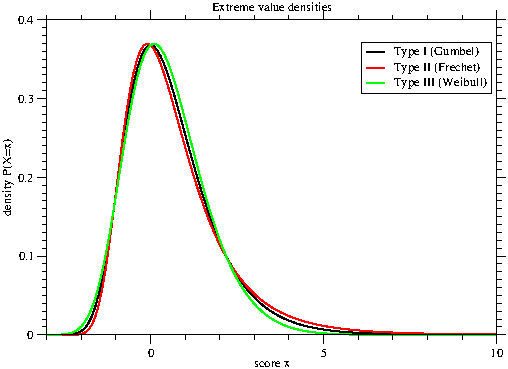
\includegraphics[width=2.8in]{figures/gev_density}
\end{minipage}
\begin{minipage}{3in}
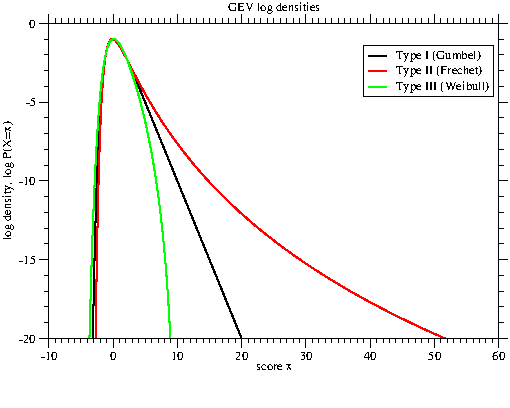
\includegraphics[width=2.8in]{figures/gev_logdensity}
\end{minipage}
}

For more details, see the excellent description in \citep{Coles01}.
Easel's $\{ \mu, \lambda, \alpha \}$ notation differs from the $\{
\mu, \sigma, \xi \}$ parameterization used by Coles. Use $\lambda =
\frac{1}{\sigma}$ and $\alpha = \xi$ to translate.

\subsection{Fitting GEV distributions to observed data}

Easel fits GEVs by maximum likelihood estimation by numerically
optimizing the log likelihood function, using first derivative
information and conjugate gradient descent.  See the \eslmod{gumbel}
chapter for a more general introduction to maximum likelihood fitting.

\subsubsection{Maximum likelihood estimation, complete data}

The function \ccode{esl\_gev\_FitComplete()} uses gradient information
to find parameters that optimize the likelihood function, using the
conjugate gradient descent code in the \eslmod{minimizer} module.

Given $n$ samples $x_1..x_n$, we want to estimate maximum likelihood
parameter estimates $\{ \hat{\mu}, \hat{\lambda}, \hat{\alpha} \}$
that maximize the log likelihood:

\begin{equation}
\log L(\lambda, \mu, \alpha) = n \log \lambda 
       - \frac{\alpha+1}{\alpha} 
           \sum_{i=1}^{n} \log\left[1+ \alpha\lambda(x_i - \mu) \right]
       - \sum_{i=1}^{n} \left[ 1 + \alpha\lambda (x_i - \mu) \right]^{\frac{1}{\alpha}}
\label{eqn:gev_logL}
\end{equation}

The $\left[ 1 + \alpha\lambda (x_i - \mu) \right]^{\frac{1}{\alpha}}$
term can be rewritten in a more conveniently differentiable form as
$\exp \left\{ \frac{1}{\alpha} \log \left[ 1 + \alpha\lambda (x_i - \mu)
\right] \right\}$.

Since the $\lambda$ parameter is constrained to $\lambda > 0$ but the
numerical optimizer expects unconstrained parameters, we use a change
of variables $\lambda = e^w$ and optimize an unconstrained value $w$.

The gradient of the log likelihood with respect to $\mu$, $w$, and
$\alpha$ is:

%% xref: STL9/118-120
\begin{eqnarray}
\frac{\partial \log L}{\partial \mu} & = &
  \sum_{i=1}^n \frac{\lambda (\alpha+1)}{1+\alpha\lambda(x_i-\mu)} 
 -\sum_{i=1}^n \lambda \exp 
    \left\{ -\frac{\alpha+1}{\alpha} \log
          \left[1+\alpha\lambda(x_i-\mu)\right] \right\}
\\%
\label{eqn:gev_mupartial}
\frac{\partial \log L}{\partial w} & = &
  n - \sum_{i=1}^{n} \frac{\lambda (\alpha+1) (x_i - \mu)} 
                          {1 + \alpha \lambda (x_i - \mu)}
  + \sum_{i=1}^n \lambda (x_i - \mu) 
         \exp \left\{ -\frac{\alpha+1}{\alpha} \log
          \left[1+\alpha\lambda(x_i-\mu)\right] \right\}
\\%
\label{eqn:gev_wpartial}
\frac{\partial \log L}{\partial \alpha} & = &
   \sum_{i=1}^n \left\{
      \begin{array}{l}
      - \frac{\alpha+1}{\alpha} \frac{\lambda(x_i-\mu)}
                                  {1 +\alpha\lambda(x_i-\mu)}\\
      + \frac{1}{\alpha^2} \log \left[ 1 + \alpha\lambda(x_i - \mu) \right]\\
      + \frac{1}{\alpha} \frac{\lambda(x_i-\mu)}
                          {1 +\alpha\lambda(x_i-\mu)}
      e^{-\frac{1}{\alpha} \log\left[ 1 + \alpha\lambda(x_i - \mu) \right]}\\
     -  \frac{1}{\alpha^2} \log \left[ 1 + \alpha\lambda(x_i - \mu) \right]
      e^{-\frac{1}{\alpha} \log\left[ 1 + \alpha\lambda(x_i - \mu)
	 \right]} 
     \end{array}
     \right.
\\%
\label{eqn:gev_alphapartial}
\end{eqnarray}

When $|\alpha\lambda(x_i - \mu)|$ approaches $0$, the GEV approximates
a Gumbel distribution and these equations can be simplified using the
approximation $\log(1+a) \simeq a$.








\subsection{Functions in the gev module}
\input{autotext/esl_gev_functions}

\newpage
\section{\eslmod{gumbel}: Type I extreme value (Gumbel) statistics}

The scores of local sequence alignments often follow a Gumbel
distribution, so Gumbel statistics are often used to estimate the
statistical significance of alignment scores.

The Gumbel distribution is the so-called Type I extreme value
distribution (EVD). It occurs so frequently in sequence analysis
applications, compared to the type II (Fr\'{e}chet) and type III
(Weibull) extreme value distributions, that ``Gumbel'' and ``EVD'' are
often used interchangeably in bioinformatics. Easel has a separate
module, the \eslmod{gev} module, that implements the generalized
extreme value distribution.

\emph{Karlin/Altschul} statistics are a special case of the Gumbel
distribution that apply to the scores of ungapped local alignments
between infinitely long random sequences. Karlin/Altschul statistics
also apply reasonably well to the more useful case of gapped alignment
of finite-length sequences. Karlin/Altschul statistics predict how the
Gumbel's two parameters depend on the length of the query and target
sequences. In the case of ungapped alignments, Karlin/Altschul
statistics allow the Gumbel parameters to be estimated directly,
without the need for a compute-intensive simulation.

\subsection{The gumbel API}

The \eslmod{gumbel} API consists of the following functions:

\vspace{0.5em}
\begin{center}
\begin{tabular}{ll}\hline
    \multicolumn{2}{c}{\textbf{evaluating densities and distributions:}}\\
\ccode{esl\_gumbel\_pdf()}     & Returns the probability density, $P(S=x)$.\\
\ccode{esl\_gumbel\_logpdf()}  & Returns the log of the pdf, $\log P(S=x)$.\\
\ccode{esl\_gumbel\_cdf()}     & Returns the cumulative probability distribution, $P(S \leq x)$.\\
\ccode{esl\_gumbel\_logcdf()}  & Returns the log of the cdf, $\log P(S \leq x)$.\\
\ccode{esl\_gumbel\_surv()}    & Returns right tail mass, 1-cdf, $P(S > x)$\\
\ccode{esl\_gumbel\_logsurv()} & Returns log of 1-cdf, $\log P(S > x)$.\\
    \multicolumn{2}{c}{\textbf{sampling:}}\\
\ccode{esl\_gumbel\_Sample()}  & Returns a Gumbel-distributed random sample.\\
    \multicolumn{2}{c}{\textbf{maximum a posteriori parameter fitting:}}\\
\ccode{esl\_gumbel\_FitComplete()} & Estimates $\mu,\lambda$ from complete data.\\
\ccode{esl\_gumbel\_FitCensored()} & Estimates $\mu,\lambda$ from censored data.\\
\ccode{esl\_gumbel\_FitTruncated()}& Estimates $\mu,\lambda$ from truncated data.\\\hline
\end{tabular}
\end{center}
\vspace{0.5em}

The Gumbel distribution depends on two parameters, $\mu$ and
$\lambda$. When $\mu$ and $\lambda$ are known, the statistical
significance (P-value) of a single score $x$ is $P(S>x)$, obtained by
a call to \ccode{esl\_gumbel\_surv()}.  The E-value for obtaining that
score or better in searching a database of $N$ sequences is just
$NP(S>x)$.

When $\mu$ and $\lambda$ are unknown, they are estimated from scores
obtained from comparisons of simulated random data. (Analytical
solutions for $\mu$ and $\lambda$ are only available in the case of
ungapped sequence alignments.)  The \ccode{esl\_evd\_Fit*()} functions
provide maximum likelihood parameter fitting routines for different
types of data. 

\subsubsection{Augmentations: random, minimizer}

The \ccode{esl\_gumbel\_Sample()} function requires augmenting with the
\eslmod{random} module.

The \ccode{esl\_gumbel\_FitTruncated()} function requires augmenting
with the \eslmod{minimizer} module.


\subsection{Example of using the gumbel API}

An example that samples 10,000 data points from a Gumbel distribution
with $\mu=-20$, $\lambda=0.4$; reports the min and max samples, and
the probability mass to the left of the min and to the right of the
max (both of which should be about $\frac{1}{10000}$, since we took
10,000 samples); and then fits those simulated data to a Gumbel and
reports the fitted $\mu$ and $\lambda$:

\input{cexcerpts/gumbel_example}



\subsection{Extreme value densities}

The probability density function (pdf) and the cumulative distribution
function (cdf) of the extreme value distribution are:

\begin{equation}
P(x) = \lambda \exp \left[ -\lambda (x - \mu) - e^{- \lambda (x - \mu)} \right]
\label{eqn:density}
\end{equation}

\begin{equation}
P(S < x) = \exp \left[ -e^{-\lambda(x - \mu)} \right]
\label{eqn:distribution}
\end{equation}

The extreme value density and distribution functions for $\mu = 0$ and
$\lambda = 1.0$ are shown below.

\begin{center}
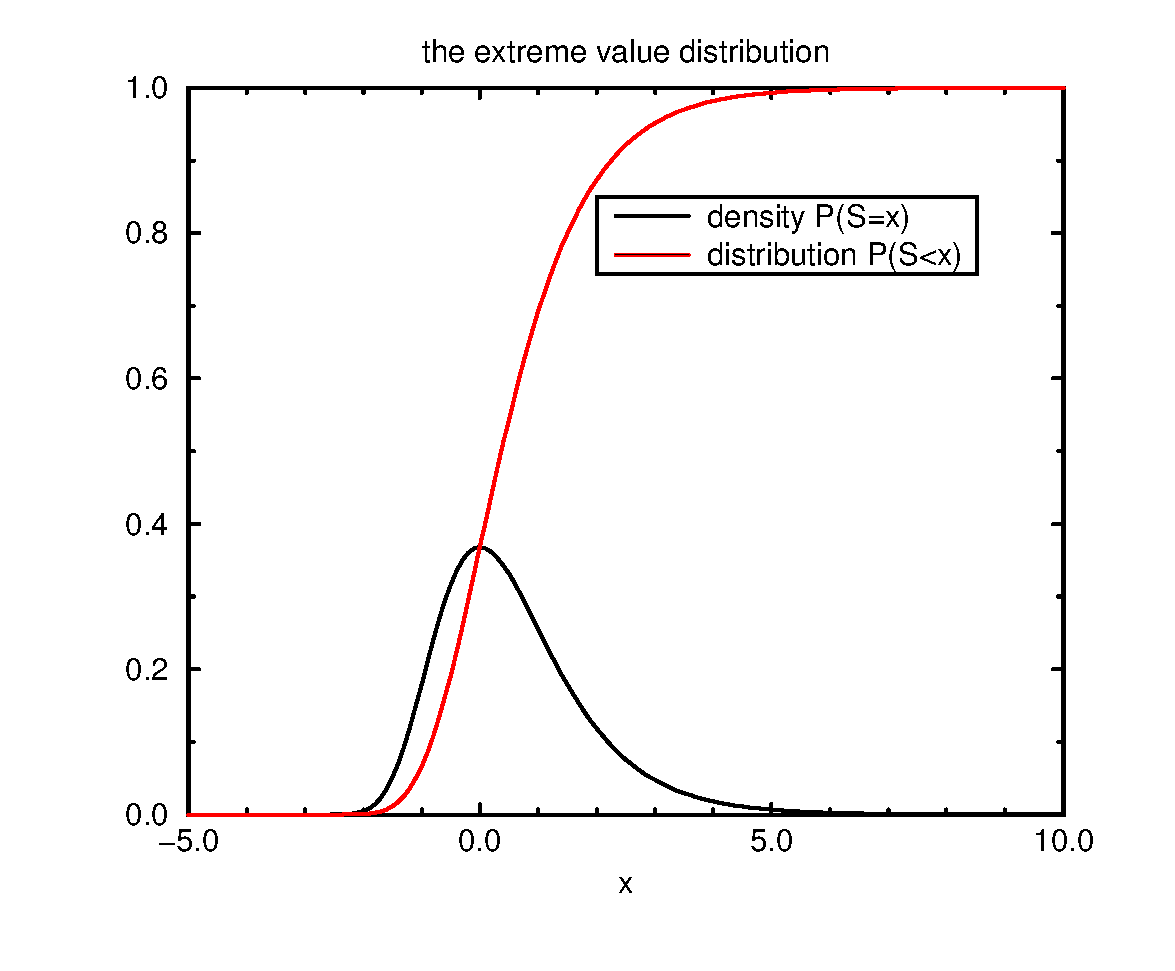
\includegraphics[width=3in]{figures/evd_basic}
\end{center}

The $\mu$ and $\lambda$ parameters are {\em location} and {\em scale}
parameters, respectively:

\centerline{
\begin{minipage}{3in}
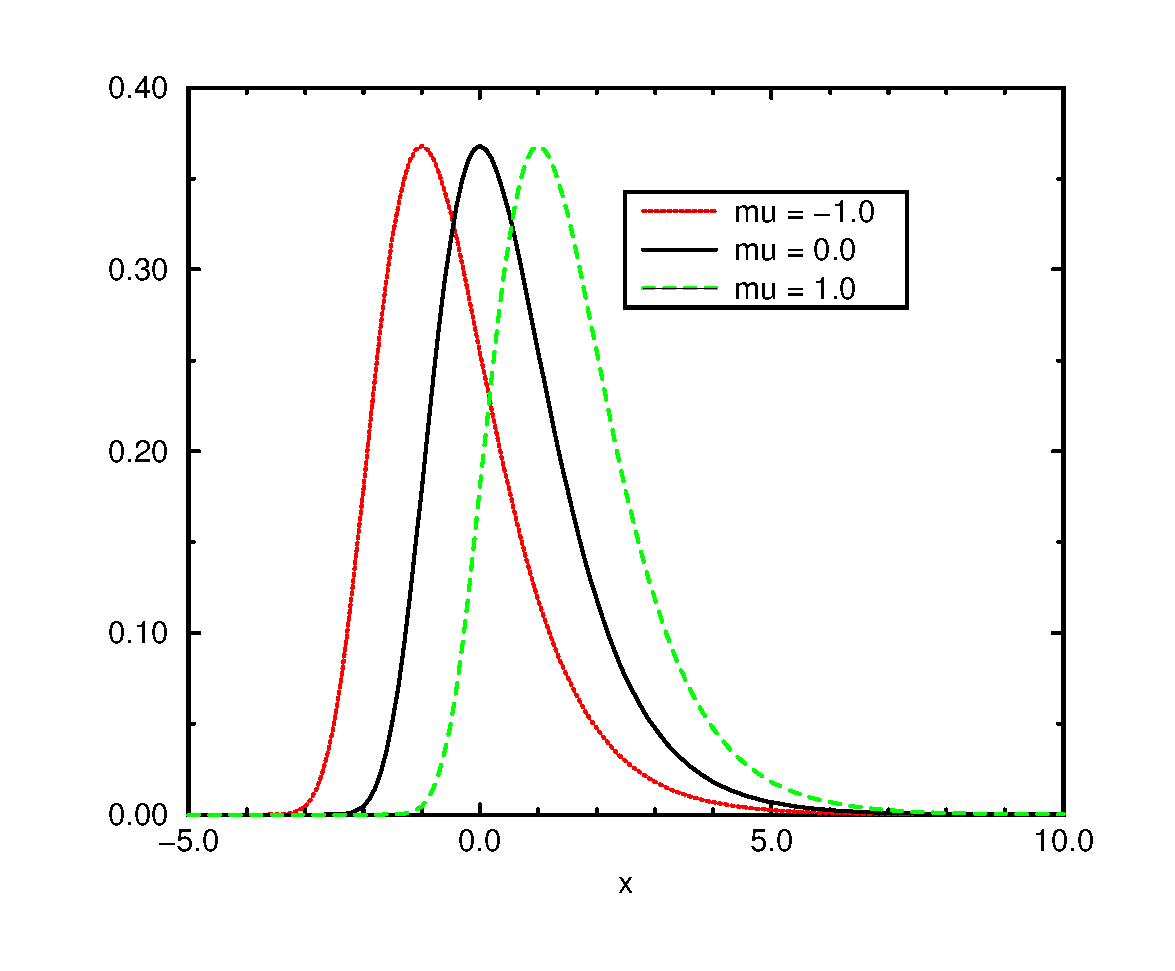
\includegraphics[width=2.8in]{figures/evd_location}
\end{minipage}
\begin{minipage}{3in}
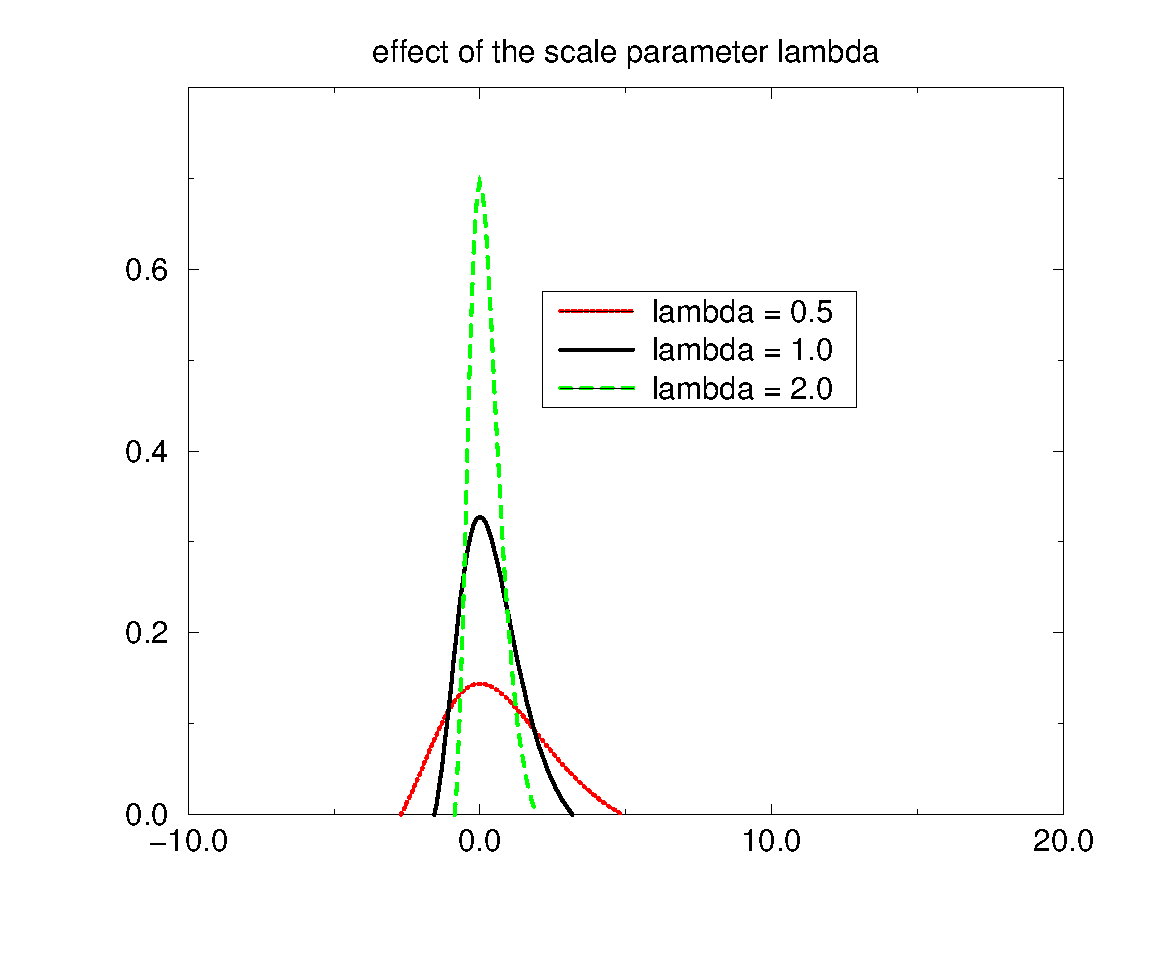
\includegraphics[width=2.8in]{figures/evd_scale}
\end{minipage}
}

Gumbel distributions can have their long tail to the right or to the
left. The form given here is for the long tail to the right.  This is
the form that arises when the extreme value is a maximum, such as when
our score is the maximum over the individual scores of all possible
alignments. The equations in \citep{Lawless82} are for extremal
minima; use $(x - u) = -(x - \mu)$ and $b = 1 / \lambda$ to convert
Lawless' notation to the notation used here.





\subsection{Fitting Gumbel distributions to observed data}

Given a set of $n$ observed samples $\mathbf{x}$, we may want to
estimate the $\mu$ and $\lambda$ parameters.

One might try to use linear regression to fit to a $\log \log$
transformation of the $P(S < x)$ histogram, which gives a straight
line with slope $-\lambda$ and $x$ intercept $\mu$:

\begin{equation}
\log \left[ -\log P(S<x) \right] = -\lambda x + \lambda \mu
\end{equation}

However, the linear regression method is undesirable because it is
sensitive to outliers. The following table shows the \% error for
estimating $\hat{\mu}$ and $\hat{\lambda}$ from 500 simulated complete
datasets, sampled from a Gumbel with $\mu = -20.0$ and $\lambda =
0.4$, for four different dataset sizes:

\begin{center}
\begin{tabular}{lrrrr} \hline
                              & \multicolumn{4}{c}{\# of samples}\\
                              & 100 & 1000  & 10,000 & 100,000 \\
\% error in $\hat{\mu}$       &  2\%&   1\% & 0.9\%  &  0.9\%  \\
max error in $\hat{\mu}$      & 24\%&  13\% &  10\%  &   10\%  \\
\% error in $\hat{\lambda}$   & 12\%&   7\% &   5\%  &    3\%  \\
max error in $\hat{\lambda}$  & 49\%&  33\% &  25\%  &   20\%  \\ \hline
\end{tabular}
\end{center}


A better rough estimate of $\hat{\mu}$ and $\hat{\lambda}$ can be
obtained from the sample mean $m$ and variance $s^2$ of the observed
data \citep{Evans00}:\footnote{All simulation data are generated by
the \eslmod{evd} module's stats driver. The only exception is the
linear regression fit data, which come from an old version of HMMER.}

\begin{eqnarray*}
  \hat{\lambda} & = & \frac{\pi}{\sqrt{6s^2}}\\
  \hat{\mu}     & = & m - \frac{0.57722}{\hat{\lambda}}
\end{eqnarray*}

The mean/variance method is more accurate than linear regression, as
shown by the following simulation results:

\begin{center}
\begin{tabular}{lrrrr} \hline
                              & \multicolumn{4}{c}{\# of samples}\\
                              & 100 & 1000  & 10,000 & 100,000 \\
\% error in $\hat{\mu}$       &  1\%& 0.3\% &  0.1\% & 0.03\%  \\
max error in $\hat{\mu}$      &  5\%&   1\% &  0.4\% &  0.1\%  \\
\% error in $\hat{\lambda}$   &  9\%&   3\% &  0.8\% &  0.3\%  \\
max error in $\hat{\lambda}$  & 40\%&  12\% &    3\% &  0.9\%  \\ \hline
\end{tabular}
\end{center}

Still, the mean/variance method is not as accurate as a maximum
likelihood estimation (especially for $\lambda$). Also, it requires
complete data, whereas we also need to solve problems where we fit to
\emph{truncated} or \emph{censored} data. Easel's main estimation
methods are therefore maximum likelihood methods.

\subsubsection{Maximum likelihood estimation, complete data}

Given $n$ samples $x_1..x_n$ from some distribution that depends on
parameters $\theta$, we want to estimate maximum likelihood parameter
estimates $\hat{\theta}$ that maximize the log likelihood:

\[
   \hat{\theta} = \argmax_{\theta} \sum_{i=1}^{n} \log P(x_i \mid \theta)
\]

These are also \emph{maximum a posteriori} parameter estimates, if we
assume a uniform prior $P(\theta)$.

Specifically, for samples $x_i$ drawn from an extreme value
distribution, the log likelihood to optimize is:

\begin{equation}
\log L(\lambda, \mu) = n \log \lambda - \sum_{i=1}^{n} \lambda(x_i -
\mu) - \sum_{i=1}^{n} e^{-\lambda(x_i - \mu)}
\label{eqn:logL}
\end{equation}

This objective function is differentiable with respect to $\mu$ and
$\lambda$:

\begin{eqnarray}
\frac{\partial \log L}{\partial \mu} & = &
n \lambda - \lambda \sum_{i=1}^{n} e^{-\lambda (x_i - \mu)}\\%
\\%
\label{eqn:mupartial}
\frac{\partial \log L}{\partial \lambda} & = &
\frac{n}{\lambda} - \sum_{i=1}^{n} (x_i - \mu) +  
\sum_{i=1}^{n} (x_i - \mu) e^{-\lambda (x_i - \mu)}
\label{eqn:lambdapartial}
\end{eqnarray}

The maximum likelihood estimates $\hat{\lambda}$ and $\hat{\mu}$ are
the solutions to $\frac{\partial \log L}{\partial \mu} = 0$ and
$\frac{\partial \log L}{\partial \lambda} = 0$. Lawless
\citep{Lawless82} gives a useful trick here that lets us solve both of
these simultaneously. When (\ref{eqn:mupartial}) is set to zero, it
can be used to get $\hat{\mu}$ in terms of $\hat{\lambda}$:

\begin{eqnarray}
e^{-\hat{\lambda} \hat{\mu}} & = & \frac{1}{n} \sum_{i=1}^{n} e^{-\hat{\lambda} x_i} 
\label{eqn:substitute}\\
\hat{\mu} & = & - \frac{1}{\hat{\lambda}} 
	\log \left[ \frac{1}{n} \sum_{i=1}^{n} e^{-\hat{\lambda} x_i} \right]
\label{eqn:solvemu}
\end{eqnarray}

Substituting (\ref{eqn:substitute}) into (\ref{eqn:lambdapartial}),
gives us an equation for solving $\hat{\lambda}$ in terms of the
$x_i$'s:

\begin{eqnarray}
\frac{1}{\hat{\lambda}} - \frac{1}{n} \sum_{i=1}^{n} x_i +
\frac{\sum_{i=1}^{n} x_i e^{-\hat{\lambda} x_i}}
     {\sum_{i=1}^{n} e^{-\hat{\lambda} x_i}} 
& = & 0
\label{eqn:newtontarget}
\end{eqnarray}

This is our target function. We could solve it readily enough (by
bisection search, for example) and obtain $\hat{\lambda}$. We can
solve it even faster using the Newton/Raphson algorithm, because it is
differentiable with respect to lambda:

\begin{equation}
\frac{d}{d\hat{\lambda}} = 
\frac{\left( \sum_{i=1}^{n} x_i e^{-\hat{\lambda} x_i} \right)^2 } 
     {\left( \sum_{i=1}^{n} e^{-\hat{\lambda} x_i}     \right)^2 }
-
\frac{\sum_{i=1}^{n} x_i^2 e^{-\hat{\lambda} x_i}}
     {\sum_{i=1}^{n} e^{-\hat{\lambda} x_i}}
-
\frac{1}{\hat{\lambda}^2}
\label{eqn:newtonderivative}
\end{equation}

Now, the key equations are (\ref{eqn:solvemu}),
(\ref{eqn:newtontarget}), and (\ref{eqn:newtonderivative}). In
summary, the inference procedure is the following:

\begin{itemize}
\item Guess an initial $\hat{\lambda}$ (using the mean/variance
  method, for example, but any reasonable guess works).
\item Use Newton/Raphson iterations to find the $\hat{\lambda}$ that satisfies
      (\ref{eqn:newtontarget}):
	\begin{itemize}
	\item calculate the target function $f$ and 
         its first derivative $f'$ at $\hat{\lambda}$, using 
	(\ref{eqn:newtontarget}) to calculate $f$ and 
	(\ref{eqn:newtonderivative}) to calculate $f'$.
	\item If $f$ is within some absolute tolerance of zero 
	(e.g., $10^{-6}$), stop; we have found $\hat{\lambda}$.
	\item Else, estimate a new $\hat{\lambda} = \hat{\lambda} - \frac{f}{f'}$,
	  and do another iteration.
	\end{itemize}
\item Plug $\hat{\lambda}$ into (\ref{eqn:solvemu}) to get $\hat{\mu}$.
\end{itemize}

This algorithm is implemented in \ccode{esl\_evd\_FitComplete()}.  An
auxiliary function, \ccode{lawless416()}, calculates the target
function and its derivative (equations (\ref{eqn:newtontarget}) and
(\ref{eqn:newtonderivative})) given the current estimate of
$\hat{\lambda}$.  The name comes from Lawless' equation 4.1.6, the
target function \citep{Lawless82}.

The accuracy of fitting to simulated data (generated with $\mu=-20$
and $\lambda=0.4$), collated over 500 simulations, is shown in the
following table:

\begin{center}
\begin{tabular}{lrrrr} \hline
                              & \multicolumn{4}{c}{\# of samples}\\
                              & 100 & 1000  & 10,000 & 100,000 \\
\% error in $\hat{\mu}$       &  1\%& 0.3\% &  0.1\% & 0.03\%  \\
max error in $\hat{\mu}$      &  4\%&   2\% &  0.5\% &  0.1\%  \\
\% error in $\hat{\lambda}$   &  6\%&   2\% &  0.6\% &  0.2\%  \\
max error in $\hat{\lambda}$  & 36\%&   9\% &    2\% &  0.8\%  \\ \hline
\end{tabular}
\end{center}





\subsubsection{Maximum likelihood fitting to censored data}

A \emph{censored} data problem is when we have $N$ samples, but we
only observe the values of a subset of $n$ samples $x_1..x_n$ that are
greater or equal to some cutoff $\phi$. The remaining $z = N-n$
samples are \emph{censored}, and for these we only know that $x <
\phi$.  $x_i..x_n$, $n$, $\phi$, and $z$ are all known in a censored
data problem.

To estimate maximum likelihood parameters $\hat{\theta}$ for some
distribution from censored data \citep{Gelman95}, the log likelihood
to maximize is:


\[ 
  \hat{\theta} = \argmax_{\theta} z \log P(x<\phi \mid \theta)
                         + \sum_{i=1}^n \log P(x_i \mid \theta)
\]

Specifically, when fitting a Gumbel distribution, the log likelihood
to optimize is:

\begin{equation}
  \log L(\lambda, \mu) = 
    n \log \lambda 
     - z e^{-\lambda(\phi - \mu)}
     - \sum_{i=1}^{n} \lambda(x_i - \mu) 
     - \sum_{i=1}^{n} e^{-\lambda(x_i - \mu)}
\label{eqn:censor_logL}
\end{equation}

To optimize this, we follow a similar procedure as used for complete
data \citep{Lawless82}. The log likelihood is differentiable with
respect to $\lambda$ and $\mu$:

\begin{eqnarray}
\frac{\partial \log L}{\partial \mu} & = &
n \lambda  
- z \lambda e^{-\lambda (\phi - \mu)}
- \lambda \sum_{i=1}^{n} e^{-\lambda (x_i - \mu)}
\label{eqn:censor_dmu}
\\%
\frac{\partial \log L}{\partial \lambda} & = &
\frac{n}{\lambda} 
+ z (\phi - \mu) e^{-\lambda (\phi - \mu)}
- \sum_{i=1}^{n} (x_i - \mu) 
+ \sum_{i=1}^{n} (x_i - \mu) e^{-\lambda (x_i - \mu)}
\label{eqn:censor_dlambda}
\end{eqnarray}

Setting (\ref{eqn:censor_dmu}) to zero and solving for $\hat{\mu}$ in
terms of $\hat{\lambda}$ gives:

\begin{equation}
\hat{\mu}  =  - \frac{1}{\hat{\lambda}} 
	\log \left[ \frac{1}{n} 
	\left( z e^{-\hat{\lambda} \phi} 
               + \sum_{i=1}^{n} e^{-\hat{\lambda} x_i} \right)
	\right]
\label{eqn:censor_solvemu}
\end{equation}

Substituting (\ref{eqn:censor_solvemu}) into
(\ref{eqn:censor_dlambda}) gives the target equation:

\begin{equation}
\frac{1}{\hat{\lambda}} 
- \frac{1}{n} \sum_{i=1}^{n} x_i +
\frac{z \phi e^{-\hat{\lambda} \phi} + \sum_{i=1}^{n} x_i e^{-\hat{\lambda} x_i}} 
     {z e^{-\hat{\lambda} \phi} + \sum_{i=1}^{n} e^{-\hat{\lambda} x_i}} 
 =  0
\label{eqn:censor_newtontarget}
\end{equation}

To use Newton-Raphson root finding (instead of a slower bisection
search) we also need the first derivative of this target equation with
respect to $\lambda$:

\begin{equation}
\frac{d}{d\hat{\lambda}} = 
\frac{\left( 
        z \phi e^{-\hat{\lambda} \phi}
        + \sum_{i=1}^{n} x_i e^{-\hat{\lambda} x_i} 
       \right)^2 } 
     {\left( 
        z e^{-\hat{\lambda} \phi}
        + \sum_{i=1}^{n} e^{-\hat{\lambda} x_i}     
       \right)^2 }
-
\frac{z \phi^2 e^{-\hat{\lambda} \phi} + \sum_{i=1}^{n} x_i^2 e^{-\hat{\lambda} x_i}}
     {z  e^{-\hat{\lambda} \phi} + \sum_{i=1}^{n} e^{-\hat{\lambda} x_i}}
-
\frac{1}{\hat{\lambda}^2}
\label{eqn:censor_newtonderiv}
\end{equation}

In summary: given $n$ observed samples $x_1..x_n$ from a total sample
of $N$ samples, $z = N-n$ of which were censored because they have
values $< \phi$, we solve for maximum likelihood estimates
$\hat{\lambda}$ and $\hat{\mu}$ using the same procedure we used for
complete data, by using equations (\ref{eqn:censor_solvemu}),
(\ref{eqn:censor_newtontarget}), and (\ref{eqn:censor_newtonderiv}) in
place of equations (\ref{eqn:solvemu}), (\ref{eqn:newtontarget}), and
(\ref{eqn:newtonderivative}). Easel implements this procedure in
\ccode{esl\_evd\_FitCensored()}.  The target function
(\ref{eqn:censor_newtontarget}) and its derivative
(\ref{eqn:censor_newtonderiv}) are implemented in the auxiliary
function \ccode{lawless422()} \citep{Lawless82}.

Results on 500 simulated datasets with $\mu = -20, \lambda = 0.4$,
censored at $\phi = -20$ -- the expected peak of the histogram; that
is, a censored fit only to the right tail, which contains about 63\%
of the samples:

\begin{center}
\begin{tabular}{lrrrr} \hline
 & \multicolumn{4}{c}{\# samples in EVD histogram}\\
                        & 100 & 1000  & 10,000 & 100,000 \\
\% error in $\mu$       &  1\%& 0.4\% &  0.1\% &  0.04\%  \\
max error in $\mu$      &  5\%&   2\% &  0.5\% &  0.2\%  \\
\% error in $\lambda$   &  9\%&   3\% &  0.9\% &  0.3\%  \\
max error in $\lambda$  & 33\%&  11\% &    3\% &    1\%  \\ \hline
\end{tabular}
\end{center}

\subsubsection{Maximum likelihood fitting to truncated data}

A \emph{truncated} dataset is when we only observe $n$ samples $x_i$,
and an \emph{unknown} number $z$ of samples less than some threshold
$\phi$ were unobserved. Thus, only the right tail of $n$ samples $x_i
\geq \phi$ as observed. In a truncated dataset, $x_1..x_n$, $n$, and
$\phi$ are known, but $z$ is unknown.

Solving a truncated data problem motivates a Bayesian approach,
because we need to integrate out (marginalize) the nuisance $z$
parameter, and to do this, we have to specify a prior distribution for
$P(z)$. Gelman \emph{et al.} describe a general Bayesian framework for
thinking about various types of missing data problems, including
censored and truncated data \citep{Gelman95}.

In short, to obtain maximum likelihood parameters $\hat{\theta}$ for
some distribution, given truncated data, the log likelihood we wish to
maximize is:

\begin{equation}
  \hat{\theta} = \argmax_\theta -n \log P(x \geq \phi \mid \theta) 
                   + \sum_{i=1}^n \log P(x_i \mid \theta).
\label{eqn:truncated_objective}
\end{equation}

\textbf{Detour: derivation of the truncated data likelihood}

The derivation of the above equation may not be immediately obvious.
The presence of the $n P(x \geq \phi \mid \theta)$ term may be
counterintuitive, as opposed to the more intuitive $z P(x < \phi \mid
\theta)$ term that accounts for the missing data in a censored data
problem. Gelman \emph{et al.} actually don't even show the equation in
their book; I obtained it from an exercise solution on their web site.
To convince you (and to remind me) of its correctness, a sketch of the
derivation follows.

We start with the same likelihood equation that arises in censored
data for a \emph{known} total number of samples $N$ (where $N=n+z$),
but since $N$ is unknown, we need to integrate over all possible $N$
from $n$ to $\infty$:

\begin{eqnarray*}
   P(\mathbf{x} \mid \theta, \phi) & = &
    \sum_{N=n}^{\infty}   P(\mathbf{x} \mid \theta, \phi, N) P(N)\\
   & = & 
    \prod_{i=1}^n P(x_i \mid \theta) 
    \left[
      \sum_{N=n}^\infty {N \choose n} P(x < \phi \mid \theta)^{N-n} P(N)
    \right]\\
\end{eqnarray*}

The $\prod_{i=1}^n P(x_i \mid \theta)$ is straightforward; that sum is
our problem. The trick is to rearrange it so we can treat it as a
convergent negative binomial series:

\[
   (1-p)^{-a} = 1 + ap + \frac{a(a+1)}{2!} p^2 +
   \frac{a(a+1)(a+2)}{3!} p^3...
\]

To get the sum into the form of this series, Gelman \emph{et al.}
suggest using an informative prior $P(N) = \frac{1}{N}$, an apparently
unmotivated choice that happens to make the sum collapse nicely:

\begin{eqnarray*}
 &=& P(N=n) 
    + (n+1) P(x < \phi \mid \theta) P(N=n+1) 
    + \frac{(n+1)(n+2)}{2!} P(x < \phi \mid \theta)^2 P(N=n+2) ...\\
 &= & \frac{1}{n} \left[
      1 
      + n P(x < \phi \mid \theta)
      + \frac{n(n+1)}{2!} P(x < \phi \mid \theta)^2 
      + \frac{n(n+1)(n+2)}{3!} P(x < \phi \mid \theta)^3 \right]\\
 &=& \frac{1}{n} (1 - P(x < \phi \mid \theta))^{-n}\\
 &=& \frac{1}{n} P(x \geq \phi \mid \theta)^{-n}\\
\end{eqnarray*}

The $\frac{1}{n}$ is a constant, so we drop it from the likelihood
equation we'll maximize. Putting this term back together with the
probability of the observed data and taking the log, we obtain the log
likelihood in equation (\ref{eqn:truncated_objective}).

Alternatively, we might choose an uninformative improper uniform prior
$P(N) \propto 1$. This gives a log likelihood that only differs by a
term of $n+1$ versus $n$:

\begin{equation}
  \hat{\theta} = \argmax_\theta -(n+1) \log P(x \geq \phi \mid \theta) 
                   + \sum_{i=1}^n \log P(x_i \mid \theta).
\end{equation}

However, empirically, this form is ineffective, at least for fitting
Gumbels. The $\frac{1}{N}$ prior performs much better, probably
because it constrains the solutions to favor smaller, finite, more
reasonable choices of $N$.



\textbf{Back to fitting a truncated Gumbel}

For the specific case of fitting a truncated Gumbel, the log
likelihood (\ref{eqn:truncated_objective}) to optimize is:

\[
  \log L(\lambda, \mu) =
     n \log \lambda 
     - \sum_{i=1}^{n} \lambda(x_i - \mu) 
     - \sum_{i=1}^{n} e^{-\lambda(x_i - \mu)}
     - n \log (1 - \exp(-e^{-\lambda(\phi - \mu)}))
\label{eqn:truncated_logL}
\]

This is differentiable with respect to $\lambda$ and $\mu$, but it's
not going to reduce to the clean root-finding problem that we obtained
for complete data or censored data. Instead we're going to be left
with a numerical optimization problem. We can use standard numerical
optimization code, such as steepest descent or conjugate gradient
descent. There's just one hitch. These algorithms assume unconstrained
parameters, but $\lambda$ is constrained to values $>0$. We do a
change of variables, and use the transformation $\lambda = e^w$ so we
can optimize the unconstrained parameter $w = \log \lambda$ instead of
optimizing $\lambda$ directly.  The necessary partial derivatives are
then:

\begin{eqnarray}
\frac{\partial \log L}{\partial \mu} & = &
n \lambda  
- \lambda \sum_{i=1}^{n} e^{-\lambda (x_i - \mu)}
- \frac{n \lambda \exp \left[ -\lambda (\phi - \mu) - e^{- \lambda (\phi - \mu)} \right]}
       {1 - \exp(-e^{-\lambda(\phi - \mu)})}
\label{eqn:truncated_dmu}
\\%
\frac{\partial \log L}{\partial w} & = &
n 
- \sum_{i=1}^{n} \lambda(x_i - \mu) 
+ \sum_{i=1}^{n} \lambda(x_i - \mu) e^{-\lambda (x_i - \mu)}
+ \frac{n\lambda (\phi-\mu) \exp \left[ -\lambda (\phi - \mu) - e^{- \lambda (\phi - \mu)} \right]}
       {1 - \exp(-e^{-\lambda(\phi - \mu)})}
\label{eqn:truncated_dw}
\end{eqnarray}

This optimization is carried out by \ccode{esl\_evd\_FitTruncated()}.
The likelihood (\ref{eqn:truncated_logL}) is implemented in
\ccode{tevd\_func()}, and the derivatives (\ref{eqn:truncated_dmu}) and
(\ref{eqn:truncated_dw}) are implemented in \ccode{tevd\_dfunc()}.
\ccode{esl\_evd\_FitTruncated()} simply sets up the problem and passes
it all off to a conjugate gradient descent optimizer.

Results on 500 simulated datasets with $\mu = -20, \lambda = 0.4$,
truncated at $\phi = -20$ (leaving the right tail, containing about
63\% of the samples):

\begin{center}
\begin{tabular}{lrrrr} \hline
                              & \multicolumn{4}{c}{\# samples}\\
                              & 100 & 1000  & 10,000 & 100,000 \\
\% error in $\hat{\mu}$       & 13\%&   2\% &  0.8\% &  0.3\%  \\
max error in $\hat{\mu}$      &260\%&  42\% &    3\% &    1\%  \\
\% error in $\hat{\lambda}$   & 15\%&   5\% &    2\% &  0.6\%  \\
max error in $\hat{\lambda}$  & 68\%&  18\% &    6\% &    2\%  \\ \hline
\end{tabular}
\end{center}

Fitting truncated Gumbel distributions is difficult, requiring much
more data than fitting complete or censored data. The problem is that
the right tail becomes a scale-free exponential when $\phi >> \mu$,
and $\mu$ becomes undetermined. Fits become very inaccurate as $\phi$
gets larger than $\mu$, and for sufficiently large $\phi$, the
numerical optimizer will completely fail.








\subsection{Functions in the gumbel module}
\input{autotext/esl_gumbel_functions}

\newpage
\section{\eslmod{hyperexp}: Hyperexponential distributions}

The hyperexponential (mixture exponential) distribution may be useful
for fitting fat-tailed empirical distributions. 

\subsection{Hyperexponential densities}

The hyperexponential distribution is a mixture of $K$ independent
exponentials with a common location $\mu$ and different decay
constants $\lambda_k$.

The probability density function (PDF) is:

\begin{equation}
P(X=x) = \sum_k^{K} q_k \lambda_k e^{- \lambda_k (x - \mu)}
\label{eqn:hyperexp_pdf}
\end{equation}

The cumulative distribution function (CDF) is:

\begin{equation}
P(X \leq x) = \sum_k^{K} q_k (1 - e^{- \lambda_k (x - \mu)})
\label{eqn:hyperexp_cdf}
\end{equation}

Variate $x$ ranges $\mu \leq x < \infty$.

Mixture coefficients $q_k$ specify the prior probability of each
component $k$; $0 \leq q_k \leq 1$ and $\sum_k q_k = 1$.

The single location parameter $\mu$ is unconstrained, $-\infty < \mu <
\infty$. (Exponential distributions are usually represented without an
explicit location parameter, implicitly assuming $\mu = 0$.)

The scale parameters $\lambda_k$ for each component are nonnegative,
$\lambda_k > 0$.



\subsection{Functions in the hyperexp module}
\input{autotext/esl_hyperexp_functions}

\newpage
\section{\eslmod{mixdchlet}: Mixture Dirichlet distributions}
%\documentclass[11pt]{article}
\setcounter{secnumdepth}{0}

\usepackage{relsize}

\newcommand{\mono}[1]{{\smaller\texttt{#1}}}                    % literal (to be typed): code, program names

\begin{document}

\section{Fitting a mixture Dirichlet to counts}

\mono{esl\_mixdchlet\_Fit()} infers a maximum likelihood mixture
Dirichlet distribution for a data set of count vectors. It uses
conjugate gradient descent from an initial starting point. The result
is only a local optimum, so we typically run it multiple times with
different starting points. The partial derivatives of the log
likelihood function are persnickety, and the purpose of these notes is
to enshrine the derivation that corresponds to the implementation.

We have $N$ count vectors $c_i$, with each vector consisting of $K$
counts for individual symbols $c_{ia} \geq 0$. The mixture Dirichlet
$\theta$ consists of $Q$ components $\alpha_k$, with each parameter
vector containing $K$ parameters $\alpha_{ka} > 0$, and $Q$ mixture
coefficients $q_k > 0, \sum_k q_k = 1$.

The log likelihood of the data is:

\[
  L = \log P(\mbox{data} \mid \theta) = \sum_i \log P(c_i \mid \theta) = \sum_i \log \sum_k q_k P(c_i \mid \alpha_k)
\]

\mono{esl\_mixdchlet\_logpdf\_c()} calculates $\log P(c_i \mid
\theta)$.

$P(c_i \mid \alpha_k)$, the probability of one count vector given one
Dirichlet component, is:

\[
P(c_i \mid \alpha_k) = \frac{ |c_i|! }
                            { \prod_a c_{ia}! }
                       \frac{ \prod_a \Gamma \left( c_{ia} + \alpha_{ia} \right) }
                            { \Gamma ( |c_i + \alpha_k| ) }
                       \frac{ \Gamma ( |\alpha_k| ) }
                            { \prod_a \Gamma \left( \alpha_{ka} \right) }
\]

\mono{esl\_dirichlet\_logpdf\_c()} calculates $\log P(c_i \mid \alpha_k)$.

The conjugate gradient descent code works with unconstrained
real-valued parameters. The Dirichlet parameters $\alpha_{ka}$ are
constrained to $>0$, and mixture coefficients $q_k$ are constrained to
$>0$ and $\sum_k q_k = 1$. Define a change of variables in terms of
unconstrained parameters $\lambda_k$ for the mixture coefficients and
$\beta_{ka}$ for Dirichlet parameters:

\begin{eqnarray*}
  q_k          & = & \frac{ e^{\lambda_k} } { \sum_m e^{\lambda_m} } \\
  \alpha_{ka}  & = & e^{\beta_{ka}} 
\end{eqnarray*}

After variable substitution, partial differentiation w.r.t. the
unconstrained parameters, and substituting back the original
parameters, we have for the mixture coefficients:

\[
  \frac{\partial L}{\partial \lambda_k} = \sum_i P(k \mid \theta, c_i) - q_k
\]

i.e., the difference between the posterior probability of component
$k$ $P(k \mid \theta, c_i)$, calculated by \mono{mixdchlet\_postq()},
and its prior $q_k$.

For the Dirichlet parameters:

\[
\frac{\partial L}{\partial \beta_{ka}}  =  \sum_i
 \alpha_{ka} P(k \mid \theta, c_i) 
    \left( \Psi \left( c_{ia} + \alpha_{ka} \right)  
        -  \Psi \left( | c_i | + | \alpha_k | \right)
        +  \Psi \left( | \alpha_k | \right) 
        -  \Psi \left( \alpha_{ka} \right) 
    \right) 
\]


$\Psi(x)$ is the digamma function $\frac{d}{dx} \log \Gamma(x) =
\frac{\Gamma'(x)}{\Gamma(x)}$, for $x > 0$, implemented by
\mono{esl\_stats\_Psi()}.

The Easel conjugate gradient descent optimizer is a minimizer, not a
maximizer.  The implementation provides the negative log likelihood
and the negative gradient to the CG routine.


\end{document}


\subsection{Functions in the mixdchlet module}
%\input{autotext/esl_mixdchlet_functions}

\newpage
\section{\eslmod{mixgev}: Mixture generalized extreme value distributions}
%\input{../esl_mixgev}
\subsection{Functions in the mixgev module}
\input{autotext/esl_mixgev_functions}

\newpage
\section{\eslmod{normal}: Normal (Gaussian) distributions}

\begin{tabular}{lcll}\hline
Variate    & $x$         & \ccode{double} & $ -\infty < x < \infty$ \\
Location   & $\mu$       & \ccode{double} & $-\infty < \mu < \infty$\\
Scale      & $\sigma$    & \ccode{double} & $\sigma > 0$ \\ 
\hline
\end{tabular}

The probability density function (PDF) is:

\begin{equation}
PDF = P(X=x) =  \frac{1}{\sigma \sqrt{2\pi}} e^{\frac{-(x-\mu)^2}{2\sigma^2}}.
\end{equation}

The cumulative distribution function (CDF) does not have a convenient
closed-form expression. It is derived numerically in terms of the
error function, $\mbox{erf}()$:

\begin{equation}
CDF = P(X<x) =  \frac{1}{2} + \frac{1}{2} erf(\frac{x - \mu}{\sigma \sqrt{2}}).
\end{equation}




\subsection{Functions in the normal module}
\input{autotext/esl_normal_functions}

\newpage
\section{\eslmod{stretchexp}: Stretched exponential distributions}

The stretched exponential distribution may be useful for fitting
fat-tailed empirical distributions.

The stretched exponential has a similar functional form as the Weibull
distribution, and the Weibull is confusingly sometimes referred to as
a ``stretched exponential distribution'' in the literature, but they
are not the same. (See the \eslmod{weibull} module.)

\begin{tabular}{lcll}\hline
Variate    & $x$         & \ccode{double} & $\mu \leq x < \infty$ \\
Location   & $\mu$       & \ccode{double} & $-\infty < \mu < \infty$\\
Scale      & $\lambda$   & \ccode{double} & $\lambda > 0$ \\ 
Shape      & $\tau$      & \ccode{double} & $\tau > 0$ \\ \hline
\end{tabular}

The probability density function (PDF) is:

\begin{equation}
P(X=x) = \frac{\lambda \tau}{\Gamma(\frac{1}{\tau})} e^{- [\lambda(x-\mu)]^{\tau}}
\label{eqn:stretchexp_pdf}
\end{equation}

The cumulative distribution function (CDF) does not have an analytical
expression. It is obtained from the integral:

\begin{eqnarray*}
P(X \leq x) & = & \int_{\mu}^{x} P(X=z) dz\\
            & = & \frac{\lambda \tau}{\Gamma(\frac{1}{\tau})} \int_\mu^{x} e^{- [\lambda(z-\mu)]^{\tau}} dz\\
\label{eqn:stretchexp_cdf1}
\end{eqnarray*}

By change-of-variables $t = [\lambda(z-\mu)]^{\tau}$,
$t^{\frac{1}{\tau}} = \lambda(z-\mu)$, $dz = \frac{1}{\lambda \tau}
t^{\frac{1}{\tau}-1} dt$, this can be rewritten as:

\[
P(X \leq x)  = \frac{1}{\Gamma(\frac{1}{\tau})}
\int_0^{[\lambda(x-\mu)]^{\tau}} e^{-t} t^{\frac{1}{\tau}-1} dt
\]


\subsection{Functions in the stretchexp module}
\input{autotext/esl_stretchexp_functions}

\newpage
\section{\eslmod{weibull}: Weibull distributions}

The Weibull distribution may be useful for fitting fat-tailed
empirical distributions.

In the literature, the Weibull is sometimes called a ``stretched
exponential'' distribution when its shape parameter $\tau$ is less
than 1. ``Stretched exponential'' distributions in the literature are
either Weibull (PDF $ = \lambda \tau (\lambda x)^\tau exp\left[-
(\lambda x)^tau]$ or a more simple PDF $\propto exp\left[-
{\lambda(x-\mu}}^tau]$. Easel treats the latter form in the
\eslmod{stretchexp} module.

\subsection{Weibull densities}

The probability density function (PDF) is:

\begin{equation}
P(X=x) = \lambda \tau [\lambda(x - \mu)]^{\tau-1} e^{- [\lambda(x-\mu)]^{\tau}}
\label{eqn:weibull_pdf}
\end{equation}

The cumulative distribution function (CDF) is:

\begin{equation}
P(X \leq x) = 1 - e^{- [\lambda(x-\mu)]^{\tau}}
\label{eqn:weibull_cdf}
\end{equation}

Variate $x$ ranges $\mu \leq x < \infty$. (However, for $\tau < 1$,
the PDF goes to infinity at $x=\mu$, so evaluating at $x=\mu$ may not
be desired.)

Location parameter $\mu$ is unconstrained, $-\infty < \mu <
\infty$. (Weibull distributions are usually represented without an
explicit location parameter, implicitly assuming $\mu = 0$.)

Scale parameter $\lambda$ is nonnegative, $\lambda >
0$. (Alteratively, Weibull distributions are also sometimes
represented with a scale parameter $b = \frac{1}{\lambda}$.)

Shape parameter $\tau$ is nonnegative, $\tau > 0$. 







\subsection{Functions in the weibull module}
\input{autotext/esl_weibull_functions}

\newpage
%%%%%%%%%%%%%%%%%%%%%%%%%%%%%%%%%%%%%%%%%%%%%%%%%%%%%%%%%%%%%%%%
\chapter{Utility modules}
%%%%%%%%%%%%%%%%%%%%%%%%%%%%%%%%%%%%%%%%%%%%%%%%%%%%%%%%%%%%%%%%\chapter{Core modules}

\newpage
\section{\eslmod{cluster}: single linkage clustering}
The \eslmod{cluster} module implements a generalized, efficient
discrete single linkage clustering algorithm. 

The clustering algorithm tests for links on the fly, thus avoiding
construction of an $O(N^2)$ adjacency matrix. This results in an
algorithm of $O(N)$ memory, $O(N^2)$ time worst-case complexity for
$N$ vertices. Average case behavior typically scales much better than
this, as efficiently as $O(N)$ for a densely connected graph that
forms a single cluster.

In order to work on generalized vertices of any data type, the
implementation uses an interface akin to that of the C \ccode{qsort()}
utility: the caller provides a void pointer to an untyped array of
vertices, the number of vertices, and the size of each vertex data
element, and a function that can take untyped pointers to two vertices
and compute whether they are linked or not.

The API is summarized in Table~\ref{tbl:cluster_api}. Only the
\eslmod{easel} module is required.

% Table generated by autodoc -t esl_cluster.c (so don't edit here, edit esl_cluster.c:)
\begin{table}[hbp]
\begin{center}
{\small
\begin{tabular}{|ll|}\hline
\hyperlink{func:esl_cluster_SingleLinkage()}{\ccode{esl\_cluster\_SingleLinkage()}} & Generalized single linkage clustering.\\
\hline
\end{tabular}
}
\end{center}
\caption{The \eslmod{cluster} API.}
\label{tbl:cluster_api}
\end{table}

\subsection{Example of using the msacluster API}

An example of clustering some numbers together, according to their
difference:

\input{cexcerpts/cluster_example}

The thing to pay most attention to here is the mechanism of dealing
with vertices via generic untyped pointers; in particular, the way the
caller-provided linkage-determining function takes its \ccode{void *}
arguments and immediately casts them back to data types that the
caller wants to use in computing whether the two vertices are linked.

In the example here, the linkage function needs only one parameter
from the caller, so a pointer to \ccode{threshold} itself is passed
into the API. If your linkage function needs more parameters, you
would define a structure that bundles them together, then pass a
pointer to that structure into \ccode{esl\_cluster\_SingleLinkage()}.


\subsection{Functions in the cluster module}
\input{autotext/esl_cluster_functions}

\newpage
\section{\eslmod{fileparser}: token-based data file input}

The \eslmod{fileparser} module parses simple input text data files
that consist of whitespace-delimited tokens. 

Data files can contain blank lines and comments. Comments are defined
by a single character; for instance, a \verb+#+ character commonly
means that everything following the \verb+#+ on the line is a comment.

Two different styles of token input are supported. The simplest style
reads tokens one at a time, regardless of what line they occur on,
until the file ends. You can also read in a line-oriented way, in
which you get one data line at a time, then read all the tokens on
that line; this style lets you count how many tokens occur on a data
line, which allows better checking of your input.

The module implements one object, an \ccode{ESL\_FILEPARSER}, that
holds the open input stream and the state of the parser.  The
functions in the API are summarized in Table~\ref{tbl:fileparser_api}.

\begin{table}[hbp]
\begin{center}
{\scriptsize
\begin{tabular}{|lp{3.5in}|}\hline
\hyperlink{func:esl_fileparser_Open()}{\ccode{esl\_fileparser\_Open()}}
& Open a file for parsing.\\
\hyperlink{func:esl_fileparser_Create()}{\ccode{esl\_fileparser\_Create()}}
& Associate already open stream with a new parser.\\
\hyperlink{func:esl_fileparser_SetCommentChar()}{\ccode{esl\_fileparser\_SetCommentChar()}}
& Set character that defines start of a comment.\\
\hyperlink{func:esl_fileparser_NextLine()}{\ccode{esl\_fileparser\_NextLine()}}
& Advance the parser to next line containing a token.\\
\hyperlink{func:esl_fileparser_GetToken()}{\ccode{esl\_fileparser\_GetToken()}}
& Get the next token in the file.\\
\hyperlink{func:esl_fileparser_GetTokenOnLine()}{\ccode{esl\_fileparser\_GetTokenOnLine()}}
& Get the next token on the current line.\\
\hyperlink{func:esl_fileparser_Destroy()}{\ccode{esl\_fileparser\_Destroy()}}
& Deallocate a parser that was \ccode{Create()}'d.\\
\hyperlink{func:esl_fileparser_Close()}{\ccode{esl\_fileparser\_Close()}}
& Close a parser that was \ccode{Open()}'d.\\
\hline
\end{tabular}
}
\end{center}
\caption{The \eslmod{fileparser} API.}
\label{tbl:fileparser_api}
\end{table}

\subsection{Example of using the fileparser API}

An example that opens a file, reads all its tokens one at a time, and
prints out token number, token length, and the token itself:

\input{cexcerpts/fileparser_example}

A single character can be defined to serve as a comment character
(often \ccode{\#}), using the \ccode{esl\_fileparser\_SetCommentChar()}
call. The parser will ignore the comment character, and the remainder
of any line following a comment character.

Each call to \ccode{esl\_fileparser\_GetToken()} retrieves one
whitespace-delimited token from the input stream; the call returns
\ccode{eslOK} if a token is parsed, and \ccode{eslEOF} when there are
no more tokens in the file. Whitespace is defined as space, tab,
newline, or carriage return (\verb+" \t\n\r"+).

When the caller is done, the fileparser is closed with
\ccode{esl\_fileparser\_Close()}.

\subsection{A second example: line-oriented parsing}

The \ccode{esl\_fileparser\_GetToken()} call provides a simple style
of parsing a file: read one token at a time until the file ends,
regardless of what line the tokens are on. However, you may want to
know how many tokens are on a given data line, either because you know
how many there should be (and you want to verify) or because you don't
(and you need to allocate some variable-size data structure
appropriately). The following is an example that reads a file line by
line:

\input{cexcerpts/fileparser_example2}

The output from this example is, for each data line, the actual line
number (starting from 1), the data line number (a count that excludes
comments and blank lines), and the number of tokens on the line.

Note the use of \ccode{efp->linenumber} to obtain the current line in
the file. You can use this to produce informative error messages.  If
a token is not what you expected, you probably want to provide some
diagnostic output to the user, and \ccode{efp->linenumber} lets you
direct the user to the line that the failure occurred at.








\subsection{Functions in the fileparser module}
\input{autotext/esl_fileparser_functions}

\newpage
\section{\eslmod{getopts}: command line parsing}

The \eslmod{getopts} module interprets UNIX command line syntax. It
allows both standard POSIX one-character options and GNU-style long
options, in addition to command line arguments. The implementation
shares similarities with POSIX \ccode{getopt()} and GNU's
\ccode{getopt\_long()}, but has somewhat more power, at the cost of
enforcing a fairly specific style.

Options can be set from the command line, environment variables, and
one or more configuration files.

Option and commandline arguments can be automatically checked for
valid type (integers, real numbers, characters, or strings), and
numeric arguments can be checked for valid range (for instance,
ensuring that a probability is in the range $0 \leq x \leq 1$).

Options can be linked into ``toggle groups'', such that setting one
option automatically unsets others. 

You can specify that an option makes no sense unless other required
options are also set, or conversely that an option is incompatible
with one or more other options being set. 

A standardized usage display for command line options can be printed
directly from the internal information, including default values and
range restrictions when line length allows. 

You configure all this by defining an array of \ccode{ESL\_OPTIONS}
structures that provide the necessary information. This array is
passed into a \ccode{ESL\_GETOPTS} object, which is used to determine
and store the configuration state of your application according to the
command line, environment variables, and configuration files.

The \ccode{ESL\_GETOPTS} object can then be queried directly when your
program executes configuration-dependent steps. There is often no need
to store configuration information in any other variables in your
program. This simplifies code structure, and it allows you to pass the
complete configuration state of your application in one capsule to
functions other than \ccode{main()}. This is especially useful in
applications where \ccode{main()} is a dispatch wrapper; masters and
workers in a parallelized MPI program, for example.

Table~\ref{tbl:getopts_api} lists the functions in the
\eslmod{getopts} API. The module implements a \ccode{ESL\_GETOPTS}
object that holds the configuration state of the application, and an
\ccode{ESL\_OPTIONS} structure that contains information about one
configurable option. An application defines an array of
\ccode{ESL\_OPTIONS} to declare what options it will allow.

\begin{table}[hbp]
\begin{center}
{\small
\begin{tabular}{|ll|}\hline
\apisubhead{the \ccode{ESL\_GETOPTS} object}\\
\hyperlink{func:esl_getopts_Create()}{\ccode{esl\_getopts\_Create()}} & Create a new \ccode{ESL\_GETOPTS} object.\\
\hyperlink{func:esl_getopts_Destroy()}{\ccode{esl\_getopts\_Destroy()}} & Destroys an \ccode{ESL\_GETOPTS} object.\\
\hyperlink{func:esl_getopts_Dump()}{\ccode{esl\_getopts\_Dump()}} & Dumps a summary of a \ccode{ESL\_GETOPTS} configuration.\\
\apisubhead{setting and testing a configuration}\\
\hyperlink{func:esl_opt_ProcessConfigfile()}{\ccode{esl\_opt\_ProcessConfigfile()}} & Parses options in a config file.\\
\hyperlink{func:esl_opt_ProcessEnvironment()}{\ccode{esl\_opt\_ProcessEnvironment()}} & Parses options in the environment.\\
\hyperlink{func:esl_opt_ProcessCmdline()}{\ccode{esl\_opt\_ProcessCmdline()}} & Parses options from the command line.\\
\hyperlink{func:esl_opt_VerifyConfig()}{\ccode{esl\_opt\_VerifyConfig()}} & Validates configuration after options are set.\\
\apisubhead{retrieving option settings and arguments}\\
\hyperlink{func:esl_opt_IsDefault()}{\ccode{esl\_opt\_IsDefault()}} & Returnes \ccode{TRUE} if option remained at default setting.\\
\hyperlink{func:esl_opt_GetBoolean()}{\ccode{esl\_opt\_GetBoolean()}} & Retrieve \ccode{TRUE}/\ccode{FALSE} for a boolean option.\\
\hyperlink{func:esl_opt_GetInteger()}{\ccode{esl\_opt\_GetInteger()}} & Retrieve value of an integer option.\\
\hyperlink{func:esl_opt_GetReal()}{\ccode{esl\_opt\_GetReal()}} & Retrieve value of a real-valued option.\\
\hyperlink{func:esl_opt_GetChar()}{\ccode{esl\_opt\_GetChar()}} & Retrieve value of a character option.\\
\hyperlink{func:esl_opt_GetString()}{\ccode{esl\_opt\_GetString()}} & Retrieve value of a string option.\\
\hyperlink{func:esl_opt_GetArg()}{\ccode{esl\_opt\_GetArg()}} & Retrieve next command line argument.\\
\apisubhead{formatting option documentation}\\
\hyperlink{func:esl_opt_DisplayHelp()}{\ccode{esl\_opt\_DisplayHelp()}} & Formats one-line help for each option.\\
\hline
\end{tabular}
}
\end{center}
\caption{The \eslmod{getopts} API.}
\label{tbl:getopts_api}
\end{table}



\subsection{An example of using the getopts API}

Figure~\ref{fig:getopts_example} shows an example of using five short
options (including help) and two long options, without using any of
getopts' optional validation or configuration mechanisms. The steps
are:

\begin{figure}
\input{cexcerpts/getopts_example}
\caption{An example of using the \eslmod{getopts} module.}
\label{fig:getopts_example}
\end{figure}

\begin{itemize}
\item The application defines an array of \ccode{ESL\_OPTIONS}
      structures, one per option. Name, type, and default value fields
      are required. The other fields are optional (though the help
      string shouldn't be left NULL unless you're being lazy). The
      array is terminated by an entry of all 0's.

\item An application typically defines a helpful ``usage'' string,
      which it prints out as part of help messages or error messages.
      The \eslmod{getopts} module doesn't need this, though, so you're
      free to format your messages however you like.

\item A \ccode{ESL\_GETOPTS} object is created, using the options
      array. At this point, all options are initialized to default
      values inside the object.

\item The application now processes option settings from the command
      line, environment variables, and one or more configuration
      files. The application can do this in any precedence order it
      chooses. In the example, only the command line is processed.
 
\item The call to \ccode{esl\_opt\_VerifyConfig(go)} validates the
      configuration, before you attempt to retrieve any information
      from it.

\item Many of my applications (including Easel applications) typically
      look for a \ccode{-h} option immediately, to print a short help
      page. This isn't required by \eslmod{getopts}.

\item The application will typically retrieve, validate, and store its
      non-optional command line arguments in order and one at a time
      using \ccode{esl\_opt\_GetArg()} calls early in the program.
  
\item The application may then go off and do its thing, using
      \ccode{\_Get*()} calls (and the \ccode{\_IsDefault()} call) to
      retrieve option information when needed.

\item On exit, the \ccode{ESL\_GETOPTS} object is free'd. This 
      object is the only place where memory is allocated. Any string
      retrieved as an option or argument, for example, is a pointer
      to internal memory maintained by the object. This makes it
      dangerous to free the object until you know you're not accessing
      any pointers it's returned to you, unless you've made copies.
\end{itemize}

An example of running this program:
\begin{cchunk}
   % ./example -ax 0.3 -n 42 --file foo --char x baz
   Option -a:      on
   Option -b:      on
   Option -n:      42
   Option -x:      0.300000
   Option --file:  foo
   Option --char:  x
   Cmdline arg:    baz
\end{cchunk}

Note that because we set the default value of \ccode{-b} to TRUE in
this example, it is always on whether we use the \ccode{-b} option or
not.





\subsection{Defining options in the \ccode{ESL\_OPTIONS} array}

Since you define your options in a static array of
\ccode{ESL\_OPTIONS} structures, you need to know what an
\ccode{ESL\_OPTIONS} structure contains.  The \ccode{ESL\_OPTIONS}
structure is declared in \ccode{getopts.h} as:

\input{cexcerpts/options_object}

Aside from the option name, which is self-explanatory, how to set each of these
fields in an options array is described in detail below:

   \subsubsection{Type checking}

Five argument types are recognized:

\begin{center}
\begin{tabular}{lll}
\textbf{flag}           & \textbf{description}    & \textbf{type checking} \\\hline
\ccode{eslARG\_NONE}     & Boolean switch (on/off) & n/a                   \\
\ccode{eslARG\_INT}      & integer                 & convertible by \ccode{atoi()}\\
\ccode{eslARG\_REAL}     & float or double         & convertible by \ccode{atof()}\\
\ccode{eslARG\_CHAR}     & one character           & single ASCII char \\
\ccode{eslARG\_STRING}   & any string              & not checked\\
\ccode{eslARG\_INFILE}   & an input filename       & not checked\\
\ccode{eslARG\_OUTFILE}  & an output filename      & not checked\\
\end{tabular}
\end{center}

All arguments are declared, configured, and stored internally as
strings in a \ccode{ESL\_GETOPTS} object. For arguments that are
declared to be of types \ccode{eslARG\_INT}, \ccode{eslARG\_REAL}, or
\ccode{eslARG\_CHAR}, the string is checked to be sure it can be
completely converted to the declared type.

Strings are of type \ccode{eslARG\_STRING}, and since any string is
valid (including a NULL pointer), this type is not checked. An
application can also declare an argument to be of type
\ccode{eslARG\_STRING} if for some reason it wants to bypass type
checking. The application would recover the option setting with
\ccode{esl\_opt\_GetStringOption()} and then deal with any type
conversion itself.

Input and output filenames can be declared as \ccode{eslARG\_INFILE}
and \ccode{eslARG\_OUTFILE}, respectively. Currently both are unchecked
types that are treated the same as a \ccode{eslARG\_STRING}, except
that their arguments are indicated as \ccode{<f>} instead of
\ccode{<s>} in help output. In the future, it might be useful to
automatically check that input files exist and can be read, and that
output files can be written.

   \subsubsection{Default values}

Since the \ccode{ESL\_GETOPTS} object stores all values internally as
strings, default settings in the options array are also all provided
as strings.

For boolean defaults, \ccode{NULL}, \ccode{FALSE}, or 0 are
interpreted as \ccode{FALSE}, and any non-NULL string is interpreted
as \ccode{TRUE}.  For a boolean option that is \ccode{TRUE} by
default, the only place where the string value matters is in
formatting option help, where this string will be displayed as the
default setting. Therefore, strings like \ccode{"default"},
\ccode{"on"}, or \ccode{"true"} would be typical. Note that the syntax
here is a little weird. The quotes around \ccode{"TRUE"} and the
absence of quotes around \ccode{FALSE} are important. \ccode{FALSE},
\ccode{NULL}, and \ccode{0} are all identical (null pointers) in the
internal representation.

Integer, real-valued, and character arguments must be provided as
strings: ``42'' not 42, ``1.0'' not 1.0, and ``x'' not 'x'.  String
arguments can be set to any string.

Sometimes you want to have an option that is off by default, but can
be optionally set to a value. That is, you may want to combine a
boolean switch and a integer-, real-, char-, or string-valued
option. To do this, the default value of any option type may be
\ccode{NULL}, which means ``unset''. When your code checks for the
value of such an option, it must first use
\ccode{esl\_opt\_IsDefault()} to check if it remained unset, before
attempting to \ccode{esl\_opt\_Get*()} the value.

There is no way to turn a boolean option off by a command line option,
environment variable, or configuration file. Booleans (and strings,
for that matter) can only be turned on when their option is
selected. Booleans can be set to off by default, or toggled off
indirectly by another option is turned on (see the section on toggle
groups further below). Thus the workaround is to provide a
counteroption (to turn \ccode{-b} off, provide an option
\ccode{--no-b}), and toggle-tie them together.



   \subsubsection{Connecting an option to an environment variable}

When a non-NULL environment variable name is connected to an option,
\ccode{esl\_opt\_ProcessEnvironment()} will look for that name in the
environment and sets the option value accordingly. Boolean options are
set by setting the environment variable with no argument, for instance
(in a C-shell),

\begin{cchunk}
  % setenv FOO_DEBUGGING
\end{cchunk}

and other options are set by setting the envvar to the appropriate
argument, for instance (in a C-shell),

\begin{cchunk}
  % setenv FOO_DEBUG_LEVEL 5
\end{cchunk}



   \subsubsection{Range checking}

If a non-NULL range is provided, a configured argument (including the
specified default setting) will be checked to be sure it satisfies a
lower bound, upper bound, or both. Range checking only applies to
integer, real, and char arguments. Boolean and string arguments should
set their range fields to NULL.

In a range string, a character \ccode{n}, \ccode{x}, or \ccode{c} is
used to represent the argument. Bounds may either be exclusive ($<$ or
$>$) or inclusive ($>=$ or $<=$). Examples of range strings specifying
lower bounds are \ccode{"n>=0"}, \ccode{"x>1.0"}, and
\ccode{"c>=A"}. Examples of range strings specifying upper bounds are
\ccode{"n<0"}, \ccode{"x<=100.0"}, and \ccode{"c<=Z"}. Examples of
range strings specifying both lower and upper bounds are
\ccode{"0<n<=100"}, \ccode{"0<=x<=1"}, and \ccode{"a<=c<=z"}.

Range checking occurs before any option is set.



   \subsubsection{Setting toggle groups of options}

If a non-NULL string \ccode{toggle\_opts} of ``toggle-tied'' options
is set for option X, this is a comma-delimited list of options that
are turned off when option X is turned on. This allows the application
to define a group of options for which only one may be on. The
application would set an appropriate one to be on by default, and the
others to be off by default.

For example, if you configure an option \ccode{-a} to have a
\ccode{toggle\_opts} of \ccode{"-b,-c"}, then whenever \ccode{-a} is
turned on, both \ccode{-b} and \ccode{-c} are automatically turned
off. 

But this only defines the behavior when \ccode{-a} is selected.  To
get all three options to behave as a toggle group, you'd also want to
set \ccode{toggle\_opts} for \ccode{-b} to \ccode{"-a,-c"}, and
\ccode{toggle\_opts} for \ccode{-c} to \ccode{"-a,-b"}. This is a
little redundant and messy; it's the result of the line-oriented,
one-option-at-a-time definition of the \ccode{ESL\_OPTIONS}.  These
lists can get quite long, too.

An option has no effect on itself when it appears in its own
toggle-tied list. This lets you reduce the mess a bit. You can
\ccode{\#define} a toggle group string: 

\begin{cchunk}
  #define OPTGROUP1 "--option1,--option2,--option3,--option4"
\end{cchunk}

and use that \ccode{\#define} macro in the \ccode{ESL\_OPTIONS}.

Although booleans may only be turned ON when their option is present,
you can easily get the semantics of an on/off switch by defining
another option that works as the off switch when it is selected. For
example, you could define (GNU-ish) boolean options \ccode{--foo} and
\ccode{--no-foo}, and set \ccode{toggle\_opts} for \ccode{--foo} to be
\ccode{"--no-foo"} and vice versa.  

Toggle-tying should only be used for boolean options, but it will also
work for string options (where turning a string option off means
setting it to NULL). Toggle-tying an integer, real-valued, or char
option will result in undefined behavior, because these options may
not be turned off.

Toggling behavior occurs immediately, whenever an option with a
non-NULL \ccode{toggle\_opts} field is set.



   \subsubsection{Specifying required or incompatible options}

If a non-NULL string \ccode{required\_opts} is provided for option X,
this specifies a comma-delimited list of additional options that must
be on if option X is set. 

One case where this behavior is useful is when one (primary) option
turns on a mode of application behavior, and other (secondary) options
configure that mode. If a user tried to set the secondary options
without turning on the mode in the first place, the application should
issue a warning. So, if a mode was turned on by \ccode{--foomode} and
configured by \ccode{--foolevel <x>}, one could set
\ccode{required\_opts} to \ccode{"--foomode"} for the option
\ccode{--foolevel}.

Required options are validated when the application calls
\ccode{esl\_opt\_VerifyConfig()}, presumably after all configuration
information has been processed. This delayed verification allows the
primary options to be set anywhere and in any order, before or after
secondary options are set.

The \ccode{incompat\_opts} field is the converse of
\ccode{required\_opts}.It specifies a comma-delimited list of options
that may \emph{not} also be on if option X is on.



   \subsubsection{Example of a more fully featured \ccode{ESL\_OPTIONS} array}

The test driver in \ccode{getopts.c} uses an options array that
exercises all the optional features at least once:

\input{cexcerpts/getopts_bigarray}


\subsection{Formatting help}


The \ccode{esl\_opt\_DisplayHelp()} function is intended to streamline
the job of printing a brief help message, reminding the user of the
command line options. It uses the help string to produce output like
(from the example code above):

\begin{cchunk}
% ./example -h
Usage: ./example [-options] <arg>

  where options are:
  -h         : show help and usage
  -a         : a boolean switch
  -b         : another boolean switch  [default]
  -n <n>     : an integer argument  [0]
  -x <x>     : a real-valued argument  [1.0]
  --file <s> : long option, with filename arg
  --char <c> : long option, with character arg
\end{cchunk}

One line is printed for each option, in the same order that they
appear in the \ccode{ESL\_OPTIONS} array. The line is constructed from
the mandatory option name, the mandatory argument type, and the
optional help string.

If there is room on the lines, default values are shown in brackets
(when they are on or non-\ccode{NULL}). This display is all or none;
if any line is too long, no default values are displayed.

If there is still room on the lines, range restrictions are shown in
parentheses. Like the default values, this display is also all or
none.

The amount of space on the line (in characters) is specified by the
\ccode{textwidth} argument to \ccode{esl\_opt\_DisplayHelp()}, which
might typically be 80. If any line is too long even without printing a
default value and range restriction, an error is thrown; you need to
either shorten the help string or increase the specified
\ccode{textwidth}. (This is not a memory allocation
issue. \ccode{textwidth} is provided as a tool to help you keep all
your text within the bounds of a user's terminal window, and warn you
when you're going to wrap or truncate lines.)

You can indent all the lines by some number of spaces using the
\ccode{indent} argument, which was set to 2 in the example above.


The base behavior of \ccode{esl\_opt\_DisplayHelp()} is to show all
the options in one list. You might want to have separate lists. For
example, you might want to consider some options as ``expert''
options, and only show help for those when a user really asks for it.
Or you might simply want to group your options into sections, with
different headers. This is what the \ccode{docgrouptag} field is for
in the \ccode{ESL\_OPTIONS} structure. If you pass
\ccode{esl\_opt\_DisplayHelp()} a nonzero value for \ccode{docgroup},
it will only show help lines for options that have a matching
\ccode{docgrouptag}. If you had some options with a
\ccode{docgrouptag} of 1, and some more options with a 
\ccode{docgrouptag} of 2, you could format them into two help sections
with this:

\begin{cchunk}
 if (show_help) {
    puts(usage); 
    puts("\n  where some options are:");
    esl_opt_DisplayHelp(stdout, go, 1, 2, 80); /* 1=docgroup 1; 2=indentation; 80=width */
    puts("\n  and some more options are:");
    esl_opt_DisplayHelp(stdout, go, 2, 2, 80); /* 1=docgroup 2; 2=indentation; 80=width */
    return 0;
  }
\end{cchunk}

which, if you modified the above example in this way (setting the
first three options to have a \ccode{docgrouptag} of 1 and the other
four to be 2) would give you:

\begin{cchunk}
./example -h
Usage: ./example [-options] <arg>

  where some options are:
  -h : show help and usage
  -a : a boolean switch
  -b : another boolean switch  [default]

  and some more options are:
  -n <n>     : an integer argument  [0]
  -x <x>     : a real-valued argument  [1.0]
  --file <s> : long option, with filename arg
  --char <c> : long option, with character arg
\end{cchunk}




\subsection{Command line parsing, config files, and the environment}

Once a \ccode{ESL\_GETOPTS} object has been loaded with an options
array and initialized to default state by
\ccode{esl\_getopts\_Create()}, a \ccode{esl\_opt\_ProcessCmdline()}
call then processes all the options on the command line, updating the
configuration. 

Internally, the object keeps track of where the options end and
command line arguments begin. The macro \ccode{esl\_opt\_ArgNumber()}
returns the number of arguments remaining, which an application can
use to verify that the command line contains the expected number of
non-option arguments.  Subsequent calls to
\ccode{esl\_opt\_GetCmdlineArg()} recover the arguments in order, and
these arguments may optionally be type and range checked.

The getopts module can configure options not only via the command
line, but via environment and/or config files.  Connections to the
environment -- the \ccode{env\_var} field of the options array -- are
processed by a \ccode{esl\_opt\_ProcessEnvironment()} call.  An open
config file is processed by a \ccode{esl\_opt\_ProcessConfigfile()}
call. (The format of a config file is described below.) The
application may process any number of config files -- for instance,
there may be a master configuration installed in a system directory,
and a personalized configuration in a user's home directory.

The order of the different \ccode{Process*()} calls defines the
precedence of who overrides who. For example, in the following code
fragment:

\begin{cchunk}
   ESL_GETOPTS *g;        /* a created, initialized getopts config  */
   FILE *masterfp;        /* a master config file, open for reading */
   FILE *userfp;          /* a user's config file, open for reading */

   esl_opt_ProcessConfigfile(g, "/usr/share/myapp/master.cfg", masterfp);
   esl_opt_ProcessConfigfile(g, "~/.myapp.cfg",                userfp);
   esl_opt_ProcessEnvironment(g);
   esl_opt_ProcessCmdline(g, argc, argv);
\end{cchunk}

the precedence is defined as: defaults, master config file, local
config file, environment, command line arguments. 


\subsection{Configuring an application that uses getopts}

(This section might usefully by cut and pasted into the documentation
for a specific application, with modifications as appropriate.)

   \subsubsection{Command line option syntax}

Command line syntax is essentially identical to the syntax used by GNU
programs. Options must precede the mandatory arguments.

Options are either short or long. Short options are a single character
preceded by a single \ccode{-}; for example, \ccode{-a}. Long options
are preceded by two dashes, and can have any wordlength; for example,
\ccode{--option1}.

If a short option takes an argument, the argument may either be
attached (immediately follows the option character) or unattached (a
space between the optchar and the argument. For example, \ccode{-n5}
and \ccode{-n 5} both specify an argument \ccode{5} to option
\ccode{-n}.

Short options can be concatenated into a string of characters;
\ccode{-abc} is equivalent to \ccode{-a -b -c}. (Concatenation may
only be used on the command line, not in configuration files or in
fields of the \ccode{ESL\_OPTIONS} structure array.) Only the last
option in such a string can take an argument, and the other options in
the optstring must be simple on/off booleans. For example, if
\ccode{-a} and \ccode{-b} are boolean switches, and \ccode{-W} takes a
\ccode{<string>} argument, either \ccode{-abW foo} or \ccode{-abWfoo}
is correct, but \ccode{-aWb foo} is not.

For a long option that takes an argument, the argument can be provided
either by \ccode{--foo arg} or \ccode{--foo=arg}.

Long options may be abbreviated, if the abbreviation is unambiguous;
for instance, \ccode{--foo} or \ccode{--foob} suffice to active an
option \ccode{--foobar}. (Like concatenation of short options,
abbreviation of long options is a shorthand that may only be used on
the command line.)

Long option names should contain only alphanumeric characters,
\ccode{-}, or \ccode{\_}. They may not contain \ccode{=} or \ccode{,}
characters, which would confuse the option argument parsers. Other
characters may work but are not recommended.

Multi-word arguments may be quoted: for example, \ccode{--hostname "my
host"} or \ccode{-s "my string"}. However, only the space-separated
syntaxes work for quoted multi-word arguments. \ccode{--hostname="my
file"} and \ccode{-s\"my string\"} both fail.

   \subsubsection{Configuration file format}

Each line of a configuration file contains an option and an argument
(if the option takes an argument). Blank lines are ignored.  Anything
following a \ccode{\#} character on a line is a comment and is
ignored. The syntax of options and arguments is stricter than on
command lines.  Concatenation of short options is not allowed,
abbreviation of long options is not allowed, and arguments must always
be separated from options by whitespace. For example:

\begin{cchunk}
   # Customized configuration file for my application.
   #
   -a             # Turn -a on.
   -b             # Turn -b on.
   -W arg         # Set -W to "arg"
\end{cchunk}




\subsection{Functions in the getopts module}
\input{autotext/esl_getopts_functions}

\newpage
\section{\eslmod{keyhash}: associative hashes}

The keyhash (key) module contains routines for emulating Perl
associative arrays, by associating keywords with an integer array
index, and storing the association in a hash table for rapid access.

\subsection{The keyhash API}

The module implements one object: the hash table,
\ccode{ESL\_KEYHASH}.

The API defines five functions: 

\begin{tabular}{ll}
\ccode{esl\_keyhash\_Create()}  & Create a new \ccode{ESL\_KEYHASH}. \\
\ccode{esl\_keyhash\_Destroy()} & Destroys a created \ccode{ESL\_KEYHASH}. \\
\ccode{esl\_keyhash\_Dump()}    & Dumps internal info from a \ccode{ESL\_KEYHASH}. \\
\ccode{esl\_key\_Store()}       & Stores a key, returns associated index.\\
\ccode{esl\_key\_Lookup()}      & Looks up a key, returns index or -1.\\
\end{tabular}

\subsection{Example of using the keyhash API}

The idea behind using the keyhash module is shown in this fragment of
pseudocode:

\begin{cchunk}
       #include <easel/easel.h>
       #include <easel/keyhash.h>
     
       ESL_KEYHASH *hash;
       int   idx;
       char  key;
       
       hash = esl_keyhash_Create();
 (Storing:) 
       (foreach key) {
          esl_key_Store(hash, key, &idx);       
          (reallocate foo, bar as needed)
          foo[idx] = whatever;
          bar[idx] = whatever;
       }     
 (Reading:)
       (foreach key) {
          idx = esl_key_Lookup(hash, key);
          if (idx == -1) {no_such_key; }
          (do something with) foo[idx];
          (do something with) bar[idx];
       }   
       esl_keyhash_Destroy();
\end{cchunk}

That is, the application maintains info in normal C-style arrays that
are indexed by an integer index value, and it uses the keyhash to
associate a specific keyword with an integer index. To store info, you
first store the keyword and obtain a new index (this simply starts at
0 and counts up, as you store successive keys), then you store the
info in appropriate arrays at that index. To look up info, you look up
the keyword to obtain the index, then you access the info by indexing
into your arrays.

This is a (laborious) moral equivalent of Perl's associative arrays, as
in \ccode{\$foo\{\$key\} = whatever; \$bar\{\$key\} = whatever}.

The following (contrived) example is real C code to store keywords
listed from one file, and looks up keywords listed in a second
file. It doesn't demonstrate the idea of using the index to store and
retrieve additional info associated with the keyword, but it does
demonstrate the real C API to keyhash.

\begin{cchunk}
#include <stdio.h>
#include <easel/easel.h>
#include <easel/keyhash.h>

int
main(int argc, char **argv)
{
  FILE        *fp;
  char         buf[256];
  char        *s, *tok;
  ESL_KEYHASH *h;
  int          idx;
  int          nstored, nsearched, nshared;

  h = esl_keyhash_Create();

  /* Read/store keys from file 1.
   */
  if ((fp = fopen(argv[1], "r")) == NULL)
    { fprintf(stderr, "couldn't open %s\n", argv[1]); exit(1); }
  nstored = 0;
  while (fgets(buf, 256, fp) != NULL)
    {
      s = buf;
      esl_strtok(&s, " \t\r\n", &tok, NULL);
      esl_key_Store(h, tok, &idx);
      nstored++;
    }
  fclose(fp);
  printf("Stored %d keys.\n", nstored);

  /* Look up keys from file 2.
   */
  if ((fp = fopen(argv[2], "r")) == NULL)
    { fprintf(stderr, "couldn't open %s\n", argv[2]); exit(1); }
  nsearched = nshared = 0;
  while (fgets(buf, 256, fp) != NULL)
    {
      s = buf;
      esl_strtok(&s, " \t\r\n", &tok, NULL);

      idx = esl_key_Lookup(h, tok);
      if (idx != -1) nshared++;
      nsearched++;
    }
  fclose(fp);
  printf("Looked up %d keys.\n", nsearched);
  printf("In common: %d keys.\n", nshared);

  esl_keyhash_Destroy(h);
  return 0;
}
\end{cchunk}

\subsection{Functions in the keyhash module}
\input{autotext/esl_keyhash_functions}

\newpage
\section{\eslmod{random}: pseudorandom numbers and sampling}
\begin{quote}
\emph{Nec Babylonios temptaris numeros.} \hspace{3em} -- Horace, Ode
1.11. \\ 
\end{quote}     
The \eslmod{random} module contains routines for generating
pseudorandom numbers. The heart of the module is the
\ccode{esl\_random()} pseudorandom number generator. The module also
provides other elementary sampling functions, all relying on
\ccode{esl\_random()} as their pseudorandom number source.  

Unlike some implementations of pseudorandom number generators,
\ccode{esl\_random()} is portable, reentrant, and threadsafe, and it
gives reproducible results on all platforms.

The \ccode{esl\_random()} algorithm is a strong one. It is essentially
the \ccode{ran2()} generator from \emph{Numerical Recipes in C}
\citep{Press93}, implementing L'Ecuyer's algorithm for combining two
linear congruential generators, with a Bays-Durham shuffle. It
generates pseudorandom double-precision real numbers on the interval
$0.0 \leq x < 1.0$, with a minimum spacing of about 4.7e-10, by
normalizing a random integer on the interval 0..2147483562.  According
to Press \emph{et al.}, it has a period of $> 2 \times
10^{18}$. 

A bit stream generated internally by \ccode{esl\_random()} passes 14
tests in a National Institute of Standards and Technology statistical
benchmark for cryptanalysis \citep{Rukhin01} with performance
comparable to binary sequences from irrational numbers.\footnote{The
NIST tests are necessary but not sufficient to show adequate
``randomness''. Although the bitstream passes NIST benchmarks, the 31
individual bits in \ccode{esl\_random()}'s internal unnormalized
random integer are not adequately random, because its maximum value is
slightly less than $2^{31}-1$. Only the double value returned by
\ccode{esl\_random()} should be used as a random sample, or the
integer value of \ccode{r->rnd}, but not the 31 individual bits of
\ccode{r->rnd}.  The fact that the bitstream passes the NIST tests
only indicates that there are no glaring problems in the generator.}

Table~\ref{tbl:random_api} lists the functions in the \eslmod{random}
API. The module implements one object, \ccode{ESL\_RANDOMNESS}, which
contains state information for the random number generator.  This
makes random number generation reentrant and threadsafe. You can have
more than one active generator and they will not interfere with each
other. The object is meant to be opaque; you should not need to use
its contents.  (One possible exception: if you want to use the random
integer $0..2147483562$ instead of the normalized double-precision
real that \ccode{esl\_random()} returned, you can access
\ccode{r->rnd} in the \ccode{ESL\_RANDOMNESS} object \ccode{r} after a
\ccode{esl\_random(r)} call.)

\begin{table}[bhp]
\begin{center}
\begin{tabular}{ll}\hline
   \multicolumn{2}{c}{\textbf{the \ccode{ESL\_RANDOMNESS} object}}\\
\ccode{esl\_randomness\_Create()}           & Creates new random number generator.\\
\ccode{esl\_randomness\_CreateTimeSeeded()} & Creates new generator using current time as seed.\\
\ccode{esl\_randomness\_Destroy()}          & Free's a random number generator.\\
\ccode{esl\_randomness\_Init()}             & Re-seeds a random number generator.\\
   \multicolumn{2}{c}{\textbf{fundamental sampling}}\\
\ccode{esl\_random()}                       & Returns uniform deviate $0.0 \leq x < 1.0$.\\
\ccode{esl\_rnd\_UniformPositive()}         & Returns uniform deviate $0.0 < x < 1.0$.\\
\ccode{esl\_rnd\_Gaussian()}                & Gaussian-distributed deviate.\\
\ccode{esl\_rnd\_Gamma()}                   & $\Gamma(a)$-distributed deviate.\\
   \multicolumn{2}{c}{\textbf{multinomial sampling}}\\
\ccode{esl\_rnd\_Choose()}                  & Choose a uniformly-distributed random integer.\\
\ccode{esl\_rnd\_DChoose()}                 & Choose integer according to a probability vector.\\
\ccode{esl\_rnd\_FChoose()}                 & Choose integer according to a probability vector.\\
   \multicolumn{2}{c}{\textbf{iid sequence generation}}\\
\ccode{esl\_rnd\_IID()}                     & Generate an i.i.d. text sequence.\\ 
\ccode{esl\_rnd\_fIID()}                    & (single-precision version)\\ 
\ccode{esl\_rnd\_xIID()}                    & Generate an i.i.d. digitized sequence.\\ 
\ccode{esl\_rnd\_xfIID()}                   & (single-precision version)\\ \hline
\end{tabular}
\end{center}
\caption{The \eslmod{random} API.}
\label{tbl:random_api}
\end{table}


\subsection{Example of using the random API}

Figure~\ref{fig:random_example} shows a program that initializes the
random number generator with a seed of ``42'', then samples 10 random
numbers using \ccode{esl\_random()}.

\begin{figure}
\input{cexcerpts/random_example}
\caption{An example of using the random number generator.}
\label{fig:random_example}
\end{figure}

When a \ccode{ESL\_RANDOMNESS} object is created with
\ccode{esl\_randomness\_Create()}, it needs to be given a \emph{seed},
an integer $> 0$, which specifies the initial state of the
generator. After a generator is seeded, it is typically never seeded
again. A series of \ccode{esl\_random()} calls generates a
pseudorandom number sequence from that starting point. If you create
two \ccode{ESL\_RANDOMNESS} objects seeded identically, they are
guaranteed to generate the same random number sequence on all
platforms. This makes it possible to reproduce stochastic simulations.
Thus, if you run the example multiple times, you get the same ten
numbers, because the generator is always seeded with 42.

Often one wants different runs to generate different random number
sequences, which creates a chicken and the egg problem: how can we
select a pseudorandom seed for the pseudorandom number generator? One
standard method is to use the current time. Easel provides an
alternate creation function
\ccode{esl\_randomness\_CreateTimeseeded()}. If the precision of our
clock is sufficiently fine, different runs of the program occur at
different clock times. Easel relies on the POSIX clock for
portability, but the POSIX clock has the drawback that it clicks in
seconds, which is not very good precision. Two different
\ccode{ESL\_RANDOMNESS} objects created in the same second will
generate identical random number sequences. Change the
\ccode{esl\_randomness\_Create(42)} call to
\ccode{esl\_randomness\_CreateTimeseeded()} and recompile, and you'll
get different number sequences with each run - provided you run the
commands in different seconds, anyway.


\subsection{Functions in the random (rnd) module}
\input{autotext/esl_random_functions}
\vspace*{\fill}

\newpage
\section{\eslmod{regexp}: regular expression matching}

The regexp module contains portable functions for using regular
expressions to match and parse strings.

There are many different regular expression syntaxes.  Easel
implements a small regular expression machine with a limited syntax,
allowing the most familiar and important regular expression
operators. It takes advantage of a compact, public domain regular
expression engine written by Henry Spencer at the University of
Toronto. Easel's regular expressions are not as powerful as the
regular expression syntax in the Perl language, for example, but are
sufficient for many useful parsing needs in a C application.

\subsection{The regexp API}

The module implements one object: a regular expression matching
``machine'', \ccode{ESL\_REGEXP}.

The API defines ten functions:

\begin{tabular}{ll}
       \multicolumn{2}{c}{\textbf{creating/destroying a regexp machine}}\\
\ccode{esl\_regexp\_Create()}   & Creates a new \ccode{ESL\_REGEXP}. \\
\ccode{esl\_regexp\_Destroy()}  & Destroys a created \ccode{ESL\_REGEXP}.\\
\ccode{esl\_regexp\_Inflate()}  & Inflates an allocated \ccode{ESL\_REGEXP} shell. \\
\ccode{esl\_regexp\_Deflate()}  & Deflates an inflated \ccode{ESL\_REGEXP} shell. \\
       \multicolumn{2}{c}{\textbf{matching a pattern against a string}}\\
\ccode{esl\_regexp\_Match()}    & Finds first match of a pattern in a string.\\
\ccode{esl\_regexp\_Compile()}  & Precompile a pattern, for \ccode{\_MultipleMatches()}.\\
\ccode{esl\_regexp\_MultipleMatches()} & Finds next match of a compiled pattern in a string.\\
       \multicolumn{2}{c}{\textbf{retrieving (sub)match information}}\\
\ccode{esl\_regexp\_SubmatchDup()} & Retrieves text of a (sub)match as a new string.\\
\ccode{esl\_regexp\_SubmatchCopy()} & Copies text of a (sub)match into a buffer.\\
\ccode{esl\_regexp\_SubmatchCoords()} & Retrieves start/end coord of a (sub)match.\\
\end{tabular}

\subsection{Examples of using the regexp API}

To use the \ccode{regexp} module, you first create a machine, which
you'll destroy when you're done. The same machine can be used for any
number of different patterns, so you would usually create just one
machine per function or code unit that needs regular expression
functionality.

An example of code that matches a \ccode{pattern} against a
\ccode{string} is:

\begin{cchunk}
#include <stdio.h> /* for printf() */
#include <easel/easel.h>
#include <easel/regexp.h>

int
main(int argc, char **argv)
{
  ESL_REGEXP *m;  
  char       *pattern;
  char       *string;
  int         status;
  int         i,j;

  pattern = argv[1];
  string  = argv[2];

  m = esl_regexp_Create();

  status = esl_regexp_Match(m, pattern, string);

  if (status == ESL_OK) 
    {
      esl_regexp_SubmatchCoords(m, string, 0, &i, &j);
      printf("Pattern matches string at positions %d..%d\n", i+1, j+1);
    }
  else if (status == ESL_EOD)
    {
      printf("Pattern does not match in string.\n");
    }

  esl_regexp_Destroy(m);
  exit(0);
}
#endif /* ESL_REGEXP_EXAMPLE1*/
\end{cchunk}


The \ccode{esl\_regexp\_Match()} function does the parsing. It returns
\ccode{ESL\_OK} if a match is found, or \ccode{ESL\_EOD} if not. 

If a match is found, information about where the match is located in
the string is kept in the machine. This information can be retrieved
by any of three functions: the start and end points of the match (or
any () token defining a submatch within the pattern) can be retrieved
by \ccode{esl\_regexp\_SubmatchCoords()}; a matching substring can be
retrieved as a new string by \ccode{esl\_regexp\_SubmatchDup()}, or
matching substring can be copied into an existing buffer by
\ccode{esl\_regexp\_SubmatchCopy()}. This information is volatile. It
will only be available for retrieval until the next time this machine
runs one of the two matching functions (\ccode{esl\_regexp\_Match()} or
\ccode{esl\_regexp\_MultipleMatches()}).

\ccode{esl\_regexp\_SubmatchCoords()} was called here with an argument
of \ccode{elem}$=$ 0, where 0 means the complete match, as opposed to
any tokens within the pattern. We'll see an example of retrieving
tokens in a bit.

The \ccode{i,j} start/end coordinates retrieved by the call to
\ccode{esl\_regexp\_SubmatchCoords()} are 0-offset relative to the
origin we provided, the \ccode{string} itself; so the first position
in \ccode{string} is $i=0$. We added $+1$ to \ccode{i,j} in the
example to print coords as $1..L$ in the string instead of $0..L-1$.

An example of running this code:

\begin{cchunk}
  % ./example1 "ba(na)+" "grape banana apple"
  Pattern matches string at positions 7..12
\end{cchunk}

Note that it matched ``banana'' from 7..12, not ``bana'' from
7..10. The Easel regexp machine is ``greedy''. It matches as much of
the string as the pattern allows. There isn't currently a way to
circumvent this to get minimal matching instead of maximal matching
(as, for instance, Perl regular expressions allow with an additional
'?' modifier on its greedy quantifiers.)

\subsubsection{Example of finding multiple matches in a string}

The example above only found one (the first) match in the target
string. What if you want to find every match in the string, analogous
to the Perl \ccode{m//g} operator? The combination of
\ccode{esl\_regexp\_Compile()} and
\ccode{esl\_regexp\_MultipleMatches()} provides a useful idiom for
this task, as seen in this example:

\begin{cchunk}
#include <stdio.h> /* for printf() */
#include <easel/easel.h>
#include <easel/regexp.h>

int
main(int argc, char **argv)
{
  char       *pattern;
  char       *string;
  ESL_REGEXP *m;
  int         status;
  int         i,j;
  char       *s;
  char        buf[256];
  int         n = 0;

  pattern = argv[1];
  string  = argv[2];

  m = esl_regexp_Create();

  esl_regexp_Compile(m, pattern);
  s = string;
  while ((status = esl_regexp_MultipleMatches(m, &s)) == ESL_OK)
    {
      n++;
      esl_regexp_SubmatchCoords(m, string, 0, &i, &j);
      esl_regexp_SubmatchCopy(m, 0, buf, 256);

      printf("Match #%d: positions %d..%d   sequence: %s\n", n, i+1, j+1, buf);      
    }
  
  esl_regexp_Destroy(m);
  exit(0);
}
\end{cchunk}

For example, something like this could parse a command line for one or
more arguments:

\begin{cchunk}
   % ./example2 "-[^ ]+" "foo -a --arg -O myfile"
   Match #1: positions 5..6   sequence: -a
   Match #2: positions 8..12   sequence: --arg
   Match #3: positions 14..15   sequence: -O
\end{cchunk}

Like \ccode{esl\_regexp\_Match()},
\ccode{esl\_regexp\_MultipleMatches()} finds the first match in a
string. Additionally, upon returning after finding a match,
\ccode{esl\_regexp\_MultipleMatches()} supplies a pointer to the next
position in the string following the match (through the \ccode{\&s}
argument). That facilitates writing an idiomatic \ccode{while ()} loop
that steps a temporary pointer \ccode{s} through the string until no
more matches are found, starting with \ccode{s = string}.

Using a regular expression pattern requires compiling it into machine
code (a non-deterministic finite automaton, NDFA). When you use
\ccode{esl\_regexp\_Match()}, your pattern is compiled, and the
resulting NDFA is run on your string to find a match. In the
multiple-matching case, it's a waste to recompile the pattern for
every match. Therefore, we use \ccode{esl\_regexp\_Compile()} to
compile the NDFA once and hold it in the machine, and
\ccode{esl\_regexp\_MultipleMatches()} takes a machine (containing a
precompiled NDFA) as an argument instead of a pattern.

Remember that the regexp machine is greedy, and that the pointer is set
to follow each match. Therefore, multiple matches are guaranteed to be
nonoverlapping, with each match matching as much of the string as it
can before a subsequent match occurs -- even if this is not what you
want.

Otherwise, \ccode{esl\_regexp\_MultipleMatches()} and
\ccode{esl\_regexp\_Match()} behave the same, in that they find the
first match in the string pointer they're provided, and in terms of
the information they leave in the machine for subsequent retrieval.

You can also see an example of \ccode{esl\_regexp\_SubmatchCopy()} in
action here, copying the complete match (``sub''match \#0), to a
provided fixed-length buffer.

\subsubsection{Example of parsing tokens out of a string}

Text parsing is laborious in C, a language which does not inherently
provide anywhere near the text-parsing power of Perl, for example.
Using a regular expression to match a line of text and extract one or
more tokens, demarcated by () in the expression, is a common operation
in Perl. The Easel regexp machine provides much of the same power. An
example of using token extraction:

\begin{cchunk}
#include <stdlib.h> /* for atoi()   */
#include <stdio.h>  /* for printf() */
#include <easel/easel.h>
#include <easel/regexp.h>

int
main(int argc, char **argv)
{
  char        *pattern;
  char        *string;
  int          ntok;
  ESL_REGEXP  *m;		
  int          status;
  int          i,j;
  char        *token;
  int          n;

  pattern = argv[1];
  string  = argv[2];
  ntok    = atoi(argv[3]);

  m = esl_regexp_Create();

  status = esl_regexp_Match(m, pattern, string);
  if (status == ESL_OK) 
    { 
      for (n = 1; n <= ntok; n++) 
	{
	  esl_regexp_SubmatchCoords(m, string, n, &i, &j);
	  token = esl_regexp_SubmatchDup(m, n);
	  printf("token #%d: %d..%d, %s\n", n, i+1, j+1, token);
	  free(token);
	}
    }
  esl_regexp_Destroy(m);
  exit(0);
}
\end{cchunk}

In previous examples, we only retrieved information about ``submatch''
number 0, which always refers to the entire regular expression. The
machine also retains the same information about all the ()-demarcated
tokens in the expression, up to 15 of them.\footnote{The limit of one
complete expression plus 15 tokens is defined by a compile-time
constant \ccode{ESL\_REGEXP\_NSUB} in \ccode{regexp.h}, which is set to
16 by default.} Now, we tell the retrieval functions (here,
\ccode{esl\_regexp\_SubmatchCoords()} and
\ccode{esl\_regexp\_SubmatchDup()}) to retrieve info for token
\ccode{n} instead of 0.

For example, parsing a bibliographic reference like ``Gene
102:189-196(1991)'' might go something like:

\begin{cchunk}
  % ./example3  "(\S+) (\d+):(\d+)-(\d+)\((\d+)\)" "Gene 102:189-196(1991)"   5
  token #1: 1..4, Gene
  token #2: 6..8, 102
  token #3: 10..12, 189
  token #4: 14..16, 196
  token #5: 18..21, 1991
\end{cchunk}

The tokens are numbered in the order that their open-parenthesis
occurred in the expression, from left to right.

\subsection{Syntax of regular expressions}

Regular expression syntax is fairly universal and documented in many
places, but because different engines implement more or less rich sets
of regular expression operations, a specific description of Easel's
operators follows.

There are 11 metacharacters \verb'|?*+[().^$\' that encode regular
expression operations.

\ccode{.} is the ANY operator. It matches any single character.

\ccode{?}, \ccode{*}, and \ccode{+} are repetition operators that
follow some atom of the pattern. \ccode{?} means 0 or 1 occurrences of
the atom; \ccode{*} means 0 or more; \ccode{+} means 1 or more.  For
example, \ccode{foo?} matches fo and foo; \ccode{foo*} matches fo,
foo, fooo, foooo and so on; \ccode{foo+} matches foo, fooo, foooo, and
so on.

\verb'^' is the beginning-of-string anchor, and \ccode{\$} is the
end-of-string anchor. 

\ccode{|} is the concatenation operator, specifying alternative ways
to match. For example, \ccode{foo|bar|baz} matches baz, bar, or foo;
\ccode{(foo|bar|baz)+} matches barfoobaz, foofoofoo, etc.

\ccode{()} are for grouping and tokenizing. Anything inside \ccode{()}
is grouped and treated as a single atom for purposes of a subsequent
\ccode{?*+} operator, as in the \ccode{(foo|bar|baz)+} example above.
Anything inside \ccode{()} becomes a token, extractable by
\ccode{\_Submatch*} functions.

The backslash \verb+\+, when followed by any metacharacter (or in
fact, any non-alphanumeric character), specifies that that character
should be treated as an ordinary character.  For example, the pattern
\verb+\\c:+ matches the string \verb+\c:+, since backslash is itself a
metacharacter.

A backslash followed by an alphanumeric character is either an
\emph{escape character} or a \emph{character set}. Four escape
characters are recognized: \verb+\f+ (form feed), \verb+\n+ (newline),
\verb+\r+ (carriage return), and \verb+\t+ (TAB). Six character set
codes are recognized, with the same meanings they have in Perl regular
expressions:

\begin{center}
\begin{tabular}{lll} 
\textbf{code} & \textbf{meaning}    & \textbf{equivalent to} \\
 \verb+\d+    & digit               & \verb+[0-9]+ \\
 \verb+\D+    & not a digit         & \verb+[^0-9]+ \\
 \verb+\w+    & word character      & \verb+[0-9a-z_a-Z]+ \\
 \verb+\W+    & non-word character  & \verb+[^0-9a-z_a-Z]+ \\
 \verb+\s+    & whitespace          & \verb+[ \t\n\r\f]+ \\
 \verb+\S+    & non-whitespace      & \verb+[^ \t\n\r\f]+ \\
\end{tabular}
\end{center}

A backslash is followed by an alphanumeric character that is neither
an escape code or a character set code is an error.

\ccode{[} is the set (or range) operator. \footnote{An unmatched
\ccode{]} is not a metacharacter, but a \ccode{[} metacharacter always
implies a range and always must have a closing \ccode{]}.} The set of
characters inside brackets \ccode{[]} are read as a single ANYOF
atom. A set may be specified as a range of ASCII characters;
\ccode{[a-z]}, for example, means any lower-case character from a to
z, \ccode{[a-zA-Z]} means any alphabetic character, and \ccode{[0-9]}
means any digit. For example, \ccode{fo[ox]} matches foo or
fox. Additionally, \verb+[^+ implies the opposite, an ANYBUT atom: any
character \emph{except} the set of characters named is a match. For
example, \verb'foo[^ ]+' matches ``football'' in the string ``football
game''. 

Metacharacters are handled differently inside the \verb+[]+ range
operator. The only special characters are \verb+]+, \verb+-+, and
\verb+\+. A \verb+]+ character indicates the end of the range operator
unless it immediately follows the \verb+[+, in which case it is
treated as a normal character (thus, weirdly, \verb+[][{}()]+ will
match any open/close brace/parenthesis character). The \verb+-+
character indicates the middle of a three-character \verb+x-y+ ASCII
range, unless it comes at the beginning or end of the range (thus
\verb+[]-]+ recognizes either \verb+]+ or \verb+-+ as literals).  The
\verb+\+ character indicates an escaped character. Only five such
escape characters are recognized inside a range operator: \verb+\f+
(form feed), \verb+\n+ (newline), \verb+\r+ (carriage return),
\verb+\t+ (TAB), and \verb+\\+ (backslash itself). Character set codes
like \verb+\s+ are not allowed within range operators.









\subsection{Functions in the regexp module}
\input{autotext/esl_regexp_functions}

\newpage
\section{\eslmod{stack}: pushdown stacks for integers, chars, and pointers}
The stack module implements pushdown stacks for storing integers,
characters, or arbitrary pointers (objects).

The module uses a convention of prepending \ccode{I}, \ccode{C},
\ccode{P} to \ccode{Create()}, \ccode{Push()}, and \ccode{Pop()}
function names, to indicate the stack's datatype as integer,
character, or pointer, respectively. For example,
\ccode{esl\_stack\_PCreate()} creates a stack for pointer
storage. (This is also the naming convention in the \ccode{vectorops}
module.)  Stacks can be thought of as typed objects, with the type
defined by the \ccode{Create()} call. Types may not be mixed for any
particular created stack.


% Table generated by autodoc -t esl_stack.c (so don't edit here, edit esl_stack.c:)
\begin{table}[hbp]
\begin{center}
{\small
\begin{tabular}{|ll|}\hline
\apisubhead{The \ccode{ESL\_STACK} object.}\\
\hyperlink{func:esl_stack_ICreate()}{\ccode{esl\_stack\_ICreate()}} & Create an integer stack.\\
\hyperlink{func:esl_stack_CCreate()}{\ccode{esl\_stack\_CCreate()}} & Create a character stack.\\
\hyperlink{func:esl_stack_PCreate()}{\ccode{esl\_stack\_PCreate()}} & Create a pointer stack.\\
\hyperlink{func:esl_stack_Reuse()}{\ccode{esl\_stack\_Reuse()}} & Reuse a stack.\\
\hyperlink{func:esl_stack_Destroy()}{\ccode{esl\_stack\_Destroy()}} & Free a stack.\\
\apisubhead{Other functions in the API.}\\
\hyperlink{func:esl_stack_IPush()}{\ccode{esl\_stack\_IPush()}} & Push an integer onto a stack.\\
\hyperlink{func:esl_stack_CPush()}{\ccode{esl\_stack\_CPush()}} & Push a char onto a stack.\\
\hyperlink{func:esl_stack_PPush()}{\ccode{esl\_stack\_PPush()}} & Push a pointer onto a stack.\\
\hyperlink{func:esl_stack_IPop()}{\ccode{esl\_stack\_IPop()}} & Pop an integer off a stack.\\
\hyperlink{func:esl_stack_CPop()}{\ccode{esl\_stack\_CPop()}} & Pop a char off a stack.\\
\hyperlink{func:esl_stack_PPop()}{\ccode{esl\_stack\_PPop()}} & Pop a pointer off a stack.\\
\hyperlink{func:esl_stack_ObjectCount()}{\ccode{esl\_stack\_ObjectCount()}} & Return the number of objects in a stack.\\
\hyperlink{func:esl_stack_Convert2String()}{\ccode{esl\_stack\_Convert2String()}} & Convert a char stack to a string.\\
\hyperlink{func:esl_stack_DiscardTopN()}{\ccode{esl\_stack\_DiscardTopN()}} & Discard the top elements on a stack.\\
\hline
\end{tabular}
}
\end{center}
\caption{The \eslmod{stack} API.}
\label{tbl:stack_api}
\end{table}

\subsection{Example of using the stack API}
   
Figure~\ref{fig:stack_example} shows an example of using the integer
stack, pushing 42, 7, and 3 on, then popping them off.

\begin{figure}
\input{cexcerpts/stack_example}
\caption{An example of pushing and popping data onto a stack.}
\label{fig:stack_example}
\end{figure}

The \ccode{Create()} functions create a stack for a particular
purpose. \ccode{esl\_stack\_ICreate()} creates a stack for integers,
\ccode{esl\_stack\_CCreate()} creates a stack for characters, and
\ccode{esl\_stack\_PCreate()} creates a stack for pointers.  They
throw NULL if an allocation fails.  All three stack types are free'd
by a call to \ccode{esl\_stack\_Destroy()}. All three types can also
be reused without reallocation or recreation by
\ccode{esl\_stack\_Reuse()}. A \ccode{Reuse()}'d stack retains its
original datatype.

The \ccode{Push()} functions push one datum onto the stack, of the
appropriate type. They throw \ccode{eslEMEM} if the stack needs to
reallocate internally but fails.

The \ccode{Pop()} functions pop one datum off the stack, returning it
through a passed pointer. They return \ccode{eslOK} on success, and
\ccode{eslEOD} if the stack is empty.

\ccode{esl\_stack\_ObjectCount()} returns the number of objects stored
in the stack. 

A special function, \ccode{esl\_stack\_Convert2String()}, operates
only on character stacks. It converts the stack structure to a
NUL-terminated string, with characters in the same order they were
pushed. The stack is destroyed by this operation, leaving a
\ccode{char *} behind.

\subsection{Allocation strategy}

Stacks are initially allocated for a certain number of objects,
defined by a compile-time constant \ccode{ESL\_STACK\_INITALLOC} in
\ccode{esl\_stack.h}. The default is 128. Whenever a stack needs to grow,
it reallocates by doubling its current allocation.



\subsection{Functions in the stack module}
\input{autotext/esl_stack_functions}

\newpage
\section{\eslmod{stopwatch}: timing parts of programs}

The stopwatch module measures the elapsed (wall clock) time, CPU time,
and system time consumed by any part of a program.

The simple way to measure the CPU time consumption in an ANSI C
program is:

\begin{cchunk}
    clock_t  t0, t1;
    t0 = clock();
    /* do_stuff */
    t1 = clock();
    printf("cpu time: %.2f\n", (double) (t1-t0)/(double) CLOCKS_PER_SEC);
\end{cchunk}

The stopwatch module is just an elaboration of this.  It tracks
elapsed and system time, in addition to cpu time; it hides the details
of converting a time difference in hardware clock ticks to a
human-interpretable time in seconds; and it provides a standard output
function for formatting times, similar to the output of the standard
UNIX \ccode{time} command line utility for timing processes.

\begin{table}[hb]
\begin{tabular}{ll}\hline
\ccode{esl\_stopwatch\_Create()}  & Creates new stopwatch.\\
\ccode{esl\_stopwatch\_Destroy()} & Frees a stopwatch.\\
\ccode{esl\_stopwatch\_Start()}   & Starts a stopwatch.\\
\ccode{esl\_stopwatch\_Stop()}    & Stops a stopwatch.\\
\ccode{esl\_stopwatch\_Display()} & Displays elapsed, cpu, and system time.\\
\ccode{esl\_stopwatch\_Include()} & Merges a stopwatch's time into a master.\\
\hline
\end{tabular}
\caption{The \eslmod{stopwatch} API.}
\label{tbl:stopwatch_api}
\end{table}

Table~\ref{tbl:stopwatch_api} lists the functions in the API.

Starting a stopwatch with \ccode{esl\_stopwatch\_Start()} initializes
a base time, t0. Stopping a stopwatch with
\ccode{esl\_stopwatch\_Stop()} takes the current time t1, and
internally computes and stores elapsed, cpu, and system time
differences (t1-t0). These stored times can be displayed at any time
using \ccode{esl\_stopwatch\_Display()}, until the next time the watch
is stopped. A stopwatch can be stopped any number of times, measuring
increasing time from the same base. A stopwatch can also be started
any number of times, resetting the base each time it is set.

Figure~\ref{fig:stopwatch_example} shows a small example that measures
a boring \ccode{sleep(5)} call, which will of course show an elapsed
wall time of 5 seconds.  Change the \ccode{sleep(5)} call to something
cpu- or system-intensive to see a non-zero measurement of cpu or
system time.

\begin{figure}
\input{cexcerpts/stopwatch_example}
\caption{An example of using the \eslmod{stopwatch} module.}
\label{fig:stopwatch_example}
\end{figure}

\subsection{Displaying and retrieving times}

The \ccode{esl\_stopwatch\_Display()} function prints a line
containing the cpu time, system time, aggregated cpu+system time, and
the elapsed (wall clock) time. For example:

\begin{cchunk}
CPU Time: 142.55u 7.17s 00:02:29.72 Elapsed: 00:02:35
\end{cchunk}

If you want to access the times in seconds for your own purposes, the
relevant fields in a stopped \ccode{ESL\_STOPWATCH} object are:

\begin{cchunk}
  double elapsed;               /* elapsed time, seconds */
  double user;                  /* CPU time, seconds     */
  double sys;                   /* system time, seconds  */
\end{cchunk}



\subsection{Stopwatch precision and system dependency}

Elapsed wall time is typically measured at low resolution, in units of
seconds (depending on the ANSI C \ccode{time\_t} definition on your
system). It is displayed with a precision of 1 sec.

CPU time is typically measured in high resolution, in units of
microseconds (depending on the value of POSIX \ccode{\_SC\_CLK\_TCK} or
ANSI C \ccode{CLOCKS\_PER\_SEC} on your system). It is displayed with a
precision of 0.01 sec.

System time is only determined on systems that provide a POSIX
\ccode{times()} function. Like CPU time, it is typically measured at
high resolution, in units of microseconds (depending on the POSIX
\ccode{\_SC\_CLK\_TCK} value on your system). It is displayed with a
precision of 0.01 sec.  On systems that do not provide a
POSIX-compliant \ccode{times()} function, system time is always
reported as 0.

\subsection{Aggregate times in parallelized code}

In parallelized code, you may want to aggregate results from multiple
stopwatches into a single overall time measurement. Examples include
aggregating times from worker processes in PVM or MPI applications, or
aggregating times from multiple execution threads on systems where the
\ccode{times()} function does not correctly aggregate threads for you.

The \ccode{esl\_stopwatch\_Include()} function adds the cpu and system
times in a ``client'' stopwatch to a ``master'' stopwatch. Both the
client and the master stopwatch must be stopped. The elapsed time in
the master stopwatch is not affected; it is assumed to be keeping
track of the real (wall clock) time. 





\subsection{Functions in the stopwatch module}
\input{autotext/esl_stopwatch_functions}



\newpage
%%%%%%%%%%%%%%%%%%%%%%%%%%%%%%%%%%%%%%%%%%%%%%%%%%%%%%%%%%%%%%%%
\chapter{Optional parallel computing support}
%%%%%%%%%%%%%%%%%%%%%%%%%%%%%%%%%%%%%%%%%%%%%%%%%%%%%%%%%%%%%%%%

\newpage
\section{\eslmod{sse}: SIMD minivectors on Intel and AMD }

The \eslmod{sse} module provides a few vectorized functions that use
the Intel/AMD SSE (Streaming SIMD Extensions) Intrinsics: most
importantly, vectorized \ccode{logf()} and \ccode{expf()} routines.

The \eslmod{sse} module is only available on platforms that support
SSE, SSE2, and SSE4.1 instructions. This includes all modern Intel and
AMD processors (since Intel Penryn in 2007, and AMD Bulldozer, Jaguar,
and Piledriver processors since 2011), but not PowerPC processors. By
default, the Easel configure script enables SSE if it is available on
the compilation machine.


\begin{table}[hbp]
\begin{center}
{\small
\begin{tabular}{|ll|}\hline
\hyperlink{func:esl_sse_logf()}{\ccode{esl\_sse\_logf()}} & \ccode{r[z] = log x[z]}\\
\hyperlink{func:esl_sse_expf()}{\ccode{esl\_sse\_expf()}} & \ccode{r[z] = exp x[z]}\\
%\hyperlink{func:esl_sse_select_ps()}{\ccode{esl\_sse\_select\_ps()}} & SSE equivalent of \ccode{vec\_sel()}\\
\hline
\end{tabular}
}
\end{center}
\caption{The \eslmod{sse} API.}
\label{tbl:sse_api}
\end{table}

\subsection{An example of using the sse API}

Figure~\ref{fig:sse_example} shows an example of calculating
\ccode{logf()} and \ccode{expf()} on an SSE \ccode{\_\_m128} vector
containing four floats. It also shows a useful \ccode{union} idiom for
accessing four floats either as an SSE vector or as individual floats.

\begin{figure}[ht]
\input{cexcerpts/sse_example}
\caption{An example of using the \eslmod{sse} module.}
\label{fig:sse_example}
\end{figure}


\subsection{Functions in the sse module}
\input{autotext/esl_sse_functions}


\newpage
\section{\eslmod{mpi}: MPI parallelization}
The \eslmod{mpi} module contains a small number of utilities useful
for using an MPI (Message Passing Interface) library for
parallelization. Table~\ref{tbl:mpi_api} lists the routines in the
\eslmod{mpi} API.


\begin{table}[hbp]
\begin{center}
{\small
\begin{tabular}{|ll|}\hline
\hyperlink{func:esl_mpi_PackOpt()}{\ccode{esl\_mpi\_PackOpt()}} & Pack an optional, variable-sized array (or string).\\
\hyperlink{func:esl_mpi_PackOptSize()}{\ccode{esl\_mpi\_PackOptSize()}}& Determine the size of a packed optional, variable-sized array.\\
\hyperlink{func:esl_mpi_UnpackOpt()}{\ccode{esl\_mpi\_UnpackOpt()}} & Unpack an optional, variable-sized array (or string).\\
\hline
\end{tabular}
}
\end{center}
\caption{The \eslmod{mpi} API.}
\label{tbl:mpi_api}
\end{table}





\subsection{Functions in the MPI module}
\input{autotext/esl_mpi_functions}



\newpage
%%%%%%%%%%%%%%%%%%%%%%%%%%%%%%%%%%%%%%%%%%%%%%%%%%%%%%%%%%%%%%%%
\chapter{File formats}
%%%%%%%%%%%%%%%%%%%%%%%%%%%%%%%%%%%%%%%%%%%%%%%%%%%%%%%%%%%%%%%%

\section{Stockholm format for multiple sequence alignments}

Stockholm format was developed by the Pfam Consortium to support
extensible markup and annotation of multiple sequence alignments.

Why yet another alignment file format?  Most importantly, the existing
formats of popular multiple alignment software (e.g. CLUSTAL, GCG MSF,
PHYLIP) do not support rich documentation and markup of the
alignment. And since there is not yet a standard accepted format for
multiple sequence alignment files, we don't feel too guilty about
inventing a new one.

\subsection{A minimal Stockholm file}
\begin{cchunk}
# STOCKHOLM 1.0

seq1  ACDEF...GHIKL
seq2  ACDEF...GHIKL
seq3  ...EFMNRGHIKL

seq1  MNPQTVWY
seq2  MNPQTVWY
seq3  MNPQT...
//
\end{cchunk}

The first line in the file must be \ccode{\# STOCKHOLM x.y}, where
\ccode{x.y} is a major/minor version number for the format
specification. This line allows a parser to instantly identify the
file format. There is currently only one version of Stockholm format,
\ccode{1.0}.

In the alignment, each line contains a name followed by the aligned
sequence. Neither the name nor the aligned sequence may contain
whitespace characters. Stockholm does not enforce any other character
conventions on the name or the aligned sequence. Typically, gaps
(indels) are indicated in an aligned sequence by a dash or period, but
Stockholm format does not require this.

If the alignment is too long to fit on one line, the alignment may be
split into multiple blocks, with blocks separated by blank lines. The
number of sequences, their order, and their names must be the same in
every block. Within a given block, each (sub)sequence (and any
associated \ccode{\#=GR} and \ccode{\#=GC} markup, see below) is of
equal length, called the \emph{block length}. Block lengths may differ
from block to block; the block length must be at least one residue,
and there is no maximum.

Any line starting with a \ccode{\#} is considered to be a comment, and
is ignored.

Other blank lines in the file are ignored. 

All other annotation is added using a tag/value comment style. The
tag/value format is inherently extensible, and readily made
backwards-compatible; unrecognized tags will simply be ignored. Extra
annotation includes consensus and individual RNA or protein secondary
structure, sequence weights, a reference coordinate system for the
columns, and database source information including name, accession
number, and coordinates (for subsequences extracted from a longer
source sequence) See below for details.

It is usually easy to convert other alignment formats into a least
common denominator Stockholm format. For instance, SELEX, GCG's MSF
format, and the output of the CLUSTALW multiple alignment program are
all closely related interleaved formats.



\subsection{Syntax of Stockholm markup}

There are four types of Stockholm markup annotation, for per-file,
per-sequence, per-column, and per-residue annotation:

\begin{sreitems}{\emcode{\#=GR <seqname> <tag> <.....s.....>}}
\item [\emcode{\#=GF <tag> <s>}]
	Per-file annotation. \ccode{<s>} is a free format text line
	of annotation type \ccode{<tag>}. For example, \ccode{\#=GF DATE
	April 1, 2000}. Can occur anywhere in the file, but usually
	all the \ccode{\#=GF} markups occur in a header.

\item [\emcode{\#=GS <seqname> <tag> <s>}]
	Per-sequence annotation. \ccode{<s>} is a free format text line
	of annotation type \ccode{<tag>} associated with the sequence
	named \ccode{<seqname>}. For example, \ccode{\#=GS seq1
	SPECIES\_SOURCE Caenorhabditis elegans}. Can occur anywhere
	in the file, but in single-block formats (e.g. the Pfam
	distribution) will typically follow on the line after the
	sequence itself, and in multi-block formats (e.g. HMMER
	output), will typically occur in the header preceding the
	alignment but following the \ccode{\#=GF} annotation.

\item [\emcode{\#=GC <tag> <..s..>}]
	Per-column annotation. \ccode{<..s..>} is an aligned text line
	of annotation type \ccode{<tag>}.
        \ccode{\#=GC} lines are
	associated with a sequence alignment block; \ccode{<..s..>}
	is aligned to the residues in the alignment block, and has
	the same length as the rest of the block.
	Typically \ccode{\#=GC} lines are placed at the end of each block.

\item [\emcode{\#=GR <seqname> <tag> <..s..>}]
	Per-residue annotation. \ccode{<..s..>} is an aligned text line
	of annotation type \ccode{<tag>}, associated with the sequence
	named \ccode{<seqname>}. 
	\ccode{\#=GR} lines are 
	associated with one sequence in a sequence alignment block; 
	\ccode{<..s..>}
	is aligned to the residues in that sequence, and has
	the same length as the rest of the block.
	Typically
        \ccode{\#=GR} lines are placed immediately following the
	aligned	sequence they annotate.
\end{sreitems}

\subsection{Semantics of Stockholm markup}

Any Stockholm parser will accept syntactically correct files, but is
not obligated to do anything with the markup lines. It is up to the
application whether it will attempt to interpret the meaning (the
semantics) of the markup in a useful way. At the two extremes are the
Belvu alignment viewer and the HMMER profile hidden Markov model
software package.

Belvu simply reads Stockholm markup and displays it, without trying to
interpret it at all. The tag types (\ccode{\#=GF}, etc.) are sufficient
to tell Belvu how to display the markup: whether it is attached to the
whole file, sequences, columns, or residues.

HMMER uses Stockholm markup to pick up a variety of information from
the Pfam multiple alignment database. The Pfam consortium therefore
agrees on additional syntax for certain tag types, so HMMER can parse
some markups for useful information. This additional syntax is imposed
by Pfam, HMMER, and other software of mine, not by Stockholm format
per se. You can think of Stockholm as akin to XML, and what my
software reads as akin to an XML DTD, if you're into that sort of
structured data format lingo.

The Stockholm markup tags that are parsed semantically by my software
are as follows:

\subsubsection{Recognized \#=GF annotations}
\begin{sreitems}{\emcode{TC  <f> <f>}}
\item [\emcode{ID  <s>}] 
	Identifier. \ccode{<s>} is a name for the alignment;
	e.g. ``rrm''. One word. Unique in file.

\item [\emcode{AC  <s>}]
	Accession. \ccode{<s>} is a unique accession number for the
	alignment; e.g. 
	``PF00001''. Used by the Pfam database, for instance. 
	Often a alphabetical prefix indicating the database
	(e.g. ``PF'') followed by a unique numerical accession.
	One word. Unique in file. 
	
\item [\emcode{DE  <s>}]
	Description. \ccode{<s>} is a free format line giving
	a description of the alignment; e.g.
	``RNA recognition motif proteins''. One line. Unique in file.

\item [\emcode{AU  <s>}]
	Author. \emcode{<s>} is a free format line listing the 
	authors responsible for an alignment; e.g. 
	``Bateman A''. One line. Unique in file.

\item [\emcode{GA  <f> <f>}]
	Gathering thresholds. Two real numbers giving HMMER bit score
	per-sequence and per-domain cutoffs used in gathering the
	members of Pfam full alignments. See Pfam and HMMER
	documentation for more detail.
	
\item [\emcode{NC  <f> <f>}]
	Noise cutoffs. Two real numbers giving HMMER bit score
	per-sequence and per-domain cutoffs, set according to the
	highest scores seen for unrelated sequences when gathering
	members of Pfam full alignments. See Pfam and HMMER
	documentation for more detail.

\item [\emcode{TC  <f> <f>}]
	Trusted cutoffs. Two real numbers giving HMMER bit score
	per-sequence and per-domain cutoffs, set according to the
	lowest scores seen for true homologous sequences that
	were above the GA gathering thresholds, when gathering
	members of Pfam full alignments. See Pfam and HMMER
	documentation for more detail.
\end{sreitems}

\subsection{Recognized \#=GS annotations}

\begin{sreitems}{\emcode{WT  <f>}}
\item [\emcode{WT  <f>}]
	Weight. \ccode{<f>} is a nonnegative real number giving the
	relative weight for a sequence, usually used to compensate
	for biased representation by downweighting similar sequences.	
	Usually the weights average 1.0 (e.g. the weights sum to
	the number of sequences in the alignment) but this is not
	required. Either every sequence must have a weight annotated, 
	or none	of them can.  

\item [\emcode{AC  <s>}]
	Accession. \ccode{<s>} is a database accession number for 
	this sequence. (Contrast to \ccode{\#=GF AC} markup, which gives
	an accession for the whole alignment.) One word. 
	
\item [\emcode{DE  <s>}]
	Description. \ccode{<s>} is one line giving a description for
	this sequence. (Contrast to \ccode{\#=GF DE} markup, which gives
	a description for the whole alignment.)
\end{sreitems}


\subsection{Recognized \#=GC annotations}

\begin{sreitems}{\emcode{SA\_cons}}
\item [\emcode{RF}]
	Reference line. Any character is accepted as a markup for a
	column. The intent is to allow labeling the columns with some
	sort of mark.
	
\item [\emcode{SS\_cons}] 
        Secondary structure consensus. For protein
	alignments, DSSP codes or gaps are accepted as markup:
	\ccode{[HGIEBTSCX.-\_]}, where H is alpha helix, G is
	3/10-helix, I is p-helix, E is extended strand, B is a residue
	in an isolated b-bridge, T is a turn, S is a bend, C is a
	random coil or loop, and X is unknown (for instance, a residue
	that was not resolved in a crystal structure). For RNA
	alignments, the annotation is in WUSS format. Minimally, the
	symbols \ccode{<} and \ccode{>} indicate a base pair,
	\ccode{.} indicate single-stranded positions, and RNA
	pseudoknots are represented by alphabetic characters, with
	upper case letters representing the 5' side of the helix and
	lower case letters representing the 3' side. Note that this
	limits the annotation to a maximum of 26 pseudoknots per
	sequence.

\item [\emcode{SA\_cons}]
	Surface accessibility consensus. 0-9, gap symbols, or X are
	accepted as markup. 0 means $<$10\% accessible residue surface
	area, 1 means $<$20\%, 9 means $<$100\%, etc. X means unknown
	structure.
\end{sreitems}

\subsection{Recognized \#=GR annotations}

\begin{sreitems}{\emcode{SA}}
\item [\emcode{SS}]
	Secondary structure consensus. See \ccode{\#=GC SS\_cons} above.
\item [\emcode{SA}]
	Surface accessibility consensus. See \ccode{\#=GC SA\_cons} above.
\end{sreitems}






\newpage
\section{WUSS notation for RNA secondary structures}
% Expects to be a section; whoever is including must 
% provide section header.

Easel supports RNA secondary structure annotation using a linear
string representation called ``WUSS notation'' (Washington University
Secondary Structure notation), as originally developed for Infernal
and the Rfam database.

WUSS notation extends the common bracket notation for RNA secondary
structures, where open- and close-bracket symbols (or parentheses) are
used to annotate base pairing partners: for example,
\verb+((((...))))+ indicates a four-base stem with a three-base loop.
Bracket notation is difficult for humans to look at, for anything much
larger than a simple stem-loop. WUSS notation makes it somewhat easier
to interpret the annotation for larger structures -- such as in
structural alignments output by Infernal.

The following figure shows an example with the key elements of WUSS
notation.  At the top left is an example RNA structure. At the top
right is the same structure, with different RNA structural elements
marked. Below is the WUSS notation string for the structure, aligned
to the sequence.

\begin{center}
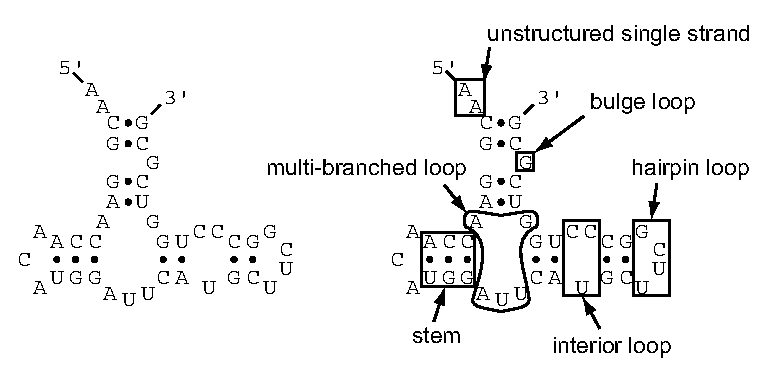
\includegraphics[scale=0.8]{figures/rna_elements}
\end{center}
\begin{center}
\begin{BVerbatim}
  ::((((,<<<___>>>,,,<<-<<____>>-->>,))-))
  AACGGAACCAACAUGGAUUCAUGCUUCGGCCCUGGUCGCG
\end{BVerbatim}
\end{center}

\subsection{Full (output) WUSS notation}

In detail, symbols used by WUSS notation in \emph{output} structure
annotation strings are as follows:

\begin{sreitems}{\textbf{Bulge, interior loops}}
\item[\textbf{Base pairs}]
  Base pairs are annotated by nested matching pairs of symbols
  \verb+<>+, \verb+()+, \verb+[]+, or \verb+{}+.
  The different symbols indicate the ``depth'' of the
  helix in the RNA structure as follows:
  \verb+<>+ are used for simple terminal stems;
  \verb+()+ are used for ``internal'' helices enclosing a multifurcation of
  all terminal stems; \verb+[]+ are used for internal helices
  enclosing a multifurcation that includes at least one annotated
  \verb+()+ stem already; and \verb+{}+ are used for all internal
  helices enclosing deeper multifurcations.

\item[\textbf{Hairpin loops}]
  Hairpin loop residues are indicated by underscores, \verb+_+.
  Simple stem loops stand out as, e.g.\ \verb+<<<<____>>>>+.

\item[\textbf{Bulge, interior loops}]
  Bulge and interior loop residues are indicated by dashes, \verb+-+.

\item[\textbf{Multifurcation loops}]
  Multifurcation loop residues are indicated by commas, \verb+,+.
  The mnemonic is ``stem 1, stem2'', e.g.\ \verb+<<<___>>>,,<<<___>>>+.

\item[\textbf{External residues}]
  Unstructured single stranded residues completely outside the
  structure (unenclosed by any base pairs) are annotated by
  colons, \verb+:+.

\item[\textbf{Insertions}]
  Insertions relative to a known structure are indicated by periods,
  \verb+.+. Regions where local structural alignment was invoked,
  leaving regions of both target and query sequence unaligned,
  are indicated by tildes, \verb+~+. These symbols only appear in
  alignments of a known (query) structure annotation to a target
  sequence of unknown structure.

\item[\textbf{Pseudoknots}]
  WUSS notation allows pseudoknots to be annotated as pairs of
  upper case/lower case letters: for example,
  \verb+<<<<_AAAA____>>>>aaaa+ annotates a simple pseudoknot;
  additional pseudoknotted stems could be annotated by \verb+Bb+,
  \verb+Cc+, etc. 

  This is not a fully general notation. It is possible to come up with
  pseudoknotted structures that could not be represented with 26
  levels of nesting ($>$26th order pseudoknot, in the sense of
  \citep{RivasEddy99}). However, it is unlikely you will ever see one
  in nature. I believe the highest order pseudoknot known is the S1
  (alpha operon) pseudoknot, which is 3rd order.
\end{sreitems}

An example of WUSS notation for a complicated structure
(\emph{E. coli} RNase P) is shown in Figure~\ref{fig:RNaseP}.  An
example of WUSS notation for a local alignment of \emph{B. subtilis}
RNase P to \emph{E. coli} RNase P, illustrating the use of local
alignment annotation symbols, is in Figure~\ref{fig:bsu-alignment}.

\begin{figure}[tp]
\begin{center}
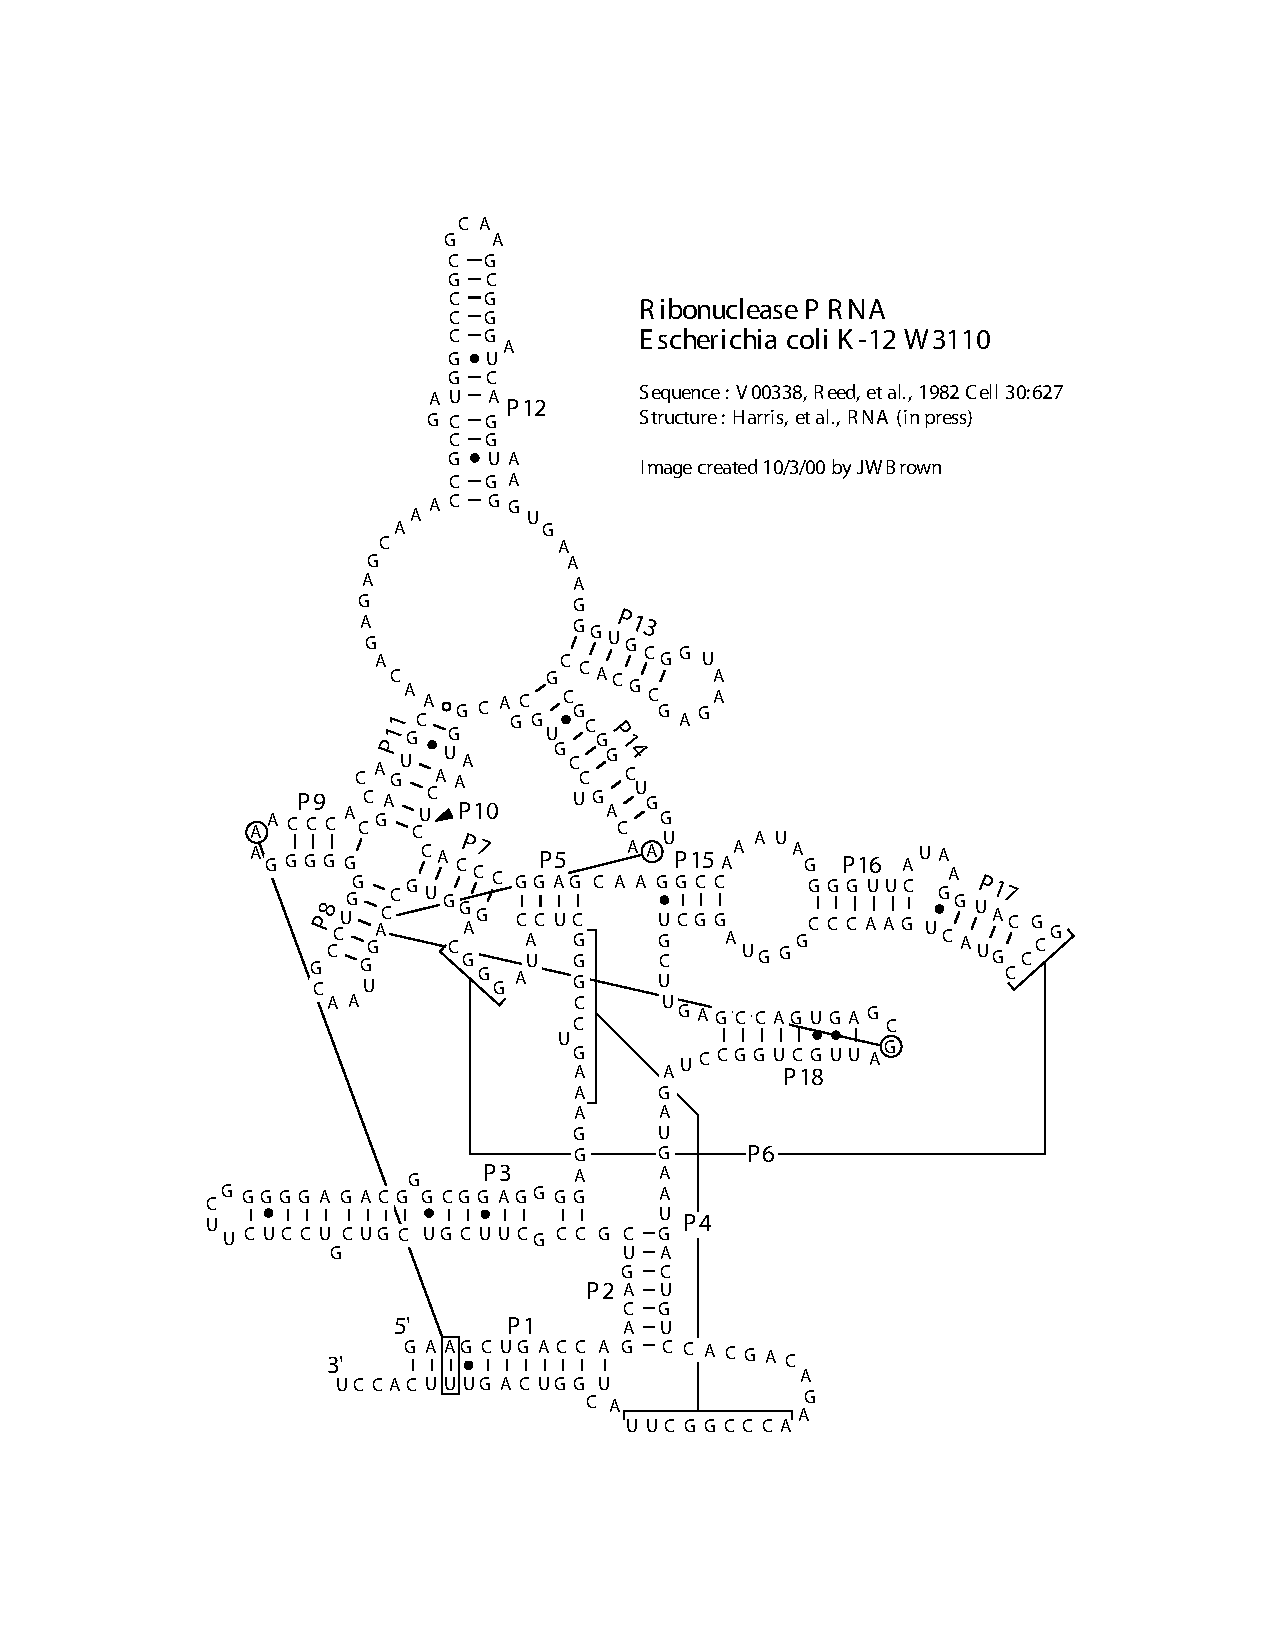
\includegraphics[scale=0.6]{figures/rnaseP-ecoli}
\end{center}
\begin{center}
{\scriptsize
\begin{BVerbatim}
           {{{{{{{{{{{{{{{{{{,<<<<<<<<<<<<<-<<<<<____>>>>>>>>>->>>>>>>>
         1 GAAGCUGACCAGACAGUCGCCGCUUCGUCGUCGUCCUCUUCGGGGGAGACGGGCGGAGGG 60

           >,,,,AAA-AAAAA[[[[---BBBB-[[[[[<<<<<_____>>>>><<<<____>>>->(
        61 GAGGAAAGUCCGGGCUCCAUAGGGCAGGGUGCCAGGUAACGCCUGGGGGGGAAACCCACG 120

           (---(((((,,,,,,,,,,,,<<<<<--<<<<<<<<____>>>>>->>>>>>-->>,,,,
       121 ACCAGUGCAACAGAGAGCAAACCGCCGAUGGCCCGCGCAAGCGGGAUCAGGUAAGGGUGA 180

           ,,,<<<<<<_______>>>>>><<<<<<<<<____>>>->>>>>->,,)))--))))]]]
       181 AAGGGUGCGGUAAGAGCGCACCGCGCGGCUGGUAACAGUCCGUGGCACGGUAAACUCCAC 240

           ]]]]]],,,<<<<------<<<<<<----<<<<<_bbbb>>>>>>>>>>>----->>>>,
       241 CCGGAGCAAGGCCAAAUAGGGGUUCAUAAGGUACGGCCCGUACUGAACCCGGGUAGGCUG 300

           ,,,,,<<<<<<<<____>>>>>>>>,,,,,,,,,,}}}}}}}----------aaaaaaaa
       301 CUUGAGCCAGUGAGCGAUUGCUGGCCUAGAUGAAUGACUGUCCACGACAGAACCCGGCUU 360

           -}-}}}}}}}}}}::::
       361 AUCGGUCAGUUUCACCU 377
\end{BVerbatim}
}
\end{center}
\caption{\small \textbf{Example of WUSS notation.} Top: Secondary
structure of \emph{E. coli} RNase P, from Jim Brown's RNase P database
\citep{Brown99}. Bottom: WUSS notation for the same structure,
annotating the \emph{E. coli} RNase P sequence. Note that the P4 and P6
pseudoknots are annotated, as A's and B's.}
\label{fig:RNaseP}
\end{figure}

\begin{figure}[tp]
\begin{center}
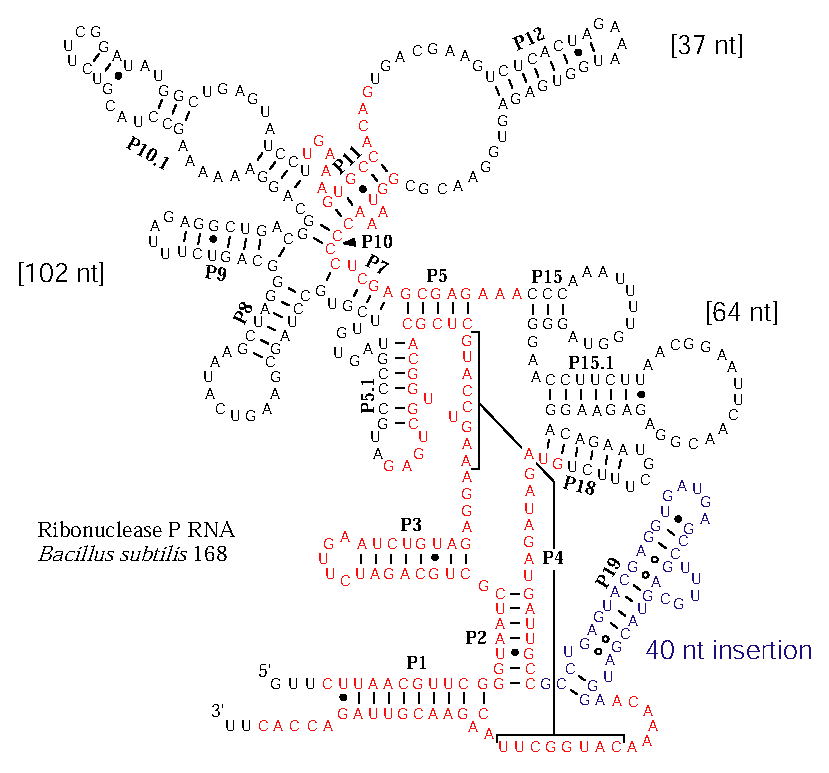
\includegraphics[scale=0.6]{figures/rnaseP-bsu-alignment}
\end{center}
\begin{center}
{\scriptsize
\begin{BVerbatim}
hit 0   :      4    399    52.56 bits
           {{{{{{{{{{{{{{{{{{,<<<<<<<<<<<<<-<<<<<____>>>>>>>>>->>>>>>>>
         1 ggAGuggGgcaGgCaguCGCugcuucggccuuGuucaguuaacugaaaaggAccgaagga 60
           +: :::G::C:GG:A:UCGCU+C::::            U+            ::::G+A
         4 CUUAACGUUCGGGUAAUCGCUGCAGAUC-----------UUG----------AAUCUGUA 42

           >,,,,,,,,,,,,,[[[.[--------[[[[[~~~~~~~((---(((((,,,,~~~~~~)
        61 GAGGAAAGUCCGGGCUC.CACAGGGCAgGGUG*[ 29]*GGAAAGUGCCACAG*[96]*G 229
           GAGGAAAGUCC  GCUC C  A GG   :G G       :GAAAGUGCCACAG      G
        43 GAGGAAAGUCCAUGCUCgC--ACGGUGCUGAG*[102]*UGAAAGUGCCACAG*[37]*G 226

           ))--))))]]]]]].]]],,,~~~~~~,,,,,,,,,,}}}}}}}--..............
       230 GUAAACCCCACCcG.GAGCAA*[77]*CuAGAUGAAUGacuGcCCA.............. 344
           GUAAACC:C C: G GAG AA       UAGAU++AUGA:U:CC
       227 GUAAACCCCUCGAGcGAGAAA*[64]*GUAGAUAGAUGAUUGCC--gccugaguacgagg 342

           ..........................-----------------}-}}}}}}}}}}::::
       345 ..........................CGACAGAACCCGGCUUAuagcCccaCUccucuu 377
                                       ACA AAC  GGCUUA:AG::C::: :+ C
       343 ugaugagccguuugcaguacgaugga--ACAAAACAUGGCUUACAGAACGUUAGACCAC 399
\end{BVerbatim}
}
\end{center}
\caption{\small \textbf{Local alignment annotation example.} Top:
Secondary structure of \emph{B. subtilis} RNase P, from Jim Brown's
RNase P database \citep{Brown99}. Residues in red are those that
Infernal aligns to a CM of \emph{E. coli} type RNase
P's. The local structural alignment is in four pieces; three regions
of the structure (102, 37, and 64 nt long) are skipped over. One
additional stem is treated as a 40 nt insertion. Bottom: the
Infernal output, showing the \emph{E. coli} query structure
aligned to the \emph{B. subtilis} sequence.}
\label{fig:bsu-alignment}
\end{figure}

\subsection{Shorthand (input) WUSS notation}

While WUSS notation makes it easier to visually interpret Infernal
\emph{output} structural annotation, it would be painful to require
people to \emph{input} all structures in full WUSS notation. Therefore
when software like Infernal reads input secondary structure
annotation, it also allows simpler rules:

\begin{sreitems}{\textbf{Single stranded residues}}
\item [\textbf{Base pairs}]
  Any matching nested pair of \verb+()+, \verb+()+, \verb+[]+, \verb+{}+
  symbols indicates a base pair; the exact choice of symbol has no
  meaning, so long as the left and right partners match up.
  Similarly, pseudoknotted pairs can also be annotated by matching nested
  pairs of any alphabet character, such as \verb+Aa+, \verb+Bb+, etc.

\item [\textbf{Single stranded residues}]
  All other symbols \verb+_-,:.~+
  indicate single stranded residues.
  The choice of symbol has no special meaning.
  Annotated pseudoknots (nested matched pairs of upper/lower case
  alphabetic characters) are also interpreted as single
  stranded residues in Infernal input.
\end{sreitems}

Thus, for instance, \verb+<<<<....>>>>+ and \verb+((((____))))+ and
\verb+<(<(._._)>)>+ all indicate a four base stem with a four base
loop (the last example is legal but weird).

Remember that the key property of canonical (nonpseudoknotted) RNA
secondary structure is that the pairs are \emph{nested}.
\verb+((<<....))>>+ is not a legal annotation string: the pair symbols
don't match up properly. 

Because many other RNA secondary structure analysis programs use a
simple bracket notation for annotating structure, the ability to input
the simple format makes it easier to use data generated by other RNA
software packages. Conversely, converting output WUSS notation to
simple bracket notation is a matter of a simple Perl or sed script,
substituting the symbols appropriately.



\newpage
\chapter{Developer's guide}

This chapter describes Easel from a developer's perspective. It shows
how a module's source code is organized, written, tested, and
documented. It should help you with implementing new Easel code, and
also with understanding the structure of existing Easel code.

We expect Easel to constantly evolve, both in code and in style.
Talking about our code style does not mean we enforce foolish
consistency. Rather, the goal is aspirational; one way we try to
manage the complexity of our growing codebase is to continuously
cajole Easel code toward a clean and consistent presentation. We try
to organize code modules in similar ways, use certain naming
conventions, and channel similar functions towards common
\esldef{interfaces} that provide common calling conventions and
behaviors.

But because it evolves, not all Easel code obeys the code style
described in this chapter. Easel code style is like a local building
ordinance. Any new construction should comply. Older construction is
grandfathered in and does not have to immediately conform to the
current rules. When it comes time to renovate, it's also time to bring
the old work up to the current standards.

For a concrete example we will focus primarily on one Easel module,
the \eslmod{buffer} module. We'll take a bottom up approach, starting
from the overall organization of the module and working down into
details. If you're a starting developer, you might have preferred a
bottom-up description; you might just want to know how to write or
improve a single Easel function, for example. In that case, skim
ahead.

%%%%%%%%%%%%%%%%%%%%%%%%%%%%%%%%%%%%%%%%%%%%%%%%%%%%%%%%%%%%%%%%
% Table: Easel naming conventions
%%%%%%%%%%%%%%%%%%%%%%%%%%%%%%%%%%%%%%%%%%%%%%%%%%%%%%%%%%%%%%%%
\begin{table}
\begin{minipage}{\textwidth}
\begin{tabular}{l>{\raggedright}p{3.5in}l}
\textbf{What}        & \textbf{Explanation}              & \textbf{Example} \\ \hline
Easel module
  &
    Module names should be 10 characters or less.\footnote{sqc assumes
    this in output formatting, for example.}
    Many modules are organized around a single Easel object
    that they implement. The name of the module matches the
    name of the object. For example, \ccode{esl\_buffer.c} implements \ccode{ESL\_BUFFER}.
  & \eslmod{buffer} \\ \\

tag name
  & Names in the module are constructed either using the module's full
    name or sometimes with a shorter abbreviation, usually 3
    characters (sometimes 2 or 4).
  & \ccode{buf} \\ \\

source file
  & Each module has one source file, named \ccode{esl\_}\itcode{modulename}\ccode{.c}.
  & \ccode{esl\_buffer.c} \\ \\

header file
  & Each module has one header file, named \ccode{esl\_}\itcode{modulename}\ccode{.h}.
  & \ccode{esl\_buffer.h} \\  \\

documentation 
  & Each module has one documentation chapter, named \ccode{esl\_}\itcode{modulename}\ccode{.tex}.
  & \ccode{esl\_buffer.tex} \\ \\

Easel object          
  & Easel ``objects'' are typedef'ed C structures (usually) or
    types (rarely\footnote{\ccode{ESL\_DSQ} is a \ccode{uint8\_t}, for example.}).
  & \ccode{ESL\_BUFFER} \\ \\  

external function 
  & All exposed functions have tripartite names \ccode{esl\_}\itcode{module}\ccode{\_specificname}().
    The specific part of function names often adhere to a standardized API
    ``interface'' nomenclature. (All \ccode{\_Open()} functions must follow the same standardized
    behavior guidelines, for example.) Functions in the base \ccode{easel.c} module
    have a bipartite name, omitting the module name. The specific 
    name part generally uses mixed case capitalization.
  & \ccode{esl\_buffer\_OpenFile()} \\ \\

static function 
  & Internal functions (static within a module file) drop the
    \ccode{esl\_} prefix, and are 
    named \itcode{modulename}\ccode{\_function}.
  & \ccode{buffer\_refill()} \\ \\

macro 
  & Macros follow the same naming convention as external functions,
    except they are all upper case.
  & \ccode{ESL\_ALLOC()} \\ \\ 

defined constant
  & Defined constants in Easel modules are named
    \ccode{esl}\itcode{MODULENAME}\ccode{\_FOO}. Constants defined
    in the base \ccode{easel.h} module are named just 
    \ccode{eslFOO}.
   & \ccode{eslBUFFER\_SLURPSIZE}\\ \\

return codes
  & Return codes are constants defined in \ccode{easel.h}, so 
    they obey the rules of other defined constants in the base module (\ccode{eslOK},
    \ccode{eslFAIL}). Additionally, error codes start with
    \ccode{E}, as in \ccode{eslE}\itcode{ERRTYPE}.
  & \ccode{eslENOTFOUND} \\ \\

config constant
  & Constants that don't start with \ccode{esl} are almost always 
    configuration (compile-time) constants determined by the autoconf
    \ccode{./configure} script and defined in \ccode{esl\_config.h}.
  & \ccode{HAVE\_STDINT\_H} \\ \\
\end{tabular}
\end{minipage}
\caption{\textbf{Easel naming conventions.} }
\end{table}



%%%%%%%%%%%%%%%%%%%%%%%%%%%%%%%%%%%%%%%%%%%%%%%%%%%%%%%%%%%%%%%%
\section{An Easel module}
%%%%%%%%%%%%%%%%%%%%%%%%%%%%%%%%%%%%%%%%%%%%%%%%%%%%%%%%%%%%%%%%

Each module consists of three files: a .c C code file, a .h header
file, and a .tex documentation file. These filenames are constructed
from the module name. For example, the \eslmod{buffer} module is
implemented in \ccode{esl\_buffer.c}, \ccode{esl\_buffer.h}, and
\ccode{esl\_buffer.tex}.

%%%%%%%%%%%%%%%%
\subsection{The .c file}
%%%%%%%%%%%%%%%%

Easel \ccode{.c} files are larger than most coding styles would
advocate. Easel module code is designed to be \emph{read}, to be
\emph{self-documenting}, to contain its own \emph{testing methods},
and to provide useful \emph{working examples}.  Thus the size of the
files is a little deceptive, compared to C code that's solely
implementating some functions. In general, only about a a quarter of
an Easel module's \ccode{.c} file is the actual module implementation.
Typically, around half of an Easel \ccode{.c} file is documentation,
and much of this gets automatically parsed into the PDF userguide. The
rest consists of drivers for unit testing and examples.

Module files are organized into a somewhat stereotypical set of
sections, to facilitate navigating the code, as follows.

The \ccode{.c} file starts with a comment that contains the {\bfseries
  table of contents}. The table of contents helps us navigate a long
Easel source file. This initial comment also includes a short
description of the module's purpose. It may also contain miscellaneous
notes.

For example, from the \eslmod{buffer} module:

\input{cexcerpts/header_example}

None of this is parsed automatically. Its structure is just
convention.

The short description lines in the table of contents match section
headings in comments later in the file. A search forward with the text
of a heading will move you to that section of the code.

Next come the {\bfseries includes} and any {\bf definitions}. Of the
include files, the \ccode{esl\_config.h} header must always be
included first. It contains platform-independent configuration code
that may affect even the standard library header files. Standard
headers like \ccode{stdio.h} come next, then Easel's main header
\ccode{easel.h}; then headers of any other Easel modules this module
depends on; then any headers for modules this module can be augmented
with, surrounded by appropriate \ccode{\#ifdef}'s; then the module's
own header. For example, the \ccode{\#include}'s in the
\eslmod{buffer} module look like:

\input{cexcerpts/include_example}

Next come the {\bfseries private function declarations}.  We declare
all private functions at the top of the file, where they can be seen
easily by a developer who's casually reading the source. Their
definitions are buried deeper, in one or more sections following the
implementation of the exposed API.

\input{cexcerpts/statics_example}

The rest of the file is the {\bfseries code}. It is split into
sections. Each section is numbered and given one-line titles that
appear in the table of contents.  Each section starts with a section
header, a comment block in front of each code section in the
\ccode{.c} file.  These section headers match comments in front of
that section's declarations in the \ccode{.h} file. Because of the
numbering and titling, a particular section of code can be located by
searching on the number or title.  A common section structure includes
the following, in this order:


\begin{description}
\item[\textbf{The \ccode{FOOBAR} object.}]
  The first section of the file provides the API for creating and
  destroying the object that this module implements.

\item[\textbf{The rest of the API.}]
  Everything else that is part of the API for this module in its
  baseline (unaugmented) form. This might be split across multiple
  sections.

\item[\textbf{Augmented API, if any.}]
  Any functions that are only available with one or more augmentations
  are split out into one or more separate sections. 

\item[\textbf{Debugging/dev code.}]
  Most objects can be validated or dumped to an output stream
  for inspection.

\item[\textbf{Private functions.}]
  Easel isn't rigorous about where private (non-exposed) functions go,
  but they often go in a separate section in about the middle of the
  \ccode{.c} file, after the API and before the drivers.

\item[\textbf{Optional drivers}] Stats, benchmark, and regression
  drivers, if any. 

\item [\textbf{Unit tests.}]
  The unit tests are internal controls that test that the module's API
  works as advertised.

\item [\textbf{Test driver.}]
  All modules have an automated test driver is a \ccode{main()} that
  runs the unit tests.
 
\item [\textbf{Examples.}]
  All modules have at least one \ccode{main()} showing an example of
  how to use the main features of the module.

\item [\textbf{Copyright/license information.}]  Each file ends with a
  \ccode{@LICENSE@} tag. This placeholder is automatically replaced by
  the correct license statement at packaging time. This gives us the
  ability to package specially licensed versions, in addition to the
  usual open source version. Automatically generated Subversion
  \ccode{SVN \$Id\$} and \ccode{SVN \$URL\$} information often appears
  here too.

\end{description}

%%%%%%%%%%%%%%%%
\subsection{The .h file}
%%%%%%%%%%%%%%%%


%%%%%%%%%%%%%%%%
\subsection{Special syntax in Easel C comments}
%%%%%%%%%%%%%%%%

Easel comments sometimes include special syntax recognized by tools other
than the compiler.  Here are some quick explanations of the special
stuff a developer needs to be aware of. 

\begin{table}
\begin{tabular}{l>{\raggedright}p{3.5in}l}
\textbf{Special syntax}  & \textbf{Description}  & \textbf{Parsed by}\\ \hline

\ccode{/* Function: }\itcode{funcname} 
  & Function documentation that gets converted to \LaTeX\ and included
    in Easel's PDF documentation.
  & \emcode{autodoc} \\ \\

\ccode{ *\# }\itcode{x.\ secheading} 
  & Section heading corresponding to section number x in a \ccode{.c}
    file's table of contents. This is automatically extracted as part
    of creating a summary table in the PDF documentation.
  & \emcode{autodoc -t} \\ \\

\ccode{/*::cexcerpt::} ...
  & Comments that marking beginning/end of code that is extracted
    verbatim into the documentation.
  & \emcode{cexcerpt} \\ \\

\ccode{ \$}\itcode{keyword}\ccode{\$} 
  & Subversion keyword substitutions
  & \emcode{svn} \\ \\

\ccode{@}\itcode{keyword}\ccode{@}
  & Configuration variable substitution
  & \emcode{sedition} \\ \\
\hline
\end{tabular}
\caption{{\bfseries Summary of special syntax in Easel C comments.}}
\end{table}

%%%%
\subsubsection{function documentation}
%%%%

Any comment that starts with
\begin{cchunk}
/* Function:  ...
\end{cchunk}
will be recognized and parsed by our \prog{autodoc} program, 
which assumes it is looking at a structured function documentation
header.

See section XX for details on how these headers work.

We want all external functions in the Easel API to be documented
automatically by \prog{autodoc}. We don't want internal functions tp
appear in the documentation, but we do want them documented in the
code.  To keep \prog{autodoc} from recognizing the function header of
an internal (static) function, we just leave off the \ccode{Function:}
tag in the comment block.   

%%%%
\subsubsection{section headings}
%%%%

The automatically generated \LaTeX\ code for a module's documentation
includes a table summarizing the functions in the exposed API. This
table is constructed automatically from the source code by
\prog{autodoc -t}. The list of functions in this table is extracted
from the function documentation (above). The table is broken into
sections, just as the module code is, using section headings. The
comment block marking the start of a section heading for exposed API
code has an extra \ccode{\#}:

\begin{cchunk}
/*****************************************************************
 *# 1. ESL_BUFFER object: opening/closing.
 *****************************************************************/
\end{cchunk}

Section headings for internal functions omit the \ccode{\#}, and
\prog{autodoc} ignores them:

\begin{cchunk}
/*****************************************************************
 * 10. Unit tests
 *****************************************************************/
\end{cchunk}

%%%%
\subsubsection{excerpting}
%%%%

This book includes many examples of C code extracted verbatim from
Easel source.  These {\bfseries excerpts} are marked with specially
formatted comments in the C file:

\begin{cchunk}
/*::cexcerpt::my_example::begin::*/
   while (esl_sq_Read(sqfp, sq) == eslOK)
     { n++; }
/*::cexcerpt::my_example::end::*/
\end{cchunk}

When we build the Easel documentation from its source, our
\prog{cexcerpt} program extracts all marked excerpts from \ccode{.c}
and \ccode{.h} files, and places them in individual files in a
temporary \ccode{cexcerpts/} directory, from where they are included
in the main \LaTeX documentation.

%%%%
\subsubsection{subversion keyword substitution (\$\$)}
%%%%

Comment lines containing Subversion \ccode{Id} and \ccode{URL}
keywords appear in the table of contents section:

\begin{cchunk}
 * SVN $Id: esl_buffer.c 662 2011-02-22 16:33:08Z eddys $
 * SVN $URL: https://svn.janelia.org/eddylab/eddys/easel/trunk/esl_buffer.c $
\end{cchunk}

These started out as
\begin{cchunk}
 * SVN $Id$
 * SVN $URL$
\end{cchunk}

and their contents get substituted by Subversion, our revision control
system.

If you add a new file to Easel and it has Subversion keywords in it,
you have to manually activate keyword substitution. 

\user{svn propset svn:keywords "Id URL" }\itbfcode{myfile}

%%%%
\subsubsection{configuration variable substitution (@@)}
%%%%

At the bottom of every source file is a comment block:

\begin{cchunk}
/*****************************************************************
 * @LICENSE@
 *****************************************************************/
\end{cchunk}

When we build a distribution package, the \ccode{@LICENSE@} tag is
replaced with by the appropriate copyright and license text by our
\prog{sedition} program. The command line appears in
\ccode{Makefile.in} in its \ccode{make dist}; it directs
\prog{sedition} to replace \ccode{@LICENSE@} tags with the contents of
the \ccode{LICENSE.tag} file (which is itself constructed
automatically at \ccode{make dist} time).

For example, the standard Easel release uses the Janelia Software
License (functionally identical to the BSDL), so in distribution code
this comment block something like:

\begin{cchunk}
/*****************************************************************
 * Easel - a library of C functions for biological sequence analysis
 * Version 0.42; February 2011
 * Copyright (C) 2011 Howard Hughes Medical Institute
 * Other copyrights also apply. See the COPYRIGHT file for a full list.
 *
 * Easel is distributed under the Janelia Farm Software License, a BSD
 * license. See the LICENSE file for more details.
 *****************************************************************/
\end{cchunk}

Autogenerating these license tags allows us to package distributions
under other licenses without having to edit every source file.

\ccode{@LICENSE@} is the only configuration variable that Easel
\ccode{.c} or \ccode{.h} files currently use. It's possible we would
add others in the future.


%%%%%%%%%%%%%%%%
\subsection{Driver programs}
%%%%%%%%%%%%%%%%

An unusual (innovative?) thing about Easel modules is how we embed
{\bfseries driver programs} directly in the module's \ccode{.c}
file. Driver programs include our unit tests, benchmarks, and working
examples. These small programs are enclosed in standardized
\ccode{\#ifdef}'s that enable them to be conditionally compiled.

None of these programs are installed by \ccode{make install}.  Test
drivers are compiled as part of \ccode{make check}.  A \ccode{make
  dev} compiles all driver programs.

There are six main types of drivers used in Easel:

\begin{description} 

\item[\textbf{Unit test driver(s).}] (Mandatory.) Each module has one (and only one)
  \ccode{main()} that runs the unit tests and any other automated for
  the module. The test driver is compiled and run by the testsuite in
  \ccode{testsuite/testsuite.sqc} when one does a \ccode{make check}
  on the package. It is also run by several of the automated tools
  used in development, including the coverage (\ccode{gcov}) and
  memory (\ccode{valgrind}) tests. A test driver takes no arguments
  (it must generate any input files it needs). If it succeeds, it
  returns 0, with no output. If it fails, it returns nonzero and calls
  \ccode{esl\_fatal()} to issue a short error message on
  \ccode{stdout}. Our test harness, \emcode{sqc}, depends on these
  output and exit status conventions. Optionally, it may use a flag
  to show more useful output when it's run more interactively.
  (usually a \ccode{-v}, for verbose).
  The test driver is enclosed by
  \ccode{\#ifdef esl}\itcode{MODULE}\ccode{\_TESTDRIVE} for
  conditional compilation.

\item[\textbf{Regression/comparison test(s).}] (Optional.) These tests
  link to one or more libraries that provide identical comparable
  functionality, such as previous versions of Easel, the old
  \prog{SQUID} library, \prog{LAPACK} or the GNU Scientific Library.
  They test that Easel's functionality performs at least as it used
  to, or as well as the 'competition'. These tests are run on demand,
  and not included in automated testing, because the other libraries
  may only be present on a subset of our development machines. They
  are enclosed by \ccode{\#ifdef
    esl}\itcode{MODULE}\ccode{\_REGRESSION} for conditional
  compilation.

\item[\textbf{Benchmark(s).}] (Optional.) These tests run a
  standardized performance benchmark and collect time and/or memory
  statistics. They may generate output suitable for graphing. They are
  run on demand, not by automated tools. They typically use 
  \eslmod{stopwatch} for timing. They are enclosed by
  \ccode{\#ifdef esl}\itcode{MODULE}\ccode{\_BENCHMARK}  for
  conditional compilation.

\item[\textbf{Statistics generator(s).}] (Optional.) These tests collect
  statistics used to characterize the module's scientific performance,
  such as its accuracy at some task. They may generate graphing
  output. They are run on demand, not by automated tools. They are
  enclosed by \ccode{\#ifdef esl}\itcode{MODULE}\ccode{\_STATS}
  for conditional compilation.

\item[\textbf{Experiment(s).}] (Optional.) These are other reproducible
  experiments we've done on the module code, essentially the same as
  statistics generators. They are
  enclosed by \ccode{\#ifdef esl}\itcode{MODULE}\ccode{\_EXPERIMENT}
  for conditional compilation.

\item[\textbf{Example(s).}] (Mandatory). Every module has at least one example
  \ccode{main()} that provides a ``hello world'' level example of
  using the module's API. Examples are enclosed in \ccode{cexcerpt}
  tags for extraction and verbatim inclusion in the documentation.
  They are enclosed by \ccode{\#ifdef esl}\itcode{MODULE}\ccode{\_EXAMPLE} 
  for conditional compilation.
\end{description}  

All modules have at least one test driver and one example. Other tests
and examples are optional. When there is more than one \ccode{main()}
of a given type, the additional tags are numbered starting from 2: for
example, a module with three example \ccode{main()'s} would have three
tags for conditional compilation, \ccode{eslFOO\_EXAMPLE},
\ccode{eslFOO\_EXAMPLE2}, and \ccode{eslFOO\_EXAMPLE3}.

The format of the conditional compilation tags for all the drivers
(including test and example drivers) must be obeyed. Some test scripts
are scanning the .c files and identifying these tags
automatically. For instance, the driver compilation test identifies any
tag named
\ccode{esl}\itcode{MODULENAME}\ccode{\_\{TESTDRIVE,EXAMPLE,REGRESSION,BENCHMARK,STATS\}*}
and attempt to compile the code with that tag defined.

Which driver is compiled (if any) is controlled by conditional
compilation of the module's \ccode{.c} file with the appropriate
tag. For example, to compile and run the \eslmod{sqio} test driver as
a standalone module:

\begin{cchunk}
   %  gcc -g -Wall -I. -o esl_sqio_utest -DeslSQIO_TESTDRIVE esl_sqio.c easel.c -lm
   %  ./esl_sqio_utest
\end{cchunk}

or to compile and run it in full library configuration:

\begin{cchunk}
   %  gcc -g -Wall -I. -L. -o esl_sqio_utest -DeslSQIO_TESTDRIVE esl_sqio.c -leasel -lm
   %  ./esl_sqio_utest
\end{cchunk}


\begin{table}
\begin{tabular}{llll}
\textbf{Driver type}     &  \textbf{Compilation flag}                       & \textbf{Driver program name}                     & \textbf{Notes}\\ \hline
Unit test                &  \ccode{esl}\itcode{MODULE}\ccode{\_TESTDRIVE}   & \ccode{esl\_}\itcode{module}\ccode{\_utest}      & output and exit status standardized for \emcode{sqc}\\
Regression test          &  \ccode{esl}\itcode{MODULE}\ccode{\_REGRESSION}  & \ccode{esl\_}\itcode{module}\ccode{\_regression} & may require other libraries installed\\
Benchmark                &  \ccode{esl}\itcode{MODULE}\ccode{\_BENCHMARK}   & \ccode{esl\_}\itcode{module}\ccode{\_benchmark}  & \\
Statistics collection    &  \ccode{esl}\itcode{MODULE}\ccode{\_STATS}       & \ccode{esl\_}\itcode{module}\ccode{\_stats}      & \\
Experiment               &  \ccode{esl}\itcode{MODULE}\ccode{\_EXPERIMENT}  & \ccode{esl\_}\itcode{module}\ccode{\_experiment} & \\
Example                  &  \ccode{esl}\itcode{MODULE}\ccode{\_EXAMPLE}     & \ccode{esl\_}\itcode{module}\ccode{\_example}    & \\
\end{tabular}
\caption{{\bfseries Summary of types of driver programs in Easel.}}
\end{table}









%%%%%%%%%%%%%%%%%%%%%%%%%%%%%%%%%%%%%%%%%%%%%%%%%%%%%%%%%%%%%%%%
\section{Writing an Easel function}
%%%%%%%%%%%%%%%%%%%%%%%%%%%%%%%%%%%%%%%%%%%%%%%%%%%%%%%%%%%%%%%%


Documentation of functions, particularly in the structured comment
header that's parsed by the \emcode{autodoc} program, is described in
a different section of its own.

%%%%
\subsubsection{conventions for function names}
%%%%

Function names are tripartite, constructed as
\ccode{esl\_}\itcode{moduletag\_funcname}.  

The \itcode{moduletag} should generally be the module's full name;
sometimes (historically) it is an abbreviated tag name for the module
(such as \ccode{abc} for the \eslmod{alphabet} module); on occasion,
it is the name of an Easel object or datatype that has not yet budded
off into its own module. Long versus short \itcode{moduletag}'s are
sometimes used to indicate functions that operate directly on objects
via common interfaces, versus other functions in the exposed API. The
long form may indicate functions that obey a common interface, such as
\ccode{esl\_alphabet\_Create()}.\footnote{This is a clumsy C version
  of what C++ would do with namespaces, object methods, and
  constructors/destructors.} Miscellaneous exposed functions in the API
  of a module may be named by the three-letter short tag, such as
  \ccode{esl\_abc\_Digitize()}.

The function's \ccode{\{funcname\}} can be anything. Some names
are standard and indicate the use of a common {\bfseries interface}.
This part of the name is usually in mixed-case capitalization.

Only exposed (\ccode{extern}) functions must follow these rules. In
general, private (\ccode{static}) functions can have any
name. However, it's common in Easel for private functions to obey the
same naming conventions except without the \ccode{esl\_} prefix.

Sometimes essentially the same function must be provided for different
data types. In these cases one-letter prefixes are used to indicate
datatype:

\begin{tabular}{ll}
\ccode{C} & \ccode{char} type, or a standard C string \\
\ccode{X} & \ccode{ESL\_DSQ} type, or an Easel digitized sequence\\
\ccode{I} & \ccode{int} type \\
\ccode{F} & \ccode{float} type \\
\ccode{D} & \ccode{double} type \\
\end{tabular}

For example, \eslmod{vectorops} uses this convention heavily;
\ccode{esl\_vec\_FNorm()} normalizes a vector of floats and
\ccode{esl\_vec\_DNorm()} normalizes a vector of doubles.  A second
example is in \eslmod{randomseq}, which provides routines for shuffling
either text strings or digitized sequences, such as
\ccode{esl\_rsq\_CShuffle()} and \ccode{esl\_rsq\_XShuffle()}.

%%%%
\subsubsection{conventions for argument names}
%%%%

When using pointers in C, it can be hard to tell which arguments are
for input data (which are provided by the caller and will not be
modified), output data (which are created and returned by the
function), and modified data (which are both input and output).  

For output consisting of pointers to nonscalar types such as objects
or arrays, it also can be hard to distinguish when the caller is
supposed to provide pre-allocated storage for the result, versus the
storage being newly allocated by the function.\footnote{A common
strategy in C library design is to strive for \emph{no} allocation in
the library, so the caller is always responsible for explicit
alloc/free pairs. I feel this puts a tedious burden of allocation code
on an application.}

When functions return more than one kind of result, it is convenient
to make all the individual results optional, so the caller doesn't
have to deal with managing storage for results it isn't interested in.
In Easel, an optional result pointer is passed as \ccode{NULL} to
indicate a possible result is not wanted (and is not allocated, if
returning that result required new allocation).

Easel uses a prefix convention on pointer argument names to indicate
these situations:

\begin{table}[h]
\begin{center}
{\small
\begin{tabular}{cp{2.5in}p{3in}}
 \textbf{prefix} &  \textbf{argument type}                  & \textbf{allocation (if any):}\\
none           & If qualified as \ccode{const}, a pointer
                 to input data, not modified by the call. 
                 If unqualified, a pointer to data modified
                 by the call (it's both input and output). & by caller\\ 
\ccode{ret\_}  & Pointer to result.                        & in the function \\
\ccode{opt\_}  & Pointer to optional result.               
                 If non-\ccode{NULL}, result is obtained. & in the function \\
\end{tabular}
}
\end{center}
\end{table}



%%%%
\subsubsection{Return status}
%%%%

%%%%
\subsubsection{conventions for exception handling}
%%%%

Easel functions {\bfseries should never exit except through an Easel
  return code or through the Easel exception handler}. When you write
Easel code you must {\bfseries always} deal with the case when the
caller has registered a nonfatal exception handler, causing thrown
exceptions to return a nonzero code rather than exiting. The Easel
library is designed to be used in programs that can't just suddenly
crash out with an error message (such as a graphical user interface
environment), and programs that have specialized error handlers
because they don't even have access to a \ccode{stderr} stream on a
terminal (such as a UNIX daemon).

This means that Easel functions must clean up their memory and set
appropriate return status and return arguments, even in the case of
thrown exceptions.


%%%%
\subsubsection{Easel's idiomatic function structure}
%%%%

To deal with the above strictures of return status, returned
arguments, and exception handling and cleanup, most Easel functions
follow an idiomatic structure.  The following snippet illustrates the
key ideas:

\begin{cchunk}
1    int
2    esl_example_Hello(char *opt_hello, char *opt_len)
3    {
4      char *msg = NULL;
5      int   n;
6      int   status;

7      if ( (status = esl_strdup("hello world!\n", -1, &msg)) != eslOK) goto ERROR;
8      n = strlen(msg);

9      if (opt_hello) *opt_hello = msg; else free(msg);
10     if (opt_len)   *opt_len   = n;
11     return eslOK;

12  ERROR:
13     if (msg)        free(msg);
14     if (opt_hello) *opt_hello = NULL;
15     if (opt_n)     *opt_n     = 0;
16     return status;
17  }
\end{cchunk}

The stuff to notice here:

\begin{itemize}
\item[line 2:] The \ccode{opt\_hello} and \ccode{opt\_len} arguments
  are optional. The caller might want only one of them (or neither,
  but that would be weird). We're expecting calls like
  \ccode{esl\_example\_Hello(\&hello, \&n)},
  \ccode{esl\_example\_Hello(\&hello, NULL)}, or
  \ccode{esl\_example\_Hello(NULL, \&n)}.

\item[line 4:] Anything we allocate, we initialize its pointer to \ccode{NULL}. 
  Now, if an exception occurs and we have to break out of the function early,
  we can tell whether the allocation has already happened (and hence we need
  to clean up its memory), if the pointer has become non-\ccode{NULL}.

\item[line 6:] Most functions have an explicit \ccode{status} variable.
  Standard error-handling macros (\ccode{ESL\_XEXCEPTION()} for example) expect it to be present,
  as do standard allocation macros (\ccode{ESL\_ALLOC()} for example).
  If we have to handle an exception, we're going to make sure the status
  is set how we want it, then jump to a cleanup block.

\item[line 7:] When any Easel function calls another Easel function,
  it must check the return status for both normal errors and thrown
  exceptions. If an exception has already been thrown by a callee,
  usually the caller just relays the exception status up the call
  stack. The idiom is to set the return \ccode{status} and go
  immediately to the error cleanup block, \ccode{ERROR:}. We use a
  \ccode{goto} for this, Dijkstra notwithstanding.

\item[lines 9,10:] When we set optional arguments for a normal return,
  we first check whether a valid return pointer was provided. If the
  optional pointer is \ccode{NULL} the caller doesn't want the result,
  and we clean up any memory we need to (line 9).

\item[line 13:] In the error cleanup block, we first free any memory
  that got allocated before the failure point. The idiom of
  immediately initializing all allocated pointers to \ccode{NULL} 
  enables us to tell which things have been allocated or not.

\item[line 14:] When we return from a function with an unsuccessful 
  status, we also make sure that any returned arguments are in 
  a documented ground state, usually \ccode{NULL}'s and \ccode{0}'s.
\end{itemize}

%%%%
\subsubsection{reentrancy: plan for threads}
%%%%

Easel code must expect to be called in multithreaded applications. All
functions must be reentrant. There should be no use of global or
static variables. 





%%%%%%%%%%%%%%%%%%%%%%%%%%%%%%%%%%%%%%%%%%%%%%%%%%%%%%%%%%%%%%%%
\section{Standard Easel function interfaces}
%%%%%%%%%%%%%%%%%%%%%%%%%%%%%%%%%%%%%%%%%%%%%%%%%%%%%%%%%%%%%%%%

Some function names are shared and have common behaviors across
modules, like \ccode{\_Get*()} and \ccode{\_Set*()} functions.  These
special names are called \esldef{common interfaces}.

\begin{table}
\begin{minipage}{\textwidth}
\begin{tabular}{l>{\raggedright}p{3.0in}ll}
\textbf{Function name}        & \textbf{Description}              & \textbf{Returns} &  \textbf{Example} \\ \hline
 \multicolumn{4}{c}{\bfseries Creating and destroying new objects}\\
\ccode{\_Create}
  & Create a new object.
  & \ccode{ESL\_}\itcode{FOO}\ccode{ *}
  & \ccode{esl\_alphabet\_Create()} \\

\ccode{\_Destroy}
  & Free an object.
  & \ccode{void}
  & \ccode{esl\_alphabet\_Destroy()} \\

\ccode{\_Clone}
  & Duplicate an object, by creating and allocating a new one.
  & \ccode{ESL\_}\itcode{FOO}\ccode{ *}
  & \ccode{esl\_msa\_Clone()} \\

\ccode{\_Shadow}
  & Partially duplicate an object, creating a dependent shadow.
  & \ccode{ESL\_}\itcode{FOO}\ccode{ *}
  & \ccode{p7\_oprofile\_Shadow()} \\

\ccode{\_Copy}
  & Make a copy of an object, using an existing allocated object for space.
  & [standard]
  & \ccode{esl\_msa\_Copy()} \\

 \multicolumn{4}{c}{\bfseries Opening and closing input sources}\\
\ccode{\_Open} 
  & Open an input source, associating it with an Easel object. 
  & [standard]
  & \ccode{esl\_buffer\_Open()} \\

\ccode{\_Close}
  & Close an Easel object corresponding to an input source.
  & [standard]
  & \ccode{esl\_buffer\_Close()} \\

 \multicolumn{4}{c}{\bfseries Managing memory allocation}\\

\ccode{\_Grow}
  & Expand the allocation in an existing object, typically by doubling.
  & [standard]
  & \ccode{esl\_tree\_Grow()} \\

\ccode{\_GrowTo}
  & Reallocate object (if needed) for some new data size.
  & [standard]
  & \ccode{esl\_sq\_GrowTo()} \\

\ccode{\_Reuse}
  & Recycle an object, reinitializing it while reusing as much of its existing
    allocation(s) as possible.
  & [standard]
  & \ccode{esl\_keyhash\_Reuse()} \\

\ccode{size\_t \_Sizeof}
  & Return the allocation size of an object
  & size, in bytes
  & - \\



 \multicolumn{4}{c}{\bfseries Accessing information in objects}\\

\ccode{\_Is}
  & Return \ccode{TRUE} or \ccode{FALSE} for some query of the
    internal state of an object.
  & \ccode{TRUE | FALSE}
  & \ccode{esl\_opt\_IsOn()} \\

\ccode{\_Get}
  & Return a value for some query of the internal state of an object.
  & value
  & \ccode{esl\_buffer\_Get()} \\

\ccode{\_Read}
  & Get a value in the object and return it in a location provided (and possibly allocated) by the caller.
  & [standard]
  & \ccode{esl\_buffer\_Read()} \\

\ccode{\_Fetch}
  & Get a value in the object and return it in newly allocated space;
    the caller becomes responsible for the newly allocated space.
  & [standard]
  & \ccode{esl\_buffer\_FetchLine()} \\  

\ccode{\_Set}
  & Set a value in the object.
  & [standard]
  & \ccode{esl\_buffer\_Set()} \\

\ccode{\_Format}
  & Set a string in the object using \ccode{sprintf()}-like
    semantics.
  & [standard]
  & \ccode{esl\_msa\_FormatName()} \\



 \multicolumn{4}{c}{\bfseries Debugging}\\
\ccode{\_Validate}
  & Run validation tests on the internal state of an object.
  & [standard]
  & \ccode{esl\_tree\_Validate()} \\

\ccode{\_Compare}
  & Compare two objects to each other for equality (or close enough).
  & [standard]
  & \ccode{esl\_msa\_Compare()} \\

\ccode{\_Dump}
  & Dump a verbose, possibly ugly, but developer-readable output 
    of the internal state of an object.
  & [standard]
  & \ccode{esl\_keyhash\_Dump()} \\

\ccode{\_TestSample}
  & Sample a mostly syntactically correct object for test purposes
  & [standard]
  & \ccode{p7\_tophits\_TestSample()} \\



 \multicolumn{4}{c}{\bfseries Miscellaneous}\\

\ccode{\_Write}
  & Write something from an object to an output stream.
  & [standard]
  & \ccode{esl\_msa\_Write()} \\

\ccode{\_Encode}
  & Convert a user-readable string (such as ``fasta'') to an
    internal Easel code (such as \ccode{eslSQFILE\_FASTA}).
  & [standard]
  & \ccode{esl\_msa\_EncodeFormat()} \\

\ccode{\_Decode}
  & Convert an internal Easel code (such as \ccode{eslSQFILE\_FASTA}) 
    to a user-readable string (such as ``fasta'').
  & [standard]
  & \ccode{esl\_msa\_DecodeFormat()} \\
\end{tabular}
\end{minipage}
\caption{\textbf{Standard function ``interfaces''.} }
\end{table}


%%%%%%%%%%%%%%%%
\subsection{Creating and destroying new objects}
%%%%%%%%%%%%%%%%

Most Easel objects are allocated and free'd by
\ccode{\_Create()/\_Destroy()} interface. Creating an object often
just means allocating space for it, so that some other routine can
fill data into it. It does not necessarily mean that the object
contains valid data.

\begin{sreapi}


\hypertarget{ifc:Create} 
{\item[\_Create(n)]}

A \ccode{\_Create()} interface takes any necessary initialization or
size information as arguments (there often aren't any), and it returns a
pointer to the newly allocated object. If an (optional) number of
elements \ccode{n} is provided, this specifies the number of elements
that the object is going to contain (for a fixed-size object) or the
initial allocation size (for a resizable object). In the event of an
allocation failure, a \ccode{\_Create} procedure throws \ccode{NULL}.

(If any error other than an allocation failure can happen, you should
use \ccode{\_Build()} instead. A caller is allowed to assume that a
\ccode{NULL} return from \ccode{\_Create()} is equivalent to
\ccode{eslEMEM}.)

The internals of some resizeable objects have an \ccode{nredline}
parameter that controls an additional memory management rule. These
objects are allowed to grow to arbitrary size (either by doubling with
\ccode{\_Grow} or by a specific allocation with \ccode{\_Reinit} or
\ccode{\_GrowTo}) -- but when the object is reused for new data, they
can be reallocated \emph{downward}, back to the redline
limit. Specifically, if the allocation size exceeds \ccode{nredline},
a \ccode{\_Reuse()} or \ccode{\_Reinit()} call will shrink the
allocation back to the \ccode{nredline} limit.  The idea is for a
frequently-reused object to be able to briefly handle a rare
exceptionally large problem, while not permanently committing the
resizeable object to an extreme allocation size.

At least one module (\ccode{esl\_tree}) allows for creating either a
fixed-size or a resizeable object; in this case, there is a
\ccode{\_CreateGrowable()} call for the resizeable version.




\hypertarget{ifc:Build} 
{\item[\_Build()]}

A \ccode{\_Build()} interface is the same as \ccode{\_Create()}, but
instead of returning a pointer to the new object, we return an Easel
error code, and the new object is returned through a \ccode{*ret\_obj}
argument.





\hypertarget{ifc:Destroy} 
{\item[\_Destroy(obj)]}
A \ccode{\_Destroy()} interface takes an object pointer as an
argument, and frees all the memory associated with it. A
\ccode{\_Destroy} procedure returns \ccode{void} (there is no useful
information to return about a failure; the only calls are to 
\ccode{free()} and if that fails, we're in trouble).
\end{sreapi}

For example:
\begin{cchunk}
   ESL_SQ *sq;
   sq = esl_sq_Create();
   esl_sq_Destroy(sq);
\end{cchunk}




%%%%%%%%%%%%%%%%
  \subsubsection{opening and closing input streams}
%%%%%%%%%%%%%%%%

Some objects (such as \ccode{ESL\_SQFILE} and \ccode{ESL\_MSAFILE})
correspond to open input streams -- usually an open file, but possibly
reading from a pipe. Such objects are \ccode{\_Open()}'ed and
\ccode{\_Close()'d}, not created and destroyed.

Input stream objects have to be capable of handling normal failures,
because of bad user input. Input stream objects contain an
\ccode{errbuf[eslERRBUFSIZE]} field to capture informative parse error
messages. 

\begin{sreapi}
\hypertarget{ifc:Open} 
{\item[\_Open(file, formatcode, \&ret\_obj)]}

Opens the \ccode{file}, which is in a format indicated by
\ccode{formatcode} for reading; return the open input object in
\ccode{ret\_obj}. A \ccode{formatcode} of 0 typically means unknown,
in which case the \ccode{\_Open()} procedure attempts to autodetect
the format. If the \ccode{file} is \ccode{"-"}, the object is
configured to read from the \ccode{stdin} stream instead of opening a
file. If the \ccode{file} ends in a \ccode{.gz} suffix, the object is
configured to read from a pipe from \ccode{gzip -dc}. Returns
\ccode{eslENOTFOUND} if \ccode{file} cannot be opened, and
\ccode{eslEFORMAT} if autodetection is attempted but the format cannot
be determined. 

Newer \ccode{\_Open} procedures return a standard Easel error code,
and on a normal error they also return the allocated object, using the
object's error message buffer to report the reason for the failed
open.

\hypertarget{ifc:Close} 
{\item[\_Close(obj)]}

Closes the input stream \ccode{obj}. Should return a standard Easel
error code. There are cases where an error in an input stream is only
detected at closing time (inputs using \ccode{popen()}/\ccode{pclose()}
  are an example).
\end{sreapi}

For example:
\begin{cchunk}
    char        *seqfile = "foo.fa";
    ESL_SQFILE  *sqfp;

    esl_sqio_Open(seqfile, eslSQFILE_FASTA, NULL, &sqfp);
    esl_sqio_Close(sqfp);
\end{cchunk}


%%%%
  \subsubsection{making copies of objects}
%%%%

\begin{sreapi}

\hypertarget{ifc:Clone}
{\item[\_Clone(obj)]}

Creates and returns a pointer to a duplicate of \ccode{obj}.
Equivalent to (and is a shortcut for, and is generally implemented as)
\ccode{dest = \_Create(); \_Copy(src, dest)}. Caller is responsible
for free'ing the duplicate object, just as if it had been
\ccode{\_Create}'d. Throws \ccode{NULL} if allocation fails.


\hypertarget{ifc:Copy}
{\item[\_Copy(src, dest)]}

Copies \ccode{src} object into \ccode{dest}, where the caller has
already created an appropriately allocated and empty \ccode{dest}
object (or buffer, or whatever). Returns \ccode{eslOK} on success;
throws \ccode{eslEINCOMPAT} if the objects are not compatible (for
example, two matrices that are not the same size).

Note that the order of the arguments is always \ccode{src}
$\rightarrow$ \ccode{dest} (unlike the C library's \ccode{strcpy()}
convention, which is the opposite order).


\hypertarget{ifc:Shadow}
{\item[\_Shadow(obj)]}

Creates and returns a pointer to a partial, dependent copy of
\ccode{obj}. Shadow creation arises in multithreading, when threads
can share some but not all internal object data. A shadow keeps
constant data as pointers to the original object.  The object needs to
know whether it is a shadow or not, so that <_Destroy()> works
properly on both the original and its shadows.

\end{sreapi}

%%%%%%%%%%%%%%%%
  \subsection{Managing memory allocation}
%%%%%%%%%%%%%%%%

%%%%
  \subsubsection{resizable objects}
%%%%

Some objects need to be reallocated and expanded during their use.
These objects are called \esldef{resizable}.

In some cases, the whole purpose of the object is to have elements
added to it, such as \ccode{ESL\_STACK} (pushdown stacks) and
\ccode{ESL\_HISTOGRAM} (histograms). In these cases, the normal
\ccode{\_Create()} interface performs an initial allocation, and the
object keeps track of both its current contents size (often
\ccode{obj->N}) and the current allocation size (often
\ccode{obj->nalloc}). 

In at least one case, an object might be either growable or not,
depending on how it's being used. This happens, for instance, when we
have routines for parsing input data to create a new object, and we
need to dynamically reallocate as we go because the input doesn't tell
us the total size when we start. For instance, with \ccode{ESL\_TREE}
(phylogenetic trees), sometimes we know exactly the size of the tree
we need to create (because we're making a tree ourselves), and
sometimes we need to create a resizable object (because we're reading a
tree from a file). In these cases, the normal \ccode{\_Create()}
interface creates a static, nongrowable object of known size, and a
\ccode{\_CreateGrowable()} interface specifies an initial allocation
for a resizable object.

Easel usually handles its own reallocation of resizable objects. For
instance, many resizable objects have an interface called something
like \ccode{\_Add()} or \ccode{\_Push()} for storing the next element
in the object, and this interface will deal with increasing allocation
size as needed.  In a few cases, a public \ccode{\_Grow()} interface
is provided for reallocating an object to a larger size, in cases
where a caller might need to grow the object itself. \ccode{\_Grow()}
only increases an allocation when it is necessary, and it makes that
check immediately and efficiently, so that a caller can call
\ccode{\_Grow()} before every attempt to add a new element without
worrying about efficiency. An example of where a public
\ccode{\_Grow()} interface is generally provided is when an object
might be input from different file formats, and an application may
need to create its own parser. Although creating an input parser
requires familiarity with the Easel object's internal data structures,
at least the \ccode{\_Grow()} interface frees the caller from having
to understand its memory management.

Resizable objects necessarily waste some memory, because they are
overallocated in order to reduce the number of calls to
\ccode{malloc()}.  The wastage is bounded (to a maximum of two-fold,
for the default doubling strategies, once an object has exceeded its
initial allocation size) but nonetheless may not always be tolerable.

In summary: 

\begin{sreapi}
\hypertarget{ifc:Grow}
{\item[\_Grow(obj)]}

A \ccode{\_Grow()} function checks to see if \ccode{obj} can hold
another element. If not, it increases the allocation, according to
internally stored rules on reallocation strategy (usually, by
doubling). 
\end{sreapi}

\begin{sreapi}
\hypertarget{ifc:GrowTo}
{\item[\_GrowTo(obj, n)]}

A \ccode{\_GrowTo()} function checks to see \ccode{obj} is large
enough to hold \ccode{n} elements. If not, it reallocates to at least
that size.
\end{sreapi}

%%%%
  \subsubsection{reusable objects}
%%%%

Memory allocation is computationally expensive. An application needs
to minimize \ccode{malloc()/free()} calls in performance-critical
regions. In loops where one \ccode{\_Destroy()}'s an old object only
to \ccode{\_Create()} the next one, such as a sequential input loop
that processes objects from a file one at a time, one generally wants
to \ccode{\_Reuse()} the same object instead:

\begin{sreapi}
\hypertarget{ifc:Reuse}
{\item[\_Reuse(obj)]}

A \ccode{\_Reuse()} interface takes an existing object and
reinitializes it as a new object, while reusing as much memory as
possible. Any state information that was specific to the problem the
object was just used for is reinitialized. Any allocations and state
information specific to those allocations are preserved (to the extent
possible).  A \ccode{\_Reuse()} call should exactly replace (and be
equivalent to) a \ccode{\_Destroy()/\_Create()} pair. If the object is
growable, it typically would keep the last allocation size, and it
must keep at least the same allocation size that a default
\ccode{\_Create()} call would give.

If the object is arbitrarily resizeable and it has a \ccode{nredline}
control on its memory, the allocation is shrunk back to
\ccode{nredline} (which must be at least the default initial
allocation).

\end{sreapi}

For example:

\begin{cchunk}
   ESL_SQFILE *sqfp;
   ESL_SQ     *sq;

   esl_sqfile_Open(\"foo.fa\", eslSQFILE_FASTA, NULL, &sqfp);
   sq = esl_sq_Create();
   while (esl_sqio_Read(sqfp, sq) == eslOK)
    {
       /* do stuff with this sq */
       esl_sq_Reuse(sq);
    }
   esl_sq_Destroy(sq);
\end{cchunk}

%%%%
  \subsubsection{other}
%%%%
\begin{sreapi}
\hypertarget{ifc:Sizeof}
{\item[size\_t \_Sizeof(obj)]}

Returns the total size of an object and its allocations, in bytes.
\end{sreapi}


%%%%%%%%%%%%%%%%
 \subsection{Accessing information in objects}
%%%%%%%%%%%%%%%%

\begin{sreapi}

\hypertarget{ifc:Is}
{\item[\_Is*(obj)]}

Performs some specific test of the internal state of an
object, and returns \ccode{TRUE} or \ccode{FALSE}.

\hypertarget{ifc:Get}
{\item[value = \_Get*(obj, ...)]}

Retrieves some specified data from \ccode{obj} and returns it
directly. Because no error code can be returned, a \ccode{\_Get}
call must be a simple access call within the object, guaranteed to
succeed. \ccode{\_Get()} methods may often be implemented as macros.
(\ccode{\_Read} or \ccode{\_Fetch} interfaces are for more complex
access methods that might fail, and require an error code return.)

\hypertarget{ifc:Read}
{\item[\_Read*(obj, ..., \&ret\_value)]}

Retrieves some specified data from \ccode{obj} and puts it in
\ccode{ret\_value}, where caller has provided (and already allocated,
if needed) the space for \ccode{ret\_value}.

\hypertarget{ifc:Fetch}
{\item[\_Fetch*(obj, ..., \&ret\_value)]}

Retrieves some specified data from \ccode{obj} and puts it in
\ccode{ret\_value}, where space for the returned value is allocated by
the function. Caller becomes responsible for free'ing that space.

\hypertarget{ifc:Set}
{\item[\_Set*(obj, value)]}

Sets some value(s) in \ccode{obj} to \ccode{value}. If a value was
already set, it is replaced with the new one. If any memory needs to
be reallocated or free'd, this is done. \ccode{\_Set} functions have
some appropriate longer name, like \ccode{\_SetZero()} (set something
in an object to zero(s)), or \ccode{esl\_dmatrix\_SetIdentity()} (set
a dmatrix to an identity matrix).

\hypertarget{ifc:Format}
{\item[\_Format*(obj, fmtstring, ...)]}

Like \ccode{\_Set}, but with \ccode{sprintf()}-style semantics.  Sets
some string value in \ccode{obj} according to the
\ccode{sprintf()}-style \ccode{fmtstring} and any subsequence
\ccode{sprintf()}-style arguments. If a value was already set, it is
replaced with the new one. If any memory needs to be reallocated or
free'd, this is done.  \ccode{\_Format} functions have some
appropriate longer name, like
\ccode{esl\_msa\_FormatSeqDescription()}.

Because \ccode{fmtstring} is a \ccode{printf()}-style format string,
it must not contain '\%' characters. \ccode{\_Format*} functions
should only be used with format strings set by a program; they should
not be used to copy user input that might contain '\%' characters.
\end{sreapi}


%%%%%%%%%%%%%%%%
\subsection{Debugging, testing, development}
%%%%%%%%%%%%%%%%

\begin{sreapi}
\hypertarget{ifc:Validate}
{\item[\_Validate*(obj, errbuf...)]}

Checks that the internals of \ccode{obj} are all right. Returns
\ccode{eslOK} if they are, and returns \ccode{eslFAIL} if they
aren't. Additionally, if the caller provides a non-\ccode{NULL}
message buffer \ccode{errbuf}, on failure, an informative message
describing the reason for the failure is formatted and left in
\ccode{errbuf}. If the caller provides this message buffer, it must
allocate it for at least \ccode{eslERRBUFSIZE} characters.

Failures in \ccode{\_Validate()} routines are handled by
\ccode{ESL\_FAIL()} (or \ccode{ESL\_XFAIL()}, if the validation
routine needs to do any memory cleanup).  Validation failures are
classified as normal (returned) errors so that \ccode{\_Validate()}
routines can be used in production code -- for example, to validate
user input.

At the same time, because the \ccode{ESL\_FAIL()} and
\ccode{ESL\_XFAIL()} macros call the stub \ccode{esl\_fail()}, you can
set a debugging breakpoint on \ccode{esl\_fail} to get a
\ccode{\_Validate()} routine fail immediately at whatever test
failed. 

The \ccode{errbuf} message therefore can be coarse-grained
(``validation of object X failed'') or fine-grained (``in object X,
data element Y fails test Z''). A validation of user input (which we
expect to fail often) should be fine-grained, to return maximally
useful information about what the user did wrong. A validation of
internal data can be very coarse-grained, knowing that a developer can
simply set a breakpoint in \ccode{esl\_fail()} to get at exactly where
a validation failed.

A \ccode{\_Validate()} function is not intended to test all possible
invalid states of an object, even if that were feasible. Rather, the
goal is to automatically catch future problems we've already seen in
past debugging and testing. So a \ccode{\_Validate()} function is a
place to systematically organize a set of checks that essentially
amount to regression tests against past debugging/testing efforts.

\hypertarget{ifc:Compare}
{\item[\_Compare*(obj1, obj2...)]}

Compares \ccode{obj1} to \ccode{obj2}. Returns \ccode{eslOK} if the
contents are judged to be identical, and \ccode{eslFAIL} if they
differ. When the comparison involves floating point scalar
comparisons, a fractional tolerance argument \ccode{tol} is also
passed. 

Failures in \ccode{\_Compare()} functions are handled by
\ccode{ESL\_FAIL()} (or \ccode{ESL\_XFAIL()}, if the validation
routine needs to do any memory cleanup), because they may be used in a
context where a ``failure'' is expected; for example, when using
\ccode{esl\_dmatrix\_Compare()} as a test for successful convergence
of a matrix algebra routine. 

However, the main use of \ccode{\_Compare()} functions is in unit
tests. During debugging and development, we want to see exactly where
a comparison failed, and we don't want to have to write a bunch
laboriously informative error messages to get that information.
Instead we can exploit the fact that the \ccode{ESL\_FAIL()} and
\ccode{ESL\_XFAIL()} macros call the stub \ccode{esl\_fail()}; you can
set a debugging breakpoint in \ccode{esl\_fail()} to stop execution in
the failure macros.

\hypertarget{ifc:Dump}
{\item[\_Dump*(FILE *fp, obj...)]}

Prints the internals of an object in human-readable, easily parsable
tabular ASCII form. Useful during debugging and development to view
the entire object at a glance. Returns \ccode{eslOK} on success.
Unlike a more robust \ccode{\_Write()} call, \ccode{\_Dump()} call may
assume that all its writes will succeed, and does not need to check
return status of \ccode{fprintf()} or other system calls, because it
is not intended for production use.


\hypertarget{ifc:TestSample}
{\item[\_TestSample(ESL\_RANDOMNESS *rng, ..., OBJTYPE **ret\_obj)]}

Create an object filled with randomly sampled values for all data
elements. The aim is to exercise valid values and ranges, and
presence/absence of optional information and allocations, but not to
obsess about internal semantic consistency. For example, we use
\ccode{\_TestSample()} calls in testing MPI send/receive
communications routines, where we don't care so much about the meaning
of the object's contents, as we do about faithful transmission of any
object with valid contents. 

A \ccode{\_TestSample()} call produces an object that is sufficiently
valid for other debugging tools, including \ccode{\_Dump()},
\ccode{\_Compare()}, and \ccode{\_Validate()}. However, because
elements may be randomly sampled independently, in ways that don't
respect interdependencies, the object may contain data inconsistencies
that make the object invalid for other purposes.  Contrast
\ccode{\_Sample()} routines, which generate fully valid objects for
all purposes, but which may not exercise the object's fields as
thoroughly.

\end{sreapi}

%%%%%%%%%%%%%%%%
\subsection{Miscellaneous other interfaces}
%%%%%%%%%%%%%%%%

\begin{sreapi}
\hypertarget{ifc:Write}
{\item[\_Write(fp, obj)]}
Writes something from an object to an output stream \ccode{fp}. Used
for exporting and saving files in official data exchange formats.
\ccode{\_Write()} functions must be robust to system write errors,
such as filling or unexpectedly disconnecting a disk. They must check
return status of all system calls, and throw an \ccode{eslEWRITE}
error on any failures.




\hypertarget{ifc:Encode}
{\item[code = \_Encode*(char *s)]}

Given a string \ccode{<s>}, match it case-insensitively against a list
of possible string values and convert this visible representation to
its internal \ccode{\#define} or \ccode{enum} code. For example,
\ccode{esl\_sqio\_EncodeFormat("fasta")} returns
\ccode{eslSQFILE\_FASTA}. If the string is not recognized, returns a
code signifying ``unknown''. This needs to be a normal return (not a
thrown error) because the string might come from user input, and might
be invalid.


\hypertarget{ifc:Decode}
{\item[char *s = \_Decode*(int code)]}

Given an internal code (an \ccode{enum} or \ccode{\#define} constant),
return a pointer to an informative string value, for diagnostics and
other output. The string is static. If the code is not recognized,
throws an \ccode{eslEINVAL} exception and returns \ccode{NULL}.

\end{sreapi}






%%%%%%%%%%%%%%%%%%%%%%%%%%%%%%%%%%%%%%%%%%%%%%%%%%%%%%%%%%%%%%%%
\section{Writing unit tests}
%%%%%%%%%%%%%%%%%%%%%%%%%%%%%%%%%%%%%%%%%%%%%%%%%%%%%%%%%%%%%%%%

An Easel test driver runs a set of individual unit tests one after
another.  Sometimes there is one unit test assigned to each exposed
function in the API. Sometimes, it makes sense to test several exposed
functions in a single unit test function.

A unit test for \ccode{esl\_foo\_Baz()} is named \ccode{static void
utest\_Baz()}. 

Upon success, unit tests return void.

Upon any failure, a unit test calls \ccode{esl\_fatal()} with an error
message, and terminates. It should not use any other error-catching
mechanism. It aids debugging if the test program terminates
immediately, using a single function that we can easily breakpoint at
(\ccode{break esl\_fatal} in GDB). It must not use \ccode{abort()},
for example, because this will screw up the output of scripts running
automated tests in \ccode{make check} and \ccode{make dcheck}, such as
\emcode{sqc}. \emcode{sqc} traps \ccode{stderr} from
\ccode{esl\_fatal()} correctly. A unit test must not use
\ccode{exit(1)} either, because that leaves no error message, so
someone running a test program on the command line can't easily tell
that it failed.

Unit tests should attempt to deliberately generate exceptions and
failures, and test that the appropriate error code is returned.  Unit
tests must temporarily register a nonfatal error handler when testing
exceptions. 

Unit tests should test all possible combinations of augmentations that
may affect a function.

Every function, procedure, and macro in the exposed API shall be
tested by one or more unit tests. The unit tests aim for complete code
coverage. This is measured by code coverage tests using \ccode{gcov}.

Write unit tests. Remember that the purpose isn't so much to test
whether your code works; the purpose is to test whether your code
\emph{still} works, months or years from now when someone who didn't
take the time to understand it fully has to make modifications. If
that someone breaks your code and the unit tests fail, they know they
need to do more. If someone breaks your code and the unit tests don't
help them notice, it's your fault as much as theirs.


%%%%%%%%%%%%%%%%
\subsection{Using statistical sampling or randomization in unit tests}
%%%%%%%%%%%%%%%%
% First instituted in stats: SRE, Sun May 27 09:31:12 2007

Some routines are tested on statistical samples. For example, we test
a maximum likelihood parameter fitting routine by fitting to samples
generated with known parameters, and testing that the estimated
parameters are close enough to the true parameters.  The trouble is
defining ``close enough''. There is always a finite probability that
such a test will fail. We don't want tests to fail due to expected
statistical deviations, but neither do we want to set p-values so
loose that a flaw escapes notice.

Easel tests drivers that use statistical sampling assign a
\emph{fixed} random number seed by default, to make the statistical
sample invariant across runs. This makes statistical tests more like
regression tests. Manually, we use the test driver to determine that
the test passes; in subsequent automatic use, we just check that we
get the same answer.

To facilitate the manual testing phase, these test drivers often take
optional arguments. A \ccode{-v} option toggles verbose mode, so unit
tests display internal information. A \ccode{-r} option toggles
``random'' mode, seeding the random number generator with the current
time. A \ccode{-s <n>} option sets the random number seed to
\ccode{<n>}.

%%%%%%%%%%%%%%%%
\subsection{Using temporary files in unit tests}
%%%%%%%%%%%%%%%%

If a unit test or testdriver needs to create a named temporary file
(to test i/o), the tmpfile is created with
\ccode{esl\_tmpfile\_named()}:

\begin{cchunk}
   char  tmpfile[16] = "esltmpXXXXXX";
   FILE *fp;

   if (esl_tmpfile_named(tmpfile, &fp) != eslOK) esl_fatal("failed to create tmpfile");
   write_stuff_to(fp);
   fclose(fp);

   if ((fp = fopen(tmpfile)) == NULL) esl_fatal("failed to open tmpfile");
   read_stuff_from(fp);
   fclose(fp);

   remove(tmpfile);
\end{cchunk}

Thus tmp files created by Easel's test suite have a common naming
convention, and are put in the current working directory. On a test
failure, the tmp file remains, to assist debugging; on a test success,
the tmp file is removed. The \ccode{make clean} targets in Makefiles
are looking to remove files matching the target \ccode{esltmp??????}.

It is important to declare it as \ccode{char tmpfile[16]} rather than
\ccode{char *tmpfile}. Compilers are allowed to treat the string in a
\ccode{char *foo = "bar"} initialization as a read-only constant.





%%%%%%%%%%%%%%%%%%%%%%%%%%%%%%%%%%%%%%%%%%%%%%%%%%%%%%%%%%%%%%%%
\section{Easel development environment; using development tools}
%%%%%%%%%%%%%%%%%%%%%%%%%%%%%%%%%%%%%%%%%%%%%%%%%%%%%%%%%%%%%%%%

Easel is developed primarily on GNU/Linux and Mac OS/X systems with
the following tools installed:

\begin{tabular}{ll}
{\bfseries Tool}  & {\bfseries Use} \\
\emcode{emacs}    &  editor   \\
\emcode{gcc}      &  GNU compiler \\
\emcode{icc}      &  Intel compiler \\
\emcode{gdb}      &  debugger\\
\emcode{autoconf} &  platform-independent configuration manager, Makefile generator\\
\emcode{make}     &  build/compilation management\\
\emcode{valgrind} &  memory bounds and leak checking\\
\emcode{gcov}     &  code coverage analysis\\
\emcode{gprof}    &  profiling and optimization (GNU)\\
\emcode{shark}    &  profiling and optimization (Mac OS/X)\\
\LaTeX            &  documentation typesetting\\
Subversion        &  revision control\\
Bourne shell (\ccode{/bin/sh}) & scripting\\
Perl              &  scripting\\
\end{tabular}

Most of these are standard and well-known. The following sections
describe some Easel work patterns with some of the less commonly used
tools.

%%%%%%%%%%%%%%%%
\subsection{Using valgrind to find memory leaks and more}
%%%%%%%%%%%%%%%%

We use \emcode{valgrind} to check for memory leaks and other problems,
especially on the unit tests:

\begin{cchunk}
  % valgrind ./esl_buffer_utest
\end{cchunk}

The \ccode{valgrind\_report.pl} script in \ccode{testsuite} automates
valgrind testing for all Easel modules. To run it:

\begin{cchunk} 
   % cd testsuite
   % ./valgrind_report.pl > valgrind.report
\end{cchunk}




%%%%%%%%%%%%%%%%
\subsection{Using gcov to measure unit test code coverage}
%%%%%%%%%%%%%%%%

We use \emcode{gcov} to measure code coverage of our unit
testing. \emcode{gcov} works best with unoptimized code.  The code
must be compiled with \emcode{gcc} and it needs to be compiled with
\ccode{-fprofile-arcs -ftest-coverage}. The configure script knows
about this: give it the \ccode{--enable-gcov} option. An example:

\begin{cchunk}
  % make distclean
  % ./configure --enable-gcov
  % make esl_buffer_utest
  % ./esl_buffer_utest
  % gcov esl_buffer.c
  File 'esl_buffer.c'
  Lines executed:73.85% of 589
  esl_buffer.c:creating 'esl_buffer.c.gcov'
  % emacs esl_buffer.c.gcov
\end{cchunk}

The file \ccode{esl\_buffer.c.gcov} contains an annotated source listing
of the \ccode{.c} file, showing which lines were and weren't covered
by the test suite.

The \ccode{coverage\_report.pl} script in \ccode{testsuite} automates coverage
testing for all Easel modules. To run it:

\begin{cchunk} 
   % cd testsuite
   % coverage_report.pl > coverage.report
\end{cchunk}


%%%%%%%%%%%%%%%%
\subsection{Using gprof for performance profiling}
%%%%%%%%%%%%%%%%

On a Linux machine (gprof does not work on Mac OS/X, apparently):

\begin{cchunk}
   % make distclean
   % ./configure --enable-gprof
   % make
\end{cchunk}

Run any program you want to profile, then:

\begin{cchunk}
   % gprof -l <progname>
\end{cchunk}

%%%%%%%%%%%%%%%%
\subsection{Using the clang static analyzer, checker}
%%%%%%%%%%%%%%%%

The clang static analyzer for Mac OS/X is at
\url{http://clang-analyzer.llvm.org/}. I install it by moving its
entire distro directory (checker-276, for example) to
\ccode{/usr/local}, and symlinking to \ccode{checker}.
My \ccode{bashrc} has:

\begin{cchunk}
test -d /usr/local/checker         && PATH=${PATH}:/usr/local/checker
\end{cchunk}

and that puts \prog{scan-build} in my \ccode{PATH}.

To use it:

\begin{cchunk}
   % scan-build ./configure --enable-debugging
   % scan-build make
\end{cchunk}

It'll give you a scan-view command line, including the name of its
output html file, so you can then visualize and interact with the
results:

\begin{cchunk}
   % scan-view /var/folders/blah/baz/foo
\end{cchunk}






%%%%%%%%%%%%%%%%%%%%%%%%%%%%%%%%%%%%%%%%%%%%%%%%%%%%%%%%%%%%%%%%
\section{Documentation}
%%%%%%%%%%%%%%%%%%%%%%%%%%%%%%%%%%%%%%%%%%%%%%%%%%%%%%%%%%%%%%%%

%%%%%%%%%%%%%%%%
\subsection{Structured function headers read by autodoc}
%%%%%%%%%%%%%%%%
The documentation for Easel's functions is embedded in the source code
itself, rather than being in separate files. A homegrown documentation
extraction tool (\prog{autodoc}) is used to process the source files
and extract and format the documentation.

An important part of the documentation is the documentation for
individual functions.  Each Easel function is preceded by
documentation in the form of a structured comment header that is
parsed by \prog{autodoc}. For example:

\input{cexcerpts/function_comment_example}

\prog{autodoc} can do one of three things with the text that follows
these tags: it can ignore it, use it verbatim, or process
it. \esldef{Ignored} text is documentation that resides only in the
source code, like the incept date and the notebook
crossreferences.\footnote{Eventually, we will probably process the
\ccode{Args:} part of the header, but for now it is ignored.}
\esldef{Verbatim} text is picked up by \prog{autodoc} and formatted as
\verb+\ccode{}+ in the \LaTeX\ documentation. \esldef{Processed} text
is interpeted as \LaTeX\ code, with a special addition that angle
brackets are used to enclose C code words, such as the argument names.
\prog{autodoc} recognizes the angle brackets and formats the enclosed
text as \verb+\ccode{}+.  Unprotected underscore characters are
allowed inside these angle brackets; \prog{autodoc} protects them
appropriately when it generates the \LaTeX. Citations, such as
\verb+\citep{MolerVanLoan03}+, are formatted for the \LaTeX\
\verb+natbib+ package.

The various fields are:

\begin{sreitems}{\textbf{Function:}}
\item[\textbf{Function:}] 
  The name of the function.  \prog{autodoc} uses this line to
  determine that it's supposed to generate a documentation entry here.
  \prog{autodoc} checks that it matches the name of the immediately
  following C function. One line; verbatim; required.

\item[\textbf{Synopsis:}] 
  A short one-line summary of the function. \ccode{autodoc -t} uses this
  line to generate the API summary tables that appear in this guide.
  One line; processed; not required for \prog{autodoc} itself, but
  required by \ccode{autodoc -t}. 

\item[\textbf{Incept:}] Records the author/date of first
  draft. \prog{autodoc} doesn't use this line.  Used to help track
  development history. The definition of ``incept'' is often fuzzy,
  because Easel is a palimpsest of rewritten code. This line often
  also includes a location, such as \ccode{[AA 673 over Greenland]},
  for no reason other than to remember how many weird places I've
  managed to get work done in..

\item[\textbf{Purpose:}] The main body. \prog{autodoc} processes this
  to produce the \TeX documentation. It explains the purpose of the
  function, then precisely defines what the caller must provide in
  each input argument, and what the caller will get back in each
  output argument. It should be written and referenced as if it will
  appear in the user guide (because it will). Multiline; processed by
  \prog{autodoc}; required.

\item[\textbf{Args:}] A tabular-ish summary of each argument. Not
  picked up by \prog{autodoc}, at least not at present. The
  \ccode{Purpose:} section instead documents each option in free text.
  Multiline and tabular-ish; ignored by \prog{autodoc}; optional.

\item[\textbf{Returns:}] The possible return values from the function,
  starting with what happens on successful completion (usually, return
  of an \ccode{eslOK} code). Also indicates codes for unsuccessful
  calls that are normal (returned) errors. If there are output
  argument pointers, documents what they will contain upon successful
  and unsuccessful return, and whether any of the output involved
  allocating memory that the caller must free.

\item[\textbf{Throws:}] The possible exceptions thrown by the
  function, listing what a program that's handling its own exceptions
  will have to deal with. (Programs should never assume that this list
  is complete.) Programs that are letting Easel handle exceptions do
  not have to worry about any of the thrown codes.  The state of
  output argument pointers is documented -- generally, all output is
  set to \ccode{NULL} or \ccode{0} values when exceptions happen.
  After a thrown exception, there is never any memory allocation in
  output pointers that the caller must free.

\item[\textbf{Xref:}] Crossreferences to notebooks (paper or
  electronic) and to literature, to help track the history of the
  function's development and rationale.\footnote{A typical reference
  to one of SRE's notebooks is \ccode{STL10/143}, indicating St. Louis
  notebook 10, page 143.} Personal developer notebooks are of course
  not immediately available to all developers (especially bound paper
  ones) but still, these crossreferences can be traced if necessary.
\end{sreitems}

\subsection{cexcerpt - extracting C source snippets}

The \prog{cexcerpt} program extracts snippets of C code verbatim from
Easel's C source files.

The \ccode{documentation/Makefile} runs \prog{cexcerpt} on every
module .c and .h file. The extracted cexcerpts are placed in .tex
files in the temporary \ccode{cexcerpts/} subdirectory.

Usage: \ccode{cexcerpt <file.c> <dir>}. Processes C source file
\ccode{file.c}; extracts all tagged excerpts, and puts them in a file
in directory \ccode{<dir>}.

An excerpt is marked with special comments in the C file:
\begin{cchunk}
/*::cexcerpt::my_example::begin::*/
   while (esl_sq_Read(sqfp, sq) == eslOK)
     { n++; }
/*::cexcerpt::my_example::end::*/
\end{cchunk}

The cexcerpt marker's format is \ccode{::cexcerpt::<tag>::begin::} (or
end). A comment containing a cexcerpt marker must be the first text on
the source line. A cexcerpt comment may be followed on the line by
whitespace or a second comment.

The \ccode{<tag>} is used to construct the file name, as
\ccode{<tag>.tex}.  In the example, the tag \ccode{my\_example} creates
a file \ccode{my\_example.tex} in \ccode{<dir>}.

All the text between the cexcerpt markers is put in the file.  In
addition, this text is wrapped in a \ccode{cchunk} environment.  This
file can then be included in a \LaTeX\ file.

For best results, the C source should be free of TAB characters.
"M-x untabify" on the region to clean them out.

Cexcerpts can't overlap or nest in any way in the C file. Only one tag
can be active at a time.

%%%%%%%%%%%%%%%%%%%%%%%%%%%%%%%%%%%%%%%%%%%%%%%%%%%%%%%%%%%%%%%%
\section{The .tex file}
%%%%%%%%%%%%%%%%%%%%%%%%%%%%%%%%%%%%%%%%%%%%%%%%%%%%%%%%%%%%%%%%




%%%%%%%%%%%%%%%%%%%%%%%%%%%%%%%%%%%%%%%%%%%%%%%%%%%%%%%%%%%%%%%%
\section{Portability notes}
%%%%%%%%%%%%%%%%%%%%%%%%%%%%%%%%%%%%%%%%%%%%%%%%%%%%%%%%%%%%%%%%

Easel is intended to be widely portable. We adhere to the ANSI C99
standard. Any dependency on higher-level functionality (including
POSIX, X/Open, or system-specific stuff) is optional, and Easel is
capable of working around its absence at compile-time.

Although we do not currently include Windows machines in our
development environment, we are planning for the day when we do. Easel
should not include any required UNIX-specific code that wouldn't port
to Windows.\footnote{Though it probably does, which we'll discover
  when we first try to compile for Windows.}


% xref J7/83.
\paragraph{Why not define \ccode{\_POSIX\_C\_SOURCE}?} You might think
it would be a good idea to define \ccode{\_POSIX\_C\_SOURCE} to
\ccode{200112L} or some such, to try to enforce the portability of our
POSIX-dependent code. This doesn't work; don't do it.  According to
the standards, if you define \ccode{\_POSIX\_C\_SOURCE}, the host must
\emph{disable} anything that's \emph{not} in the POSIX
standard. However, Easel \emph{is} allowed to optionally use
system-dependent non-POSIX code. A good example is
\ccode{esl\_threads.c::esl\_threads\_CPUCount()}. There is no
POSIX-compliant way to check for the number of available processors on
a system.\footnote{Apparently the POSIX threads standards committee
  intends it that way; see
  \url{http://ansi.c.sources.free.fr/threads/butenhof.txt}.} 
Easel's implementation tries to find one of several system-specific
alternatives, including the non-POSIX function \ccode{sysctl{}}. 






\newpage
\chapter{Installation instructions}
\label{chapter:installation}

\subsection{Configuration options}




\newpage
\chapter{Credits and acknowledgements}
\begin{quote}
\emph{There are every year works published whose contents show them to
  be by real lunatics.}
\hspace*{1em}\hfill -- William James, \emph{The Principles of Psychology}
\end{quote}

\newpage
\newcommand{\bibfont}{\footnotesize}
\bibliographystyle{abbrvnat}
\bibliography{master,lab,books}

\end{document}

